\documentclass[a4paper, 9pt]{scrartcl}\usepackage[]{graphicx}\usepackage[]{xcolor}
% maxwidth is the original width if it is less than linewidth
% otherwise use linewidth (to make sure the graphics do not exceed the margin)
\makeatletter
\def\maxwidth{ %
  \ifdim\Gin@nat@width>\linewidth
    \linewidth
  \else
    \Gin@nat@width
  \fi
}
\makeatother

\definecolor{fgcolor}{rgb}{0.345, 0.345, 0.345}
\newcommand{\hlnum}[1]{\textcolor[rgb]{0.686,0.059,0.569}{#1}}%
\newcommand{\hlstr}[1]{\textcolor[rgb]{0.192,0.494,0.8}{#1}}%
\newcommand{\hlcom}[1]{\textcolor[rgb]{0.678,0.584,0.686}{\textit{#1}}}%
\newcommand{\hlopt}[1]{\textcolor[rgb]{0,0,0}{#1}}%
\newcommand{\hlstd}[1]{\textcolor[rgb]{0.345,0.345,0.345}{#1}}%
\newcommand{\hlkwa}[1]{\textcolor[rgb]{0.161,0.373,0.58}{\textbf{#1}}}%
\newcommand{\hlkwb}[1]{\textcolor[rgb]{0.69,0.353,0.396}{#1}}%
\newcommand{\hlkwc}[1]{\textcolor[rgb]{0.333,0.667,0.333}{#1}}%
\newcommand{\hlkwd}[1]{\textcolor[rgb]{0.737,0.353,0.396}{\textbf{#1}}}%
\let\hlipl\hlkwb

\usepackage{framed}
\makeatletter
\newenvironment{kframe}{%
 \def\at@end@of@kframe{}%
 \ifinner\ifhmode%
  \def\at@end@of@kframe{\end{minipage}}%
  \begin{minipage}{\columnwidth}%
 \fi\fi%
 \def\FrameCommand##1{\hskip\@totalleftmargin \hskip-\fboxsep
 \colorbox{shadecolor}{##1}\hskip-\fboxsep
     % There is no \\@totalrightmargin, so:
     \hskip-\linewidth \hskip-\@totalleftmargin \hskip\columnwidth}%
 \MakeFramed {\advance\hsize-\width
   \@totalleftmargin\z@ \linewidth\hsize
   \@setminipage}}%
 {\par\unskip\endMakeFramed%
 \at@end@of@kframe}
\makeatother

\definecolor{shadecolor}{rgb}{.97, .97, .97}
\definecolor{messagecolor}{rgb}{0, 0, 0}
\definecolor{warningcolor}{rgb}{1, 0, 1}
\definecolor{errorcolor}{rgb}{1, 0, 0}
\newenvironment{knitrout}{}{} % an empty environment to be redefined in TeX

\usepackage{alltt}
\usepackage[ngerman]{babel}

% -----------------------------------------------------------------------


% -----------------------------------------------------------------------
%% ------------------------------------------------------------
%% by J.Kruppa on Friday, February 11, 2022 (11:31)
%% \def\mainDir{\Sexpr{exam_path}}
\def\source{/Users/jokruppa/source/tex}
\usepackage[margin=2cm, includefoot]{geometry}
\setlength{\parindent}{0cm}
\usepackage{booktabs}
\usepackage{amsmath}
\usepackage{scalerel,amssymb}
\usepackage{setspace}
\def\csquare{{\Large $\boxtimes$}}
\def\msquare{{\Large $\square$}}
\usepackage[normalem]{ulem}
\usepackage{array}
\usepackage{xcolor}
\usepackage{float}
\usepackage{currfile}
\usepackage{tikz}
\usepackage[nomessages]{fp}

%% beamer defs
\def\lecture{Klausurfragen der Bio Data Science}

%% exam defs
\def\examtitle{\lecture}
\def\exammodule{
\vspace{-1.75cm}  
\begin{graybox}{}
\vspace{2Ex}
\textbf{\large Name:} \rule[0ex]{16.75em}{.4pt}
\hfill \textnormal{\textit{Nicht bestanden:}} \msquare \\[2.5Ex]
\textbf{\large Vorname:} \rule[0ex]{15em}{.4pt} \\[2.5Ex]
\textbf{\large Matrikelnummer:} \rule[0ex]{10.8em}{.4pt}
\hfill Endnote: \rule[0ex]{7em}{.4pt} 
\end{graybox}
\vspace{3Ex}
\phantom{text}
}
\def\examsemester{Sommersemester \& Wintersemester}
\def\examdate{\today}
%% ------------------------------------------------------------
\definecolor{darkblue}{rgb}{0,0,.5}
\definecolor{darkpurple}{rgb}{0.4117, 0.2, 0.4117}
\definecolor{uni}{rgb}{0,0.3137,0.6078}
\definecolor{gray}{gray}{0.7}

\usepackage{tcolorbox}
\definecolor{logo1}{RGB}{0, 158, 227}
\definecolor{gray5}{RGB}{247, 247, 247}
\definecolor{gray2}{RGB}{102, 102, 102}

\newtcolorbox{graybox}[1]{
  colback=gray5,%%red!5!white,
  colframe=gray2,%%red!75!black,
  fonttitle=\bfseries\Large,
  %%valign=center,
  fontupper=\large,
  before skip=10pt plus 2pt,
  after skip=20pt plus 4pt,
  title=#1}

\newtcolorbox{takehomebox}[1]{
  colback=gray5,%%red!5!white,
  colframe=logo1,%%red!75!black,
  fonttitle=\bfseries\Large,
  %%valign=center,
  fontupper=\large,
  before skip=10pt plus 2pt,
  after skip=10pt plus 2pt,
  title=#1}

\def\Rlogo{
\includegraphics[width = 0.5cm]{\string~/Documents/GitHub/exam/img/Rlogo}\;}

\usepackage[scaled=.90]{helvet} 
\usepackage{fancyhdr}
\usepackage{lastpage}
\usepackage{hyperref}
\hypersetup{
    colorlinks=true,       % false: boxed links; true: colored links
    linkcolor=black,          % color of internal links 
    urlcolor=magenta           % color of external links
}
\renewcommand{\familydefault}{\sfdefault}

\title{
\large \exammodule \\[5Ex]
\Huge \examtitle \\[2Ex] 
\Large Hochschule Osnabr{\"u}ck
}
\author{Pr{\"u}fer: Prof. Dr. Jochen Kruppa \\
Fakult{\"a}t f{\"u}r Agrarwissenschaften und Landschaftsarchitektur \\ 
j.kruppa@hs-osnabrueck.de}
\date{Version vom \examdate}

%% ------------------------------------------------------------
%% by J.Kruppa on Tuesday, September 23, 2014 (12:50)
%% Header
\renewcommand{\headrulewidth}{0pt}
\renewcommand{\footrulewidth}{0pt}
\pagestyle{fancy}

\fancyhf{}
\fancyhead[L]{}
\fancyhead[R]{}
\fancyfoot[R]{\thepage}
\fancyfoot[L]{\footnotesize \examtitle}

\fancypagestyle{empty}{
 \fancyhf{}
 \fancyhead[L]{}
 \fancyhead[R]{}
 \fancyfoot[R]{\thepage}
 \fancyfoot[L]{\footnotesize \examtitle}
}

\usepackage{arevtext,arevmath}

\newcommand\Tstrut{\rule{0pt}{2.6ex}}         % = `top' strut
\newcommand\Bstrut{\rule[-0.9ex]{0pt}{0pt}}   % = `bottom' strut
\def\strut{\Tstrut\Bstrut}

% -----------------------------------------------------------------------
\IfFileExists{upquote.sty}{\usepackage{upquote}}{}
\begin{document}
\date{
\vspace{1.5Ex}
\textbf{\Large\textcolor{red}{>>\underline{\underline{\examsemester}}<<}}
\vfill
\begin{center}

\includegraphics[width = 1.9cm]{avatare/Alex}\hspace{-8mm}

\includegraphics[width = 1.9cm]{avatare/Jessica}\hspace{-8mm}

\includegraphics[width = 1.9cm]{avatare/Jonas}\hspace{-8mm}

\includegraphics[width = 1.9cm]{avatare/Mark}\hspace{-8mm}

\includegraphics[width = 1.9cm]{avatare/Nilufar}\hspace{-8mm}

\includegraphics[width = 1.9cm]{avatare/Paula}\hspace{-8mm}

\includegraphics[width = 1.9cm]{avatare/Steffen}\hspace{-8mm}

\includegraphics[width = 1.9cm]{avatare/Tina}\hspace{-8mm}

\includegraphics[width = 1.9cm]{avatare/Yuki}\\
\small
\vspace{1.5Ex}
\textit{"`The test of a student is not how much she or he knows,\\ but how much the student wants to know."'\\ --- Alice W. Rollins}
\end{center}}
% -----------------------------------------------------------------------
\maketitle
\fancypagestyle{empty}{
  \fancyfoot[L]{\tiny $\blacksquare\!\blacksquare\!\square\!\square\!\square\!\blacksquare\!\square\!\blacksquare\!\square\!\square\!\blacksquare\!\square\!\blacksquare\!\blacksquare\!\blacksquare\!\square\!\square\!\blacksquare\!\square\!\blacksquare$}
}
\thispagestyle{empty}
\clearpage
% -----------------------------------------------------------------------
\begin{minipage}[c]{0.125\textwidth}

\includegraphics[width = 1.9cm]{avatare/Alex}
\end{minipage}
\begin{minipage}[c]{0.875\textwidth}
\textit{Alex studiert im 3. Semester und wiederholt das Modul, da er im ersten Jahr andere Prioritäten für sich gesetzt hat. Das musste sein, da er sich ziemlich im Abitur verausgabt hat. Darüber hinaus war die WG auch eher auf Party angelegt. Alex hofft jetzt über Pünktlichkeit wieder in die Bahn zu kommen. Dafür steht er jetzt immer um 5 Uhr auf! Freunde von ihm beschreiben ihn eher als extrovertiert. Er kennt Paula noch aus der Schulzeit und er überlegt, ob nicht beide Mal nach Mallorca sollten.} 
\end{minipage}\\[2.75Ex]
% -----------------------------------------------------------------------
\begin{minipage}[c]{0.875\textwidth}
\textit{Nach zwei Semestern Studium an der Universität Osnabrück war es dann Jessica doch viel zu theoretisch. Etwas angewandtes sollte es sein, wo sie auch eine Fähigkeit lernt, die frau nutzen kann. Deshalb hat sich Jessica an der Hochschule eingeschrieben. Hoffentlich lernt sie etwas nützliches, wo andere für Geld geben würden. Wer nützlich ist, ist wertvoll. Ihr Traum ist ja eine Hundeschule aufzumachen. Die großen Parties hat sie immer gemieden. Sie ist lieber mit ihrer Hündin im Teuteburgerwald.}
\end{minipage}
\begin{minipage}[c]{0.125\textwidth}

\includegraphics[width = 1.9cm]{avatare/Jessica}
\end{minipage}\\[2.75Ex]
% -----------------------------------------------------------------------
\begin{minipage}[c]{0.125\textwidth}

\includegraphics[width = 1.9cm]{avatare/Jonas}
\end{minipage}
\begin{minipage}[c]{0.875\textwidth}
\textit{Das ist jetzt der letzte Versuch mit einem Studium. Wenn es nicht klappt dann überlegt Jonas das \href{https://www.ihk.de/osnabrueck/aus-und-weiterbildung/ausbildung/ausbildungsbetriebe/projekt-neustart-1087206}{Programm der IHK zu Ausbildungsvermittlung} zu nutzen. Aber eine Runde gibt er sich noch. Struktur ist eigentlich das Wichtigste und diesmal hat er sich alle Altklausuren der Fachschaft besorgt. Dann ist er auch noch gleich der Fachschaft beigetreten um mehr Informationen abzugreifen. Und er versucht nicht seine Zeit mit Alex zu verdaddeln oder in der Fachschaft bei einem Bier oder so...}
\end{minipage}\\[2.75Ex]
% -----------------------------------------------------------------------
\begin{minipage}[c]{0.875\textwidth}
\textit{Nächstes Semester geht es nach Kanada davon hat er schon auf der Berufsschule geträumt. Deshalb konzentriert er sich sehr auf die Prüfungen. Ein Schiff ist im Hafen sicher, aber dafür ist es nicht gebaut worden. Das \href{https://www.hs-osnabrueck.de/wir/fakultaeten/aul/international/}{International Faculty Office} der Fakultät Agrarwissenschaften und Landschaftsarchitektur hat super geholfen, aber es waren einiges an Unterlagen. Jetzt hofft er, dass Tina dann doch noch mitkommt. Aber sonst macht er das eben alleine. Obwohl das eher nicht so seine Art ist. Vielleicht sollte er sich mal einen Tipp bei Tina holen, sie wirkt sehr entschlossen.} 
\end{minipage}
\begin{minipage}[c]{0.125\textwidth}

\includegraphics[width = 1.9cm]{avatare/Mark}
\end{minipage}\\[2.75Ex]
% -----------------------------------------------------------------------
\begin{minipage}[c]{0.125\textwidth}

\includegraphics[width = 1.9cm]{avatare/Nilufar}
\end{minipage}
\begin{minipage}[c]{0.875\textwidth}
\textit{Nach der Ausbildung wollte Nilufar eigentlich gleich anfangen zu arbeiten, aber nach einem Praktikum und der Probezeit stellte sie fest, dass es ohne einen Hochschulabschluss schwer wird Führungsverantwortung zu übernehmen. Mit Menschen kann sie schon immer und dann auch eigene Projekte mit anderen verwirklichen, dass ist doch was. Mit dem notwendigen Abschluss sollte der Start um so einfacher sein. Dann ist sie keine Befehlsempfängerin mehr sondern gibt die Marschrichtung vor. Schon jetzt koordiniert Nilufar das Studium von anderen.}
\end{minipage}\\[2.75Ex]
% -----------------------------------------------------------------------
\begin{minipage}[c]{0.875\textwidth}
\textit{Paula möchte die Welt zu einem besseren Ort machen. Wenn da nicht die anderen Mitmenschen wären. Paula muss das Modul nochmal wiederholen, da es dann am Ende des Semesters zu viel für sie wurde. Eine Lerngruppe hätte geholfen, aber das ist dann gar nicht so einfach eine zu finden. Zwar kennt sie schon Nilufar, aber Nilufar ist ihr manchmal zu forsch. Ihr schwant aber, dass alleine das Studium sehr schwer werden wird. Das Abitur war schon so ein Lernhorror, das möchte sie nicht nochmal. Alex sieht sie da als Vorbild.}
\end{minipage}
\begin{minipage}[c]{0.125\textwidth}

\includegraphics[width = 1.9cm]{avatare/Paula}
\end{minipage}\\[2.75Ex]
% -----------------------------------------------------------------------
\begin{minipage}[c]{0.125\textwidth}

\includegraphics[width = 1.9cm]{avatare/Steffen}
\end{minipage}
\begin{minipage}[c]{0.875\textwidth}
\textit{Sommer, Sonne, Natur. Das ist es was Steffen mag. Raus in die Komune und die Natur genießen. Leider hat Steffen noch andere Bedürfnisse, die ein Einkommen benötigen. Da Studierte mehr verdienen, würde dann in Teilzeit auch mehr rausspringen. Wenn er dann privat was anbauen kann, dann spart er gleich doppelt. Leider sind viele seiner Kommilitonen total verkrampfte Karrieristen. Es geht nur ums Äußere. Dabei verliert sich Steffen gerne im Prozess. Das hat auch seinen Schulabschluss etwas verzögert. Steffen lässt sich eben Zeit.}
\end{minipage}\\[2.75Ex]
% -----------------------------------------------------------------------
\begin{minipage}[c]{0.875\textwidth}
\textit{Wille  war es, die es Tina hierher gebracht hat und Wille wird es sein, die Tina dann auch zum Abschluß treibt. Nach einem Rückschlag muss Tina jetzt einige Module wiederholen, damit sie dann auch fertig wird. Ab und zu ist sie schwach gewesen und das hat dann Zeit gekostet. Das Tina es dann manchmal übertreibt, weiß sie nur zu gut, aber irgendwie muss die Kontrolle ja erhalten bleiben? Insbesondere, wenn sie mal wieder die Nacht durchgefeiert hat, verachtet Tina sich. Dann baut Nilufar sie dann bei einem Tee wieder auf.}
\end{minipage}
\begin{minipage}[c]{0.125\textwidth}

\includegraphics[width = 1.9cm]{avatare/Tina}
\end{minipage}\\[2.75Ex]
% -----------------------------------------------------------------------
\begin{minipage}[c]{0.125\textwidth}

\includegraphics[width = 1.9cm]{avatare/Yuki}
\end{minipage}
\begin{minipage}[c]{0.875\textwidth}
\textit{Für Yuki war es nicht einfach. Teilweise war die Krankheit sehr hinderlich, dann war es Yuki selber. Dann muss man auch wieder auf die Beine kommen und es dauert eben seine Zeit. Aber immerhin hat Yuki es jetzt den Abschluss gekriegt und hat einen Studienplatz. Jetzt heißt es in den Rhythmus kommen und schauen, was noch so passiert. Immerhin hat Yuki schon eine kleine Gruppe gefunden, in der Yuki dann Hilfe findet. Ist aber auch sehr unübersichtlich so ein Studium. Steffen ist immer super entspannt.}
\end{minipage}
\clearpage
% -----------------------------------------------------------------------


\begin{graybox}{Erlaubte Hilfsmittel}
  \vspace{1Ex}
  \begin{itemize}
  \item Normaler Taschenrechner ohne Möglichkeit der Kommunikation mit anderen
    Geräten! Ausdrücklich kein Handy!
  \item Eine DIN A4-Seite als beidseitig, selbstgeschriebene,
    handschriftliche Formelsammlung. Keine digitalen Ausdrucke! 
  \item \textbf{\textcolor{red}{Die Verwendung eines roten Farbstiftes ist nicht gestattet! Korrekturfarbe!}}
  \item \textit{You can answer the questions in English without any consequences.}  
  \end{itemize}
\end{graybox}
\vfill

\begin{graybox}{Endnote}
  \vspace{1Ex}
  \begin{itemize}
  \item[] \rule[0ex]{3em}{.4pt}\, von 20\, Punkten sind aus den Multiple
    Choice Aufgaben erreicht.
  \item[] \rule[0ex]{3em}{.4pt}\, von 74 Punkten sind aus den Rechen- und
    Textaufgaben erreicht. 
  \item[] \rule[0ex]{3em}{.4pt}\, von 94 Punkten in Summe.
  \item[] Es wird folgender Notenschlüssel angewendet.   
  \end{itemize}
  \vspace{1ex}
\begin{center}
  \begin{tabular}[c]{cc}
    \toprule
    \textbf{Punkte}	&	\textbf{Note}	\\
    \midrule
    90.0 - 94.0	&	1,0	\\
    85.0 - 89.5	&	1,3	\\
    80.5 - 84.5	&	1,7	\\
    75.5 - 80.0	&	2,0	\\
    71.0 - 75.0	&	2,3	\\
    66.5 - 70.5	&	2,7	\\
    61.5 - 66.0	&	3,0	\\
    57.0 - 61.0	&	3,3	\\
    52.0 - 56.5	&	3,7	\\
    47.0 - 51.5	&	4,0	\\
    \bottomrule
  \end{tabular}
\end{center}
  \vspace{1ex}
\begin{itemize}
\item[] Es ergibt sich eine Endnote von \rule[0ex]{4em}{.4pt}.
\end{itemize}
  \vspace{1Ex}
\end{graybox}

% -----------------------------------------------------------------------
\newpage
% -----------------------------------------------------------------------

\begin{graybox}{Multiple Choice Aufgaben}
  \begin{itemize}
  \item Pro Multipe Choice Frage ist \emph{genau} eine Antwort richtig.
  \item \textbf{Übertragen Sie Ihre Kreuze in die Tabelle auf
      dieser Seite.}
  \end{itemize}

\begin{center}
  \large
  \begin{tabular}{|l|c|c|c|c|c?c|}
    \hline
    & \textbf{A} & \textbf{B} & \textbf{C} & \textbf{D} & \textbf{E} & $\boldsymbol{\checkmark}$\strut\\
    \hline
    \textbf{Aufgabe 1} &   &   &   &   &   & \strut\\
    \hline
    \textbf{Aufgabe 2} &   &   &   &   &   & \strut\\
    \hline
    \textbf{Aufgabe 3} &   &   &   &   &   & \strut\\
    \hline
    \textbf{Aufgabe 4} &   &   &   &   &   & \strut\\
    \hline
    \textbf{Aufgabe 5} &   &   &   &   &   & \strut\\
    \hline
    \textbf{Aufgabe 6} &   &   &   &   &   & \strut\\
    \hline
    \textbf{Aufgabe 7} &   &   &   &   &   & \strut\\
    \hline
    \textbf{Aufgabe 8} &   &   &   &   &   & \strut\\
    \hline
    \textbf{Aufgabe 9} &   &   &   &   &   & \strut\\
    \hline
    \textbf{Aufgabe 10} &   &   &   &   &   & \strut\\
    \hline
  \end{tabular}
\end{center}

\begin{itemize}
\item Es sind \rule[0ex]{2em}{.4pt}\, von 20 Punkten erreicht worden.
\end{itemize}
\end{graybox}

\vfill

\begin{graybox}{Rechen- und Textaufgaben}
  \begin{center}
    \large
    \begin{tabular}{|l|c|c|c|c|c|c|c|}
      \hline
      \textbf{Aufgabe} & \textbf{11} & \textbf{12} & \textbf{13} & \textbf{14} & \textbf{15} & \textbf{16} & \textbf{17} \strut\\
      \hline
      \textbf{Punkte} & 
      \hspace{1Ex}\Large\textcolor{gray!70}{10}\hspace{1Ex}  & 
      \hspace{1Ex}\Large\textcolor{gray!70}{12}\hspace{1Ex}  & 
      \hspace{1Ex}\Large\textcolor{gray!70}{10}\hspace{1Ex}  & 
      \hspace{1Ex}\Large\textcolor{gray!70}{10}\hspace{1Ex}  & 
      \hspace{1Ex}\Large\textcolor{gray!70}{10}\hspace{1Ex}  & 
      \hspace{1Ex}\Large\textcolor{gray!70}{10}\hspace{1Ex}  & 
      \hspace{1Ex}\Large\textcolor{gray!70}{12}\hspace{1Ex} \strut\\
      \hline
  \end{tabular}
\end{center}
\begin{itemize}
\item Es sind \rule[0ex]{2em}{.4pt}\, von 74 Punkten erreicht worden.
\end{itemize}
\end{graybox}

% -----------------------------------------------------------------------
\clearpage
% -----------------------------------------------------------------------
\begin{graybox}{Multiple Choice Aufgaben}
Die Multiple Choice Aufgaben \textcolor{red}{unterliegen dem Zufall}. Die Reihenfolge der Antworten ist zufällig. Die Fragen und Antworten sind semantisch zufällig und haben somit \textcolor{red}{verschiedene Textvarianten}. Insbesondere die reinen Textaufgaben haben verschiedene Textvarianten. Die Semeantik mag sich unterscheiden, die Inhalte sind aber gleich.
\end{graybox}
\section*{Programmieren in R} 

\section{Aufgabe \hfill (2 Punkte)}

%% --------------------------------------------------------------------
\ifcollection
\begin{flushright}
\tiny\vspace{-2Ex}
\textbf{\examinhaltstart}
\exammodulemathstat $\;\bullet$
\exammodulestat $\;\bullet$
\exammodulestatbbv $\;\bullet$
\exammodulestatversuch $\;\bullet$
\exammodulebiostat
\vspace{-1Ex}
\end{flushright}
\fi
%% --------------------------------------------------------------------




Wenn Sie einen Datensatz erstellen, dann ist es ratsam die Spalten und die Einträge in englischer Sprache zu verfassen, wenn Sie später die Daten in \Rlogo auswerten wollen. Welcher Aussage ist richtig?



\begin{enumerate}
\item [\textbf{A} \msquare] \Rlogo Pakete sind nur in englischer Sprache verfasst. Es macht keinen Sinn \Rlogo daher in Deutsch zu bedienen.
\item [\textbf{B} \msquare] Programmiersprachen können nur englische Begriffe verarbeiten. Zusätzliche Pakete können zwar geladen werden, aber meist funktionieren diese Pakete nicht richtig. Deutsch ist International nicht bedeutend genug.
\item [\textbf{C} \msquare] Alle Funktionen und auch Anwendungen sind in \Rlogo in englischer Sprache. Die Nutzung von deutschen Wörtern ist nicht schick und das ist zu vermeiden.
\item [\textbf{D} \msquare] Programmiersprachen haben Probleme mit Umlauten und Sonderzeichen der deutschen Sprache. Daher ist die Nutzung in Deutsch in den AGBs von \Rlogo untersagt.
\item [\textbf{E} \msquare] Im Allgemeinen haben Programmiersprachen Probleme mit Umlauten und Sonderzeichen, die in der deutschen Sprache vorkommen. Eine Nutzung der englischen Sprache umgeht dieses Problem auf einfache Art.
\end{enumerate} 

\section{Aufgabe \hfill (2 Punkte)}

%% --------------------------------------------------------------------
\ifcollection
\begin{flushright}
\tiny\vspace{-2Ex}
\textbf{\examinhaltstart}
\exammodulemathstat $\;\bullet$
\exammodulestat $\;\bullet$
\exammodulestatbbv $\;\bullet$
\exammodulestatversuch $\;\bullet$
\exammodulebiostat
\vspace{-1Ex}
\end{flushright}
\fi
%% --------------------------------------------------------------------




Die Ablage von Daten erfolgt normalerweise in Excel. Damit die Daten dann in \Rlogo ausgewertet werden können, müssen die Daten in Excel im Long-Format angelegt werden. Welche Aussage ist zum Long-Format richtig?



\begin{enumerate}
\item [\textbf{A} \msquare] In den Spalten finden sich die experimentellen Faktoren ($X$) sowie die Messwerte ($Y$). In den Zeilen finden sich dann die einzelnen Beobachtungen.
\item [\textbf{B} \msquare] In den Spalten sind die Beobachtungen in den Zeilen die Variablen, wie die Messwerte und experiementellen Faktoren.
\item [\textbf{C} \msquare] Wichtig ist, dass sich in den Zeilen die Variablen finden, wie die Messwerte ($Y$) sowie die experimentellen Faktoren ($X$). In den Spalten stehen die Variablen.
\item [\textbf{D} \msquare] In den Spalten finden sich die einzelnen Beobachtungen und in den Zeilen die gemessenen Variablen ($Y$) sowie die experimentellen Faktoren ($X$).
\item [\textbf{E} \msquare] Das Long-Format beschreibt in den Spalten die Beobachtungen sowie in den Zeilen die \textit{unabhängigen} Beobachtungen.
\end{enumerate} 

\section{Aufgabe \hfill (2 Punkte)}

%% --------------------------------------------------------------------
\ifcollection
\begin{flushright}
\tiny\vspace{-2Ex}
\textbf{\examinhaltstart}
\exammodulemathstat $\;\bullet$
\exammodulestat $\;\bullet$
\exammodulestatbbv $\;\bullet$
\exammodulestatversuch $\;\bullet$
\exammodulebiostat
\vspace{-1Ex}
\end{flushright}
\fi
%% --------------------------------------------------------------------



In Ihrer Abschlussarbeit wollen Sie zu Beginn eine explorativen Datenanalyse (EDA) in \Rlogo rechnen. Dafür gibt es eine generelle Abfolge von Prozessschritten. Welche ist hierbei die richtige Reihenfolge?



\begin{enumerate}
\item [\textbf{A} \msquare] Wir lesen als erstes die Daten über \texttt{read\_excel()} ein, transformieren die Spalten über \texttt{mutate()} in die richtige Form und können dann  über \text{ggplot()} uns die Abbildungen erstellen lassen. Wichtig ist, dass wir keine Faktoren sondern nur numerische Variablen vorliegen haben.
\item [\textbf{B} \msquare] Wir lesen die Daten ein und mutieren die Daten. Dabei ist wichtig, dass wir nicht das Paket \texttt{tidyverse} nutzen, da dieses Paket veraltet ist. über die Funktion \texttt{library(tidyverse)} entfernen wir das Paket von der Analyse.
\item [\textbf{C} \msquare] Wir transformieren die Spalten über \texttt{mutate()} in ein \texttt{tibble} und können dann über \text{ggplot()} uns die Abbildungen erstellen lassen. Dabei beachten wir das wir keine Faktoren in den Daten haben.
\item [\textbf{D} \msquare] Wir lesen als erstes die Daten über \texttt{read\_excel()} ein, transformieren die Spalten über \texttt{mutate()} in die richtige Form und können dann über \text{ggplot()} uns die Abbildungen erstellen lassen.
\item [\textbf{E} \msquare] Wir lesen die Daten über eine generische Funktion \texttt{read()} ein und müssen dann die Funktion \texttt{ggplot()} nur noch installieren. Dann haben wir die Abbildungen als \texttt{*.png} vorliegen.
\end{enumerate} 
\section*{Deskriptive Statistik \& Explorative Datenanalyse}

\section{Aufgabe \hfill (2 Punkte)}

%% --------------------------------------------------------------------
\ifcollection
\begin{flushright}
\tiny\vspace{-2Ex}
\textbf{\examinhaltstart}
\exammodulemathstat $\;\bullet$
\exammodulestat $\;\bullet$
\exammodulestatbbv 
\vspace{-1Ex}
\end{flushright}
\fi
%% --------------------------------------------------------------------




Wie lautet der Mittelwert und Standardabweichung von $y$ mit 9, 8, 11, 10 und 7.



\begin{enumerate}
\item [\textbf{A} \msquare] Sie erhalten 9 +/- 1.26
\item [\textbf{B} \msquare] Es ergibt sich 8 +/- 1.25
\item [\textbf{C} \msquare] Es berechnet sich 9 +/- 2.5
\item [\textbf{D} \msquare] Es berechnet sich 9 +/- 1.58
\item [\textbf{E} \msquare] Es ergibt sich 10 +/- 0.79
\end{enumerate} 

\section{Aufgabe \hfill (2 Punkte)}

%% --------------------------------------------------------------------
\ifcollection
\begin{flushright}
\tiny\vspace{-2Ex}
\textbf{\examinhaltstart}
\exammodulemathstat $\;\bullet$
\exammodulestat $\;\bullet$
\exammodulestatbbv 
\vspace{-1Ex}
\end{flushright}
\fi
%% --------------------------------------------------------------------




Gegeben ist $y$ mit 15, 23, 13, 11, 31, 10, 14, 13, 14, 10 und 51. Berechnen Sie den Median, das $1^{st}$ Quartile sowie das $3^{rd}$ Quartile.




\begin{enumerate}
\item [\textbf{A} \msquare] Es ergibt sich 14 +/- 11
\item [\textbf{B} \msquare] Es berechnet sich 15 [12; 22]
\item [\textbf{C} \msquare] Sie erhalten 14 +/- 23
\item [\textbf{D} \msquare] Sie erhalten 14 [9; 21]
\item [\textbf{E} \msquare] Es berechnet sich 14 [11; 23]
\end{enumerate} 

\section{Aufgabe \hfill (2 Punkte)}

%% --------------------------------------------------------------------
\ifcollection
\begin{flushright}
\tiny\vspace{-2Ex}
\textbf{\examinhaltstart}
\exammodulemathstat $\;\bullet$
\exammodulestat $\;\bullet$
\exammodulestatbbv 
\vspace{-1Ex}
\end{flushright}
\fi
%% --------------------------------------------------------------------




Die Standardabweichung ist eine bedeutende deskriptive Statistik für die Analyse von Daten. Wie müssen Sie vorgehen um die Standardabweichung zu berechnen?



\begin{enumerate}
\item [\textbf{A} \msquare] Den Median berechen, dann die quadratischen Abstände zum Median aufsummieren, dann die Wurzel ziehen. Am Ende durch die Fallzahl ($n-1$) teilen
\item [\textbf{B} \msquare] Wir berechnen erst den Mittelwert und dann die absoluten Abstände zu dem Mittelwert. Diese quadratischen Abstände summieren wir auf und teilen am Ende durch die Fallzahl $(n-1)$.
\item [\textbf{C} \msquare] Wir berechnen erst den Mittelwert und dann die quadratischen Abstände zu dem Mittelwert. Diese quadratischen Abstände summieren wir auf und teilen am Ende durch die Fallzahl $(n-1)$.
\item [\textbf{D} \msquare] Den Mittelwert berechnen und die Abstände quadrieren. Die Summe mit der Fallzahl $(n-1)$ multiplizieren.
\item [\textbf{E} \msquare] Wir berechnen erst den Mittelwert und dann die quadratischen Abstände zu dem Mittelwert. Diese quadratischen Abstände summieren wir auf und teilen am Ende durch die Fallzahl $(n-1)$. Als letzten Schritt ziehen wir die quadratische Wurzel.
\end{enumerate} 

\section{Aufgabe \hfill (2 Punkte)}

%% --------------------------------------------------------------------
\ifcollection
\begin{flushright}
\tiny\vspace{-2Ex}
\textbf{\examinhaltstart}
\exammodulemathstat $\;\bullet$
\exammodulestat $\;\bullet$
\exammodulestatbbv $\;\bullet$
\exammodulestatversuch $\;\bullet$
\exammodulebiostat
\vspace{-1Ex}
\end{flushright}
\fi
%% --------------------------------------------------------------------




Der Barplot stellt folgende statistische Maßzahlen in einer Abbildung dar. Damit gehört der Barplot zu einem der am meisten genutzten statistischen Verfahren zur Visualisierung von Daten.

 



\begin{enumerate}
\item [\textbf{A} \msquare] Durch die Abbildung des Barplot erhalten wir die Informationen über die Mittelwerte und die Varianz.
\item [\textbf{B} \msquare] Durch die Abbildung des Barplot erhalten wir die Informationen über den Median und die Standardabweichung.
\item [\textbf{C} \msquare] Der Barplot stellt die Mittelwerte und die Varianz dar.
\item [\textbf{D} \msquare] Der Barplot stellt die Mittelwerte und die Standardabweichung dar.
\item [\textbf{E} \msquare] Der Barplot stellt den Median und die Quartile dar.
\end{enumerate} 

\section{Aufgabe \hfill (2 Punkte)}

%% --------------------------------------------------------------------
\ifcollection
\begin{flushright}
\tiny\vspace{-2Ex}
\textbf{\examinhaltstart}
\exammodulemathstat $\;\bullet$
\exammodulestat $\;\bullet$
\exammodulestatbbv $\;\bullet$
\exammodulestatversuch $\;\bullet$
\exammodulebiostat
\vspace{-1Ex}
\end{flushright}
\fi
%% --------------------------------------------------------------------




In Ihrer Abschlussarbeit zu Lauch finden Sie aufeinmal seltsame Daten. Jedenfalls kommt Ihnen das so vor. Daher berechnen Sie den Mittelwert mit 18.1 t/ha und den Median mit 13.8 t/ha. Der Mittelwert wird mit $\bar{y}$ und der Median mit $\tilde{y}$ abgekürzt. Welche Aussage ist richtig?



\begin{enumerate}
\item [\textbf{A} \msquare] Wenn sich der Mittelwert und der Median \underline{nicht unterscheiden}, liegen vermutlich Outlier in den Daten vor.
\item [\textbf{B} \msquare] Da sich der Mittelwert und der Median \underline{unterscheiden}, liegen vermutlich Outlier in den Daten vor. Wir untersuchen den Datensatz nach auffälligen Beobachtungen.
\item [\textbf{C} \msquare] Nach Ihrer Betrachtung der Werte \underline{unterscheiden} sich Mittelwert und Median \underline{nicht}. Die Daten können also so nicht verwendet werden. Es gibt mindestens Outlier $n-1$ Ausreißer in den Daten.
\item [\textbf{D} \msquare] Da sich der Mittelwert und der Median \underline{unterscheiden}, liegen vermutlich keine Outlier in den Daten vor. Wir verweden den Datensatz so wie er ist.
\item [\textbf{E} \msquare] Nach der Betrachtung der Werte \underline{unterscheiden} sich Mittelwert und Median \underline{nicht}. Die Daten können so verwendet werden wie sie vorliegen. Es gibt keinen Outlier.
\end{enumerate}

\section{Aufgabe \hfill (2 Punkte)}

%% --------------------------------------------------------------------
\ifcollection
\begin{flushright}
\tiny\vspace{-2Ex}
\textbf{\examinhaltstart}
\exammodulestat $\;\bullet$
\exammodulestatbbv $\;\bullet$
\exammodulestatversuch $\;\bullet$
\exammodulebiostat
\vspace{-1Ex}
\end{flushright}
\fi
%% --------------------------------------------------------------------




Im Folgenden sehen Sie ein Normalverteilung dargestellt. Welche Aussage zu der Normalvererteilung und der Standardabweichung $\sigma$ ist richtig?



{\centering 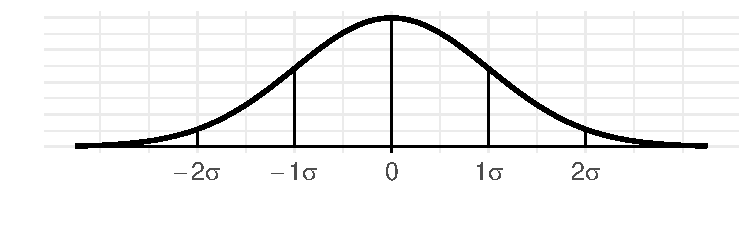
\includegraphics[width=\maxwidth]{img/mc-distribution-02-a-1} 

}







\begin{enumerate}
\item [\textbf{A} \msquare] Die Fläche rechts von $2\sigma$ ist der p-Wert mit $Pr(D|H_0)$ in der obigen Abbildung.
\item [\textbf{B} \msquare] Dargestellt ist eine Standardnormalverteilung.
\item [\textbf{C} \msquare] Die Fläche links von $-2\sigma$ ist der p-Wert mit $Pr(D|H_0)$ in der obigen Abbildung.
\item [\textbf{D} \msquare] Die Fläche unter der Kurve ist 1, wenn die Nullhypothese falsch ist. Wenn die Nullhypothese gilt, dann ist die Fläche $1-\alpha$. Somit ergibt sich auch eine Standardabweichung $\sigma$ mit $\alpha$ gleich 0.05 in beiden Fällen.
\item [\textbf{E} \msquare] Es liegen 68\% der Beobachtungen zwischen $\bar{y}\pm 1 \sigma$. Angezeigt durch die Fläche zwischen $-1\sigma$ und $1\sigma$ in der obigen Abbildung.
\end{enumerate} 

\section{Aufgabe \hfill (2 Punkte)}

%% --------------------------------------------------------------------
\ifcollection
\begin{flushright}
\tiny\vspace{-2Ex}
\textbf{\examinhaltstart}
\exammodulestatversuch $\;\bullet$
\exammodulebiostat
\vspace{-1Ex}
\end{flushright}
\fi
%% --------------------------------------------------------------------




Die empfohlene Mindestanzahl an Beobachtungen für die Visualisierung mit einem Boxplot sind...



\begin{enumerate}
\item [\textbf{A} \msquare] Wir brauchen fünf oder mehr Beobachtungen.
\item [\textbf{B} \msquare] Mindestens 20 Beobachtungen.
\item [\textbf{C} \msquare] 1 Beobachtung.
\item [\textbf{D} \msquare] Wir sollten eine Beobachtung mindestens pro Gruppe vorliegen haben.
\item [\textbf{E} \msquare] Die untere Grenze liegt bei einer Beobachtung.
\end{enumerate}

\section{Aufgabe \hfill (2 Punkte)}

%% --------------------------------------------------------------------
\ifcollection
\begin{flushright}
\tiny\vspace{-2Ex}
\textbf{\examinhaltstart}
\exammodulestatversuch $\;\bullet$
\exammodulebiostat
\vspace{-1Ex}
\end{flushright}
\fi
%% --------------------------------------------------------------------




Sie wollen in Ihrer Abschlussarbeit über eine explorative Datenanalyse überprüfen, ob Ihr gemessener Endpunkt einer Normalverteilung folgt. Welche drei Abbildungen eignen sich insbesondere für die Überprüfung?





\begin{enumerate}
\item [\textbf{A} \msquare] Violinplot, Scatterplot, Barplot
\item [\textbf{B} \msquare] Boxplot, Violinplot, Mosaicplot
\item [\textbf{C} \msquare] Barplot, Mosaicplot, Violinplot
\item [\textbf{D} \msquare] Histogramm, Densityplot, Dotplot
\item [\textbf{E} \msquare] Densityplot, Boxplot, Violinplot
\end{enumerate}

\section{Aufgabe \hfill (2 Punkte)}


%% --------------------------------------------------------------------
\ifcollection
\begin{flushright}
\tiny\vspace{-2Ex}
\textbf{\examinhaltstart}
\exammodulestatversuch $\;\bullet$
\exammodulebiostat
\vspace{-1Ex}
\end{flushright}
\fi
%% --------------------------------------------------------------------




Sie wollen eine ANOVA im Anschluss an Ihr Feldexperiment rechnen. Dafür muss Ihr gemessener Endpunkt die Annahme einer Varianzhomogenität genügen. Zur Überprüfung können Sie folgende Visualisierung nutzen. Welche entsprechende Regel zur Abschätzung der Annahme einer Varianzhomogenität kommt zur Anwendung?



\begin{enumerate}
\item [\textbf{A} \msquare] Nach dem Einlesen der Daten nutzen wir einen Barplot um zu schauen, ob alle Mittelwerte über alle Behandlungen in etwa gleich groß sind. Damit ist dann auch die Varianz in allen Behandlungen in etwa gleich.
\item [\textbf{B} \msquare] In einer explorativen Datanalyse nutzen wir den Boxplot. Dabei sollte der Median als dicke Linie in der Mitte der Box liegen. Dann können wir von einer Varianzhomogenität ausgehen.
\item [\textbf{C} \msquare] Einen Barplot. Die Mittelwerte müssen alle auf einer Höhe liegen. Die Fehlerbalken haben hier keine Informationen.
\item [\textbf{D} \msquare] In einer explorativen Datanalyse nutzen wir den Violinplot. Dabei sollte der Bauch am Rand liegen. Dann können wir von einer Varianzhomogenität ausgehen.
\item [\textbf{E} \msquare] Nach dem Einlesen der Daten nutzen wir einen Boxplot um zu schauen, ob alle Boxen über alle Behandlungen in etwa gleich groß sind. Damit ist dann auch das IQR in allen Behandlungen in etwa gleich.
\end{enumerate}
\section*{Statistische Testtheorie}  

\section{Aufgabe \hfill (2 Punkte)}

%% --------------------------------------------------------------------
\ifcollection
\begin{flushright}
\tiny\vspace{-2Ex}
\textbf{\examinhaltstart}
\exammodulemathstat $\;\bullet$
\exammodulestat $\;\bullet$
\exammodulestatbbv $\;\bullet$
\exammodulestatversuch $\;\bullet$
\exammodulebiostat
\vspace{-1Ex}
\end{flushright}
\fi
%% --------------------------------------------------------------------




Welche Aussage zum mathematische Ausdruck $Pr(D|H_0)$ ist richtig?



\begin{enumerate}
\item [\textbf{A} \msquare] Die Wahrscheinlichkeit für die Nullhypothese, wenn die Daten wahr sind.
\item [\textbf{B} \msquare] $Pr(D|H_0)$ stellt die Wahrscheinlichkeit die Teststatistik $T$ zu beobachten dar, wenn die Nullhypothese falsch ist.
\item [\textbf{C} \msquare] $Pr(D|H_0)$ ist die Wahrscheinlichkeit nicht die Daten $D$ zu beobachten sondern die Nullhypothese, wenn diese wahr ist.
\item [\textbf{D} \msquare] Die Inverse der Wahrscheinlichkeit unter der die Nullhypothese nicht mehr die Alternativehypothese überdeckt.
\item [\textbf{E} \msquare] $Pr(D|H_0)$ stellt die Wahrscheinlichkeit die Daten $D$ und somit die Teststatistik $T_D$ zu beobachten dar, wenn die Nullhypothese wahr ist.
\end{enumerate} 

\section{Aufgabe \hfill (2 Punkte)}

%% --------------------------------------------------------------------
\ifcollection
\begin{flushright}
\tiny\vspace{-2Ex}
\textbf{\examinhaltstart}
\exammodulemathstat $\;\bullet$
\exammodulestat $\;\bullet$
\exammodulestatbbv $\;\bullet$
\exammodulestatversuch $\;\bullet$
\exammodulebiostat
\vspace{-1Ex}
\end{flushright}
\fi
%% --------------------------------------------------------------------




Der Fehler 1. Art oder auch Signifikanzniveau $\alpha$ genannt, liegt bei
5\%. Welcher der folgenden Gründe für diese Festlegeung auf 5\% als Signifikanzschwelle ist richtig?



\begin{enumerate}
\item [\textbf{A} \msquare] In der Wissenschaft gibt es neben der Naturkonstante, die sich aus der Beobachtung der Welt ergibt, noch die Kulturkonstante, die von einer Gruppe Menschen selbstgewählt wird. Dabei ist $\alpha = 5\%$ eine Kulturkonstante und wurde somit eher zufällig gewählt.
\item [\textbf{B} \msquare] Als Kulturkonstante hat $\alpha = 5\%$ den Rang einer Naturkonstante und wurde nach langer Diskussion in der UN im Jahre 1983 festgesetzt. Damals auch schon mit der Zustimmung der UdSSR.
\item [\textbf{C} \msquare] Der Begründer der modernen Statistik, R. Fischer, hat die Grenze simuliert und berechnet. Dadurch ergibt sich dieser optimale Cut-Off.
\item [\textbf{D} \msquare] Auf einer Statistikkonferenz in Genf im Jahre 1942 wurde dieser Cut-Off nach langen Diskussionen festgelegt. Bis heute ist der Cut Off aber umstritten, da wegen dem 2. Weltkrieg viele Wissenschaftler nicht teilnehmen konnten.
\item [\textbf{E} \msquare] Der Wert ergab sich aus einer Auswertung von 1042 wissenschaftlichen Veröffentlichungen zwischen 1914 und 1948. Der Wert $5\%$ wurde in $28\%$ der Veröffentlichungen genutzt. Daher legte man sich auf diese Zahl fest.
\end{enumerate} 

\section{Aufgabe \hfill (2 Punkte)}

%% --------------------------------------------------------------------
\ifcollection
\begin{flushright}
\tiny\vspace{-2Ex}
\textbf{\examinhaltstart}
\exammodulemathstat $\;\bullet$
\exammodulestat $\;\bullet$
\exammodulestatbbv $\;\bullet$
\exammodulestatversuch $\;\bullet$
\exammodulebiostat
\vspace{-1Ex}
\end{flushright}
\fi
%% --------------------------------------------------------------------




Das statistische Testen basiert auf dem Falsifikationsprinzip. Es besagt,



\begin{enumerate}
\item [\textbf{A} \msquare] ... dass Modelle meist falsch sind und selten richtig.
\item [\textbf{B} \msquare] ... dass ein schlechtes Modell durch ein schlechteres Modell ersetzt wird. Die Wissenschaft lehnt ab und verifiziert nicht.
\item [\textbf{C} \msquare] ... dass in der Wissenschaft immer etwas falsch sein muss. Sonst gebe es keinen Fortschritt.
\item [\textbf{D} \msquare] ... dass Annahmen an statistische Modelle meist falsch sind.
\item [\textbf{E} \msquare] ... dass ein schlechtes Modell durch das Falsifikationsprinzip durch ein weniger schlechtes Modell ersetzt wird.
\end{enumerate}

\section{Aufgabe \hfill (2 Punkte)}

%% --------------------------------------------------------------------
\ifcollection
\begin{flushright}
\tiny\vspace{-2Ex}
\textbf{\examinhaltstart}
\exammodulemathstat $\;\bullet$
\exammodulestat $\;\bullet$
\exammodulestatbbv $\;\bullet$
\exammodulestatversuch $\;\bullet$
\exammodulebiostat
\vspace{-1Ex}
\end{flushright}
\fi
%% --------------------------------------------------------------------




Betrachten wir die Teststatistik aus einem abstrakteren Blickwinkel. Beim statistischen Testen wird das 	extit{signal} mit dem 	extit{noise} aus den Daten $D$ zu einer Teststatistik $T_D$ verrechnet. Welche der Formel berechnet korrekt die Teststatistik $T_D$?



\begin{enumerate}
\item [\textbf{A} \msquare] Es gilt $T_D = (signal \cdot noise)^2$. Der Effekt $signal$ wird mit der Varianz $noise$ gewichtet.
\item [\textbf{B} \msquare] Bei der Berechnung der Teststatistik $T_D$ gewichten wir den Effekt $signal$ mit der Varianz $noise$. Wir können verallgemeinert $T_D = \cfrac{signal}{noise^2}$ schreiben.
\item [\textbf{C} \msquare] Es gilt $T_D = \cfrac{noise}{signal}$. Der Effekt $noise$ wird mit der Varianz $signal$ gewichtet.
\item [\textbf{D} \msquare] Bei der Berechnung der Teststatistik $T_D$ gewichten wir den Effekt $signal$ mit der Varianz $noise$. Wir können verallgemeinert $T_D = \cfrac{signal}{noise}$ schreiben.
\item [\textbf{E} \msquare] Wir gewichten den Effekt $noise$ mit der Varianz $signal$ und erhalten $\cfrac{signal}{noise^2}$.
\end{enumerate}

%% ------------------------------------------------------------

\section{Aufgabe \hfill (2 Punkte)}

%% --------------------------------------------------------------------
\ifcollection
\begin{flushright}
\tiny\vspace{-2Ex}
\textbf{\examinhaltstart}
\exammodulemathstat $\;\bullet$
\exammodulestat $\;\bullet$
\exammodulestatbbv $\;\bullet$
\exammodulestatversuch $\;\bullet$
\exammodulebiostat
\vspace{-1Ex}
\end{flushright}
\fi
%% --------------------------------------------------------------------




Welche Aussage über den $p$-Wert und dem Signifikanzniveau $\alpha$ gleich 5\% ist richtig?



\begin{enumerate}
\item [\textbf{A} \msquare] Wir vergleichen mit dem $p$-Wert und dem Signifikanzniveau $\alpha$ absolute Werte auf einem Zahlenstrahl und damit den Unterschied der Teststatistiken, wenn die $H_0$ gilt.
\item [\textbf{B} \msquare] Wir vergleichen die Effekte des $p$-Wertes mit den Effekten der Signifikanzschwelle unter der Annahme der Nullhypothese. Dabei gilt, dass wir die Nullhypothese nur ablehnen können anhand des Falsifikationsprinzips.
\item [\textbf{C} \msquare] Wir vergleichen mit dem $p$-Wert und dem Signifikanzniveau $\alpha$ Wahrscheinlichkeiten und damit die absoluten Werte auf einem Zahlenstrahl, wenn die $H_0$ gilt.
\item [\textbf{D} \msquare] Wir schauen, ob der $p$-Wert größer ist als das Signifikanzniveau $\alpha$ und vergleichen somit Wahrscheinlichkeiten. Die Wahrscheinlichkeiten werden als Flächen unter der Kurve der Teststaistik dargestellt, wenn die $H_A$ gilt.
\item [\textbf{E} \msquare] Wir machen ein Aussage über die Flächen und der Kurve der Teststatistik, wenn die $H_0$ gilt. Dabei werden Wahrscheinlichkeiten vergleichen, die durch die Flächen unter der Kurve repräsentiert werden.
\end{enumerate}

\section{Aufgabe \hfill (2 Punkte)}

%% --------------------------------------------------------------------
\ifcollection
\begin{flushright}
\tiny\vspace{-2Ex}
\textbf{\examinhaltstart}
\exammodulemathstat $\;\bullet$
\exammodulestat $\;\bullet$
\exammodulestatbbv $\;\bullet$
\exammodulestatversuch $\;\bullet$
\exammodulebiostat
\vspace{-1Ex}
\end{flushright}
\fi
%% --------------------------------------------------------------------




Um die Testtheorie besser zu verstehen, mag es manchmal sinnvoll sein ein Beispiel aus dem Alltag zu wählen. Die Ergebnisse der Analyse durch einen statistischen Test können auch in grobe Analogie zur Wettervorhersage gebracht werden. Welche Aussage trifft am ehesten zu?



\begin{enumerate}
\item [\textbf{A} \msquare] In der Analogie der Durchschnittstemperatur: Wie oft tritt ein Effekt durchschnittlich ein? Wir erhalten eine Wahrscheinlichkeit für die Effekte. Zum Beispiel, wie hoch ist die Wahrscheinlichkeit für einen Mittelwert als Durchschnitt.
\item [\textbf{B} \msquare] In der Analogie der Wahrscheinlichkeit für Regen: ein statistischer Test erlaubt die Wahrscheinlichkeit für ein Ereignis abzuschätzen. Die Stärke des Effektes können wir nicht bestimmen.
\item [\textbf{C} \msquare] In der Analogie der Regenwahrscheinlichkeit in einem bestimmten Gebiet: ein statistischer Test gibt die Wahrscheinlichkeit für ein Ereignis in einem Experiment mit den Daten $D$ wieder und lässt sich kaum verallgemeinern.
\item [\textbf{D} \msquare] In der Analogie der Sonnenscheindauer: Wie lange kann mit einem entsprechenden Effekt gerechnet werden? Die Wahrscheinlichkeit für den Effekt gibt der statistische Test wieder.
\item [\textbf{E} \msquare] In der Analogie des Niederschlags oder Regenmenge: ein statistischer Test gibt die Stärke eines Effektes wieder. Zum Beispiel, wie hoch ist der Mittelwertsunterschied.
\end{enumerate}

\section{Aufgabe \hfill (2 Punkte)}

%% --------------------------------------------------------------------
\ifcollection
\begin{flushright}
\tiny\vspace{-2Ex}
\textbf{\examinhaltstart}
\exammodulemathstat $\;\bullet$
\exammodulestat $\;\bullet$
\exammodulestatbbv $\;\bullet$
\exammodulestatversuch $\;\bullet$
\exammodulebiostat
\vspace{-1Ex}
\end{flushright}
\fi
%% --------------------------------------------------------------------




Sie wollen eine Aussage über die untersuchte Population treffen. Dazu nutzen Sie einen statistischen Test. Können Sie eine valide Aussage aus einem statistischen Test erhalten?



\begin{enumerate}
\item [\textbf{A} \msquare] Ja, wir können die untersuchte Population nicht mit einem t-Test auswerten. Wir erhalten keine Aussage zur Population. Wir können aber den Effekt als Quelle der Relevanz nutzen.
\item [\textbf{B} \msquare] Ja, wir erhalten nur eine Aussage zu zwei Individuen. Ein statistischer Test liefert Informationen zu einem Individuum im Vergleich zu einem anderen Individuum.
\item [\textbf{C} \msquare] Ja, die untersuchte Population können wir mit einem statistischen Test auswerten. Wir erhalten dann eine Aussage zur Population.
\item [\textbf{D} \msquare] Nein, wir erhalten eine Aussage. Müssen aber das Individuum im Kontext der Population adjustieren.
\item [\textbf{E} \msquare] Nein, es ist nicht möglich die untersuchte Population mit einem t-Test auszuwerten. Wir erhalten dann leider keine Aussage zur Population.
\end{enumerate}

\section{Aufgabe \hfill (2 Punkte)}

%% --------------------------------------------------------------------
\ifcollection
\begin{flushright}
\tiny\vspace{-2Ex}
\textbf{\examinhaltstart}
\exammodulemathstat $\;\bullet$
\exammodulestat $\;\bullet$
\exammodulestatbbv $\;\bullet$
\exammodulestatversuch $\;\bullet$
\exammodulebiostat
\vspace{-1Ex}
\end{flushright}
\fi
%% --------------------------------------------------------------------




Sie rechnen einen statistischen Test und erhalten neben dem p-Wert noch einen Effekt wiedergegeben. Welche Aussage zum Effekt ist richtig?



\begin{enumerate}
\item [\textbf{A} \msquare] Der Effekt eines statistischen Tests beschreibt die mathematisch interpretierbare Ausgabe eines Tests. Damit ist der Effekt direkt mit dem Begriff der Signifikanz verbunden. Die Entscheidung über die Signifikanz trifft der Forschende unabhängig von der Relevanz eines statistsichen Tests.
\item [\textbf{B} \msquare] Der Forschende muss am Ende wissen, ob das Eregbnis eines Experiments relevant für seine Forschung ist. Dafür kann der Effekt eines statistischen Tests genutzt werden. Damit beschreibt der Effekt den biologischen interpretierbaren Teil einer Ausgabe eines Tests. Zum Beispiel der Unterschied zwischen zwei Anteilen.
\item [\textbf{C} \msquare] Der Effekt eines statistischen Tests beschreibt den Output oder die Wiedergabe eines Tests in einem Computer.
\item [\textbf{D} \msquare] Der Effekt eines statistischen Tests beschreibt die biologisch interpretierbare Ausgabe eines Tests. Damit ist der Effekt direkt mit dem Begriff der Signifikanz verbunden. Die Entscheidung über die Signifikanz trifft der Forschende unabhängig von der Relevanz eines statistsichen Tests.
\item [\textbf{E} \msquare] Der Effekt eines statistischen Tests beschreibt die biologisch interpretierbare Ausgabe eines Tests. Moderen Algorithmen liefern keine Effekte mehr sondern nur noch bedingte Wahrscheinlichkeiten. Der Effekt spielt in der modernen Statistik keine Rollen mehr.
\end{enumerate}

\section{Aufgabe \hfill (2 Punkte)}

%% --------------------------------------------------------------------
\ifcollection
\begin{flushright}
\tiny\vspace{-2Ex}
\textbf{\examinhaltstart}
\exammodulemathstat $\;\bullet$
\exammodulestat $\;\bullet$
\exammodulestatbbv $\;\bullet$
\exammodulestatversuch $\;\bullet$
\exammodulebiostat
\vspace{-1Ex}
\end{flushright}
\fi
%% --------------------------------------------------------------------



Sie führen einen agrarwissenschaftlichen Versuch durch. Dafür müssen Sie als ersten Schritt Ihre Versuchseinheiten zufällig den Behandlungen zuordnen. Dieses zufällige Zuordnen nennt man in der Statistik eine Randomisierung. Warum ist die Randomisierung so wichtig für das Gelingen eines Versuchs?



\begin{enumerate}
\item [\textbf{A} \msquare] Randomisierung bringt starke Unstrukturiertheit in das Experiment und erlaubt erst von der Stichprobe auf die Grundgesamtheit zurückzuschliessen.
\item [\textbf{B} \msquare] Randomisierung war bis 1952 bedeutend, wurde dann aber in Folge besserer Rechnerleistung nicht mehr verwendet. Aktuelle Statistik nutzt keine Randomisierung mehr.
\item [\textbf{C} \msquare] Randomisierung sorgt für Strukturgleichheit und erlaubt erst von der Stichprobe auf die Grundgesamtheit zurückzuschliessen.
\item [\textbf{D} \msquare] Strukturgleichheit ist durch Randomisierung gegeben. Leider hilft die Randomisierung noch nicht um von der Stichprobe auf die Grundgesamtheit zu schließen. Deshalb wurde das Falsifikationsprinzip entwickelt.
\item [\textbf{E} \msquare] Durch eine Randomisierung können wir nicht von Strukturgleichheit zwischen der Stichprobe und der Grundgesamtheit ausgehen.
\end{enumerate}

\section{Aufgabe \hfill (2 Punkte)}

%% --------------------------------------------------------------------
\ifcollection
\begin{flushright}
\tiny\vspace{-2Ex}
\textbf{\examinhaltstart}
\exammodulemathstat $\;\bullet$
\exammodulestat $\;\bullet$
\exammodulestatbbv $\;\bullet$
\exammodulestatversuch $\;\bullet$
\exammodulebiostat
\vspace{-1Ex}
\end{flushright}
\fi
%% --------------------------------------------------------------------




Wenn Sie im Allgemeinen einen statistischen Test rechnen, dann kommen Sie um eine statistische Hypothese $H$ nicht herum. Welche Aussage über statistische Hypothesen ist richtig?



\begin{enumerate}
\item [\textbf{A} \msquare] Mit der Nullhypothese $H_A$ und der Alternativehypothese $H_0$ gibt es zwei Hypothesen, die aber selten genutzt werden.
\item [\textbf{B} \msquare] Es gibt ein statistisches Hypothesenpaar mit der Hypothese für und gegen die wissenschaftliche Fragestellung. Die Hypothesen werden $H_{pro}$ und $H_{contra}$ bezeichnet.
\item [\textbf{C} \msquare] Ein statistisches Hypothesenpaare gibt es. Zum einen die Nullhypothese und zum anderen die Alternativehypothese. Es ist aber nur notwendig die Alternative anzugeben, da die Nullhypothese nicht beim Testen benötigt wird.
\item [\textbf{D} \msquare] Ein statistisches Hypothesenpaare gibt es. Zum einen die Nullhypothese $H_0$ und zum anderen die Alternativehypothese $H_A$ oder $H_1$
\item [\textbf{E} \msquare] Die Hypothesen $H_0$ und $H_A$ sind rein prosarischer Natur und bilden keinen mathematischen Hintergrund ab. In der Statistik wird die wissenschaftliche Fragestellung getestet. Daher stehen auch die verständlichen Hypothesen im Mittelpunkt der biologischen Interpretation.
\end{enumerate}

\section{Aufgabe \hfill (2 Punkte)}

%% --------------------------------------------------------------------
\ifcollection
\begin{flushright}
\tiny\vspace{-2Ex}
\textbf{\examinhaltstart}
\exammodulemathstat $\;\bullet$
\exammodulestat $\;\bullet$
\exammodulestatbbv $\;\bullet$
\exammodulestatversuch $\;\bullet$
\exammodulebiostat
\vspace{-1Ex}
\end{flushright}
\fi
%% --------------------------------------------------------------------




In der Theorie zur statistischen Testentscheidung kann folgende Aussage
in welche richtige Analogie gesetzt werden?

\begin{center}
\textit{$H_0$ beibehalten obwohl die $H_0$ falsch ist}
\end{center}



\begin{enumerate}
\item [\textbf{A} \msquare] Dem $\beta$-Fehler mit der Analogie eines brennenden Hauses: \textit{Fire without alarm}.
\item [\textbf{B} \msquare] \textit{Alarm without fire}, dem $\alpha$-Fehler in der Analogie eines Rauchmelders.
\item [\textbf{C} \msquare] \textit{Fire without alarm}, dem $\beta$-Fehler als Analogie von Rauch im Haus.
\item [\textbf{D} \msquare] In die Analogie eines Rauchmelders: \textit{Fire without alarm}, dem $\beta$-Fehler.
\item [\textbf{E} \msquare] In die Analogie eines Rauchmelders: \textit{Alarm without fire police}, dem $\alpha$-Fehler.
\end{enumerate}

\section{Aufgabe \hfill (2 Punkte)}

%% --------------------------------------------------------------------
\ifcollection
\begin{flushright}
\tiny\vspace{-2Ex}
\textbf{\examinhaltstart}
\exammodulestat $\;\bullet$
\exammodulestatbbv $\;\bullet$
\exammodulestatversuch $\;\bullet$
\exammodulebiostat
\vspace{-1Ex}
\end{flushright}
\fi
%% --------------------------------------------------------------------




Sie sollen in Ihrer Abschlussarbeit die Relevanz und die Signifikanz in einer statistischen Maßzahl vereinen. Welche Aussage ist richtig?



\begin{enumerate}
\item [\textbf{A} \msquare] Einem Konfidenzintervall. Das Konfidenzinterval bringt durch eine Visualisierung und zwei Intervallgrenzen die Möglichkeit mit, eine Relevanzschwelle neben der definierten Signifikanzschwelle zu definieren.
\item [\textbf{B} \msquare] Der p-Wert. Durch den Vergleich mit $\alpha$ lässt sich über die Signifikanz entscheiden und der $\beta$-Fehler erlaubt über die Power eine Einschätzung der Relevanz.
\item [\textbf{C} \msquare] Das OR. Als Chancenverhältnis gibt es das Verhältnis von Relevanz und Signifikanz wieder.
\item [\textbf{D} \msquare] Die Teststatistik. Durch den Vergleich von $T_c$ zu $T_k$ ist es m{"o}glich die $H_0$ abzulehnen. Die Relevanz ergibt sich aus der Fläche rechts vom dem $T_c$-Wert.
\item [\textbf{E} \msquare] Das $\Delta$. Durch die Effektstärke haben wir einen Wert für die Relevanz, die vom Anwender bewertet werden muss. Da $\Delta$ antiproportional zum p-Wert ist, bedeutet auch ein hohes $\Delta$ ein sehr kleinen p-Wert.
\end{enumerate}

\section{Aufgabe \hfill (2 Punkte)}

%% --------------------------------------------------------------------
\ifcollection
\begin{flushright}
\tiny\vspace{-2Ex}
\textbf{\examinhaltstart}
\exammodulestatversuch $\;\bullet$
\exammodulebiostat
\vspace{-1Ex}
\end{flushright}
\fi
%% --------------------------------------------------------------------




In der Bio Data Science wird häufig mit sehr großen Datensätzen gerechnet. Historisch ergibt sich nun ein Problem bei der Auswertung der Daten und deren Bewertung hinsichtlich der Signifikanz. Welche Aussage ist richtig?





\begin{enumerate}
\item [\textbf{A} \msquare] Mehr Fallzahl in Datensätzen bedeutet mehr signifikante Ergebnisse, da in mehr Daten auch mehr Informationen beinhaltet sind. Deshalb lohnen sich riesige Datensätze, die durch die vielen signifikanten Ergebnisse auch eine Menge an relevanten Erkenntnissen liefern.
\item [\textbf{B} \msquare] Aktuell werden zu grosse Datensätze für die gänigige Statistik gemessen. Daher wendet man maschinelle Lernverfahren für kausale Modelle an. Hier ist die Relevanz gleich Signifikanz.
\item [\textbf{C} \msquare] Eine erhöhte Fallzahl führt automatisch zu mehr signifikanten Ergebnissen auch wenn der Effekt klein ist und damit nicht relevant. Dadurch sind die Informationen zur Signifikanz in riesigen Datensätzen schwer zu verwerten, da fast alle Vergleiche signifikant sind.
\item [\textbf{D} \msquare] Riesige Datensätz haben mehr Fallzahl was zur $\alpha$-Inflation führt. Durch eine Adjustoerung kann dem Problem entgegengewirkt werden.
\item [\textbf{E} \msquare] Big Data ist ein Problem der parametrischen Statistik. Parameter lassen sich nur auf kleinen Datensätzen berechnen, da es sich sonst nicht mehr um eine Stichprobe im engen Sinne der Statistik handelt.
\end{enumerate}

\section{Aufgabe \hfill (2 Punkte)}

%% --------------------------------------------------------------------
\ifcollection
\begin{flushright}
\tiny\vspace{-2Ex}
\textbf{\examinhaltstart}
\exammodulestatversuch $\;\bullet$
\exammodulebiostat
\vspace{-1Ex}
\end{flushright}
\fi
%% --------------------------------------------------------------------




Im Rahmen Ihrer Abschlussarbeit werten Sie ein Experiment mit Ferkel aus. Es geht um die Leistungssteigerung der Ferkelproduktion. Sie messen jeweils die Gewichtszunahme der Ferkel. Die Ferkel einer Muttersau sind dabei...



\begin{enumerate}
\item [\textbf{A} \msquare] Abhängig von der Stallanlage und des Experiments können die Ferkel abhängig oder unabhängig sein. Allgmein gilt, dass Ferkel von unterschiedlichen Sauen näher miteinander verwandt sind als Ferkel von gleichen Sauen. Das Fisher-Axiom.
\item [\textbf{B} \msquare] Untereinander unabhängig. Die Ferkel sind eigenständig und benötigen keine zusätzliche Behandlung.
\item [\textbf{C} \msquare] Untereinander stark korreliert. Die Ferkel sind von einer Mutter und sommit miteinander korreliert. Dies wird in der Statistik jedoch meist nicht modelliert.
\item [\textbf{D} \msquare] Untereinander abhängig, wenn die Mütter ebenfalls miteinander verwandt sind. Erst die Abhängigkeit 2. Grades wird in der Statistik modelliert.
\item [\textbf{E} \msquare] Die Ferkel stammen vom gleichen Muttertier und haben vermutlich eine ähnlichere Varianzstruktur als die Ferkel von anderen Sauen. Die Ferkel sind untereinander über die Mutter abhängig.
\end{enumerate}

\section{Aufgabe \hfill (2 Punkte)}

%% --------------------------------------------------------------------
\ifcollection
\begin{flushright}
\tiny\vspace{-2Ex}
\textbf{\examinhaltstart}
\exammodulestatversuch $\;\bullet$
\exammodulebiostat
\vspace{-1Ex}
\end{flushright}
\fi
%% --------------------------------------------------------------------






Sie rechnen einen statistischen Test und wollen anhand des 95\%-Konfidenzintervalls eine Entscheidung gegen die Nullhypothese treffen. Welche Aussage ist richtig?





\begin{enumerate}
\item [\textbf{A} \msquare] Wir betrachten das Ganze Intervall des 95\%-Konfidenzintervalls. Liegt die Null mit in dem Intervall, dann kann die Nullhypothese abgelehnt werden.
\item [\textbf{B} \msquare] Ist $Pr(D|H_0)$ kleiner als das Signifikanzniveau $\alpha$ gleich $5\%$ dann wird die Nullhypothese $H_0$ abgelehnt.
\item [\textbf{C} \msquare] Liegt das berechnete Intervall über dem kritische Wert $T_{\alpha = 5\%}$, dann kann die Nullhypothese nicht abgelehnt werden.
\item [\textbf{D} \msquare] Anhand des 95\%-Konfidenzintervalls lässt sich wie folgt eine Entscheidung treffen. Liegt der Wert über oder gleich dem Signifikanzniveau $\alpha$ dann kann die Nullhypothese abgelehnt werden.
\item [\textbf{E} \msquare] Der kritische Wert $T_{\alpha = 5\%}$ ist tabelarisch festgelegt und gegeben. Ist $T_{D}$ größer als der kritische Wert, kann die Nullhypothese abgelehnt werden
\end{enumerate}

\section{Aufgabe \hfill (2 Punkte)}

%% --------------------------------------------------------------------
\ifcollection
\begin{flushright}
\tiny\vspace{-2Ex}
\textbf{\examinhaltstart}
\exammodulebiostat
\vspace{-1Ex}
\end{flushright}
\fi
%% --------------------------------------------------------------------




Welche Aussage über die \textit{Power} ist richtig?



\begin{enumerate}
\item [\textbf{A} \msquare] Die Power $1-\beta$ wird auf 80\% gesetzt. Alle statistischen Tests sind so konstruiert, dass die $H_A$ mit 80\% \textit{bewiesen wird}.
\item [\textbf{B} \msquare] Alle statistischen Tests sind so konstruiert, dass die $H_A$ mit 20\% \textit{bewiesen wird}. Die Power ist $1-\beta$ mit $\beta$ gleich 80\% gesetzt.
\item [\textbf{C} \msquare] Die Power beschreibt die Wahrscheinlichkeit die $H_A$ abzulehnen. Wir testen die Power jedoch nicht.
\item [\textbf{D} \msquare] Die Power ist nicht in der aktuellen Testthorie mehr vertreten. Wir rechnen nur noch mit dem Fehler 1. Art.
\item [\textbf{E} \msquare] Es gilt $\alpha + \beta = 1$ und somit liegt $\beta$ meist bei 95\%.
\end{enumerate}
\section*{Statistische Tests für Gruppenvergleiche} 

\section{Aufgabe \hfill (2 Punkte)}

%% --------------------------------------------------------------------
\ifcollection
\begin{flushright}
\tiny\vspace{-2Ex}
\textbf{\examinhaltstart}
\exammodulemathstat $\;\bullet$
\exammodulestat $\;\bullet$
\exammodulestatbbv 
\vspace{-1Ex}
\end{flushright}
\fi
%% --------------------------------------------------------------------




Welche Aussage über den t-Test im Allgmeinen ist richtig? Berücksichtigen Sie den Welch t-Test wie auch den Student t-Test!



\begin{enumerate}
\item [\textbf{A} \msquare] Der t-Test vergleicht die Mittelwerte von zwei Gruppen unter der strikten Annahme von Varianzhomogenität. Sollte keine Varianzhomogenität vorliegen, so gibt es keine Möglichkeit den t-Test in einer Variante anzuwenden.
\item [\textbf{B} \msquare] Der t-Test testet generell zu einem erhöhten $\alpha$-Niveau von 20\%.
\item [\textbf{C} \msquare] Der t-Test ist ein Vortest der ANOVA und basiert daher auf dem Vergleich von Streuungsparametern
\item [\textbf{D} \msquare] Der t-Test vergleicht die Varianzen von mindestens zwei oder mehr Gruppen
\item [\textbf{E} \msquare] Der t-Test vergleicht zwei Gruppen indem die Mittelwerte miteinander verglichen werden.
\end{enumerate}

\section{Aufgabe \hfill (2 Punkte)}

%% --------------------------------------------------------------------
\ifcollection
\begin{flushright}
\tiny\vspace{-2Ex}
\textbf{\examinhaltstart}
\exammodulemathstat $\;\bullet$
\exammodulestat $\;\bullet$
\exammodulestat $\;\bullet$
\exammodulestatbbv $\;\bullet$
\exammodulestatversuch $\;\bullet$
\exammodulebiostat
\vspace{-1Ex}
\end{flushright}
\fi
%% --------------------------------------------------------------------




Die folgende Abbildung enthält die Daten aus einer Studie zur Bewertung der Wirkung des Mikronährstoff Nitrat auf den Ertrag in t/ha von Weizen im Vergleich zu einer Kontrolle. Der Versuch wurde in 6 Parzellen pro Gruppe durchgeführt. Welche Aussage im Bezug auf eine statistische Auswertung ist richtig?



{\centering 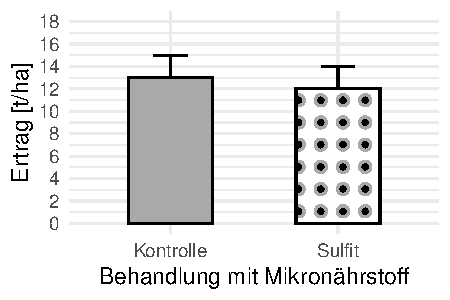
\includegraphics[width=\maxwidth]{img/mc-testing-ttest-02-1} 

}







\begin{enumerate}
\item [\textbf{A} \msquare] Der Test deutet auf einen signifikanten Unterschied hin. Der Effekt liegt vermutlich bei 1.
\item [\textbf{B} \msquare] Es liegt ein signifikanter Unterschied vor. Der Effekt liegt bei 0.1.
\item [\textbf{C} \msquare] Nach Betrachtung des Barplots liegt kein signifikanter Unterschied vor. Der Effekt kann nicht bei einem t-Test aus Barplots bestimmt werden.
\item [\textbf{D} \msquare] Die Barplots deuten auf kein signifikanten Unterschied. Der Effekt liegt vermutlich bei 1.
\item [\textbf{E} \msquare] Die Barplots deuten auf keinen signifikanten Unterschied. Der Effekt liegt vermutlich bei 1. Wir müssen aber einen Posthoc-Test rechnen um den Effekt wirklich bestimmen zu können.
\end{enumerate}

\section{Aufgabe \hfill (2 Punkte)}

%% --------------------------------------------------------------------
\ifcollection
\begin{flushright}
\tiny\vspace{-2Ex}
\textbf{\examinhaltstart}
\exammodulestatversuch $\;\bullet$
\exammodulebiostat
\vspace{-1Ex}
\end{flushright}
\fi
%% --------------------------------------------------------------------





In Ihrer Abschlussarbeit betrachten Sie die Effekte von einer Behandlung vor und nach der Gabe eines Vitamins. Sie müssen einen gepaarten t-Test rechnen. Welche Aussage ist richtig?



\begin{enumerate}
\item [\textbf{A} \msquare] Der gepaarte t-Test nutzt die Varianz der Beobachtungen jeweils paarweise und bildet dafür eine verbundene Stichprobe. Dieser Datensatz $d$ dient dann zur Differenzbildung.
\item [\textbf{B} \msquare] Der gepaarte t-Test wird gerechnet, wenn die Beobachtungen nicht unabhängig voneinander sind. Wir messen wiederholt an dem gleichen Probanden oder Tier oder Pflanze. Wir bilden die Differenzen um den gepaarten t-Test rechnen zu können.
\item [\textbf{C} \msquare] Abhängige Beobachtungen müssen gesondert in einem gepaarten t-Test modelliert werden. Wenn wiederholt an dem gleichen Tier oder Pflanze gemessen wird, dann bilden wir den Quotienten zwischen den beiden Zeitpunkten. Auf den Quotienten rechnen wir den gepaarten t-Test.
\item [\textbf{D} \msquare] Der gepaarte t-Test wird genutzt, wenn die Differenzen der Beobachtungen verbunden sind und wir dadurch die Unabhäängigkeit nicht mehr vorliegen haben.
\item [\textbf{E} \msquare] Wenn die Beobachtungen unabhängig voneinander sind, rechnen wir einen gepaarten t-Test. Messen wir wiederholt an dem gleichen Tier oder Pflanze dann bilden wir das Produkt zwischen den zwei Messpunkten.
\end{enumerate}

\section{Aufgabe \hfill (2 Punkte)}

%% --------------------------------------------------------------------
\ifcollection
\begin{flushright}
\tiny\vspace{-2Ex}
\textbf{\examinhaltstart}
\exammodulestatversuch $\;\bullet$
\exammodulebiostat
\vspace{-1Ex}
\end{flushright}
\fi
%% --------------------------------------------------------------------




Sie führen paarweise t-Tests für alle Vergleiche der verschiedenen Rapssorten in Ihrem Experiment durch. Nach der Adjustierung für multiples Testen ist kein p-Wert unter der $\alpha$-Schwelle. Ihr Experiment beinhaltet drei Rapssorten und eine ANOVA ergibt $p = 0.049$ für den Ertrag. Sie schauen sich auch die rohen, unadjustierten p-Werte an und finden hier als niedrigsten p-Wert $p_{3-2} = 0.051$. Welche Aussage ist richtig?




\begin{enumerate}
\item [\textbf{A} \msquare] Das ist kein Wunder. Die ANOVA testet nicht auf der gesamten Fallzahl und die paarweisen t-Tests gewinnen immer eine oder mehr Gruppen als Fallzahl dazu. Mit steigender Fallzahl sind mehr signifikante Unterschiede zu erwarten. Die p-Werte unterscheiden sich numerisch auch kaum.
\item [\textbf{B} \msquare] Hier kommt der Effekt der stiegenden Fallzahl auf die Anzahl an signifikante Ergebnisse zu tragen. Da die ANOVA auf mehr Fallzahl testet als die einzelnen paarweisen t-Tests, kann die ANOVA leichter einen signifikanten Unterscheid nachweisen. Die p-Werte sind immer etwas kleiner als bei den t-Tests.
\item [\textbf{C} \msquare] Die ANOVA testet auf der gesamten Fallzahl. Es wäre besser die ANOVA auf der gleichen Fallzahl wie die einzelnen t-Tests zu rechnen.
\item [\textbf{D} \msquare] Die adjustierten p-Werte deuten in die richtige Richtung. Zusammen mit den nicht signifikanten rohen p-Werten ist von einem Fehler in der ANOVA auszugehen.
\item [\textbf{E} \msquare] Das Beispiel kann so nicht auftreten, da die ANOVA und die t-Tests algorithmisch miteinander verschränkt sind.
\end{enumerate}
\section*{ANOVA}

\section{Aufgabe \hfill (2 Punkte)}

%% --------------------------------------------------------------------
\ifcollection
\begin{flushright}
\tiny\vspace{-2Ex}
\textbf{\examinhaltstart}
\exammodulemathstat $\;\bullet$
\exammodulestat $\;\bullet$
\exammodulestatbbv $\;\bullet$
\exammodulestatversuch $\;\bullet$
\exammodulebiostat
\vspace{-1Ex}
\end{flushright}
\fi
%% --------------------------------------------------------------------






Sie führen einen Versuch mit einer Behandlung und drei Faktorleveln durch. Danach rechnen Sie eine einfaktorielle ANOVA und es ergibt sich ein $\eta^2 = 0.31$. Welche Aussage ist richtig?



\begin{enumerate}
\item [\textbf{A} \msquare] Das $\eta^2$ beschreibt den Anteil der Varianz, der von den Behandlungsbedingungen nicht erkl{"a}rt wird. Somit der Rest an nicht erkl{"a}rbarer Varianz.
\item [\textbf{B} \msquare] Die Berechnung von $\eta^2$ ist ein Wert f{"u}r die Interaktion.
\item [\textbf{C} \msquare] Das $\eta^2$ ist ein Wert f{"u}r die G{"u}te der ANOVA. Je kleiner desto besser. Ein $\eta^2$ von 0 bedeutet ein perfektes Modell mit keiner Abweichung. Die Varianz ist null.
\item [\textbf{D} \msquare] Das $\eta^2$ ist die Korrelation der ANOVA. Mit der Ausnahme, dass 0 der beste Wert ist.
\item [\textbf{E} \msquare] Das $\eta^2$ ist damit mit dem $R^2$ aus der linearen Regression zu vergleichen und beschreibt den Anteil der Varianz, der von den Behandlungsbedingungen erkl{"a}rt wird.
\end{enumerate}

\section{Aufgabe \hfill (2 Punkte)}

%% --------------------------------------------------------------------
\ifcollection
\begin{flushright}
\tiny\vspace{-2Ex}
\textbf{\examinhaltstart}
\exammodulemathstat $\;\bullet$
\exammodulestat $\;\bullet$
\exammodulestatbbv $\;\bullet$
\exammodulestatversuch $\;\bullet$
\exammodulebiostat
\vspace{-1Ex}
\end{flushright}
\fi
%% --------------------------------------------------------------------










\begin{enumerate}
\item [\textbf{A} \msquare] Das $\eta^2$ beschreibt den Anteil der Varianz, der durch den Forschenden entsteht. Es gilt die Regel, dass ca. 70\% der Varianz eines Versuches durch die Versuchsdurchführung entstehen sollen.
\item [\textbf{B} \msquare] Es werden 28\% der Varianz durch den Versuch erklärt. Das $\eta^2$ beschreibt den Anteil der Varianz, der durch Fehler in der Versuchsdurchführung entsteht.
\item [\textbf{C} \msquare] Es werden 72\% der Varianz durch die Behandlung erklärt. Das $\eta^2$ beschreibt den Anteil der Varianz, der von den unterschiedlichen Behandlungsbedingungen nicht erklärt wird.
\item [\textbf{D} \msquare] Das $\eta^2$ beschreibt den Anteil der Varianz, der von den Umweltbedingungen erklärt wird. Daher werden 28\% der Varianz durch die Umweltbedingungen erklärt. Der Anteil der Varianz durch die Behandlungsgruppen ist dann 72\%.
\item [\textbf{E} \msquare] Das $\eta^2$ beschreibt den Anteil der Varianz, der von den Behandlungsbedingungen erklärt wird. Daher werden 28\% der Varianz erklärt.
\end{enumerate}

\section{Aufgabe \hfill (2 Punkte)}

%% --------------------------------------------------------------------
\ifcollection
\begin{flushright}
\tiny\vspace{-2Ex}
\textbf{\examinhaltstart}
\exammodulemathstat $\;\bullet$
\exammodulestat $\;\bullet$
\exammodulestatbbv $\;\bullet$
\exammodulestatversuch $\;\bullet$
\exammodulebiostat
\vspace{-1Ex}
\end{flushright}
\fi
%% --------------------------------------------------------------------




Sie rechnen eine einfaktorielle ANOVA und erhalten eine Teststatistik. Nun müssen Sie diese Teststatistik interpretieren. Welche Aussage ist richtig?



\begin{enumerate}
\item [\textbf{A} \msquare] Die ANOVA berechnet die T-Statistik indem den Mittelwertsunterschied der Gruppen simultan durch die Standardabweichung der Gruppen teilt. Wenn die T-Statistik h{"o}her als 1.96 ist, kann die Nullhypothese abgelehnt werden.
\item [\textbf{B} \msquare] Die ANOVA berechnt die F-Statistik aus den SS Behandlung geteilt durch die SS Fehler.
\item [\textbf{C} \msquare] Wenn die F-Statistik kleiner als der kritische Wert ist kann die Nullhypothese nicht abgelehnt werden. Die F-Statistik ist der Quotient der MS der Behandlung durch die MS des Fehlers.
\item [\textbf{D} \msquare] Wenn die F-Statistik höher ist als der kritische Wert kann die Nullhypothese nicht abgelehnt werden. Die F-Statistik ist die Differenz der MS der Behandlung durch die MS des Fehlers.
\item [\textbf{E} \msquare] Die ANOVA berechnet die F-Statistik indem die MS des Fehlers durch die MS der Behandlung geteilt werden. Wenn die F-Statistik sich der 1 ann{"a}hert kann die Nullhypothese nicht abgelehnt werden.
\end{enumerate}

\section{Aufgabe \hfill (2 Punkte)}

%% --------------------------------------------------------------------
\ifcollection
\begin{flushright}
\tiny\vspace{-2Ex}
\textbf{\examinhaltstart}
\exammodulemathstat $\;\bullet$
\exammodulestat $\;\bullet$
\exammodulestatbbv $\;\bullet$
\exammodulestatversuch $\;\bullet$
\exammodulebiostat
\vspace{-1Ex}
\end{flushright}
\fi
%% --------------------------------------------------------------------




Die ANOVA ist ein statistisches Verfahren welches häufig in den Auswertungen von Experimenten in den Agrarwissenschaften angewendet
wird. Dabei wird die ANOVA als ein erstes statistischen Werkzeug für die
Übersicht über die Daten benutzt. Eine ANOVA testet dabei...



\begin{enumerate}
\item [\textbf{A} \msquare] ... den Unterschied zwischen der Varianz in den verschiedenen Behandlungsguppen und der Varianz in einer der Behandlungsgruppen. Wenn die ANOVA signifikant ist, muss über einen Posthoc-Test nachgedacht werden um den signifikanten Unterschied in einer der Gruppen exakt zu bestimmen.
\item [\textbf{B} \msquare] ... den Unterschied zwischen der Varianz über alle Behandlungsgruppen und der Varianz aus verschiedenen Behandlungsguppen. Wenn die ANOVA signifikant ist, muss ein Posthoc-Test angeschlossen werden.
\item [\textbf{C} \msquare] ... den Unterschied zwischen der F-Statistik anhand der Varianz der Gruppen. Wenn die F-Statistik exakt 0 ist, kann die Nullhypothese abgelehnt werden.
\item [\textbf{D} \msquare] ... den Unterschied zwischen der Varianz ausgelöst durch alle Behandlungsgruppen und der Varianz aus globalen Behandlungsguppen der Kontrollen. Wenn die ANOVA nicht signifikant ist, muss ein Posthoc-Test ausgeschlossen werden.
\item [\textbf{E} \msquare] ... den Unterschied zwischen der Mittelwerte und der Varianz aus verschiedenen Behandlungsguppen. Wenn die ANOVA signifikant ist, ist bekannt welcher Vergleich konkret unterschiedlich ist.
\end{enumerate}

\section{Aufgabe \hfill (2 Punkte)}

%% --------------------------------------------------------------------
\ifcollection
\begin{flushright}
\tiny\vspace{-2Ex}
\textbf{\examinhaltstart}
\exammodulestatversuch $\;\bullet$
\exammodulebiostat
\vspace{-1Ex}
\end{flushright}
\fi
%% --------------------------------------------------------------------




Die folgende Abbildung enthält die Daten aus einer Studie zur Bewertung der Wirkung von Vitamin E auf das Zahnwachstum bei Schweine. Der Versuch wurde an 56 Tieren durchgeführt, wobei jedes Tier eine von  drei Vitamin-C-Dosen (0.5, 1 und 1.5 mg/Tag) über eine von zwei Verabreichungsmethoden erhielt. Welche Aussage ist richtig im Bezug auf eine zweifaktorielle ANOVA?



{\centering 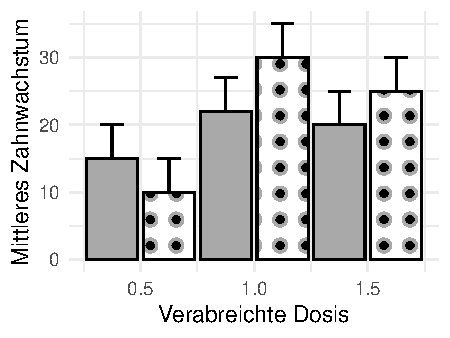
\includegraphics[width=\maxwidth]{img/mc-anova-02-a-1} 

}







\begin{enumerate}
\item [\textbf{A} \msquare] Eine Korrelation liegt vor $(p \leq 0.05)$.
\item [\textbf{B} \msquare] Keine Interaktion liegt vor $(p \leq 0.05)$.
\item [\textbf{C} \msquare] Das Bestimmtheitsmaß $R^2$ ist klein.
\item [\textbf{D} \msquare] Eine positive Interaktion liegt vor $(\rho \leq -0.5)$ 
\item [\textbf{E} \msquare] Eine mittlere bis starke Interaktion liegt vor $(p \leq 0.05)$
\end{enumerate}
\section*{Multiple Gruppenvergleiche} 

\section{Aufgabe \hfill (2 Punkte)}

%% --------------------------------------------------------------------
\ifcollection
\begin{flushright}
\tiny\vspace{-2Ex}
\textbf{\examinhaltstart}
\exammodulestatversuch $\;\bullet$
\exammodulebiostat
\vspace{-1Ex}
\end{flushright}
\fi
%% --------------------------------------------------------------------




Sie haben folgende unadjustierten p-Werte gegeben: 0.21, 0.34, 0.42 und 0.89. Sie adjustieren die p-Werte nach
Bonferroni. Welche Aussage ist richtig?



\begin{enumerate}
\item [\textbf{A} \msquare] Nach der Bonferroni-Adjustierung ergeben sich die adjustierten p-Werte von 0.84, 1.36, 1.68 und 3.56. Die adjustierten p-Werte werden zu einem $\alpha$-Niveau von 5\% verglichen.
\item [\textbf{B} \msquare] Nach der Bonferroni-Adjustierung ergeben sich die adjustierten p-Werte von 0.0525, 0.085, 0.105 und 0.2225. Die adjustierten p-Werte werden zu einem $\alpha$-Niveau von 1.25\% verglichen.
\item [\textbf{C} \msquare] Nach der Bonferroni-Adjustierung ergeben sich die adjustierten p-Werte von 0.84, 1, 1 und 1. Die adjustierten p-Werte werden zu einem $\alpha$-Niveau von 1.25\% verglichen.
\item [\textbf{D} \msquare] Nach der Bonferroni-Adjustierung ergeben sich die adjustierten p-Werte von 0.0525, 0.085, 0.105 und 0.2225. Die adjustierten p-Werte werden zu einem $\alpha$-Niveau von 5\% verglichen.
\item [\textbf{E} \msquare] Nach der Bonferroni-Adjustierung ergeben sich die adjustierten p-Werte von 0.84, 1, 1 und 1. Die adjustierten p-Werte werden zu einem $\alpha$-Niveau von 5\% verglichen.
\end{enumerate}

\section{Aufgabe \hfill (2 Punkte)}

%% --------------------------------------------------------------------
\ifcollection
\begin{flushright}
\tiny\vspace{-2Ex}
\textbf{\examinhaltstart}
\exammodulestatversuch $\;\bullet$
\exammodulebiostat
\vspace{-1Ex}
\end{flushright}
\fi
%% --------------------------------------------------------------------




Auf wissenschaftlichen Postern finden Sie unter Abbildungen häufig die Abbkürzung \textit{CLD}. Für welchen statistischen Fachbegriff steht die Abbkürzung und wie interpretieren Sie ein \textit{CLD}?



\begin{enumerate}
\item [\textbf{A} \msquare] Compound letter display. Gleichheit in dem Outcomes wird durch den gleichen Buchstaben oder Symbol dargestellt. Teilweise ist die Interpretation des Verbunds (eng. compound) herausfordernd, da wir ja nach dem Unterschied suchen.
\item [\textbf{B} \msquare] Compact letter detection. Gleichheit in den Behandlungen wird durch den gleichen Buchstaben oder Symbol dargestellt.
\item [\textbf{C} \msquare] Compact letter display. Teilweise ist die Interpretation des CLD schwierig, da wir ja nach Unterschieden suchen aber nur Gleichheit in den Buchstaben sehen. Die Gleichheit der Behandlungen wird durch gleiche Buchstaben dargestellt.
\item [\textbf{D} \msquare] Compact letter display. Gleiche Buchstaben bedeuten, dass sich die Behandlungen unterscheiden. Daher ist das CLD sehr unintuitiv. Es wäre besser, wenn gleiche Buchstaben Gleichheit anzeigen würden. Dies ist aber leider in der statistischen Testtheorie nicht möglich.
\item [\textbf{E} \msquare] Contrast letter display. Unterschiede in den Behandlungen werden durch den gleichen Buchstaben oder Symbol dargestellt. Die Interpretation des CLD führt häufig in die Irre.
\end{enumerate}

\section{Aufgabe \hfill (2 Punkte)}

%% --------------------------------------------------------------------
\ifcollection
\begin{flushright}
\tiny\vspace{-2Ex}
\textbf{\examinhaltstart}
\exammodulestatversuch $\;\bullet$
\exammodulebiostat
\vspace{-1Ex}
\end{flushright}
\fi
%% --------------------------------------------------------------------




In Ihrer Bachelorarbeit müssen Sie einen Feldversuch auswerten. Nachdem Sie die zweifaktorielle ANOVA gerechnet haben und keine signifikante Interaktion vorliegt, wollen Sie jetzt einen Posthoc-Test rechnen. Welches R Paket nutzen Sie dafür am besten?



\begin{enumerate}
\item [\textbf{A} \msquare] Das R Paket \{hmisc\} erlaubt die Durchführung eines multiplen Gruppenvergleichs aus verschiedenen Modellen heraus. Aus einem hmisc Objekt lässt sich recht einfach das CLD erstellen und so über Barplots eine schnelle Interpration der statistischen Auswertung durchführen.
\item [\textbf{B} \msquare] Das R Paket \{ggplot\}. Wir erhalten hier sofort eine Visualisierung der Daten. Anhand der Visualisierung lässt sich eine explorative Datenanalyse durchführen, die gleichwertig zu einem Posthoc-Test ist.
\item [\textbf{C} \msquare] Das R Paket \{lm\}. Das Paket \{lm\} erstellt selbstständig Konfidenzintervalle und entsprechende p-Werte. Da wir in dem Paket nicht adjustieren müssen, ist es bei Anwendern sehr beliebt.
\item [\textbf{D} \msquare] Das R Paket \{emmeans\} erlaubt die Durchführung eines multiplen Gruppenvergleichs. Aus einem emmeans Objekt lässt sich leider kein CLD erstellen. Dennoch ist das Paket einfach zu bedienen und wird deshalb genutzt. Die Interpretation der statistischen Auswertung wird über einen Barplot abgebildet.
\item [\textbf{E} \msquare] Das R Paket \{emmeans\} erlaubt die Durchführung eines multiplen Gruppenvergleichs. Aus einem \{emmeans\} Objekt lässt sich recht einfach das CLD erstellen und so über Barplots eine schnelle Interpration der statistischen Auswertung durchführen.
\end{enumerate}

\section{Aufgabe \hfill (2 Punkte)}

%% --------------------------------------------------------------------
\ifcollection
\begin{flushright}
\tiny\vspace{-2Ex}
\textbf{\examinhaltstart}
\exammodulestatversuch $\;\bullet$
\exammodulebiostat
\vspace{-1Ex}
\end{flushright}
\fi
%% --------------------------------------------------------------------




In den Humanwissenschaften werden multiple Vergleiche häufig anders behandelt als in den Agrarwissenschaften. In beiden Bereichen tritt jedoch das gleiche Phänomen bei multiplen Testen auf. Wie muss mit dem Phänomen umgegangen werden und wie ist es benannt?



\begin{enumerate}
\item [\textbf{A} \msquare] Beim multiplen Testen kann es zu einer $\alpha$-Inflation kommen. Das globale Signifikanzniveau liegt nicht mehr bei $5\%$ sondern weit darunter. Daher müssen die p-Werte entsprechend adjustiert werden. Hierfür gibt es verschiedene Verfahren, wobei das Verfahren zur Adjustierung der p-Werte nach Welch das bekanneste Verfahren ist.
\item [\textbf{B} \msquare] Die Adjustierung der p-Werte nach Bonferroni erlaubt es gegen die $\beta$-Inflation vorzugehen, die häufig beim multiplen Testen auftritt. Das globale Powerniveau liegt nicht mehr bei $80\%$ sondern sehr viel niedriger.
\item [\textbf{C} \msquare] Das globale Signifikanzniveau liegt nicht mehr bei $5\%$ sondern sehr viel höher. Es kommt zu einer $\alpha$-Inflation. Dagegen kann mit der Adjustierung der p-Werte nach Bonferroni vorgegangen werden.
\item [\textbf{D} \msquare] Das globale Signifikanzniveau liegt nicht mehr bei $5\%$ sondern sehr viel niedriger, bei ca. $1\%$. Es kommt zu einer $\alpha$-Hyperinflation. Dagegen kann mit der Adjustierung der p-Werte nach Bonferroni vorgegangen werden.
\item [\textbf{E} \msquare] Beim multiplen Testen kann es zu Varianzheterogenität kommen. Das globale Signifikanzniveau liegt nicht mehr bei $5\%$. Daher müssen die p-Werte entsprechend adjustiert werden. Das Verfahren nach Welch, bekannt aus dem t-Test, ist hier häufig anzuwenden.
\end{enumerate}

\section{Aufgabe \hfill (2 Punkte)}

%% --------------------------------------------------------------------
\ifcollection
\begin{flushright}
\tiny\vspace{-2Ex}
\textbf{\examinhaltstart}
\exammodulestatversuch $\;\bullet$
\exammodulebiostat
\vspace{-1Ex}
\end{flushright}
\fi
%% --------------------------------------------------------------------




In einem Feldversuch haben Sie einen Behandlungsfaktor mit mehreren Leveln vorliegen. Sie rechnen einen multiplen Vergleich. Vorher hatten Sie eine einfaktorielle ANOVA mit einem signifikanten Ergebnis vorliegen. Welche Aussage ist richtig?



\begin{enumerate}
\item [\textbf{A} \msquare] Beim multiplen Testen kann es zu einer $\Delta$-Deflation kommen. Das globale Relevanzniveau liegt nicht mehr bei $5\%$ sondern weit darunter. Daher müssen die $\Delta$-Werte entsprechend adjustiert werden. Hierfür gibt es verschiedene Verfahren, wobei das Verfahren zur Adjustierung der $\Delta$-Werte nach Bonferroni das bekanneste Verfahren ist. Die $\Delta$-Werte werden durch die Anzahl an Vergleichen geteilt.
\item [\textbf{B} \msquare] Beim multiplen Testen werden die Effekte der paarweisen Vergleiche ignoriert. Der Nachteil des multiplen Testens ist ja auch, dass wir am Ende keine Effekte mehr vorliegen haben. Eine ANOVA liefert hier bessere Informationen.
\item [\textbf{C} \msquare] Beim multiplen Testen kann es zu einer Effektüberschätzung ($\Delta$-Inflation) kommen. Daher müssen die Effekte angepasst werden. Dies geschieht nicht händisch sondern intern in den angewendeten Algorithmen.
\item [\textbf{D} \msquare] Beim multiplen Testen muss der Effekt, wie der Mittelwertsunterschied $\Delta$ aus einem t-Test, nicht adjusiert werden.
\item [\textbf{E} \msquare] Wenn ein multipler Test gerechnet wird, dann muss der Effekt $\Delta$ nicht adjustiert werden. Bei einem Effekt im multiplen Testen handelt es sich um eine Wahrscheinlichkeit für das Auftreten der Nullhypothese.
\end{enumerate}
\section*{Lineare Regression \& Korrelation}

\section{Aufgabe \hfill (2 Punkte)}

%% --------------------------------------------------------------------
\ifcollection
\begin{flushright}
\tiny\vspace{-2Ex}
\textbf{\examinhaltstart}
\exammodulestatversuch $\;\bullet$
\exammodulebiostat
\vspace{-1Ex}
\end{flushright}
\fi
%% --------------------------------------------------------------------




In Ihrer Abschlussarbeit wollen Sie ein prädiktives Modell rechnen. Jetzt stellt sich die Frage, was diese Entscheidung für Ihre Auswertung bedeutet. Welche Aussage ist richtig?



\begin{enumerate}
\item [\textbf{A} \msquare] Es wird ein Trainingsdatensatz zum Modellieren des Trainingsmodells benötigt. Der Testdatensatz dient rein zur Visualisierung. Dies gilt vor allem für ein prädiktives Modell.
\item [\textbf{B} \msquare] Wir modellieren den Zusammenhang zwischen $X$ und $Y$ wenn ein prädiktives Modell rerechnet wird. Dabei kann der gesamte Datensatz genutzt werden. Eine Aufteilung wie in einem prädiktiven Modell ist nicht notwendig.
\item [\textbf{C} \msquare] Wenn ein prädiktives Modell gerechnet werden soll, dann muss zum einen ein Traingsdatensatz sowie ein Testdatensatz definiert werden. Dabei ist der Trainingsdatensatz meist 2/3 und der Testdatensatz 1/3 der Fallzahl groß. Der Testdatensatz dient zur Validierung.
\item [\textbf{D} \msquare] Ein prädiktives Modell schliesst grundsätzlich lineare Modell aus. Es muss ein Graph gefunden werden, der alle Punkte beinhaltet. Erst dann kann das $R^2$ berechnet werden.
\item [\textbf{E} \msquare] Ein prädiktives Modell benötigt mindestens eine Fallzahl von über 100 Beobachtungen und darf keine fehlenden Werte beinhalten. Die Varianzkomponenten müssen homogen sein.
\end{enumerate}

\section{Aufgabe \hfill (2 Punkte)}

%% --------------------------------------------------------------------
\ifcollection
\begin{flushright}
\tiny\vspace{-2Ex}
\textbf{\examinhaltstart}
\exammodulestat $\;\bullet$
\exammodulestatbbv $\;\bullet$
\exammodulestatversuch $\;\bullet$
\exammodulebiostat
\vspace{-1Ex}
\end{flushright}
\fi
%% --------------------------------------------------------------------




Nach der Modellierung einer Regression stellt sich die Frage, ob die Residuen approximativ einer Normalverteilung folgen. Sie können einen QQ-Plot für die visuelle Überprüfung der Annahme an die Residuen nutzen. Welche Aussage ist richtig?



{\centering 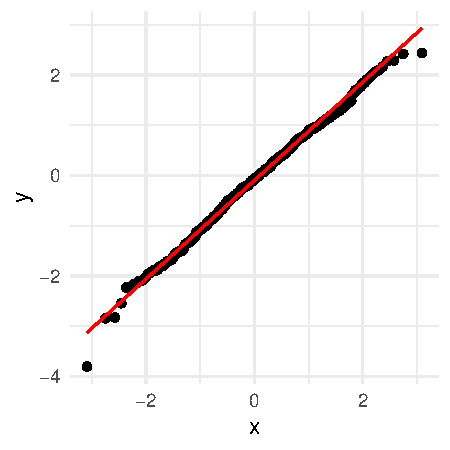
\includegraphics[width=\maxwidth]{img/mc-regression-05-a-1} 

}







\begin{enumerate}
\item [\textbf{A} \msquare] Die Annahme der normalverteilten Residuen ist erfüllt. Die Punkte liegen zum überwiegenden Teil nicht auf der Geraden und Korrelation ist negativ.
\item [\textbf{B} \msquare] Die Annahme der normalverteilten Residuen ist erfüllt. Die Punkte liegen zum überwiegenden Teil auf der Geraden.
\item [\textbf{C} \msquare] Die Annahme der normalverteilten Residuen ist erfüllt. Die Punkte liegen zum überwiegenden Teil nicht auf der Geraden.
\item [\textbf{D} \msquare] Wir betrachten insbesondere die beiden Enden der Gerade. Der Rest ist mehr oder minder egal, dann ist die Annahme an die Normalverteilung der Residuen erfüllt.
\item [\textbf{E} \msquare] Wir betrachten die Gerade. Wenn die Punkte einigermaßen gleichmäßig um die Gerade verteilt liegen, dann gehen wir von normalverteilten Residuen aus. Dies ist hier nicht der Fall. Wir haben keine normalverteilten Residuen vorliegen.
\end{enumerate}

\section{Aufgabe \hfill (2 Punkte)}

%% --------------------------------------------------------------------
\ifcollection
\begin{flushright}
\tiny\vspace{-2Ex}
\textbf{\examinhaltstart}
\exammodulestat $\;\bullet$
\exammodulestatbbv $\;\bullet$
\exammodulestatversuch $\;\bullet$
\exammodulebiostat
\vspace{-1Ex}
\end{flushright}
\fi
%% --------------------------------------------------------------------




In den Humanwissenschaften wird der Korrelationskoeffizienten $\rho$ sehr häufig verwendet. Daher ist es auch wichtig für andere Forschende den Korrelationskoeffizienten $\rho$ zu verstehen. Welche Aussazu zu dem Korrelationskoeffizienten $\rho$ ist richtig?




\begin{enumerate}
\item [\textbf{A} \msquare] Der Korrelationskoeffizienten $\rho$ ist eine veraltete Darstellungsform von Effekten in der linearen Regression und wird wie das $\eta^2$ aus der ANOVA interpretiert. Der Korrelationskoeffizienten $\rho$ beschreibt den Anteil an erklärter Varianz durch die Regression.
\item [\textbf{B} \msquare] Korrelationskoeffizienten $\rho$ liegt zwischen 0 und 1. Darüber hinaus ist der Korrelationskoeffizienten $\rho$ einheitslos und kann als Standardisierung verstanden werden.
\item [\textbf{C} \msquare] Der Korrelationskoeffizienten $\rho$ wird wie das $\eta^2$ aus der ANOVA interpretiert. Der Korrelationskoeffizienten $\rho$ beschreibt den Anteil an erklärter Varianz durch die Regression. Dabei gibt er jedoch eine Richtung an und kann auch negativ werden.
\item [\textbf{D} \msquare] Der Korrelationskoeffizienten $\rho$ zeigt keinen Zusammenhang zwischen zwei Variablen $x$ und $y$ bei einem Wert von 0. Einen negativen Zusammenhang Richtung -1 und somit auch einen positiven Zusammenhang Richtung 1. Je größer die Zahl allgemein, desto stärker der Effekt.
\item [\textbf{E} \msquare] Der Korrelationskoeffizienten $\rho$ zeigt keinen Zusammenhang zwischen zwei Variablen $x$ und $y$ bei einem Wert von 0. Einen maximalen negativen Zusammenhang bei -1 und somit auch einen maximalen positiven Zusammenhang bei 1. Korrelationskoeffizienten $\rho$ ist einheitslos.
\end{enumerate}

\section{Aufgabe \hfill (2 Punkte)}

%% --------------------------------------------------------------------
\ifcollection
\begin{flushright}
\tiny\vspace{-2Ex}
\textbf{\examinhaltstart}
\exammodulestatversuch $\;\bullet$
\exammodulebiostat
\vspace{-1Ex}
\end{flushright}
\fi
%% --------------------------------------------------------------------




Sie rechnen eine linearen Regression und erhalten folgende Abbildung der Residuen (\texttt{.resid}). Welche Aussage ist richtig?



{\centering 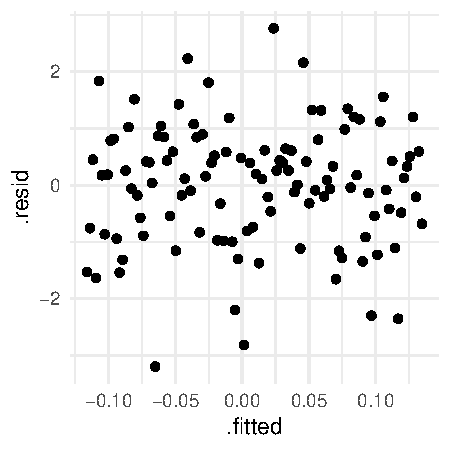
\includegraphics[width=\maxwidth]{img/mc-regression-06-a-1} 

}







\begin{enumerate}
\item [\textbf{A} \msquare] Wenn wir die Nulllinie betrachten so müssen die Punkte gleichmäßig unter der Nulllinie liegen. Unser Modell erfüllt somit nicht die Annahme von normalverteilten Residuen mit einem Mittelwert von $>0$ und einer Streuung von $s$.
\item [\textbf{B} \msquare] Die Annahme der normalverteilten Residuen ist nicht erfüllt. Vereinzelte Punkte liegen oberhalb bzw. unterhalb der Geraden um die 0 Linie weiter entfernt. Ein klares Muster ist zu erkennen.
\item [\textbf{C} \msquare] Wir betrachten die Nulllinie und alle Punkte sollten ohne Muster gleichmäßig um die Nulllinie liegen. Da dies der Fal ist, gehen wir von keinen Ausreißern aus.
\item [\textbf{D} \msquare] Die Annahme der normalverteilten Residuen ist erfüllt. Die Punkte liegen zum überwiegenden Teil auf der Diagonalen. Damit ist das Modell erfolgreich geschätzt worden.
\item [\textbf{E} \msquare] Die Annahme der normalverteilten Residuen ist nicht erfüllt. Ein klares Muster ist zu erkennen und/oder einige Outlier sind zu beobachten.
\end{enumerate}

\section{Aufgabe \hfill (2 Punkte)}

%% --------------------------------------------------------------------
\ifcollection
\begin{flushright}
\tiny\vspace{-2Ex}
\textbf{\examinhaltstart}
\exammodulebiostat
\vspace{-1Ex}
\end{flushright}
\fi
%% --------------------------------------------------------------------




Nach einer simplen linearen Regression zur Untersuchung vom Einfluss der $PO_2$-Konzentration in [$\mu g$] im Wasser auf das Trockengewicht von Erbsen in [$kg$] erhalten Sie einen $\beta_{PO_2}$ Koeffizienten von $6.9\times 10^{-7}$ und einen hoch signifikanten $p$-Wert mit $1e-04$. Warum sehen Sie so einen kleinen Effekt bei einer so deutlichen Signifikanz?




\begin{enumerate}
\item [\textbf{A} \msquare] Die Einheit der $PO_2$-Konzentration ist zu klein gewählt. Dadurch sehen wir den sehr kleinen $p$-Wert. Der $p$-Wert und die Einheit von der $PO_2$-Konzentration hängen antiproportional zusammen.
\item [\textbf{B} \msquare] Wenn der Effekt $\beta_{PO_2}$ sehr klein ist, dann kann es an einer falsch gewählten Einheit liegen. Der Anstieg von einer Einheit in $X$ führt ja zu einer Änderung von $\beta_{PO_2}$ in $y$. Daher ist hier mit einer anderen Einheit in den Daten zu rechnen, so dass wir hier einen besser formatierten Effekt sehen. Der p-Wert stammt aus einer einheitslosen Teststatistik.
\item [\textbf{C} \msquare] Manchmal ist die Einheit der Einflussvariable $X$ zu groß gewählt, so dass der Ansteig von 1 Einheit in $X$ zu einer zu großen Änderung in $y$ führt. Daher kann der Effekt $\beta_{PO_2}$ sehr klein wirken, da der p-Wert wird auf einer einheitslosen Teststatistik bestimmt wird.
\item [\textbf{D} \msquare] Das Gewicht und die $PO_2$-Konzentration korrelieren sehr stark, deshalb wird der $\beta_{PO_2}$ Koeffizient sehr klein. Mit einer ANOVA kann für die Korrelation korrigiert werden und der Effektschätzer passt dann zum p-Wert.
\item [\textbf{E} \msquare] Die Fallzahl ist zu hoch angesetzt. Je höher die Fallzahl ist, desto kleiner ist die Teststatistik und damit ist dann auch der $p$-Wert sehr klein. Es sollte über eine Reduzierung der Fallzahl nachgedacht werden. Dann sollte der Effekt zum p-Wert passen.
\end{enumerate}

\section{Aufgabe \hfill (2 Punkte)}

%% --------------------------------------------------------------------
\ifcollection
\begin{flushright}
\tiny\vspace{-2Ex}
\textbf{\examinhaltstart}
\exammodulestatversuch $\;\bullet$
\exammodulebiostat
\vspace{-1Ex}
\end{flushright}
\fi
%% --------------------------------------------------------------------




Nachdem Sie Ihr Experiment abgeschlossen haben, stehen Sie vor der Frage wie Sie Ihre Daten modellieren sollen. In der Beispielauswertung von Ihrem Betreuenden finden Sie die Funktion \texttt{lm()} in \Rlogo. Welche Aussage ist richtig?





\begin{enumerate}
\item [\textbf{A} \msquare] Die Funktion \texttt{lm()} in \Rlogo wird klassischerweise für die nicht-lineare Regression genutzt. Ist die Einflussvariable $X$ numerisch so werden die Gruppenmittelwerte geschätzt.
\item [\textbf{B} \msquare] Die Funktion \texttt{lm()} in \Rlogo ist der letzte Schritt für einen Gruppenvergleich. Vorher kann eine ANOVA oder aber ein multipler Vergleich in \{emmeans\} gerechnet werden. In der Funktion  \texttt{lm()} werden die Gruppenvarianzen bestimmt.
\item [\textbf{C} \msquare] Die Funktion \texttt{lm()} in \Rlogo ist der erste Schritt für einen Gruppenvergleich. Danach kann eine ANOVA oder aber ein multipler Vergleich in \{emmeans\} gerechnet werden. In der Funktion  \texttt{lm()} werden die Gruppenmittelwerte bestimmt.
\item [\textbf{D} \msquare] Die Funktion \texttt{lm()} berechnet die Varianzstruktur für eine ANOVA. Dannach kann dann über eine explorative Datenalayse nochmal eine Signifikanz berechnet werden. Sollte vor der Verwendung der Funktion \texttt{lm()} schon eine EDA gerechnet worden sein, so ist die Analyse wertlos.
\item [\textbf{E} \msquare] Ist die Einflussvariable $X$ numerisch so werden die Gruppenmittelwerte geschätzt und eine anschließende ANOVA sowie multipler Gruppenvergleich mit \{emmeans\} ist möglich.
\end{enumerate}

\section{Aufgabe \hfill (2 Punkte)}

%% --------------------------------------------------------------------
\ifcollection
\begin{flushright}
\tiny\vspace{-2Ex}
\textbf{\examinhaltstart}
\exammodulebiostat
\vspace{-1Ex}
\end{flushright}
\fi
%% --------------------------------------------------------------------




Welche Aussage über das \textit{generalisierte lineare Modell (GLM)} ist richtig?




\begin{enumerate}
\item [\textbf{A} \msquare] Das GLM erlaubt auch nicht normalverteilte Residuen in der Schätzung der Regressionsgrade.
\item [\textbf{B} \msquare] Das GLM ist ein faktisch maschineller Lernalgorithmus, der selstständig die Verteilungsfamilie für Y wählt.
\item [\textbf{C} \msquare] In \Rlogo ist mit dem \textit{generalisierten linearen Modell (GLM)} eine Modellierung implementiert, die die Poissonverteilung für Zähldaten oder die Binomialverteilung für 0/1-Daten modellieren kann. Weitere Modellierungen sind in \Rlogo auch mit zusätzlich geladenen Paketen nicht möglich.
\item [\textbf{D} \msquare] Das GLM ist eine allgemeine Erweiterung der linearen Regression auf die Normalverteilung.
\item [\textbf{E} \msquare] Das \textit{generalisierte lineare Modell (GLM)} erlaubt auch weitere Verteilungsfamilien für das $Y$ bzw. das Outcome in einer linearen Regression zu wählen.
\end{enumerate}

\section{Aufgabe \hfill (2 Punkte)}

%% --------------------------------------------------------------------
\ifcollection
\begin{flushright}
\tiny\vspace{-2Ex}
\textbf{\examinhaltstart}
\exammodulebiostat
\vspace{-1Ex}
\end{flushright}
\fi
%% --------------------------------------------------------------------




Sie führen ein Experiment zur Behandlung von Klaueninfektionen bei Schafe durch. Bei 3 Tieren finden Sie eine Erkrankung der Klauen vor und 12 Tiere sind gesund. Welche Aussage über den Effektschätzer Risk ratio ist richtig?



\begin{enumerate}
\item [\textbf{A} \msquare] Es ergibt sich ein Risk ratio von 0.25, da es sich um ein Anteil handelt.
\item [\textbf{B} \msquare] Der Anteil der Gesunden wird berechnet. Da es sich um ein Anteil handelt ergibt sich ein Risk ratio von 0.2.
\item [\textbf{C} \msquare] Das Verhältnis von Chancen Risk ratio ergibt ein Chancenverhältnis von 0.25.
\item [\textbf{D} \msquare] Da es sich um ein Chancenverhältnis handelt ergibt sich ein Risk ratio von 5.
\item [\textbf{E} \msquare] Das Verhältnis der Anteile Risk ratio ergibt ein Anteilsverhältnis von 0.2. Wir sind am Anteil der Kranken interessiert.
\end{enumerate}
    
% -----------------------------------------------------------------------
\clearpage
% -----------------------------------------------------------------------
\part{Programmieren in R}
% -----------------------------------------------------------------------

\section{Aufgabe \hfill (9 Punkte)}



 
%% --------------------------------------------------------------------
\ifcollection
\begin{flushright}
\tiny\vspace{-3Ex}
\textbf{\examinhaltstart}
\exammodulemathstat $\;\bullet$
\exammodulestat 
\vspace{-4Ex}
\end{flushright}
\begin{minipage}[t]{0.5\textwidth}

\includegraphics[width = 1.3cm]{/Users/kruppajo/work/GitHub/exam/avatare/Yuki.png}
\end{minipage}
\begin{minipage}[t]{0.5\textwidth}
\hfill
\href{https://www.youtube.com/playlist?list=PLe51bCp9JvEFUnFqaJG5aRmON9i1ZbOYC}{
\includegraphics[width = 2cm]{img/youtube}}
\end{minipage}
\vspace{-3ex}
\fi
%% --------------------------------------------------------------------



\ifcollection
\paragraph{Grundlegende Kenntnisse der Programierung in \Rlogo}
\fi

'Hm. \Rlogo ist eigentlich gar nicht so schwer, wenn man die Grundlagen kann.', meint  Yuki ganz zuversichtlich. Nur leider kennt er sich überhaupt nicht mit \Rlogo aus! Das heißt, Sie müssen hier einmal Rede und Antwort stehen und helfen.\\[1Ex]

Yuki: \textit{Jetzt sehe ich wieder diese Tilde ($\sim$) in R. Wo brauchen wir diese denn nochmal?} \textbf{(1 Punkt)}\\[1ex]
Sie antworten:\\[3Ex]

Yuki: \textit{Der Zuweisungs-Operator wird sehr häufig genutzt. Wie sieht der aus und wie funktioniert der an einem Beispiel?} \textbf{(1 Punkt)}\\[1ex]
Sie antworten:\\[3Ex]

Yuki: \textit{Wie heißen nochmal die beiden \Rlogo Pakete, die wir fast immer laden, wenn wir \Rlogo nutzen wollen?} \textbf{(1 Punkt)}\\[1ex]
Sie antworten:\\[3Ex]

Yuki: \textit{Warum gibt es eigentlich Objekte, Wörter und Funktionen in R? Wie unterscheiden sich diese überhaupt?} \textbf{(1 Punkt)}\\[1ex]
Sie antworten:\\[3Ex]

Yuki: \textit{Der Pipe-Operator wird sehr häufig genutzt. Wie sieht der aus und wie funktioniert der an einem Beispiel?} \textbf{(1 Punkt)}\\[1ex]
Sie antworten:\\[3Ex]

Yuki: \textit{Wie war nochmal der Name der Funktion in dem wir in R Daten intern abspeichern? Was waren da nochmal die Vorteile?} \textbf{(1 Punkt)}\\[1ex]
Sie antworten:\\[3Ex]

Yuki: \textit{Teilweise brauche ich das Konzept des Faktors in \Rlogo. Was ist ein Faktor?} \textbf{(1 Punkt)}\\[1ex]
Sie antworten:\\[3Ex]

Yuki: \textit{Was ist der Unterschied zwischen dem RStudio und R?} \textbf{(1 Punkt)}\\[1ex]
Sie antworten:\\[3Ex]

Yuki: \textit{Warum nutzen wir eigentlich dieses \texttt{c()} in \Rlogo?} \textbf{(1 Punkt)}\\[1ex]
Sie antworten:\\[3Ex] 
\clearpage
% -----------------------------------------------------------------------

\section{Aufgabe \hfill (9 Punkte)}



 
%% --------------------------------------------------------------------
\ifcollection
\begin{flushright}
\tiny\vspace{-3Ex}
\textbf{\examinhaltstart}
\exammodulestatversuch $\;\bullet$
\exammodulebiostat
\vspace{-4Ex}
\end{flushright}
\begin{minipage}[t]{0.5\textwidth}

\includegraphics[width = 1.3cm]{/Users/kruppajo/work/GitHub/exam/avatare/Jessica.png}
\end{minipage}
\begin{minipage}[t]{0.5\textwidth}
\hfill
\href{https://www.youtube.com/playlist?list=PLe51bCp9JvEFUnFqaJG5aRmON9i1ZbOYC}{
\includegraphics[width = 2cm]{img/youtube}}
\end{minipage}
\vspace{1ex}
\fi
%% --------------------------------------------------------------------



\ifcollection
\paragraph{Fortgeschrittene Kenntnisse der Programierung in \Rlogo}
\fi

'Hm...am Ende ist dann \Rlogo eigentlich gar nicht so schwer, wenn ich Hilfe habe.', meint  Jessica stolz und lacht Sie an. Nur leider kennt sie sich überhaupt nicht mit \Rlogo aus! Das heißt, Sie müssen hier einmal Rede und Antwort stehen und helfen. Sonst wird es für Jessica dann in ihrer Abschlussarbeit nichts mit der Auswertung und Abgabe. Das kann auch keine Lösung für Jessica und Sie sein. Immerhin haben Sie schon so viel gelernt.\\[1Ex]

Jessica fragt: \textit{Es gibt ja nur ein richtiges Format für die Eingabe eines Datums. Wie lautet das Format? \textbf{(1 Punkt)}}\\[1ex]
Sie antworten:\\[7Ex]

Jessica fragt: \textit{Oh, wie baue ich mir nochmal die Daten in R? Wie heißt das Dateiformat? Gerne einmal mit Beispiel! \textbf{(1 Punkt)}}\\[1ex]
Sie antworten:\\[7Ex]

Jessica fragt: \textit{Man kann doch die Funktion \texttt{emmeans()} von Varianzhomogenität auf Varianzheterogenität umstellen. Wie ging das noch gleich? \textbf{(1 Punkt)}}\\[1ex]
Sie antworten:\\[7Ex]

Jessica fragt: \textit{Ich will das R Paket \texttt{\{ggplot\}} nutzen, da war so eine Analogie an die ich mich nicht erinnern kann. Was war noch gleich das Prinzip von \texttt{\{ggplot\}}? Wie funktioniert \texttt{\{ggplot\}} konzeptionell? \textbf{(2 Punkte)}}\\[1ex]
Sie antworten:\\[7Ex]

Jessica fragt: \textit{Ich baue mir ja meinen Datensatz in Excel. Was muss ich da im Bezug auf die Namen der Spalten beachten? \textbf{(1 Punkt)}}\\[1ex]
Sie antworten:\\[7Ex]

Jessica fragt: \textit{Hm... wenn ich in R Daten mit Gruppen eingelesen habe, was muss ich dann nochmal als erstes machen? Und warum? \textbf{(2 Punkte)}}\\[1ex]
Sie antworten:\\[7Ex]

Jessica fragt: \textit{Welche Funktionen brauche ich in welcher Reihenfolge um eine ANOVA zu rechnen? \textbf{(1 Punkt)}}\\[1ex]
Sie antworten:\\[7Ex]



 
\clearpage
% -----------------------------------------------------------------------
\part{Deskriptive Statistik \& Explorative Datenanalyse}
% -----------------------------------------------------------------------

\section{Aufgabe \hfill (8 Punkte)}

\textit{Geben Sie grundsätzlich Formeln und Rechenweg zur Lösung der Teilaufgaben mit an!} \\[1Ex]
 

 
%% --------------------------------------------------------------------
\ifcollection
\begin{flushright}
\tiny\vspace{-3Ex}
\textbf{\examinhaltstart}
\exammodulemathstat $\;\bullet$
\exammodulestat $\;\bullet$
\exammodulestatbbv $\;\bullet$
\exammodulestatversuch $\;\bullet$
\exammodulebiostat
\vspace{-4Ex}
\end{flushright}
\begin{minipage}[t]{0.5\textwidth}

\includegraphics[width = 1.3cm]{/Users/kruppajo/work/GitHub/exam/avatare/Nilufar.png}
\end{minipage}
\begin{minipage}[t]{0.5\textwidth}
\hfill
\href{https://youtu.be/t0WYa_LVc5o}{
\includegraphics[width = 2cm]{img/youtube}}
\end{minipage}
\vspace{-3ex}
\fi
%% --------------------------------------------------------------------



\ifcollection
\paragraph{Zerforschen des Barplots}
\fi

Nilufar steht vor einem ersten Problem, denn wenn es nach ihrer Betreuer geht, soll sie in einem einem Feldexperiment Erbsen auswertet. Soweit eigentlich alles passend. Besser wäre was anderes gewesen. Hip Hop. Ein wunderbares Hobby um sich drin zu verlieren und Abstand zu bekommen. Nilufar denkt gerne über Hip Hop nach. Das heißt erstmal überlegen für Nilufar. Aus den Boxen wummert Deichkind und ihr Mund ist verklebt von Takis Blue Heat. 'Herrlich', denkt Nilufar. Die Behandlung werden verschiedene Lichtstufen ($none$, $200lm$ und $600lm$) sein. In ihrer Exceldatei wird sie den Outcome ($Y$) \textit{Ertrag} als \textit{yield} aufnehmen. Vorab soll Nilufar aber eimal die folgenden Barplots ihrer Betreuer nachbauen, damit sie den \Rlogo Code schonmal für später vorliegen hat. Damit geht das Problem schon los. Wenn die Erwartung nicht wäre, ja dann wäre wohl vieles möglich für Nilufar! Aber so..



{\centering 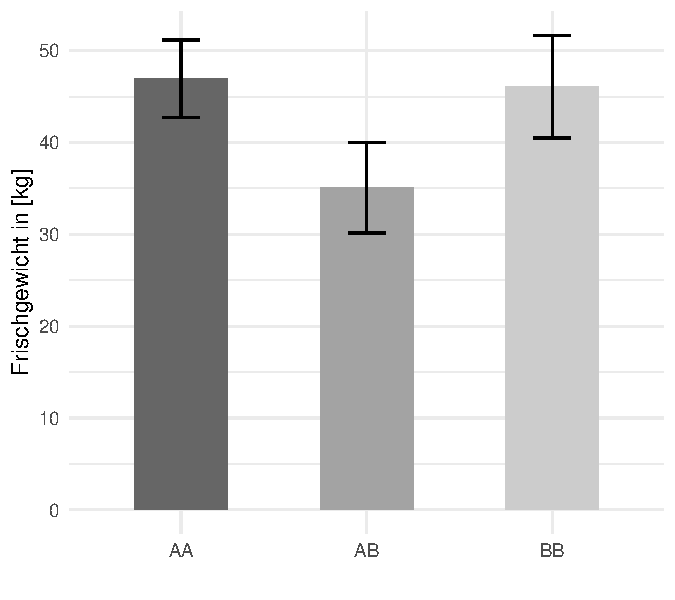
\includegraphics[width=\maxwidth]{img/barplot-02-1} 

}




Leider kennt sich Nilufar mit der Erstellung von Barplots in \Rlogo nicht aus. Deshalb braucht sie bei der Visualisierung Ihre Hilfe!

\begin{enumerate}
\item Formulieren Sie die wissenschaftliche Fragestellung! \textbf{(1 Punkt)}
\item Erstellen Sie eine Tabelle mit den statistischen Maßzahlen der drei Barplots! \textit{Beachten Sie die korrekte Darstellungsform der statistischen Maßzahlen!} \textbf{(3 Punkte)}
\item Erstellen Sie einen beispielhaften Datensatz im \Rlogo üblichen Format, aus dem die drei Barplots \textit{möglicherweise} erstellt wurden! \textbf{(2 Punkte)}
\item Kann Nilufar einen Unterschied zwischen den Behandlungen erwarten? Begründen Sie Ihre Antwort! \textbf{(2 Punkte)}
\end{enumerate} 
\clearpage
% -----------------------------------------------------------------------

\section{Aufgabe \hfill (8 Punkte)}

\textit{Geben Sie grundsätzlich Formeln und Rechenweg zur Lösung der Teilaufgaben mit an!} \\[1Ex]
 

 
%% --------------------------------------------------------------------
\ifcollection
\begin{flushright}
\tiny\vspace{-3Ex}
\textbf{\examinhaltstart}
\exammodulemathstat $\;\bullet$
\exammodulestat $\;\bullet$
\exammodulestatbbv 
\vspace{-4Ex}
\end{flushright}
\begin{minipage}[t]{0.5\textwidth}

\includegraphics[width = 1.3cm]{/Users/kruppajo/work/GitHub/exam/avatare/Steffen.png}
\end{minipage}
\begin{minipage}[t]{0.5\textwidth}
\hfill
\href{https://youtu.be/vXnLttRL_VI}{
\includegraphics[width = 2cm]{img/youtube}}
\end{minipage}
\vspace{-3ex}
\fi
%% --------------------------------------------------------------------



\ifcollection
\paragraph{Visualisierung des Barplots}
\fi

Steffen steht vor einem ersten Problem, denn wenn es nach seiner Betreuerin geht, soll er in einem einem Gewächshausexperiment Maiss auswertet. Soweit eigentlich alles passend. Besser wäre was anderes gewesen. Am Ende dann doch besser Klemmbausteine. Wunderbar. Eine echte Ablenkung für Steffen. Die Behandlung waren verschiedene Lichtstufen ($none$, $200lm$ und $600lm$). In seiner Exceldatei hat er den Messwert ($Y$) \textit{Ertrag} als \textit{yield} aufgenommen. Nun soll Steffen die Daten eimal als Barplots in einer Präsentation visualisieren, damit seiner Betreuerin wieder klar wird, was er eigentlich nochmal gemacht hat und was für ein Ergbnis in einem statistischen Test zu erwarten wäre. Wäre da nicht noch etwas. Steffen und die Romantik, eine unendliche Geschichte mit kniffeligen Wendungen. Aber egal. Um zu Ringen geht Steffen dann später nochmal raus. Echte Entspannung.

\begin{table}[!h]
\centering
\begin{tabular}{cc}
\toprule
treatment & yield\\
\midrule
200lm & 41.5\\
600lm & 31.3\\
none & 40.7\\
none & 25.6\\
none & 44.6\\
\addlinespace
200lm & 42.3\\
600lm & 21.7\\
600lm & 35.4\\
none & 32.1\\
200lm & 42.3\\
\addlinespace
600lm & 34.5\\
200lm & 44.0\\
none & 23.3\\
600lm & 37.1\\
200lm & 45.6\\
\bottomrule
\end{tabular}
\end{table}



Leider kennt sich Steffen mit der Erstellung von Barplots nicht aus. Deshalb braucht er bei der Visualisierung Ihre Hilfe!

\begin{enumerate}
\item Formulieren Sie die wissenschaftliche Fragestellung! \textbf{(1 Punkt)}
\item Zeichnen Sie in \textit{einer} Abbildung die Barplots für die Behandlung von Maiss! Beschriften Sie die Achsen entsprechend!\textbf{(4 Punkte)}
\item Beschriften Sie \textit{einen} Barplot mit den gängigen statistischen Maßzahlen! \textbf{(2 Punkte)}
\item Wenn Steffen \textit{keinen Effekt} zwischen den Behandlungen von Maiss erwarten würde, wie sehen dann die Barplots aus? \textit{Antworten Sie mit einer Skizze der Barplots!}
  \textbf{(1 Punkt)}
\end{enumerate} 
\clearpage
% -----------------------------------------------------------------------

\section{Aufgabe \hfill (9 Punkte)}

\textit{Geben Sie grundsätzlich Formeln und Rechenweg zur Lösung der Teilaufgaben mit an!} \\[1Ex]
 

 
%% --------------------------------------------------------------------
\ifcollection
\begin{flushright}
\tiny\vspace{-3Ex}
\textbf{\examinhaltstart}
\exammodulemathstat $\;\bullet$
\exammodulestat $\;\bullet$
\exammodulestatbbv $\;\bullet$
\exammodulestatversuch $\;\bullet$
\exammodulebiostat
\vspace{-4Ex}
\end{flushright}
\begin{minipage}[t]{0.5\textwidth}

\includegraphics[width = 1.3cm]{/Users/kruppajo/work/GitHub/exam/avatare/Tina.png}
\end{minipage}
\begin{minipage}[t]{0.5\textwidth}
\hfill
\href{https://youtu.be/Xf0yE-o7bEU}{
\includegraphics[width = 2cm]{img/youtube}}
\end{minipage}
\vspace{-3ex}
\fi
%% --------------------------------------------------------------------



\ifcollection
\paragraph{Zerforschen des Boxplots}
\fi

Tina steht vor einem ersten Problem, denn wenn es nach ihrer Betreuerin geht, soll sie in einem einem Versuch in einer Klimakammer Maiss auswertet. Soweit eigentlich alles passend. Besser wäre was anderes gewesen. Am Ende dann doch besser Astronomie. Wunderbar. Eine echte Ablenkung für Tina. Das heißt erstmal überlegen für Tina. Tina schmeißt noch eine Handvoll Katjes in ihren Rachen. Im Hintergrund klirrt leise der Spiegel zum Sound von Tocotronic. Die Behandlung werden verschiedene Bewässerungstypen ($low$, $mid$ und $high$) sein. In ihrer Exceldatei wird sie den Outcome ($Y$) \textit{Trockengewicht} als \textit{drymatter} aufnehmen. Vorab soll Tina aber eimal die folgenden Boxplots ihrer Betreuerin nachbauen, damit sie den \Rlogo Code schonmal für später vorliegen hat. Damit geht das Problem schon los. Tina und die Wut, eine unendliche Geschichte mit kniffeligen Wendungen.



{\centering 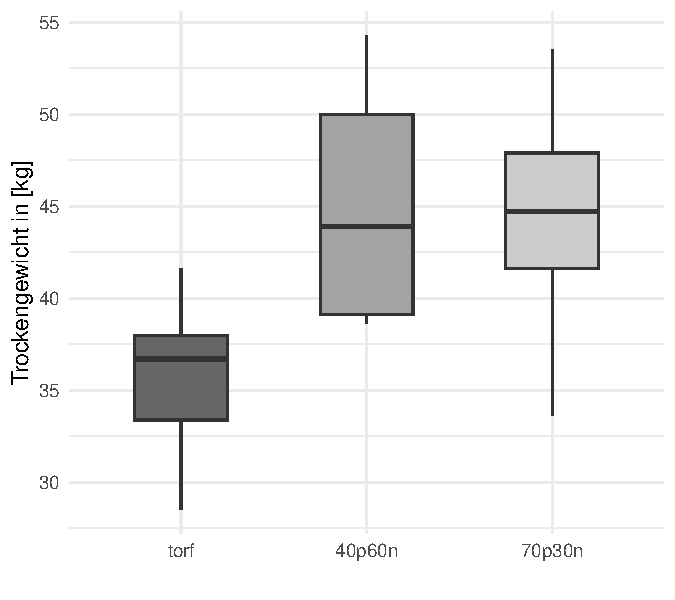
\includegraphics[width=\maxwidth]{img/boxplot-02-zer-1} 

}




Leider kennt sich Tina mit der Erstellung von Boxplots in \Rlogo nicht aus. Deshalb braucht sie bei der Visualisierung Ihre Hilfe!

\begin{enumerate}
\item Erstellen Sie eine Tabelle mit den statistischen Maßzahlen aus der obigen Abbildung der drei Boxplots! \textit{Beachten Sie die korrekte Darstellungsform der statistischen Maßzahlen!} \textbf{(3 Punkte)}
\item Beschriften Sie \textit{einen} der Boxplots mit den gängigen statistischen Maßzahlen! \textbf{(2 Punkte)}
\item Erstellen Sie einen beispielhaften Datensatz, aus dem die drei Boxplots \textit{möglicherweise} erstellt wurden, im \Rlogo üblichen Format! \textbf{(2 Punkte)}
\item Kann Tina einen Unterschied zwischen den Behandlungen erwarten? Begründen Sie Ihre Antwort! \textbf{(2 Punkte)}
\end{enumerate} 
\clearpage
% -----------------------------------------------------------------------

\section{Aufgabe \hfill (9 Punkte)}

\textit{Geben Sie grundsätzlich Formeln und Rechenweg zur Lösung der Teilaufgaben mit an!} \\[1Ex]
 

 
%% --------------------------------------------------------------------
\ifcollection
\begin{flushright}
\tiny\vspace{-3Ex}
\textbf{\examinhaltstart}
\exammodulemathstat $\;\bullet$
\exammodulestat $\;\bullet$
\exammodulestatbbv 
\vspace{-4Ex}
\end{flushright}
\begin{minipage}[t]{0.5\textwidth}

\includegraphics[width = 1.3cm]{/Users/kruppajo/work/GitHub/exam/avatare/Steffen.png}
\end{minipage}
\begin{minipage}[t]{0.5\textwidth}
\hfill
\href{https://youtu.be/0xc0jIPeiyw}{
\includegraphics[width = 2cm]{img/youtube}}
\end{minipage}
\vspace{-3ex}
\fi
%% --------------------------------------------------------------------



\ifcollection
\paragraph{Visualisierung des Boxplots}
\fi

Boxplots sind bedeutend in der Darstellung von wissenschaftlichen Ergebnissen. Leider hat sich Steffen nicht gemerkt, welche statistischen Maßzahlen für einen Boxplot erhoben werden müssen. Besser wäre was anderes gewesen. Klemmbausteine. Ein wunderbares Hobby um sich drin zu verlieren und Abstand zu bekommen. Steffen denkt gerne über Klemmbausteine nach. Das ist in soweit doof, da nach seinem Betreuer nun Boxplots aus seinen Daten gebaut werden sollen, bevor es mit dem statistischen Testen weitergeht. Anhand von Boxplots lässt sich eine Aussage über die Normalverteilung von $Y$ treffen. Die Behandlung für Erbsen waren verschiedene Genotypen ($AA$ und $BB$). Erfasst wurde von Steffen als Messwert ($Y$) \textit{Trockengewicht}. Steffen hat dann \textit{drymatter} in seiner Exceldatei eintragen. Aber nur in passender Atmospäre! Schon dutzende Male gesehen: Harry Potter. Aber immer noch großartig zusammen mit Oreos.

\begin{table}[!h]
\centering
\begin{tabular}{cc}
\toprule
treatment & drymatter\\
\midrule
AA & 34.9\\
AA & 35.4\\
BB & 40.1\\
BB & 28.1\\
BB & 34.1\\
\addlinespace
AA & 41.3\\
BB & 18.4\\
BB & 20.3\\
AA & 25.3\\
AA & 34.5\\
\addlinespace
AA & 20.1\\
AA & 21.1\\
AA & 39.6\\
BB & 27.4\\
AA & 25.7\\
\addlinespace
BB & 33.6\\
BB & 39.5\\
BB & 35.0\\
\bottomrule
\end{tabular}
\end{table}



Leider kennt sich Steffen mit der Erstellung von Boxplots nicht aus. Deshalb braucht er bei der Visualisierung Ihre Hilfe!

\begin{enumerate}
\item Zeichnen Sie in \textit{einer} Abbildung die beiden Boxplots für die zwei Behandlungen von Erbsen! Beschriften Sie die Achsen entsprechend! \textbf{(5 Punkte)} 
\item Wie ist Ihr Vorgehen, wenn Sie eine \textit{gerade} Anzahl an
  Beobachtungen pro Gruppe haben? \textbf{(1 Punkt)}
\item Beschriften Sie \textit{einen} der beiden Boxplots mit den gängigen
  statistischen Maßzahlen! \textbf{(2 Punkte)}
\item Wenn Sie \textit{keinen Effekt} zwischen den Behandlungen von
  Erbsen erwarten würden, wie sehen dann die beiden Boxplots aus?
  \textit{Antworten Sie mit einer Skizze der Boxplots!}
  \textbf{(1 Punkt)}
\end{enumerate} 
\clearpage
% -----------------------------------------------------------------------

\section{Aufgabe \hfill (8 Punkte)}

\textit{Geben Sie grundsätzlich Formeln und Rechenweg zur Lösung der Teilaufgaben mit an!} \\[1Ex]
 

 
%% --------------------------------------------------------------------
\ifcollection
\begin{flushright}
\tiny\vspace{-3Ex}
\textbf{\examinhaltstart}
\exammodulestatversuch $\;\bullet$
\exammodulebiostat
\vspace{-4Ex}
\end{flushright}
\begin{minipage}[t]{0.5\textwidth}

\includegraphics[width = 1.3cm]{/Users/kruppajo/work/GitHub/exam/avatare/Tina.png}
\end{minipage}
\begin{minipage}[t]{0.5\textwidth}
\hfill
\href{https://youtu.be/aXvxGC4YLqk}{
\includegraphics[width = 2cm]{img/youtube}}
\end{minipage}
\vspace{-3ex}
\fi
%% --------------------------------------------------------------------



\ifcollection
\paragraph{Visualisierung des Histogramm für kategoriale Daten}
\fi

Aus den Boxen wummert Tocotronic und ihr Mund ist verklebt von Katjes. 'Herrlich', denkt Tina. Tina betrachtet die folgenden Daten nach einem Stallexperiment mit Schweinen. In dem Experiment wurden die Anzahl an weißen Blutkörperchen gezählt. Nach der Meinung ihrem Betreuer muss als erstes geschaut werden, wie diese verteilt sind. Also welcher statistischen Verteilung die Anzahl an weißen Blutkörperchen folgen. Dazu soll Tina ein Histogramm verwenden. Dann hätte man auch einen guten Überblick über das Outcome ($Y$). Es wäre einfacher, wenn da nicht noch was wäre. Tina und die Wut, eine unendliche Geschichte mit kniffeligen Wendungen. Tina nickt im Takt von Tocotronic und bemerkt dabei gar nicht was die Spinne schon wieder anstellt.

\begin{center}
Die Anzahl an weißen Blutkörperchen: 3, 9, 4, 2, 2, 8, 3, 4, 4, 1, 6, 6, 3, 0, 5, 4, 1, 6, 5, 6, 5, 7, 2, 2, 5, 4, 2, 3, 1, 4, 4, 5, 3, 5, 5, 1
\end{center}

Leider kennt sich Tina mit der Erstellung von Histogrammen überhaupt nicht aus. Deshalb braucht sie bei der Erstellung Ihre Hilfe!

\begin{enumerate}
\item Zeichen Sie ein Histogramm um die Verteilung der Daten zu visualisieren! (\textbf{3 Punkte})
\item Beschriften Sie die Achsen der Abbildung! (\textbf{2 Punkte})
\item Ergänzen Sie die absoluten und relativen Häufigkeiten in der
  Abbildung! \textbf{(1 Punkt)}
\item Berechnen Sie aus den Daten die \textit{Wahrscheinlichkeit}
  gleich oder mehr als die Anzahl 6 zu beobachten! \textbf{(1
    Punkt)}
\item Berechnen Sie aus den Daten die \textit{Chance} gleich oder mehr
  als die Anzahl 6 zu beobachten! \textbf{(1 Punkt)}
\end{enumerate}

 
\clearpage
% -----------------------------------------------------------------------

\section{Aufgabe \hfill (8 Punkte)}

\textit{Geben Sie grundsätzlich Formeln und Rechenweg zur Lösung der Teilaufgaben mit an!} \\[1Ex]
 

 
%% --------------------------------------------------------------------
\ifcollection
\begin{flushright}
\tiny\vspace{-3Ex}
\textbf{\examinhaltstart}
\exammodulestatversuch $\;\bullet$
\exammodulebiostat
\vspace{-4Ex}
\end{flushright}
\begin{minipage}[t]{0.5\textwidth}

\includegraphics[width = 1.3cm]{/Users/kruppajo/work/GitHub/exam/avatare/Yuki.png}
\end{minipage}
\begin{minipage}[t]{0.5\textwidth}
\hfill
\href{https://youtu.be/ORHSPTCdfeY}{
\includegraphics[width = 2cm]{img/youtube}}
\end{minipage}
\vspace{-3ex}
\fi
%% --------------------------------------------------------------------



\ifcollection
\paragraph{Visualisierung des Histogramm für kontinuierliche Daten}
\fi

'Hm...', Reese's Peanut Butter Cups und London Grammar. Das ist und bleibt die beste Kombination zum Nachdenken für Yuki. Yuki betrachtet die folgenden Daten nach einem Versuch in einer Klimakammer mit Spargel. In dem Experiment wurden die mittleren Knötchen gezählt. Nach der Meinung seiner Betreuerin muss als erstes geschaut werden, wie diese verteilt sind. Also welcher statistischen Verteilung die mittleren Knötchen folgen. Dazu soll Yuki ein Histogramm verwenden. Dann hätte man auch einen guten Überblick über das Outcome ($Y$). Es wäre einfacher, wenn da nicht noch was wäre. Eine echte Herausforderung für ihn war schon immer die Faulheit gewesen. Ein leidiges Lied. Wenn London Grammar ertönt, dann sucht das Minischwein schleunigst Schutz unter dem Sofa. Yuki schüttelt den Kopf.

\begin{center}
Die mittleren Knötchen: 9.2, 9, 10.1, 10, 9, 7, 8.4, 10.4, 8.7, 12.8, 8.8, 15.1, 11.6, 11.5, 12.5, 11.9, 10.1, 10.1, 9.7, 6.9, 11.2, 8.7, 9.4, 7.2, 11.7, 10.7, 7.6, 11.3
\end{center}

Leider kennt sich Yuki mit der Erstellung von Histogrammen überhaupt nicht aus. Deshalb braucht er bei der Erstellung Ihre Hilfe!

\begin{enumerate}
\item Zeichen Sie ein Histogramm um die Verteilung der Daten zu visualisieren! (\textbf{3 Punkte})
 \item Erläutern Sie Ihr Vorgehen um ein Histogramm für kontinuierliche Daten zu zeichnen!  (\textbf{2 Punkte})
\item Beschriften Sie die Achsen der Abbildung! (\textbf{2 Punkte})
\item Ergänzen Sie die relativen Häufigkeiten in der Abbildung! \textbf{(1 Punkt)}  
\end{enumerate}

 
\clearpage
% -----------------------------------------------------------------------

\section{Aufgabe \hfill (10 Punkte)}

\textit{Geben Sie grundsätzlich Formeln und Rechenweg zur Lösung der Teilaufgaben mit an!} \\[1Ex]
 

 
%% --------------------------------------------------------------------
\ifcollection
\begin{flushright}
\tiny\vspace{-3Ex}
\textbf{\examinhaltstart}
\exammodulemathstat $\;\bullet$
\exammodulestat $\;\bullet$
\exammodulestatbbv $\;\bullet$
\exammodulestatversuch $\;\bullet$
\exammodulebiostat
\vspace{-4Ex}
\end{flushright}
\begin{minipage}[t]{0.5\textwidth}

\includegraphics[width = 1.3cm]{/Users/kruppajo/work/GitHub/exam/avatare/Jonas.png}
\end{minipage}
\begin{minipage}[t]{0.5\textwidth}
\hfill
\href{https://youtu.be/VAqiUdV4WQ0}{
\includegraphics[width = 2cm]{img/youtube}}
\end{minipage}
\vspace{-3ex}
\fi
%% --------------------------------------------------------------------




\ifcollection
\paragraph{Visualisierung des Scatterplots}
\fi

Wenn es nach Jonas ginge, wäre er schon längst fertig mit seiner Hausarbeit. Geht es aber nicht. Jonas schmeißt noch eine Handvoll Snickers in seinen Rachen. Im Hintergrund klirrt leise der Spiegel zum Sound von Iron Maiden. In seiner Hausarbeit hatte er ein Freilandversuch in der Uckermark durchgeführt. Nach der Meinung seiner Betreuerin sieht das jedoch etwas anders aus. Jetzt soll er doch noch eine explorative Datenanalyse für den Zusammenhang zwischen durschnittlichen Niederschlag [ml/w] und Trockengewicht [kg/ha] in Lauch durchführen. Wie nervig! Jonas und die Erschöpfung, eine unendliche Geschichte mit kniffeligen Wendungen. Da zwei kontinuierliche Variablen vorliegen, geht die explorative Datenanalyse leider nicht mit Boxplots oder Barplots. Dann was anderes. Wenn Mission Impossible läuft, dann ist das Meerschweinchen nicht mehr da. Aber jetzt braucht er mal Entspannung!

\begin{table}[!h]
\centering
\begin{tabular}{cc}
\toprule
Durschnittlichen Niederschlag [ml/w] & Trockengewicht [kg/ha]\\
\midrule
24.7 & 25.6\\
25.2 & 27.4\\
22.9 & 24.1\\
23.3 & 28.3\\
22.2 & 21.6\\
\addlinespace
24.5 & 28.6\\
26.7 & 31.5\\
28.7 & 27.3\\
25.1 & 27.1\\
24.2 & 26.9\\
\addlinespace
27.3 & 29.5\\
24.9 & 29.0\\
\bottomrule
\end{tabular}
\end{table}



Leider kennt sich Jonas mit der Erstellung einer explorativen Datenanalyse für kontinuierliche Daten überhaupt nicht aus. Deshalb braucht er bei der Erstellung Ihre Hilfe!

\begin{enumerate}
\item Erstellen Sie eine Visualisierung für die Datentabelle. Beschriften Sie
  die Achsen entsprechend! \textbf{(4 Punkte)}
\item Schätzen Sie eine Gerade durch die Punkte! \textbf{(1 Punkt)}
\item Beschriften Sie die Gerade mit den gängigen statistischen Maßzahlen! Geben Sie die numerischen Zahlenwerte mit an! \textbf{(3 Punkte)}
\item Wenn \textit{ein} Effekt von $x$ auf $y$ vorhanden wäre, wie würde die Gerade verlaufen und welche Werte würden die statistischen Maßzahlen annehmen? \textbf{(2 Punkt)}
\end{enumerate} 
\clearpage
% -----------------------------------------------------------------------

\section{Aufgabe \hfill (10 Punkte)}

\textit{Geben Sie grundsätzlich Formeln und Rechenweg zur Lösung der Teilaufgaben mit an!} \\[1Ex]
 

 
%% --------------------------------------------------------------------
\ifcollection
\begin{flushright}
\tiny\vspace{-3Ex}
\textbf{\examinhaltstart}
\exammodulestat $\;\bullet$
\exammodulestatbbv 
\vspace{-4Ex}
\end{flushright}
\begin{minipage}[t]{0.5\textwidth}

\includegraphics[width = 1.3cm]{/Users/kruppajo/work/GitHub/exam/avatare/Jessica.png}
\end{minipage}
\begin{minipage}[t]{0.5\textwidth}
\hfill
\href{https://youtu.be/t_1KL77mfmg}{
\includegraphics[width = 2cm]{img/youtube}}
\end{minipage}
\vspace{-3ex}
\fi
%% --------------------------------------------------------------------



\ifcollection
\paragraph{Visualisierung des Mosaicplots}
\fi

Zwei kategoriale Variablen darzustellen ist nicht so einfach. Jessica hatte erst über einen Mittelwert nachgedacht, dann aber die Idee verworfen. Wäre da nicht noch was anderes. Jessica und der Mangel, eine unendliche Geschichte mit kniffeligen Wendungen. Dabei hatte sie sich in einen Leistungssteigerungsversuch im Emsland zum einen die Behandlung Außenklimakontakt [ja/nein] und zum anderen die Messung Fettgehalt erreicht [ja/nein] im Kontext von Schweinen angeschaut. Jetzt möchte ihre Betreuerin erstmal die langen Tabellen mit ja/nein in einer explorativen Datenanalyse zusammengefasst bekommen. Sonst geht es bei ihrem Projektbericht nicht weiter. Was super nervig ist. Einfach mal raus um Rad zu fahren. Ohne Ziel und Uhr. Das ist was für Jessica.



\vspace{1Ex}

\begin{center}
\begin{minipage}[t]{0.45\textwidth}
%\small
\begin{center}

\begin{tabular}{p{2.5cm}p{2.5cm}p{2.5cm}p{2.5cm}}
\toprule
Außenklimakontakt & Fettgehalt erreicht\\
\midrule
nein & nein\\
ja & nein\\
ja & nein\\
nein & nein\\
nein & nein\\
\addlinespace
nein & nein\\
nein & nein\\
ja & ja\\
ja & nein\\
nein & nein\\
\addlinespace
ja & ja\\
nein & nein\\
nein & ja\\
nein & nein\\
nein & nein\\
\bottomrule
\end{tabular}


\end{center}
\end{minipage}
\begin{minipage}[t]{0.45\textwidth}
%\small
\begin{center}

\begin{tabular}{p{2.5cm}p{2.5cm}p{2.5cm}p{2.5cm}}
\toprule
Außenklimakontakt & Fettgehalt erreicht\\
\midrule
ja & nein\\
ja & nein\\
nein & nein\\
ja & ja\\
ja & nein\\
\addlinespace
nein & nein\\
ja & nein\\
ja & nein\\
nein & nein\\
nein & nein\\
\addlinespace
nein & nein\\
nein & nein\\
ja & nein\\
ja & nein\\
ja & nein\\
\bottomrule
\end{tabular}


\end{center}
\end{minipage}
\end{center}

\vspace{2Ex}

Leider kennt sich Jessica mit der Erstellung einer explorativen Datenanalyse für kategoriale Daten überhaupt nicht aus. Deshalb braucht sie bei der Erstellung Ihre Hilfe!

\begin{enumerate}
\item Stellen Sie den Zusammenhang zwischen den beiden kategorialen Variablen in einer zusammenfassenden Tabelle dar! \textbf{(3 Punkte)}
\item Visualisieren Sie den Zusammenhang zwischen den beiden kategorialen Variablen! \textbf{(3 Punkte)}
\item Berechnen Sie die Verhältnisse in der Visualisierung! Welche Annahme haben Sie getroffen? \textbf{(2 Punkte)}
\item Wenn \textit{ein} Effekt von der Behandlung vorliegen würde, wie würde die Tabelle und die Visualisierung aussehen? \textbf{(2 Punkt)}
\end{enumerate} 
\clearpage
% -----------------------------------------------------------------------

\section{Aufgabe \hfill (10 Punkte)}

\textit{Geben Sie grundsätzlich Formeln und Rechenweg zur Lösung der Teilaufgaben mit an!} \\[1Ex]
 

 
%% --------------------------------------------------------------------
\ifcollection
\begin{flushright}
\tiny\vspace{-3Ex}
\textbf{\examinhaltstart}
\exammodulestatversuch $\;\bullet$
\exammodulebiostat
\vspace{-4Ex}
\end{flushright}
\begin{minipage}[t]{0.5\textwidth}

\includegraphics[width = 1.3cm]{/Users/kruppajo/work/GitHub/exam/avatare/Jessica.png}\hspace{-4mm}
\includegraphics[width = 1.3cm]{/Users/kruppajo/work/GitHub/exam/avatare/Jonas.png}
\end{minipage}
\begin{minipage}[t]{0.5\textwidth}
\hfill
\href{https://youtu.be/Op-gjzASH9I}{
\includegraphics[width = 2cm]{img/youtube}}
\end{minipage}
\fi
%% --------------------------------------------------------------------



\ifcollection
\paragraph{Visualisierung von Verteilungen}
\fi

'Was hast du dir denn da hingeklebt? \textit{Frei ist, wer missfallen kann.}\footnote{Oschmann, A. (2024) Mädchen stärken: Stärken fördern, Selbstwert erhöhen und liebevoll durch Krisen begleiten. Goldegg Verlag}', liest Jessica vom Kühlschrank vor. Jessica und Jonas sitzen zusammen in der Küche und versuchen zu verhindern, dass die Hündin den Biomüll mampft. 'Können wir uns auf die etwas kryptische Aufgabe konzentrieren?', nöhlt Jonas. Die beiden schauen angestrengt auf die drei Boxplots. Das Ziel ist es zu verstehen, wie eine Verteilung anhand eines Boxplots bewertet werden kann. Jonas und die Erschöpfung machen die Sache nicht einfacher.



{\centering 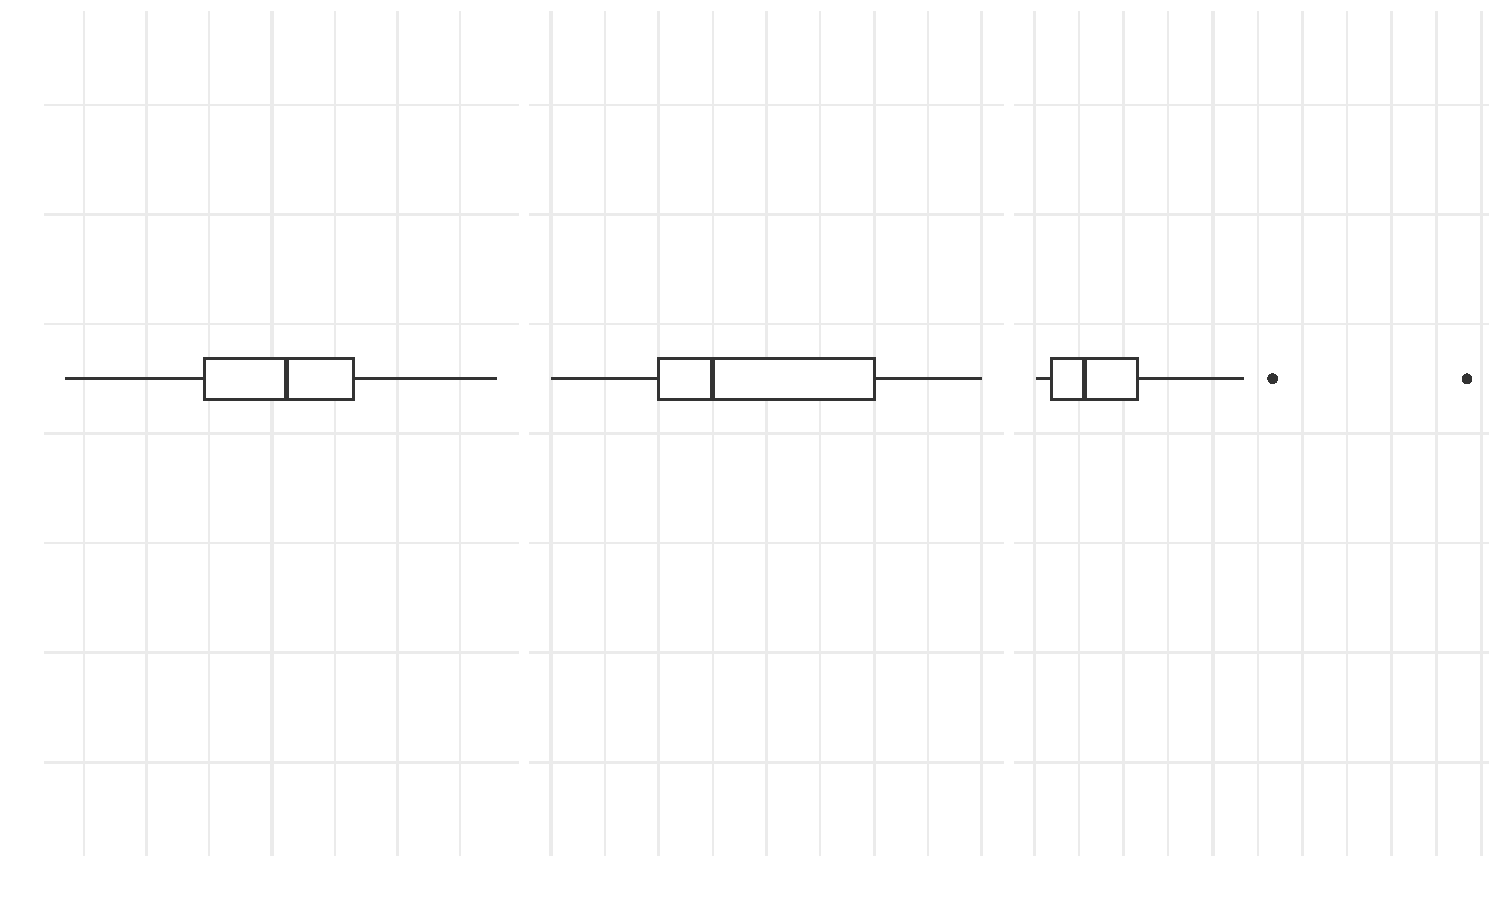
\includegraphics[width=\maxwidth]{img/desc-stat-11-1} 

}




Jetzt brauchen Jessica und Jonas Ihre Hilfe bei der Abschätzung einer Verteilung anhand von Boxplots um ihre Arbeit dann in diesem Semester noch abschließen zu können.

\begin{enumerate}
\item Zeichnen Sie über die Boxplots die entsprechende zugehörige Verteilung! \textbf{(3 Punkte)} 
\item Zeichnen Sie unter die Boxplots die entsprechende zugehörige Beobachtungen als Stiche! \textbf{(3 Punkte)}
\item Wie viel Prozent der Beobachtungen fallen in das IQR? Ergänzen Sie die Abbildung entsprechend um den Bereich! \textbf{(2 Punkte)}
\item Wie viel Prozent der Beobachtungen fallen in $\bar{y} \pm 1s$ und $\bar{y} \pm 2s$  unter der Annahme einer Normalverteilung? \textbf{(2 Punkte)}
\end{enumerate} 
\clearpage
% -----------------------------------------------------------------------
\part{Statistisches Testen \& statistische Testtheorie}
% -----------------------------------------------------------------------  

\section{Aufgabe \hfill (9 Punkte)}


 
%% --------------------------------------------------------------------
\ifcollection
\begin{flushright}
\tiny
\textbf{\examinhaltstart}
\exammodulestat $\;\bullet$
\exammodulestatbbv $\;\bullet$
\exammodulestatversuch $\;\bullet$
\exammodulebiostat
\vspace{-4Ex}
\end{flushright}
\begin{minipage}[t]{0.5\textwidth}
\includegraphics[width = 1.3cm]{/Users/kruppajo/work/GitHub/exam/avatare/Jonas.png}\hspace{-4mm}\includegraphics[width = 1.3cm]{/Users/kruppajo/work/GitHub/exam/avatare/Paula.png}
\end{minipage}
\begin{minipage}[t]{0.5\textwidth}
\hfill
\href{https://youtu.be/aHVYuFKTqZs}{\includegraphics[width = 2cm]{img/youtube}}
\end{minipage}
\fi
%% --------------------------------------------------------------------



\ifcollection
\paragraph{Grundgesamtheit und experimentelle Stichprobe}
\fi

'Grundlage des statistischen Testen ist das Verständnis von der Grundgesamtheit (eng. \textit{population} oder \textit{ground truth}) und der experimentellen Stichprobe (eng. \textit{sample}). ', liest Jonas laut aus dem Skript vor. Paula war kurz eingenickt und wird mit einem Stoß geweckt. 'Reiz dich zusammen und iss noch ein paar Snickers das hilft mir immer. Alleine komme ich hier nicht weiter.', tadelt Jonas Paula etwas zu forsch. 'War ne lange Nacht', mault Paula. Beide sollen in ihrer Abschlussarbeit einen statistischen Test interpretieren und versuchen die Grundlagen zu wiederholen. Paula war auf einem Konzert von White Lies.

\vspace{1ex}

Leider kennen sich Jonas und Paula mit der Grundgesamtheit und der Stuchprobe überhaupt nicht aus. Daher sind Sie gefragt!

\begin{enumerate}
\item Nennen Sie das statistische Verfahren und zwei konkrete Beispiele zur Durchführung um von einer Grundgesamtheit auf eine Stichprobe zu gelangen! \textbf{(3 Punkte)}
\item Erklären Sie den Zusammenhang zwischen Stichprobe und Grundgesamtheit an einem Schaubild! Beschriften Sie das Schaubild entsprechend!
  \textit{Nutzen Sie hierfür als Veranschaulichung ein aussagekräftiges Beispiel!}  \textbf{(3 Punkte)}
\item Erweitern Sie das Schaubild um die Entstehung von $Pr(D|H_0)$! \textit{Nutzen Sie hierfür als Veranschaulichung ein aussagekräftiges Beispiel!}  \textbf{(3 Punkte)}
\end{enumerate} 
\clearpage
% -----------------------------------------------------------------------

\section{Aufgabe \hfill (9 Punkte)}


 
%% --------------------------------------------------------------------
\ifcollection
\begin{flushright}
\tiny
\textbf{\examinhaltstart}
\exammodulestat $\;\bullet$
\exammodulestatbbv $\;\bullet$
\exammodulestatversuch $\;\bullet$
\exammodulebiostat
\vspace{-4Ex}
\end{flushright}
\begin{minipage}[t]{0.5\textwidth}
\includegraphics[width = 1.3cm]{/Users/kruppajo/work/GitHub/exam/avatare/Alex.png}\hspace{-4mm}\includegraphics[width = 1.3cm]{/Users/kruppajo/work/GitHub/exam/avatare/Steffen.png}
\end{minipage}
\begin{minipage}[t]{0.5\textwidth}
\hfill
\href{https://youtu.be/Ric8ne39DtI}{\includegraphics[width = 2cm]{img/youtube}}
\end{minipage}
\fi
%% --------------------------------------------------------------------



\ifcollection
\paragraph{Das Nullritual - Die statistische Testtheorie}
\fi

'Alien ist der beste Film, den es gibt.', meint Alex. Steffen entgegnet, ' Ich empfehle ja immer allen Harry Potter.'Die beiden sind im Zoo und diskutieren, ob Pinguine Knie haben. Eigentlich wollten beide nochmal die statistische Testheorie durchgehen, sind dann aber auf abenteuerlichen Wege im Zoo gelandet. Alex starrt wie hypnotisiert auf einen strullenden Elefanten und stopt die Zeit.\footnote{Yang, P. J., et al. (2014). Duration of urination does not change with body size. Proceedings of the National Academy of Sciences, 111(33), 11932-11937.} 'Du bist so peinlich.', entfährt es Steffen und schmeißt sich noch ein paar überteuerte Oreos rein.

\vspace{1ex}

Leider kennen sich Alex und Steffen mit statistischen Testtheorie, auch Null-Ritual genannt, überhaupt nicht aus. Geschweige denn mit der Visualisierung als Kreuztabelle.  

\begin{enumerate}
\item Tragen Sie folgende statistische Fachbegriffe zur statistischen Testtheorie korrekt eine selbst erstellte Kreuztabelle ein! \textbf{(3 Punkte)}
  \begin{center}
  \begin{tabular}{cccc}
  H$_0$ abgelehnt & H$_0$ falsch & H$_0$ beibehalten & H$_0$ wahr \\
  \end{tabular}
  \end{center}
\item Ergänzen Sie Ihre erstellte Kreuztabelle um vier weitere, passende Fachbegriffe zur statistischen Testtheorie! \textbf{(2 Punkte)}
\end{enumerate}

Die Entscheidungsfindung durch einen statistischen Test kann auch durch die Analogie zu einem Feuermelder abgebildet werden. Dabei symbolisiert der Feuermelder den statistischen Test und es soll getestet werden, ob ein Feuer ausgebrochen ist.

\begin{enumerate}
  \setcounter{enumi}{2}    
\item In der Analogie des Feuermelders, wie lautet der $\alpha$-Fehler? \textbf{(1 Punkt)}
\item In der Analogie des Feuermelders, wie lautet der $\beta$-Fehler? \textbf{(1 Punkt)}
\item Wenn der Feuermelder einmal pro Tag messen würde, wie oft würde der Feuermelder mit einem $\alpha$ von 5\% in einem Monat Alarm schlagen? Begründen Sie Ihre Antwort! \textbf{(2 Punkte)}
\end{enumerate}



 
\clearpage
% -----------------------------------------------------------------------

\section{Aufgabe \hfill (9 Punkte)}

\textit{Geben Sie grundsätzlich Formeln und Rechenweg zur Lösung der Teilaufgaben mit an!} \\[1Ex]


 
%% --------------------------------------------------------------------
\ifcollection
\begin{flushright}
\tiny\vspace{-3Ex}
\textbf{\examinhaltstart}
\exammodulemathstat $\;\bullet$
\exammodulestat $\;\bullet$
\exammodulestatbbv $\;\bullet$
\exammodulestatversuch $\;\bullet$
\exammodulebiostat
\vspace{-4Ex}
\end{flushright}
\begin{minipage}[t]{0.5\textwidth}
\includegraphics[width = 1.3cm]{/Users/kruppajo/work/GitHub/exam/avatare/Mark.png}\hspace{-4mm}\includegraphics[width = 1.3cm]{/Users/kruppajo/work/GitHub/exam/avatare/Paula.png}
\end{minipage}
\begin{minipage}[t]{0.5\textwidth}
\hfill
\href{https://youtu.be/32JjH1eyuTU}{\includegraphics[width = 2cm]{img/youtube}}
\end{minipage}
\fi
%% --------------------------------------------------------------------



\ifcollection
\paragraph{Visualisierung der Teststatistik $\boldsymbol{T_D}$ und dem p-Wert}
\fi

'Wir sollen die Teststatistik $T_D$ umd dem p-Wert visualisieren, da mit einer Visualisierung vieles verständlicher wird!', ruft Mark um Andrea Berg zu übertönen. 'Ich weiß nicht, was das jetzt helfen soll. Können wir nicht einfach schauen, ob der p-Wert kleiner als das Signifikanzniveau  $\alpha$ gleich 5\% ist? Und gut ist?', merkt Paula an, was aber im Refrain von Andrea Berg untergeht. Mark nickt im Beat. 'Wir haben hier eine t-verteilung unter der Annahme der Nullhypothese!', singt er.

\vspace{1ex}

Leider kennen sich Mark und Paula mit der Visualisierung der Teststatistik $T_D$ und dem p-Wert überhaupt nicht aus und brauchen dahr Ihre Hilfe!

\vspace{1ex}

\textit{Beachten Sie, dass im Folgenden \underline{keine numerisch korrekte Darstellung} verlangt wird! Es gilt Erkennbarkeit vor Genauigkeit!}

\begin{enumerate}
\item Ergänzen Sie eine beschriftete $x$-Achse! \textbf{(1 Punkt)}
\item Ergänzen Sie "`$\bar{y}_1 = \bar{y}_2$"'! \textbf{(1 Punkt)} 
\item Ergänzen Sie "`$A = 0.95$"'! \textbf{(1 Punkt)}
\item Zeichnen Sie $T_{\alpha=5\%}$ in die Abbildung! \textbf{(1 Punkt)} 
\item Zeichnen Sie das Signifikanzniveau $\alpha$ in die Abbildung! Begründen Sie Ihre Antwort! \textbf{(2 Punkte)} 
\item Zeichnen Sie $-T_{D}$ in die Abbildung! \textbf{(1 Punkt)}
\item Zeichnen Sie einen nicht signifikant p-Wert in die Abbildung! Begründen Sie Ihre Antwort! \textbf{(2 Punkte)}   
\end{enumerate}



{\centering \includegraphics[width=\maxwidth]{img/statistisches-testen-3-1} 

}


 
\clearpage
% -----------------------------------------------------------------------

\section{Aufgabe \hfill (10 Punkte)}


 
%% --------------------------------------------------------------------
\ifcollection
\begin{flushright}
\tiny
\textbf{\examinhaltstart}
\exammodulestatversuch $\;\bullet$
\exammodulebiostat
\vspace{-4Ex}
\end{flushright}
\begin{minipage}[t]{0.5\textwidth}
\includegraphics[width = 1.3cm]{/Users/kruppajo/work/GitHub/exam/avatare/Paula.png}\hspace{-4mm}\includegraphics[width = 1.3cm]{/Users/kruppajo/work/GitHub/exam/avatare/Steffen.png}
\end{minipage}
\begin{minipage}[t]{0.5\textwidth}
\hfill
\href{https://youtu.be/CN_O4fYPbhs}{\includegraphics[width = 2cm]{img/youtube}}
\end{minipage}
\fi
%% --------------------------------------------------------------------



\ifcollection
\paragraph{Visualisierung des 95\% Konfidenzintervalls}
\fi

'So, was haben wir gemacht? Wir haben einen t-test für den Vergleich der Mittelwerte gerechnet.', meint Steffen. Paula schaut fragend. 'Hatten wir nicht alles zu einer Kontrolle verglichen? Das war doch so!', ruft Paula laut aus. 'Wir haben doch als Messwert \textit{Energieverbrauch der Klimakammer} erhoben.', stellt Steffen fest. Jetzt haben beide das Problem, die möglichen 95\% Konfidenzintervalle zu interpretieren.

\vspace{1ex}

Leider kennen sich Steffen und Paula mit der Visualisierung des 95\% Konfidenzintervall überhaupt nicht aus. 

\begin{enumerate}
\item Beschriften Sie die untenstehende Abbildung mit der Signifikanzschwelle! Begründen Sie Ihre Antwort! \textbf{(2 Punkte)}
\item Ergänzen Sie eine \textit{in den Kontext passende} Relevanzschwelle! Begründen Sie Ihre Antwort! \textbf{(2 Punkte)} 
\item Skizieren Sie in die untenstehende Abbildung sechs einzelne Konfidenzintervalle (a-f) mit den
  jeweiligen Eigenschaften! \textbf{(6 Punkte)}
  \begin{itemize}
  \item[(a)] Ein 95\% Konfidenzintervall mit h{"o}herer Fallzahl $n$ in der Stichprobe als der Rest der 95\% Konfidenzintervalle 	
  \item[(b)] Ein signifikantes, relevantes 90\% Konfidenzintervall. 	
  \item[(c)] Ein signifikantes, relevantes 95\% Konfidenzintervall 	
  \item[(d)] Ein nicht signifikantes, nicht relevantes 95\% Konfidenzintervall 
  \item[(e)] Ein 95\% Konfidenzintervall mit niedriger Fallzahl $n$ in der Stichprobe als der Rest 95\% der Konfidenzintervalle
  \item[(f)] Ein signifikantes, nicht relevantes 95\% Konfidenzintervall
  \end{itemize}
\end{enumerate}

\begin{center}
  \includegraphics[height = 10cm]{/Users/kruppajo/work/GitHub/exam/question/img/statistisches-testen-04}
\end{center}


 
\clearpage
% -----------------------------------------------------------------------

\section{Aufgabe \hfill (10 Punkte)}

\textit{Geben Sie grundsätzlich Formeln und Rechenweg zur Lösung der Teilaufgaben mit an!} \\[1Ex]


 
%% --------------------------------------------------------------------
\ifcollection
\begin{flushright}
\tiny\vspace{-3Ex}
\textbf{\examinhaltstart}
\exammodulestatversuch $\;\bullet$
\exammodulebiostat
\vspace{-4Ex}
\end{flushright}
\begin{minipage}[t]{0.5\textwidth}
\includegraphics[width = 1.3cm]{/Users/kruppajo/work/GitHub/exam/avatare/Tina.png}\hspace{-4mm}\includegraphics[width = 1.3cm]{/Users/kruppajo/work/GitHub/exam/avatare/Yuki.png}
\end{minipage}
\begin{minipage}[t]{0.5\textwidth}
\hfill
\href{https://youtu.be/FgZmpnEWDag}{\includegraphics[width = 2cm]{img/youtube}}
\end{minipage}
\fi
%% --------------------------------------------------------------------



\ifcollection
\paragraph{Zusammenhang zwischen dem Effekt, der Streuung sowie der Fallzahl}
\fi

An einem heißen Juliabend haben sich Tina und Yuki zum Lernen verabredet. Eine große Kanne Eistee und Berge von Katjes schmelzen in der Sonne  und warten darauf gegessen zu werden. Tina liest laut vor:\begin{quote}
                 \textit{
                 Beim statistischen Testen gibt es einen Zusammenhang zwischen dem Effekt, der Streuung sowie der Fallzahl. Gegeben sei die Formel für den Student t-Test auf den die folgenden Überlegungen basieren sollen. Welche Auswirkung hat die Änderungen der jeweiligen statistischen Maßzahl des Effekts $\Delta$, der Streuung $s$ und der Fallzahl $n$ auf die Teststistik $T_{D}$, den p-Wert $Pr(D|H_0)$ sowie dem Konfidenzintervall $KI_{1-\alpha}$?
                 }
                 \end{quote}Yuki hebt die Augenbraue. 'Ich bleibe dabei. Wir sollten erstmal Matrix schauen, bis es kühler ist. Den Film habe ich doch extra mitgebracht!' Tina ist der Idee nicht abgeneigt und auch die Spinne kommt auf die Terasse um dabei zu sein.

\vspace{1ex}

Leider kennen sich Tina und Yuki mit dem Zusammenhang zwischen dem Effekt, der Streuung sowie der Fallzahl überhaupt nicht aus. 


\begin{enumerate}
\item Visualisieren Sie den Zusammenhang zwischen der Teststatiatik $T_{D}$ und dem p-Wert $Pr(D|H_0)$ für sich verändernde $T_{D}$-Werte!\textit{Geben Sie dafür ein numerisches Beispiel in dem Sie drei $T_{D}$-Werte und deren Einfluss auf den p-Wert vergleichen!} \textbf{(3 Punkte)}  
\item  Füllen Sie die untenstehende Tabelle aus in dem Sie die Änderung der statistischen Maßzahlen auf die Teststatistik, den p-Wert sowie das Konfidenzintervall in \textit{einem} Wort oder Symbol beschreiben! \textbf{(4 Punkte)}
\begin{center}
  \large
  \begin{tabular}[c]{l|c|c|c|l|c|c|c}
    & $T_{D}$ & $Pr(D|H_0)$ & $KI_{1-\alpha}$ & & $T_{D}$ & $Pr(D|H_0)$ & $KI_{1-\alpha}$\strut\\ 
    \hline
    \textbf{$\Delta\; \uparrow$} & \hspace{1.8cm} & \hspace{1.8cm}  & \hspace{1.8cm} & \textbf{
                                                          $\Delta\; \downarrow$} &
                                                                          \hspace{1.8cm} & \hspace{1.8cm}  & \hspace{1.8cm}\strut\\
    \hline
        \textbf{$s\; \uparrow$} & \hspace{1.8cm} & \hspace{1.8cm}  & \hspace{1.8cm} & \textbf{
                                                          $s\; \downarrow$} &
                                                                          \hspace{1.8cm}
                                                & \hspace{1.8cm}  & \hspace{1.8cm}\strut\\
    \hline
        \textbf{$n\; \uparrow$} & \hspace{1.8cm} & \hspace{1.8cm}  & \hspace{1.8cm} & \textbf{
                                                          $n\; \downarrow$} &
                                                                          \hspace{1.8cm}
                                                & \hspace{1.8cm}  & \hspace{1.8cm}\strut\\
    \hline
  \end{tabular}
\end{center}
\item Visualisieren Sie ein 95\%-iges Konfidenzintervall im Vergleich zu einem 99\%-igen Konfidenzintervall! Begründen Sie Ihre Visualisierung anhand der Formel des Konfidenzintervalls des t-Tests mathematisch! \textbf{(3 Punkte)} 
\end{enumerate} 
\clearpage
% -----------------------------------------------------------------------
\part{Der Student t-Test, Welch t-Test \& gepaarter t-Test}
% -----------------------------------------------------------------------

\section{Aufgabe \hfill (9 Punkte)}

\textit{Geben Sie grundsätzlich Formeln und Rechenweg zur Lösung der Teilaufgaben mit an!} \\[1Ex]
 

 
%% --------------------------------------------------------------------
\ifcollection
\begin{flushright}
\tiny\vspace{-3Ex}
\textbf{\examinhaltstart}
\exammodulemathstat $\;\bullet$
\exammodulestat $\;\bullet$
\exammodulestatbbv 
\vspace{-4Ex}
\end{flushright}
\begin{minipage}[t]{0.5\textwidth}
\includegraphics[width = 1.3cm]{/Users/kruppajo/work/GitHub/exam/avatare/Tina.png}
\end{minipage}
\begin{minipage}[t]{0.5\textwidth}
\hfill
\href{https://youtu.be/eejS2uG4o-M}{\includegraphics[width = 2cm]{img/youtube}}
\end{minipage}
\vspace{-3ex}
\fi
%% --------------------------------------------------------------------



\ifcollection
\paragraph{Berechnung des Student t-Test \underline{oder} Welch t-Test}
\fi

Der t-Test. Tina erschaudert. Wenn die Wut nicht wäre, ja dann wäre wohl vieles möglich für Tina! Aber so.. Ein mächtiges Werkzeug ist der t-Test in den Händen desjenigen, der ein normalverteiltes Outcome ($Y$) hat. Aber erstmal überhaupt den t-Test rechnen können. Wie sah das Experiment von Tina überhaupt aus? 'Hm...', Katjes und Tocotronic. Das ist und bleibt die beste Kombination zum Nachdenken für Tina. Tina hat ein Freilandversuch mit Kartoffeln durchgeführt um eine neue technische Versuchsanlage zu testen. Bei dem Pilotexperiment mit sehr geringer Fallzahl $(n_1 = n_2 = 3)$ wurde die Behandlung Lichtstufen ($none$ und $600lm$) an den Kartoffeln getestet und dabei wurde geschaut, ob der Versuch überhaupt technisch klappen könnte. Gemessen hat Tina dann als Messwert Trockengewicht [kg/ha]. Warum der Versuch im Emsland für ihrer Hausarbeit stattfinden musste, ist ihr bis heute ein Rätsel. Egal. Gibt es jetzt einen Zusammenhang zwischen der Behandlung und Trockengewicht [kg/ha]?

\begin{table}[!h]
\centering
\begin{tabular}{cc}
\toprule
treatment & weight\\
\midrule
dose & 21.8\\
ctrl & 12.2\\
ctrl & 9.9\\
dose & 25.4\\
ctrl & 16.7\\
\addlinespace
dose & 36.3\\
\bottomrule
\end{tabular}
\end{table}



Leider kennt sich Tina mit der Berechnung eines t-Tests überhaupt nicht aus. Deshalb braucht sie bei der Berechnung Ihre Hilfe!

\begin{enumerate}
  \item Formulieren Sie das statistische Hypothesenpaar! \textbf{(1 Punkt)}
  \item Bestimmen Sie die Teststatistik $T_{D}$ eines Welch t-Tests! \textbf{(3 Punkte)}
  \item Treffen Sie mit $T_{\alpha = 5\%} = 2.04$ eine Aussage zur Nullhypothese! Begründen Sie Ihre Antwort! \textbf{(2 Punkte)}
  \item Berechnen Sie den Effekt des Welch t-Tests! \textbf{(1 Punkt)}
  \item Formulieren Sie eine Antwort an Tina über das Ergebnis Ihrer statistischen Analyse! \textbf{(2 Punkte)}
\end{enumerate} 
\clearpage
% -----------------------------------------------------------------------

\section{Aufgabe \hfill (12 Punkte)}

\textit{Geben Sie grundsätzlich Formeln und Rechenweg zur Lösung der Teilaufgaben mit an!} \\[1Ex]
 

 
%% --------------------------------------------------------------------
\ifcollection
\begin{flushright}
\tiny\vspace{-3Ex}
\textbf{\examinhaltstart}
\exammodulemathstat $\;\bullet$
\exammodulestat $\;\bullet$
\exammodulestatbbv 
\vspace{-4Ex}
\end{flushright}
\begin{minipage}[t]{0.5\textwidth}
\includegraphics[width = 1.3cm]{/Users/kruppajo/work/GitHub/exam/avatare/Alex.png}
\end{minipage}
\begin{minipage}[t]{0.5\textwidth}
\hfill
\href{https://youtu.be/Cq_rF_z4xOk}{\includegraphics[width = 2cm]{img/youtube}}
\end{minipage}
\vspace{-3ex}
\fi
%% --------------------------------------------------------------------



\ifcollection
\paragraph{Berechnung des Student t-Test}
\fi

'Der t-Test testet einen normalverteilten Endpunkt ($Y$).', liest Alex laut. Das hilft jetzt auch nur bedingt weiter. Eine echte Herausforderung für ihn war schon immer die Gefälligkeit gewesen. Ein leidiges Lied. Laut seiner Betreuerin ist zwar ihm Messwert Protein/Fettrate [\%/kg] normalverteilt, aber wie rechnet er jetzt einen t-Test? Für seinen Projektbericht musste er einen Leistungssteigerungsversuch mit Hühnern in der Uckermark durchführen. Als wäre das nicht schon anstrengend genug gewesen. Jetzt soll er auch noch testen, ob die Behandlung Flüssignahrung ($ctrl$ und $flOw$) ein signifikantes Ergebnis liefert. Hm..., was entspannendes wäre gut. Hm, lecker Gummibärchen und dazu dann im Hintergrund Alien laufen lassen.

\begin{table}[!h]
\centering
\begin{tabular}{cc}
\toprule
Flüssignahrung & Protein/Fettrate\\
\midrule
ctrl & 43.0\\
flOw & 23.9\\
flOw & 32.5\\
flOw & 28.7\\
flOw & 31.0\\
\addlinespace
ctrl & 29.2\\
flOw & 17.5\\
ctrl & 43.8\\
flOw & 22.8\\
ctrl & 47.7\\
\addlinespace
ctrl & 36.5\\
ctrl & 50.8\\
flOw & 21.6\\
ctrl & 49.5\\
ctrl & 43.6\\
\addlinespace
ctrl & 50.9\\
ctrl & 39.6\\
flOw & 22.3\\
\bottomrule
\end{tabular}
\end{table}



Leider kennt sich Alex mit der Berechnung eines t-Tests überhaupt nicht aus. Deshalb braucht er bei der Berechnung Ihre Hilfe!

\begin{enumerate}
  \item Formulieren Sie die wissenschaftliche Fragestellung! \textbf{(1 Punkt)}
  \item Formulieren Sie das statistische Hypothesenpaar! \textbf{(1 Punkt)}
  \item Bestimmen Sie die Teststatistik $T_{D}$ eines Student t-Tests! \textbf{(3 Punkte)}
\item Treffen Sie mit $T_{\alpha = 5\%} = 2.68$ eine Aussage zur Nullhypothese! Begründen Sie Ihre Antwort! \textbf{(2 Punkte)}
\item Berechnen Sie den Effekt des Student t-Tests! \textbf{(1 Punkt)}
\item Wenn Sie \textit{keinen} Unterschied zwischen den Behandlungsgruppen erwarten würden, wie groß wäre dann die Teststatistik $T_{D}$? Begründen Sie Ihre Antwort! \textbf{(2 Punkte)}
\item Formulieren Sie eine Antwort an Alex über das Ergebnis Ihrer statistischen Analyse! \textbf{(2 Punkte)}
\end{enumerate} 
\clearpage
% -----------------------------------------------------------------------

\section{Aufgabe \hfill (12 Punkte)}

\textit{Geben Sie grundsätzlich Formeln und Rechenweg zur Lösung der Teilaufgaben mit an!} \\[1Ex]
 

 
%% --------------------------------------------------------------------
\ifcollection
\begin{flushright}
\tiny\vspace{-3Ex}
\textbf{\examinhaltstart}
\exammodulemathstat $\;\bullet$
\exammodulestat $\;\bullet$
\exammodulestatbbv 
\vspace{-4Ex}
\end{flushright}
\begin{minipage}[t]{0.5\textwidth}
\includegraphics[width = 1.3cm]{/Users/kruppajo/work/GitHub/exam/avatare/Jessica.png}
\end{minipage}
\begin{minipage}[t]{0.5\textwidth}
\hfill
\href{https://youtu.be/TbSEOMCQYl4}{\includegraphics[width = 2cm]{img/youtube}}
\end{minipage}
\vspace{-3ex}
\fi
%% --------------------------------------------------------------------



\ifcollection
\paragraph{Berechnung des Welch t-Test}
\fi


Der t-Test. Jessica erschaudert. Eine echte Herausforderung für sie war schon immer der Mangel gewesen. Ein leidiges Lied. Ein mächtiges Werkzeug ist der t-Test in den Händen desjenigen, der ein normalverteiltes Outcome ($Y$) hat. Aber erstmal überhaupt den t-Test rechnen können. Wie sah das Experiment von Jessica überhaupt aus? 'Hm...', Schokobons und David Bowie. Das ist und bleibt die beste Kombination zum Nachdenken für Jessica. Jessica hat ein Kreuzungsexperiment mit Zandern durchgeführt. Dabei wurde die Behandlung Bestandsdichte ($Verordnung$ und $Gesteigert$) an den Zandern getestet. Gemessen hat Jessica dann als Messwert Schlachtgewicht [kg]. Warum der Versuch im Teuteburgerwald für ihren Projektbericht stattfinden musste, ist ihr bis heute ein Rätsel. Egal. Gibt es jetzt einen Zusammenhang zwischen der Behandlung und Schlachtgewicht [kg]?

\begin{table}[!h]
\centering
\begin{tabular}{cc}
\toprule
Bestandsdichte & Schlachtgewicht\\
\midrule
Verordnung & 40.9\\
Verordnung & 39.8\\
Gesteigert & 37.3\\
Gesteigert & 37.9\\
Verordnung & 37.0\\
\addlinespace
Gesteigert & 39.7\\
Verordnung & 47.6\\
Verordnung & 41.4\\
Verordnung & 42.1\\
Gesteigert & 46.1\\
\addlinespace
Gesteigert & 41.2\\
Gesteigert & 40.3\\
Gesteigert & 37.0\\
Gesteigert & 37.4\\
Gesteigert & 30.2\\
\addlinespace
Verordnung & 39.3\\
Verordnung & 39.6\\
\bottomrule
\end{tabular}
\end{table}



Leider kennt sich Jessica mit der Berechnung eines t-Tests überhaupt nicht aus. Deshalb braucht sie bei der Berechnung Ihre Hilfe!

\begin{enumerate}
  \item Formulieren Sie die wissenschaftliche Fragestellung! \textbf{(1 Punkt)}
  \item Formulieren Sie das statistische Hypothesenpaar! \textbf{(1 Punkt)}
  \item Bestimmen Sie die Teststatistik $T_{D}$ eines  Welch t-Tests! \textbf{(3 Punkte)}
  \item Treffen Sie mit $T_{\alpha = 5\%} = 1.96$ eine Aussage zur Nullhypothese! Begründen Sie Ihre Antwort! \textbf{(2 Punkte)}
\item Berechnen Sie das 95\% Konfidenzintervall. Welche Annahmen haben Sie getroffen? \textbf{(2 Punkte)}
\item Nennen Sie den statistischen Grund, warum Sie sich zwischen einem Student t-Test und einem Welch t-Test entscheiden müssen! \textbf{(1 Punkt)}
\item Formulieren Sie eine Antwort an Jessica über das Ergebnis Ihrer statistischen Analyse! \textbf{(2 Punkte)}
\end{enumerate} 
\clearpage
% -----------------------------------------------------------------------

\section{Aufgabe \hfill (10 Punkte)}

\textit{Geben Sie grundsätzlich Formeln und Rechenweg zur Lösung der Teilaufgaben mit an!} \\[1Ex]
 

 
%% --------------------------------------------------------------------
\ifcollection
\begin{flushright}
\tiny\vspace{-3Ex}
\textbf{\examinhaltstart}
\exammodulemathstat $\;\bullet$
\exammodulestat $\;\bullet$
\exammodulestatbbv $\;\bullet$
\exammodulestatversuch $\;\bullet$
\exammodulebiostat
\vspace{-4Ex}
\end{flushright}
\begin{minipage}[t]{0.5\textwidth}
\includegraphics[width = 1.3cm]{/Users/kruppajo/work/GitHub/exam/avatare/Alex.png}\hspace{-4mm}\includegraphics[width = 1.3cm]{/Users/kruppajo/work/GitHub/exam/avatare/Jonas.png}\hspace{-4mm}\includegraphics[width = 1.3cm]{/Users/kruppajo/work/GitHub/exam/avatare/Nilufar.png}
\end{minipage}
\begin{minipage}[t]{0.5\textwidth}
\hfill
\href{https://youtu.be/exDo7AyHl4Q}{\includegraphics[width = 2cm]{img/youtube}}
\end{minipage}
\fi
%% --------------------------------------------------------------------



\ifcollection
\paragraph{Interpretation des t-Tests in \Rlogo - die Teststatistik und der p-Wert}
\fi

Programmieren ist nicht so einfach. \Rlogo ist schon ein tolles Programm, wenn man mit dem Ding umgehen kann. Super umgehen kann damit Nilufar. Eine echte Herausforderung für Nilufar ist die Erwartung, aber das ist noch eine andere Sache. Deshalb sind aber Jonas und Alex nicht bei ihr. Sondern um sich bei einem gemeinsamen Projekt helfen zu lassen. Im Hintergrund wummert Deichkind. Beide arbeiten gemeinsam an einer Abschlussarbeit. In dem zu beschreibenden Versuch geht es im Teuteburgerwald um einem Kreuzungsexperiment mit Schweinen. Dabei ging darum herauszufinden, ob es einen Zusammenhang zwischen der Behandlung Lüftungssystem ($keins$ und $vorhanden$) und dem Messwert Gewichtszuwachs in der 1LW gibt. Da der Messwert Gewichtszuwachs in der 1LW normalverteilt ist kann ein t-Test gerechnet werden. Jonas möchte dann später noch mehr über Nilufars Hobby Hip Hop erfahren.

\begin{knitrout}
\definecolor{shadecolor}{rgb}{0.969, 0.969, 0.969}\color{fgcolor}\begin{kframe}
\begin{verbatim}
## 
## 	Two Sample t-test
## 
## data:  Gewichtszuwachs by Lüftungssystem
## t = 3.653, df = 20, p-value = 0.001581
## alternative hypothesis: true  is not equal to [condensed]
## 95 percent confidence interval:
##   3.170485 11.611333
## sample estimates:
##     mean in group keins mean in group vorhanden 
##                31.00000                23.60909
\end{verbatim}
\end{kframe}
\end{knitrout}

Helfen Sie Nilufar bei der Interpretation des t-Tests! Sonst geht es auch für Jonas und Alex nicht weiter.
  
\begin{enumerate}
  \item Formulieren Sie die wissenschaftliche Fragestellung! \textbf{(1 Punkt)}
  \item Formulieren Sie das statistische Hypothesenpaar! \textbf{(1 Punkt)}
\item Liegt ein signifikanter Unterschied zwischen den Gruppen vor? Begründen Sie Ihre Antwort! \textbf{(2 Punkte)}
\item Skizzieren Sie eine Abbildung in der Sie $T_{D}$, $Pr(D|H_0)$, $A=0.95$, sowie $T_{\alpha=5\%} = |2.09|$ einzeichnen! \textbf{(4 Punkte)}
\item Beschriften Sie die Abbildung! \textbf{(1 Punkt)}  
\item Berechnen Sie den Effekt des t-Tests! \textbf{(1 Punkt)}
\end{enumerate} 
\clearpage
% -----------------------------------------------------------------------

\section{Aufgabe \hfill (10 Punkte)}

\textit{Geben Sie grundsätzlich Formeln und Rechenweg zur Lösung der Teilaufgaben mit an!} \\[1Ex]
 

 
%% --------------------------------------------------------------------
\ifcollection
\begin{flushright}
\tiny\vspace{-3Ex}
\textbf{\examinhaltstart}
\exammodulestatversuch $\;\bullet$
\exammodulebiostat
\vspace{-4Ex}
\end{flushright}
\begin{minipage}[t]{0.5\textwidth}
\includegraphics[width = 1.3cm]{/Users/kruppajo/work/GitHub/exam/avatare/Jessica.png}\hspace{-4mm}\includegraphics[width = 1.3cm]{/Users/kruppajo/work/GitHub/exam/avatare/Jonas.png}\hspace{-4mm}\includegraphics[width = 1.3cm]{/Users/kruppajo/work/GitHub/exam/avatare/Nilufar.png}
\end{minipage}
\begin{minipage}[t]{0.5\textwidth}
\hfill
\href{https://youtu.be/wJqsNV1hOW8}{\includegraphics[width = 2cm]{img/youtube}}
\end{minipage}
\fi
%% --------------------------------------------------------------------



\ifcollection
\paragraph{Interpretation des t-Tests in \Rlogo - das 95\% Konfidenzintervall}
\fi


Jonas und Jessica sind bei Nilufar um sich Hilfe in \Rlogo zu holen.  Im Hintergrund wummert Deichkind. Die beiden hatten zwar schon erste Kontakte mit \Rlogo sind sich aber unsicher bei der Interpetierung der Ausgabe eines t-Tests für ihren gemeinsamen Versuch. Es würde auch besser funktionieren, wenn Nilufar nicht die Erwartung im Weg stehen würde und Jessica nicht das Problem hätte die Erschöpfung zu händeln. In einer Hausarbeit haben beide zusammen Lauch untersucht. Dabei ging es um den Zusammenhang zwischen der Behandlung Bewässerungstypen ($low$ und $high$) und dem Messwert Chlorophyllgehalt (SPAD-502Plus) [SPAD]. Der Versuch wurde in einem Freilandversuch im Wendland durchgeführt. Nach der Betreuerin ist der Messwert Chlorophyllgehalt (SPAD-502Plus) [SPAD] normalverteilt und ein t-Test passt daher. Das wird jetzt nicht mehr angezweifel...Nilufar überlegt, ob sie die beiden nicht noch auf den Film \textit{Star Trek} einlädt.

\begin{knitrout}
\definecolor{shadecolor}{rgb}{0.969, 0.969, 0.969}\color{fgcolor}\begin{kframe}
\begin{verbatim}
## 
## 	Two Sample t-test
## 
## data:  Chlorophyllgehalt by Bewässerungstypen
## t = 0.47105, df = 17, p-value = 0.6436
## alternative hypothesis: true  is not equal to [condensed]
## 95 percent confidence interval:
##  -6.084247  9.582025
## sample estimates:
##  mean in group low mean in group high 
##           29.18889           27.44000
\end{verbatim}
\end{kframe}
\end{knitrout}

Helfen Sie Nilufar bei der Interpretation des t-Tests! Sonst geht es auch für Jonas und Jessica nicht weiter.

\begin{enumerate}
  \item Formulieren Sie die wissenschaftliche Fragestellung! \textbf{(1 Punkt)}
  \item Formulieren Sie das statistische Hypothesenpaar! \textbf{(1 Punkt)}
\item Liegt ein signifikanter Unterschied zwischen den Gruppen vor? Begründen Sie Ihre Antwort! \textbf{(2 Punkte)}
\item Skizieren Sie das sich ergebende 95\% Konifidenzintervall! \textbf{(2 Punkte)}
\item Beschriften Sie die Abbildung und das 95\% Konfidenzintervall entsprechend! \textbf{(2 Punkte)}  
\item Interpretieren Sie den Effekt des 95\% Konifidenzintervalls! \textbf{(2 Punkte)}
\end{enumerate} 
\clearpage
% -----------------------------------------------------------------------

\section{Aufgabe \hfill (9 Punkte)}

\textit{Geben Sie grundsätzlich Formeln und Rechenweg zur Lösung der Teilaufgaben mit an!} \\[1Ex]
 

 
%% --------------------------------------------------------------------
\ifcollection
\begin{flushright}
\tiny\vspace{-3Ex}
\textbf{\examinhaltstart}
\exammodulemathstat $\;\bullet$
\exammodulestat $\;\bullet$
\exammodulestatbbv $\;\bullet$
\exammodulestatversuch $\;\bullet$
\exammodulebiostat
\vspace{-4Ex}
\end{flushright}
\begin{minipage}[t]{0.5\textwidth}
\includegraphics[width = 1.3cm]{/Users/kruppajo/work/GitHub/exam/avatare/Alex.png}\hspace{-4mm}\includegraphics[width = 1.3cm]{/Users/kruppajo/work/GitHub/exam/avatare/Jessica.png}\hspace{-4mm}\includegraphics[width = 1.3cm]{/Users/kruppajo/work/GitHub/exam/avatare/Nilufar.png}
\end{minipage}
\begin{minipage}[t]{0.5\textwidth}
\hfill
\href{https://youtu.be/w62HJlbN28U}{\includegraphics[width = 2cm]{img/youtube}}
\end{minipage}
\fi
%% --------------------------------------------------------------------



\ifcollection
\paragraph{Interpretation des t-Tests in \Rlogo - die Visualisierung}
\fi

'Wir sind uns relativ sicher, dass unser Messwert Trockengewicht [kg/ha] ist!', ruft Alex wild gestikulierend. Alex wäre mehr präsent, wenn es die Gefälligkeit nicht gäbe. Als würde sowas die Ausgabe von \Rlogo interessieren. Alex und Nilufar sind in einem Cafè mit Jessica um sich Hilfe von ihr in \Rlogo zu holen. Während Jessica Kirschstreuselkuchen und Schokobons mampft, versuchen die Alex und Nilufar ihren Versuch im Teuteburgerwald mit Erdbeeren in einem Versuch in einer Klimakammer zu erklären. Jessica hofft insgeheim, dass die \Rlogo Ausgabe des t-Tests ihr mehr Informationen liefert. Eigentlich würde sie dann doch lieber raus um Rad zu fahren vielleicht mit Nilufar?

\begin{knitrout}
\definecolor{shadecolor}{rgb}{0.969, 0.969, 0.969}\color{fgcolor}\begin{kframe}
\begin{verbatim}
## 
## 	Two Sample t-test
## 
## data:  Trockengewicht by Bewässerungstypen
## t = -2.4336, df = 19, p-value = 0.02499
## alternative hypothesis: true  is not equal to [condensed]
## 95 percent confidence interval:
##  -14.975070  -1.126748
## sample estimates:
##  mean in group low mean in group high 
##           28.60909           36.66000
\end{verbatim}
\end{kframe}
\end{knitrout}

Helfen Sie Jessica bei der Interpretation des t-Tests! Sonst geht es auch für Alex und Nilufar nicht weiter.
  
\begin{enumerate}
  \item Formulieren Sie die wissenschaftliche Fragestellung! \textbf{(1 Punkt)}
  \item Formulieren Sie das statistische Hypothesenpaar! \textbf{(1 Punkt)}
\item Liegt ein signifikanter Unterschied zwischen den Gruppen vor? Begründen Sie Ihre Antwort! \textbf{(2 Punkte)}
\item Skizieren Sie die sich ergebenden Boxplot! Welche Annahmen an die Daten haben Sie getroffen? Begründen Sie Ihre
  Antwort! \textbf{(2 Punkte)} 
\item Skizieren Sie die sich ergebenden Barplots! \textbf{(2 Punkte)}
\item Berechnen Sie den Effekt des t-Tests! \textbf{(1 Punkt)}
\end{enumerate}
 
\clearpage
% -----------------------------------------------------------------------
\part{Die einfaktorielle \& zweifaktorielle ANOVA}
% -----------------------------------------------------------------------

\section{Aufgabe \hfill (11 Punkte)}

\textit{Geben Sie grundsätzlich Formeln und Rechenweg zur Lösung der Teilaufgaben mit an!} \\[1Ex]
 

 
%% --------------------------------------------------------------------
\ifcollection
\begin{flushright}
\tiny\vspace{-3Ex}
\textbf{\examinhaltstart}
\exammodulemathstat $\;\bullet$
\exammodulestat $\;\bullet$
\exammodulestatbbv 
\vspace{-4Ex}
\end{flushright}
\begin{minipage}[t]{0.5\textwidth}
\includegraphics[width = 1.3cm]{/Users/kruppajo/work/GitHub/exam/avatare/Mark.png}\hspace{-4mm}\includegraphics[width = 1.3cm]{/Users/kruppajo/work/GitHub/exam/avatare/Tina.png}
\end{minipage}
\begin{minipage}[t]{0.5\textwidth}
\hfill
\href{https://youtu.be/kHmfEmU6lrk}{\includegraphics[width = 2cm]{img/youtube}}
\end{minipage}
\fi
%% --------------------------------------------------------------------



\ifcollection
\paragraph{Visualisierung der einfaktoriellen ANOVA}
\fi

'Als erstes visualiseren wir unsere Daten und dann können wir schon abschätzen, ob unser Gruppenvergleich in der ANOVA signifikant werden würde?', Tina schaut Mark fragend an und hofft auf eine positive Regung im Gesicht. Wird aber enttäuscht. Die beiden hatten sich auf einem Konzert von Andrea Berg kennengelernt. Mark tut sich auch sehr schwer mit der einfaktoriellen ANOVA. Beide waren im Teuteburgerwald um ein Kreuzungsexperiment mit Schweinen durchzuführen. Dabei ging es herauszufinden, ob es einen Zusammenhang zwischen der Behandlung Elterlinie ($Standard$, $Yray$ und $Xray$) und dem Messwert Fettgehalt [\%/kg] gibt. Später wird noch Columbo geguckt. Mark befürwortet das!

\begin{knitrout}
\definecolor{shadecolor}{rgb}{0.969, 0.969, 0.969}\color{fgcolor}\begin{table}[!h]
\centering
\begin{tabular}{cc}
\toprule
Elterlinie & Fettgehalt\\
\midrule
Xray & 25\\
Xray & 26\\
Yray & 28\\
Standard & 25\\
Xray & 24\\
\addlinespace
Standard & 24\\
Xray & 26\\
Standard & 25\\
Standard & 25\\
Yray & 30\\
\addlinespace
Standard & 25\\
Xray & 25\\
Xray & 24\\
Yray & 21\\
Yray & 25\\
\addlinespace
Yray & 28\\
\bottomrule
\end{tabular}
\end{table}

\end{knitrout}

Leider kennen sich Tina und Mark mit Darstellung einer einfaktoriellen ANOVA überhaupt nicht aus. 

\begin{enumerate}
\item Erstellen  Sie  eine  Visualisierung  der  Datentabelle! Beschriften  Sie  die  Abbildung! \textbf{(2 Punkte)}
\item Benennen Sie die Visualisierung mit dem korrekten, statistischen Fachbegriff! \textbf{(1 Punkt)}
\item Zeichnen Sie folgende statistischen Maßzahlen passend ein! 
  \begin{itemize}
  \item Den globalen Mittelwert $\beta_0$ \textbf{(1 Punkt)}
  \item Die Mittelwerte der einzelnen Behandlungsstufen \textbf{(1 Punkt)}
  \item Die Mittelwertsdifferenz der einzelnen Behandlungsstufen mit $\beta_{Standard}$, $\beta_{Yray}$ und $\beta_{Xray}$ \textbf{(1 Punkt)}
  \item Die Residuen oder Fehler mit $\epsilon$ \textbf{(1 Punkt)}
  \end{itemize}
\item Liegt ein \textit{vermutlicher} signifikanter Unterschied vor? Begründen Sie Ihre Antwort! \textbf{(2 Punkte)}
\item Schätzen Sie die Effekte der Behandlungsstufen! \textbf{(2 Punkte)}
\end{enumerate}
 
\clearpage
% -----------------------------------------------------------------------

\section{Aufgabe \hfill (9 Punkte)}

\textit{Geben Sie grundsätzlich Formeln und Rechenweg zur Lösung der Teilaufgaben mit an!} \\[1Ex]
 

 
%% --------------------------------------------------------------------
\ifcollection
\begin{flushright}
\tiny\vspace{-3Ex}
\textbf{\examinhaltstart}
\exammodulemathstat $\;\bullet$
\exammodulestat $\;\bullet$
\exammodulestatbbv 
\vspace{-4Ex}
\end{flushright}
\begin{minipage}[t]{0.5\textwidth}
\includegraphics[width = 1.3cm]{/Users/kruppajo/work/GitHub/exam/avatare/Jonas.png}\hspace{-4mm}\includegraphics[width = 1.3cm]{/Users/kruppajo/work/GitHub/exam/avatare/Yuki.png}
\end{minipage}
\begin{minipage}[t]{0.5\textwidth}
\hfill
\href{https://youtu.be/IhecxMcCENY}{\includegraphics[width = 2cm]{img/youtube}}
\end{minipage}
\fi
%% --------------------------------------------------------------------



\ifcollection
\paragraph{Ergebnistabelle der einfaktoriellen ANOVA}
\fi

'Als erstes bauen wir uns aus unsere Daten die ANOVA Tabelle dann sehen wir schon, ob unser Gruppenvergleich in der ANOVA signifikant ist.', Yuki schaut Jonas fragend an und hofft auf eine positive Regung im Gesicht. Wird aber enttäuscht. Da hilft das Meerschweinchen von Jonas auch nur bedingt. Jonas tut sich auch sehr schwer mit der einfaktoriellen ANOVA. Beide waren im Teuteburgerwald um ein Freilandversuch mit Spargel durchzuführen. Dabei ging es herauszufinden, ob es einen Zusammenhang zwischen der Behandlung Lichtstufen ($none$, $200lm$, $400lm$ und $600lm$) und dem Messwert Proteingehalt [g/kg] gibt. Nachher wollen sich beide noch mit dem Hobby Stricken von Jonas beschäftigen. Kennt Yuki noch nicht, klingt aber interessant.



\vspace{1ex}

Leider kennen sich Yuki und Jonas mit Berechnung einer einfaktoriellen ANOVA überhaupt nicht aus. Deshalb brauchen beide bei der Erstellung Ihre Hilfe, das Meerschweinchen reicht als Hilfe nicht aus! 

\begin{enumerate}
  \item Formulieren Sie die wissenschaftliche Fragestellung! \textbf{(1 Punkt)}
  \item Formulieren Sie das statistische Hypothesenpaar! \textbf{(1 Punkt)}
\item Füllen Sie die unterstehende einfaktorielle ANOVA Ergebnistabelle aus! \textbf{(3 Punkte)}
\end{enumerate}

\vspace{1Ex}

\begin{center}
  \Large
  \begin{tabular}{lccccp{3cm}}
\toprule
     & \textbf{Df} & \textbf{Sum Sq} & \textbf{Mean Sq} & \textbf{F value} & \textbf{Pr(>F)} \strut\\
    \midrule
   \textbf{Lichtstufen}  & 3 &  &  &  &  \strut\\
   \textbf{error}  & 25 & 681.79 &  &  &  \strut\\
   \textbf{Total}  & 28 & 1243.31 &  &  &  \strut\\
\bottomrule
  \end{tabular}
\end{center}

\vspace{1Ex}

\begin{enumerate}
  \setcounter{enumi}{3}
\item Schätzen Sie den p-Wert der Tabelle mit $F_{\alpha = 5\%} = 2.99$ ab. Begründen Sie Ihre Antwort! \textbf{(2 Punkte)}
\item Berechen Sie den Effektschätzer $\eta^2$. Was sagt Ihnen der Wert von $\eta^2$ aus? \textbf{(2 Punkte)}
\end{enumerate}



 
\clearpage
% -----------------------------------------------------------------------

\section{Aufgabe \hfill (12 Punkte)}

\textit{Geben Sie grundsätzlich Formeln und Rechenweg zur Lösung der Teilaufgaben mit an!} \\[1Ex]
 

 
%% --------------------------------------------------------------------
\ifcollection
\begin{flushright}
\tiny\vspace{-3Ex}
\textbf{\examinhaltstart}
\exammodulestatversuch $\;\bullet$
\exammodulebiostat
\vspace{-4Ex}
\end{flushright}
\begin{minipage}[t]{0.5\textwidth}
\includegraphics[width = 1.3cm]{/Users/kruppajo/work/GitHub/exam/avatare/Mark.png}\hspace{-4mm}\includegraphics[width = 1.3cm]{/Users/kruppajo/work/GitHub/exam/avatare/Tina.png}
\end{minipage}
\begin{minipage}[t]{0.5\textwidth}
\hfill
\href{https://youtu.be/49hvImMwVyE}{\includegraphics[width = 2cm]{img/youtube}}
\end{minipage}
\fi
%% --------------------------------------------------------------------



\ifcollection
\paragraph{Die einfaktoriellen ANOVA und der Student t-Test}
\fi

Mark und Tina schauen sich etwas entnervt an. Gemeinsam schreiben die beiden ihre Abschlussarbeit und sollen nun als erstes einmal die Daten mit eine einfaktoriellen ANOVA auswerten damit abgeschätzt werden kann, ob überhaupt signifikante Ergebnisse in den multipen Gruppenvergleichen zu erwarten sind. Deshalb erstmal Katjes mampfen, die Tina mitgebracht hat. Nun möchte erstmal ihre Betreuung der Arbeit eine ANOVA Tabelle sehen. Was immer da auch drin zu erkennen sein mag. Mark schaut Tina sehen erstmla gar nichts. Die beiden waren im Teuteburgerwald um ein Stallexperiment mit Milchvieh durchzuführen. Dabei haben Mark und Tina den Messwert Fettgehalt [\%/kg] unter der Behandung Elterlinie ($ctrl$, $Standard$, $Yray$ und $Xray$) ermittelt. Später wollen die beiden dann noch raus um zu Boxen.



\vspace{1ex}

Leider kennen sich Mark und Tina mit Berechnung einer einfaktoriellen ANOVA überhaupt nicht aus. Deshalb brauchen beide bei der Erstellung Ihre Hilfe! 

\begin{enumerate}
  \item Formulieren Sie die wissenschaftliche Fragestellung! \textbf{(1 Punkt)}
  \item Formulieren Sie das statistische Hypothesenpaar! \textbf{(1 Punkt)}
\item Füllen Sie die unterstehende einfaktorielle ANOVA Ergebnistabelle aus! \textbf{(3 Punkte)}
\end{enumerate}

\vspace{1Ex}

\begin{center}
  \Large
  \begin{tabular}{lccccp{3cm}}
\toprule
     & \textbf{Df} & \textbf{Sum Sq} & \textbf{Mean Sq} & \textbf{F value} & \textbf{Pr(>F)} \strut\\
    \midrule
   \textbf{Elterlinie}  & 3 & 4885.62 &  &  &  \strut\\
   \textbf{Error}  & 30 & 1066.15 &  &  &  \strut\\
\bottomrule
  \end{tabular}
\end{center}

\vspace{1Ex}

\begin{enumerate}
  \setcounter{enumi}{3}
\item Schätzen Sie den p-Wert der Tabelle mit $F_{\alpha = 5\%} = 2.92$ ab. Begründen Sie Ihre Antwort! \textbf{(2 Punkte)}
\item Was bedeutet ein signifikantes Ergebnis in einer einfaktoriellen ANOVA? \textbf{(1 Punkt)}
\item Berechnen Sie \textit{einen} Student t-Test für den \textit{vermutlich} signifikantesten Gruppenvergleich anhand der untenstehenden Tabelle mit $T_{\alpha = 5\%} = 2.03$. Begründen Sie Ihre Auswahl! \textbf{(3 Punkte)}
\end{enumerate}


\begin{knitrout}
\definecolor{shadecolor}{rgb}{0.969, 0.969, 0.969}\color{fgcolor}\begin{table}[!h]
\centering\begingroup\fontsize{11}{13}\selectfont

\begin{tabular}{cccc}
\toprule
\textbf{Elterlinie} & \textbf{Fallzahl (n)} & \textbf{Mittelwert} & \textbf{Standardabweichung}\\
\midrule
ctrl & 8 & 6.00 & 1.69\\
Standard & 7 & 35.86 & 10.79\\
Yray & 10 & 9.40 & 5.62\\
Xray & 9 & 4.11 & 2.80\\
\bottomrule
\end{tabular}
\endgroup{}
\end{table}

\end{knitrout}


\begin{enumerate}
  \setcounter{enumi}{6}
\item Gegebenen der ANOVA Tabelle war das Ergebnis des Student t-Tests zu erwarten? Begründen Sie Ihre Antwort! \textbf{(2 Punkte)}
\end{enumerate}

 
\clearpage
% -----------------------------------------------------------------------

\section{Aufgabe \hfill (9 Punkte)}

\textit{Geben Sie grundsätzlich Formeln und Rechenweg zur Lösung der Teilaufgaben mit an!} \\[1Ex]
 

 
%% --------------------------------------------------------------------
\ifcollection
\begin{flushright}
\tiny\vspace{-3Ex}
\textbf{\examinhaltstart}
\exammodulemathstat $\;\bullet$
\exammodulestat $\;\bullet$
\exammodulestatbbv
\vspace{-4Ex}
\end{flushright}
\begin{minipage}[t]{0.5\textwidth}
\includegraphics[width = 1.3cm]{/Users/kruppajo/work/GitHub/exam/avatare/Jonas.png}
\end{minipage}
\begin{minipage}[t]{0.5\textwidth}
\hfill
\href{https://youtu.be/aXvxGC4YLqk}{\includegraphics[width = 2cm]{img/youtube}}
\end{minipage}
\vspace{-3Ex}
\fi
%% --------------------------------------------------------------------



\ifcollection
\paragraph{Die einfaktorielle ANOVA in \Rlogo}
\fi

Jonas schaut entnervt auf und klappt den Laptop zu. Jonas dreht Iron Maiden auf, so dass sich die Nachbarn beschweren werden. Nun möchte seine Betreuerin seiner Hausarbeit erstmal eine ANOVA sehen und \textit{dann} die Ergebnisse präsentiert bekommen bevor es überhaupt mit der Abschlussarbeit weitergeht. Dabei war er extra im Teuteburgerwald um ein Gewächshausexperiment mit Maiss durchzuführen. Und dort was es wirklich nicht schön geschweige denn spannend wie bei seinen Kommilitonen, die in Almería waren. Hätte er es vorher gewusst, dann hätte er die Abschlussarbeit bei wem anders geschrieben. Aber gut, jetzt als die ANOVA in \Rlogo.

\begin{knitrout}
\definecolor{shadecolor}{rgb}{0.969, 0.969, 0.969}\color{fgcolor}\begin{kframe}
\begin{verbatim}
## Analysis of Variance Table
## 
## Response: Chlorophyllgehalt
##               Df Sum Sq Mean Sq F value    Pr(>F)
## Substrattypen  3 291.61  97.203  12.053 3.441e-05
## Residuals     27 217.75   8.065
\end{verbatim}
\end{kframe}
\end{knitrout}

\vspace{1ex}

Leider kennen sich Jonas mit Berechnung einer einfaktoriellen ANOVA überhaupt nicht aus. Deshalb braucht er bei der Erstellung Ihre Hilfe! 

\begin{enumerate}
  \item Formulieren Sie die wissenschaftliche Fragestellung! \textbf{(1 Punkt)}
  \item Formulieren Sie das statistische Hypothesenpaar! \textbf{(1 Punkt)}
\item Interpretieren Sie das Ergebnis der einfaktoriellen ANOVA! \textbf{(2 Punkte)} 
\item Berechnen Sie den Effektschätzer $\eta^2$. Was sagt Ihnen der Wert von $\eta^2$ aus? \textbf{(2 Punkte)}
\item Skizzieren Sie eine Abbildung, der dem obigen Ergebnis der
  einfaktoriellen ANOVA näherungsweise entspricht! \textbf{(3 Punkte)}
\end{enumerate}

 
\clearpage
% -----------------------------------------------------------------------

\section{Aufgabe \hfill (12 Punkte)}

\textit{Geben Sie grundsätzlich Formeln und Rechenweg zur Lösung der Teilaufgaben mit an!} \\[1Ex]
 

 
%% --------------------------------------------------------------------
\ifcollection
\begin{flushright}
\tiny\vspace{-3Ex}
\textbf{\examinhaltstart}
\exammodulestatversuch $\;\bullet$
\exammodulebiostat
\vspace{-4Ex}
\end{flushright}
\begin{minipage}[t]{0.5\textwidth}
\includegraphics[width = 1.3cm]{/Users/kruppajo/work/GitHub/exam/avatare/Alex.png}
\end{minipage}
\begin{minipage}[t]{0.5\textwidth}
\hfill
\href{https://youtu.be/8Pb2sKUIMyk}{\includegraphics[width = 2cm]{img/youtube}}
\end{minipage}
\vspace{-3Ex}
\fi
%% --------------------------------------------------------------------



\ifcollection
\paragraph{Ergebnistabelle der zweifaktoriellen ANOVA}
\fi

In einen Leistungssteigerungsversuch wurden Puten mit dem Behandlung Flüssignahrung ($ctrl$, $superIn$ und $flOw$) sowie der Behandlung Lüftungssystem ($keins$ und $thunder$) untersucht. Es wurde als Messwert Protein/Fettrate [\%/kg] bestimmt. Alex ahnte schon, dass es komplexer wird, als er mit seiner Abschlussarbeit angefangen hat. Das es jetzt aber so kompliziert wird, hätte er jetzt aber auch nicht gedacht. Alex kratzt sich am Kopf. Alex mampft aus Frust noch eine Handvoll Gummibärchen. Eventuell muss er dann doch nochmal Hilfe in der statistischen Beratung holen. Jetzt versucht er es aber erstmal selber. Und eigentlich wollte Alex doch noch seinem Hobby nachgehen! Alex liebt Starcraft. Darin kann er sich wirklich verlieren und immer wieder neu begeistern.



\vspace{1ex}

Leider kennen sich Alex mit Berechnung einer zweifaktoriellen ANOVA überhaupt nicht aus. Deshalb braucht er bei der Erstellung Ihre Hilfe! 

\begin{enumerate}
  \item Formulieren Sie die wissenschaftliche Fragestellung! \textbf{(1 Punkt)}
  \item Formulieren Sie das statistische Hypothesenpaar! \textbf{(1 Punkt)}
\item Füllen Sie die unterstehende einfaktorielle ANOVA Ergebnistabelle aus! \textbf{(3 Punkte)}
\end{enumerate}

\vspace{1Ex}

\begin{center}
  \Large
  \begin{tabular}{lccccc}
  \toprule
     & \textbf{Df} & \textbf{Sum Sq} & \textbf{Mean Sq} & \textbf{F value} & \textbf{Pr(>F)} \strut\\
    \midrule
   \textbf{Flüssignahrung}  & 3 & 669.56 &  &  &  \strut\\
    \textbf{Lüftungssystem}  & 1 & 238.47 &  &  &  \strut\\
    \textbf{Flüssignahrung:Lüftungssystem}  & 3 & 18.42 &  &  &  \strut\\
   \textbf{Error}  & 18 & 195.7 &  &  &  \strut\\
\bottomrule
  \end{tabular}
\end{center}

\vspace{1Ex}

\begin{enumerate}
  \setcounter{enumi}{3}
\item Schätzen Sie den p-Wert der Tabelle ab. Begründen Sie Ihre
  Antwort! \textbf{(3 Punkte)}
\end{enumerate}
  
\begin{center}
    \Large
\begin{tabular}{lc}
  \toprule
     & $\boldsymbol{F_{\alpha = 5\%}}$ \\
\midrule
  \textbf{Flüssignahrung} & $4.26$ \\
  \textbf{Lüftungssystem} & $3.40$ \\
  \textbf{Flüssignahrung:Lüftungssystem} & $5.23$ \\
  \bottomrule
  \end{tabular}
\end{center}

\begin{enumerate}
  \setcounter{enumi}{4}
\item Was bedeutet ein signifikantes Ergebnis in einer zweifaktoriellen ANOVA? \textbf{(2 Punkte)}
\item Was sagt der Term \textit{Flüssignahrung:Lüftungssystem} aus? Interpretieren Sie das Ergebnis! \textbf{(2 Punkte)}
\end{enumerate}
 
\clearpage
% -----------------------------------------------------------------------

\section{Aufgabe \hfill (10 Punkte)}

\textit{Geben Sie grundsätzlich Formeln und Rechenweg zur Lösung der Teilaufgaben mit an!} \\[1Ex]
 

 
%% --------------------------------------------------------------------
\ifcollection
\begin{flushright}
\tiny\vspace{-3Ex}
\textbf{\examinhaltstart}
\exammodulestatversuch $\;\bullet$
\exammodulebiostat
\vspace{-4Ex}
\end{flushright}
\begin{minipage}[t]{0.5\textwidth}
\includegraphics[width = 1.3cm]{/Users/kruppajo/work/GitHub/exam/avatare/Jessica.png}
\end{minipage}
\begin{minipage}[t]{0.5\textwidth}
\hfill
\href{https://youtu.be/rWTyHXXlYjY}{\includegraphics[width = 2cm]{img/youtube}}
\end{minipage}
\vspace{-3Ex}
\fi
%% --------------------------------------------------------------------



\ifcollection
\paragraph{Die zweifaktorielle ANOVA in \Rlogo}
\fi

In ein Gewächshausexperiment wurden Brokkoli mit der Behandlung Bewässerungstypen ($ctrl$, $low$, $mid$ und $high$) sowie der Behandlung Lichtstufen ($none$, und $600lm$) untersucht. Es wurde als Messwert Proteingehalt [g/kg] bestimmt. Jetzt starrt Jessica mit auf die \Rlogo Ausgabe einer zweifaktoriellen ANOVA. Leider starrt ihre Betreuerin in der gleichen Art Jessica zurück an. Das wird ein langer Nachmmittag, denkt sie sich und kreuselt ihren Mund. 'Und was machen wir jetzt?' entfährt es ihr überrascht entnervt. Immerhin war geht es ja um ihre Hausarbeit. Jessica hätte doch nichts mit Brokkoli machen sollen. Brokkoli -- was soll das auch bedeutendes sein? Eigentlich wollte Jessica nachher noch einen Film schauen. Das Verrückte ist, dass die Hündin Herr der Ringe wirklich liebt. Das ist Jessica sehr recht, denn sie braucht Entspannung.

\begin{knitrout}
\definecolor{shadecolor}{rgb}{0.969, 0.969, 0.969}\color{fgcolor}\begin{kframe}
\begin{verbatim}
## Analysis of Variance Table
## 
## Response: Proteingehalt
##                               Df Sum Sq Mean Sq F value    Pr(>F)
## Bewässerungstypen              2 346.68 173.338 13.5440 0.0002576
## Lichtstufen                    1  61.79  61.785  4.8276 0.0413393
## Bewässerungstypen:Lichtstufen  2 225.44 112.722  8.8077 0.0021514
## Residuals                     18 230.37  12.798
\end{verbatim}
\end{kframe}
\end{knitrout}

\vspace{1ex}

Leider kennt sich Jessica mit Berechnung einer zweifaktoriellen ANOVA überhaupt nicht aus. Deshalb braucht sie bei der Erstellung Ihre Hilfe! 

\begin{enumerate}
  \item Formulieren Sie die wissenschaftliche Fragestellung! \textbf{(1 Punkt)}
  \item Formulieren Sie das statistische Hypothesenpaar! \textbf{(1 Punkt)}
\item Interpretieren Sie das Ergebnis der einfaktoriellen ANOVA! \textbf{(3 Punkte)} 
\item Zeichnen Sie eine Abbildung, der dem obigen Ergebnis der
  zweifaktoriellen ANOVA näherungsweise entspricht! \textbf{(5 Punkte)}
\end{enumerate}
 
\clearpage
% -----------------------------------------------------------------------

\section{Aufgabe \hfill (11 Punkte)}

\textit{Geben Sie grundsätzlich Formeln und Rechenweg zur Lösung der Teilaufgaben mit an!} \\[1Ex]
 

 
%% --------------------------------------------------------------------
\ifcollection
\begin{flushright}
\tiny\vspace{-3Ex}
\textbf{\examinhaltstart}
\exammodulestatversuch $\;\bullet$
\exammodulebiostat
\vspace{-4Ex}
\end{flushright}
\begin{minipage}[t]{0.5\textwidth}
\includegraphics[width = 1.3cm]{/Users/kruppajo/work/GitHub/exam/avatare/Paula.png}
\end{minipage}
\begin{minipage}[t]{0.5\textwidth}
\hfill
\href{https://youtu.be/2qG1Dws0MJo}{\includegraphics[width = 2cm]{img/youtube}}
\end{minipage}
\vspace{-3Ex}
\fi
%% --------------------------------------------------------------------



\ifcollection
\paragraph{Interaktion in der zweifaktoriellen ANOVA}
\fi

In ein Kreuzungsexperiment wurden Zandern mit der Behandlung Ernährungszusatz ($ctrl$, $fedX$ und $getIt$) sowie der Behandlung Lüftungssystem ($keins$ und $thunder$) untersucht. Es wurde als Messwert Gewichtszuwachs in der 1LW bestimmt. Jetzt starrt Paula mit auf die \Rlogo Ausgabe einer zweifaktoriellen ANOVA. Leider starrt ihre Betreuerin in der gleichen Art Paula zurück an. Es liegt anscheinend eine signifikante Interaktion vor? 'Das wird ein langer Nachmmittag.', denkt sie sich und kreuselt ihren Mund. 'Und was machen wir jetzt?' entfährt es ihr überrascht entnervt. Immerhin war geht es ja um die Projektbericht. Paula hätte doch nichts mit Zandern machen sollen. Zandern -- was soll das auch bedeutendes sein? Eigentlich wollte Paula nachher noch einen Film schauen. Irgendwie komisch, wenn sie Jagd auf roter Oktober anmacht, dann ist die Ratte eigentlich sofort vor dem Bildschirm und starrt hinein.

\vspace{1ex}

Leider kennen sich Paula und ihre Betreuerin mit der zweifaktoriellen ANOVA überhaupt nicht aus. Geschweige denn mit der Interpretation einer Interaktion. Deshalb braucht sie bei der Erstellung Ihre Hilfe, sonst wird es heute Abend mit seinem Hobby Harry Potter nichts mehr! 

\begin{enumerate}
\item Visualisieren Sie folgende mögliche Interaktionen zwischen den Behandlungen! Beschriften Sie die Abbildung! \textbf{(4 Punkte)}
\begin{enumerate}
\item \underline{Keine} Interaktion liegt vor.
\item Eine \underline{schwache} Interaktion liegt vor. 
\item Eine \underline{starke} Interaktion liegt vor. 
\end{enumerate}
\item Erklären Sie den Unterschied zwischen den verschiedenen Interaktionen! \textbf{(2 Punkte)}
\item Welche statistische Maßzahl betrachten Sie für die Bewertung der Interaktion? \textbf{(1 Punkt)}
\item Skizzieren Sie die notwendigen Funktionen in \Rlogo für eine Post-hoc Analyse! \textbf{(2 Punkte)} 
\item Wenn eine signifikante Interaktion in den Daten vorliegt, wie ist dann das weitere Vorgehen? Berücksichtigen Sie auch die Funktion \texttt{emmeans()}! \textbf{(2 Punkte)}
\end{enumerate}

 
\clearpage
% -----------------------------------------------------------------------

\section{Aufgabe \hfill (12 Punkte)}

\textit{Geben Sie grundsätzlich Formeln und Rechenweg zur Lösung der Teilaufgaben mit an!} \\[1Ex]
 

 
%% --------------------------------------------------------------------
\ifcollection
\begin{flushright}
\tiny\vspace{-3Ex}
\textbf{\examinhaltstart}
\exammodulebiostat
\vspace{-4Ex}
\end{flushright}
\begin{minipage}[t]{0.5\textwidth}
\includegraphics[width = 1.3cm]{/Users/kruppajo/work/GitHub/exam/avatare/Jessica.png}
\end{minipage}
\begin{minipage}[t]{0.5\textwidth}
\hfill
\href{https://youtu.be/FjjJXkFJfIY}{\includegraphics[width = 2cm]{img/youtube}}
\end{minipage}
\vspace{-3Ex}
\fi
%% --------------------------------------------------------------------



\ifcollection
\paragraph{Zusammenhang zwischen der ANOVA und dem t-Test}
\fi

In ein Stallexperiment wurden Zandern mit der Behandlung Elterlinie ($ctrl$, $Standard$, $Yray$ und $Xray$) sowie der Behandlung Lüftungssystem ($keins$ und $thunder$) untersucht. Jessica schaut konzentriert auf die Formeln der ANOVA und des t-Tests. In ihrem Experiment wurde als Messwert Protein/Fettrate [\%/kg] bestimmt. Wenn der Mangel nicht wäre, ja dann wäre wohl vieles möglich für Jessica! Aber so.. Dann wäre es nicht noch komplizierter. Was war da jetzt nochmal der Zusammenhang zwischen den beiden statistischen Verfahren? Beide Verfahren haben ja irgendwie etwas miteinander zu tun und ihre Betreuerin möchte das jetzt auch noch verstehen. Muss das nicht eigentlich klar sein? Immerhin ist Jessica nicht die erste Betreuung einer Hausarbeit. Immerhin hat sie die beiden Formeln vorliegen. Schon dutzende Male gesehen: Herr der Ringe. Aber immer noch großartig zusammen mit Schokobons.

\begin{graybox}{Gegebene Formeln}
\begin{center}
  \begin{tabular}{cc}
    $F_{D} = \cfrac{MS_{treatment}}{MS_{error}}$ & $T_{D} = \cfrac{\bar{y}_1 - \bar{y}_2}{s_p \cdot \sqrt{2/n_g}}$\\
  \end{tabular}
\end{center}
\end{graybox}

Leider kennen sich Jessica mit dem Zusammenhang zwischen der ANOVA und dem t-Test nicht aus. Deshalb braucht sie bei der Erstellung Ihre Hilfe! 

\begin{enumerate}
\item Welche statistische Maßzahl testet der t-Test, welche die ANOVA? Begründen Sie Ihre Antwort! \textbf{(2 Punkte)}
\item Erklären Sie den Zusammenhang zwischen der $F_{D}$ Statistik und $T_{D}$ Statistik! \textbf{(2 Punkte)}
\item Visualisieren Sie in einer 2x2 Tafel den Zusammenhang von $MS_{treatment}$ und $MS_{error}$! \textbf{(2 Punkte)}
\item Beschriften Sie die erstellte 2x2 Tafel mit \underline{signifikant} und \underline{nicht signifikant}! Begründen Sie Ihre Antwort! \textbf{(2 Punkte)}
\item Nennen Sie das numerische Minimum der F-Statistik $F_D$! Begründen Sie Ihre Antwort! \textbf{(2 Punkte)}
\item Wenn die F-Statistik $F_D$ minimal ist, welche Aussage erhalten Sie über die Nullhypothese? Begründen Sie Ihre Antwort! \textbf{(2 Punkte)}
\end{enumerate}

 
\clearpage
% -----------------------------------------------------------------------

\section{Aufgabe \hfill (11 Punkte)}

\textit{Geben Sie grundsätzlich Formeln und Rechenweg zur Lösung der Teilaufgaben mit an!} \\[1Ex]
 

 
%% --------------------------------------------------------------------
\ifcollection
\begin{flushright}
\tiny\vspace{-3Ex}
\textbf{\examinhaltstart}
\exammodulebiostat
\vspace{-4Ex}
\end{flushright}
\begin{minipage}[t]{0.5\textwidth}
\includegraphics[width = 1.3cm]{/Users/kruppajo/work/GitHub/exam/avatare/Nilufar.png}
\end{minipage}
\begin{minipage}[t]{0.5\textwidth}
\hfill
\href{https://youtu.be/M9Uhm67ndxM}{\includegraphics[width = 2cm]{img/youtube}}
\end{minipage}
\vspace{-3Ex}
\fi
%% --------------------------------------------------------------------



\ifcollection
\paragraph{Zusammenhang zwischen der ANOVA und dem Post-hoc-Test}
\fi

Es ist schon kurz nach fünf und Nilufar wird langsam nervös. Nilufar wollte heute Abend noch ihre E-Sport Qualifikation schauen. Hoffentlich kommt sie noch rechtzeitig zum Streamen. Angestrengend krault sie das Huhn. Stattdessen versucht ihr Betreuer die Ausgabe der einfaktoriellen ANOVA zu visualieren und zu überprüfen, ob es mit der Visualisierung der Daten als Boxplots zusammenpasst. Anscheinend gibt es ein Problem mit der Annahme der Normalverteilung und der Varianzhomogenität der ANOVA in den Daten. 'Wir haben jetzt bei der ANOVA einen p-Wert mit 0.071 raus sowie eine F-Statistik $F_D$ mit 1.51 berechnet. Nach den Boxplots müsste sich eigentlich ein Unterschied zwischen $none$ und $200lm$ ergeben. Der Unterschied ist in \texttt{\{emmeans\}} auch signifikant mit einem p-Wert von 0.049. Wie kann das sein?', grummelt ihr Betreuer. Nilufar hatte im Teuteburgerwald ein Freilandversuch mit Brokkoli durchgeführt. Dabei wurden die Daten $D$ erhoben. Es gab dabei eine Behandlungen Lichtstufen ($none$, $200lm$, $400lm$ und $600lm$). Gemessen wurde der Messwert ($Y$) Chlorophyllgehalt (SPAD-502Plus) [SPAD]. So kompliziert kann das jetzt doch nicht sein! Nilufar hat schon genug Probleme. Wenn die Erwartung nicht wäre, dann wäre es einfacher.

\begin{graybox}{Gegebene Formeln}
\begin{center}
  \begin{tabular}{ccc}
    $MS_{treatment} = \cfrac{SS_{treatment}}{df_{treatment}}$ &
    $MS_{error} = \cfrac{SS_{error}}{df_{error}}$ &
    $F_{D} = \cfrac{MS_{treatment}}{MS_{error}}$ \\
  \end{tabular}
\end{center}
\end{graybox}

Leider kennen sich Nilufar und ihr Betreuer mit der Interpretation einer ANOVA überhaupt nicht aus. Deshalb braucht sie bei der Erstellung Ihre Hilfe und die Zeit wird knapp. 

\begin{enumerate}
  \item Formulieren Sie die wissenschaftliche Fragestellung! \textbf{(1 Punkt)}
  \item Formulieren Sie das statistische Hypothesenpaar! \textbf{(1 Punkt)}
\item Was bedeutet eine signifkante ANOVA für die beobachteten Daten $D$? \textbf{(1 Punkt)}
\item Visualisieren Sie den Unterschied zwischen Varianzhomogenität und Varianzheterogenität anhand der Daten $D$! Beschriften Sie die Abbildung! \textbf{(2 Punkte)} 
\item Visualisieren Sie für die Daten $D$ die Verletzung der Annahme der Varianzhomogenität der ANOVA unter zu Hilfenahme von Boxplots! Beschriften Sie die Abbildung! \textbf{(2 Punkte)}
\item Welche Auswirkung hat die Verletzung der Annahme der Varianzhomogenität für die Teststatistik $F_D$ der ANOVA? Begründen Sie Ihre Antwort! \textbf{(2 Punkte)}
\item Erklären Sie abschließend die Diskrepanz zwischen den Ergebnis der ANOVA und dem paarweisen Gruppenvergleich in \texttt{\{emmeans\}}! \textbf{(2 Punkte)}
\end{enumerate}

 
\clearpage
% -----------------------------------------------------------------------
\part{Multiple Gruppenvergleiche}
% ----------------------------------------------------------------------- 

\section{Aufgabe \hfill (12 Punkte)}

\textit{Geben Sie grundsätzlich Formeln und Rechenweg zur Lösung der Teilaufgaben mit an!} \\[1Ex]
 

 
%% --------------------------------------------------------------------
\ifcollection
\begin{flushright}
\tiny\vspace{-3Ex}
\textbf{\examinhaltstart}
\exammodulestatversuch $\;\bullet$
\exammodulebiostat
\vspace{-4Ex}
\end{flushright}
\begin{minipage}[t]{0.5\textwidth}
\includegraphics[width = 1.3cm]{/Users/kruppajo/work/GitHub/exam/avatare/Jessica.png}\hspace{-4mm}\includegraphics[width = 1.3cm]{/Users/kruppajo/work/GitHub/exam/avatare/Steffen.png}
\end{minipage}
\begin{minipage}[t]{0.5\textwidth}
\hfill
\href{https://youtu.be/kHmfEmU6lrk}{\includegraphics[width = 2cm]{img/youtube}}
\end{minipage}
\fi
%% --------------------------------------------------------------------



\ifcollection
\paragraph{Adjustierung multipler Vergleiche}
\fi

In ein Stallexperiment mit Hühnern wurde die Behandlung Bestandsdichte ($effizient$, $standard$, $eng$, $weit$ und $kontakt$) gegen die Ergebnisse einer früheren Studie von Qui et al. (2017) verglichen. Im Rahmen des Experiments haben Jessica und Steffen verschiedene Student t-Tests für den Mittelwertsvergleich für den Messwert Fettgehalt [\%/kg] gerechnet. Es ergab sich dann die folgende Tabelle der rohen p-Werte für die Vergleiche zu Qui et al. (2017). Jetzt sollen die beiden einmal schauen, was in den Daten so drin ist.

\begin{knitrout}
\definecolor{shadecolor}{rgb}{0.969, 0.969, 0.969}\color{fgcolor}\begin{table}[!h]
\centering\begingroup\fontsize{10}{12}\selectfont

\begin{tabular}{ccc}
\toprule
\textbf{Rohen p-Werte} & \textbf{Adjustierte p-Werte} & \textbf{Nullhypothese ablehnen?}\\
\midrule
0.002 &  & \\
0.340 &  & \\
0.070 &  & \\
0.230 &  & \\
0.012 &  & \\
\bottomrule
\end{tabular}
\endgroup{}
\end{table}

\end{knitrout}

Leider kennen sich Jessica und Steffen mit der Adjustierung von $p$-Werten und dem Signifikanzniveau $\alpha$ überhaupt nicht aus. Deshalb brauchen die beiden bei der Erstellung Ihre Hilfe!

\begin{enumerate}
  \item Formulieren Sie die wissenschaftliche Fragestellung! \textbf{(1 Punkt)}
  \item Formulieren Sie die statistischen Hypothesen! \textbf{(1 Punkt)}
\item Füllen Sie die Spalte \textit{Adjustierte p-Werte} nach der Bonferoni-Methode aus! \textbf{(2 Punkte)}
\item Entscheiden Sie, ob nach der Adjustierung die Nullhypothese abgelehnt werden kann! Begründen Sie Ihre Antwort! \textbf{(2 Punkte)}
\item Wie ist Ihr Vorgehen, wenn Sie anstatt der $p$-Werte das Signifikanzniveau $\alpha$ adjustieren? \textbf{(2 Punkte)}
\item Erklären Sie warum die $p$-Werte oder das Signifikanzniveau $\alpha$ bei multiplen Vergleichen adjustiert werden müssen! \textbf{(2 Punkte)}
\item Würden Sie die Adjustierung der $p$-Werte oder die Adjustierung des Signifikanzniveaus $\alpha$ vorziehen? Begründen Sie Ihre Antwort! \textbf{(2 Punkte)}
\end{enumerate}


 
\clearpage
% ----------------------------------------------------------------------- 

\section{Aufgabe \hfill (10 Punkte)}

\textit{Geben Sie grundsätzlich Formeln und Rechenweg zur Lösung der Teilaufgaben mit an!} \\[1Ex]
 

 
%% --------------------------------------------------------------------
\ifcollection
\begin{flushright}
\tiny\vspace{-3Ex}
\textbf{\examinhaltstart}
\exammodulestat $\;\bullet$
\exammodulestatbbv $\;\bullet$
\exammodulestatversuch $\;\bullet$
\exammodulebiostat
\vspace{-4Ex}
\end{flushright}
\begin{minipage}[t]{0.5\textwidth}
\includegraphics[width = 1.3cm]{/Users/kruppajo/work/GitHub/exam/avatare/Mark.png}
\end{minipage}
\begin{minipage}[t]{0.5\textwidth}
\hfill
\href{https://youtu.be/xq29O8qDrg0}{\includegraphics[width = 2cm]{img/youtube}}
\end{minipage}
\vspace{-3ex}
\fi
%% --------------------------------------------------------------------



\ifcollection
\paragraph{Visualisierung des Compact Letter Displays (CLD)}
\fi

Mark betrachtet in sich gekehrt die Poster vor dem Büro von seiner Betreuerin. Viele der explorativen Abbildungen sagen ihm etwas. Die Barplots und die Boxplots könnte er dann schon nachbauen. Das macht ihn dann zuversichtlich die Abschlussarbeit auch hinzukriegen. Etwas komischer sind die seltsamen Buchstaben über den Barplots. Mark betrachtet ein Poster das sich mit Lamas beschäftigt. Genotypen ($00$, $AA$, $AB$ und $BB$) und Protein/Fettrate [\%/kg] wurden dort bestimmt. So richtig schlau, wird er daraus nicht.

\begin{knitrout}
\definecolor{shadecolor}{rgb}{0.969, 0.969, 0.969}\color{fgcolor}\begin{table}[!h]
\centering\begingroup\fontsize{10}{12}\selectfont

\begin{tabular}{cc}
\toprule
\textbf{Behandlung} & \textbf{Compact letter display}\\
\midrule
00 & A\\
AA & B\\
AB & BC\\
BB & C\\
\bottomrule
\end{tabular}
\endgroup{}
\end{table}

\end{knitrout}

Leider kennen sich Mark mit dem \textit{Compact letter display (CLD)} überhaupt nicht aus. Deshalb braucht er bei der Erstellung Ihre Hilfe!

\begin{enumerate}
  \item Formulieren Sie die wissenschaftliche Fragestellung! \textbf{(1 Punkt)}
  \item Formulieren Sie die statistischen Hypothesen! \textbf{(1 Punkt)}
\item Zeichnen Sie die sich anhand des \textit{Compact letter display (CLD)} ergebenden Barplots! \textbf{(2 Punkte)}
\item Ergänzen Sie das \textit{Compact letter display (CLD)} zu den Barplots! \textbf{(1 Punkt)}
\item Erklären Sie \textit{einen} Vorteil und \textit{einen} Nachteil des \textit{Compact letter display (CLD)}! \textbf{(2 Punkte)}
\item Erstellen Sie eine Matrix mit den paarweisen $p$-Werten eines Student t-Tests, die sich näherungsweise aus dem \textit{Compact letter display (CLD)} ergeben würde! Begründen Sie Ihre Antwort! \textbf{(3 Punkte)}
\end{enumerate}

 
\clearpage
% ----------------------------------------------------------------------- 

\section{Aufgabe \hfill (12 Punkte)}

\textit{Geben Sie grundsätzlich Formeln und Rechenweg zur Lösung der Teilaufgaben mit an!} \\[1Ex]
 

 
%% --------------------------------------------------------------------
\ifcollection
\begin{flushright}
\tiny\vspace{-3Ex}
\textbf{\examinhaltstart}
\exammodulestatversuch $\;\bullet$
\exammodulebiostat
\vspace{-4Ex}
\end{flushright}
\begin{minipage}[t]{0.5\textwidth}
\includegraphics[width = 1.3cm]{/Users/kruppajo/work/GitHub/exam/avatare/Mark.png}
\end{minipage}
\begin{minipage}[t]{0.5\textwidth}
\hfill
\href{https://youtu.be/RagTFFKFbFg}{\includegraphics[width = 2cm]{img/caution}}
\end{minipage}
\vspace{-3ex}
\fi
%% --------------------------------------------------------------------



\ifcollection
\paragraph{Berechnung des Compact Letter Displays (CLD) anhand von t-Tests}
\fi

Mark hatte in seine Abschlussarbeit einen Leistungssteigerungsversuch durchgeführt. Soweit so gut. Dabei hat er sich mit Hühnern beschäftigt. Angeblich der neueste heiße Kram... aber das ist wiederum was anderes. So richtig mitgenommen hat Mark das Thema dann doch nicht. Hat er sich doch mit Bestandsdichte ($effizient$, $standard$, $eng$ und $kontakt$) und Fettgehalt [\%/kg] schon eine Menge an Daten angeschaut. Nach sein Betreuer soll er nun ein CLD bestimmen. Weder weiß er was ein CLD ist, noch war sein erster Gedanke mit Köln und die LGBTQ Community richtig... Als erstes solle er die Gruppen nach absteigender Effektstärke sortieren. Was immer das jetzt bringen soll.

\begin{knitrout}
\definecolor{shadecolor}{rgb}{0.969, 0.969, 0.969}\color{fgcolor}\begin{table}[!h]
\centering\begingroup\fontsize{10}{12}\selectfont

\begin{tabular}{cccc}
\toprule
\textbf{Bestandsdichte} & \textbf{Fallzahl (n)} & \textbf{Mittelwert} & \textbf{Standardabweichung}\\
\midrule
effizient & 7 & 6.03 & 2.70\\
standard & 8 & 14.09 & 2.78\\
eng & 9 & 14.39 & 1.43\\
kontakt & 9 & 8.86 & 2.50\\
\bottomrule
\end{tabular}
\endgroup{}
\end{table}

\end{knitrout}

Leider kennen sich Mark mit dem \textit{Compact letter display (CLD)} überhaupt nicht aus. Deshalb braucht er bei der Erstellung Ihre Hilfe!

\begin{enumerate}
  \item Formulieren Sie die wissenschaftliche Fragestellung! \textbf{(1 Punkt)}
  \item Formulieren Sie die statistischen Hypothesen! \textbf{(1 Punkt)}
\item Zeichnen Sie die sich ergebenden Barplots! \textbf{(1 Punkt)}
\item Berechnen Sie die Matrix der $p$-Werte anhand von Student t-Tests! \textit{Nutzen Sie hierfür ein globales $s_p$ sowie eine gemittelte Fallzahl $n$ für die Berechnung der Teststatistik!} \textbf{(4 Punkte)}
\item Ergänzen Sie das \textit{Compact letter display (CLD)} zu den gezeichneten Barplots! Begründen Sie Ihre Antwort! \textbf{(4 Punkte)}
\item Interpretieren Sie das \textit{Compact letter display (CLD)} für Mark! \textbf{(1 Punkt)} 
\end{enumerate}

 
\clearpage
% -----------------------------------------------------------------------

\section{Aufgabe \hfill (10 Punkte)}

\textit{Geben Sie grundsätzlich Formeln und Rechenweg zur Lösung der Teilaufgaben mit an!} \\[1Ex]
 

 
%% --------------------------------------------------------------------
\ifcollection
\begin{flushright}
\tiny\vspace{-3Ex}
\textbf{\examinhaltstart}
\exammodulebiostat
\vspace{-4Ex}
\end{flushright}
\begin{minipage}[t]{0.5\textwidth}
\includegraphics[width = 1.3cm]{/Users/kruppajo/work/GitHub/exam/avatare/Paula.png}
\end{minipage}
\begin{minipage}[t]{0.5\textwidth}
\hfill
\href{https://youtu.be/RagTFFKFbFg}{\includegraphics[width = 2cm]{img/youtube}}
\end{minipage}
\vspace{-3ex}
\fi
%% --------------------------------------------------------------------



\ifcollection
\paragraph{Berechnung des Compact Letter Displays (CLD) anhand der Matrix der p-Werte}
\fi

'Okay, dann nochmal für mich. Ich habe jetzt alles in DataTab gemacht, aber das Wichtigste, was gemacht werden soll, nämlich das CLD, das kann ich nicht in DataTab machen?', Paula muss sich echt beherrschen. Immerhin betreut ihr Betreuer ja erst nicht seit gestern Abschlussarbeiten und wusste ja was gemacht werden soll! Paula hatte sich zwei Variablen mit Lichtstufen ($none$, $200lm$, $400lm$ und $800lm$) und Chlorophyllgehalt (SPAD-502Plus) [SPAD] in einen Versuch in einer Klimakammer mit Maiss angeschaut. Jetzt möchte sie eigentlich fertig werden und nicht nochmal alles neu in \Rlogo und \texttt\{emmeans\} machen. Deshalb soll jetzt das CLD per Hand aus der Matrix der $p$-Wert abgeleitet werden. 'Ich glaube ich wechsel nochmal das Thema...', denkt Paula, verwirft dann aber den Gedanken.

\begin{knitrout}
\definecolor{shadecolor}{rgb}{0.969, 0.969, 0.969}\color{fgcolor}\begin{table}[!h]
\centering\begingroup\fontsize{10}{12}\selectfont

\begin{tabular}{>{}lcccc}
\toprule
\textbf{ } & \textbf{none} & \textbf{200lm} & \textbf{400lm} & \textbf{800lm}\\
\midrule
\textbf{none} & 1.0000000 & 0.6516772 & 0.0190677 & 0.9747201\\
\textbf{200lm} & 0.6516772 & 1.0000000 & 0.0033381 & 0.6554077\\
\textbf{400lm} & 0.0190677 & 0.0033381 & 1.0000000 & 0.0123926\\
\textbf{800lm} & 0.9747201 & 0.6554077 & 0.0123926 & 1.0000000\\
\bottomrule
\end{tabular}
\endgroup{}
\end{table}

\end{knitrout}

Leider kennen sich Paula mit dem \textit{Compact letter display (CLD)} überhaupt nicht aus. Deshalb braucht sie bei der Erstellung Ihre Hilfe!

\begin{enumerate}
  \item Formulieren Sie die wissenschaftliche Fragestellung! \textbf{(1 Punkt)}
  \item Formulieren Sie die statistischen Hypothesen! \textbf{(1 Punkt)}
\item Zeichnen Sie die sich anhand der Matrix der $p$-Werte ergebenden Barplots! \textbf{(2 Punkte)}
\item Ergänzen Sie das \textit{Compact letter display (CLD)}! Begründen Sie Ihre Antwort! \textbf{(4 Punkte)}
\item Interpretieren Sie das \textit{Compact letter display (CLD)} für Paula und Steffen! \textbf{(2 Punkte)} 
\end{enumerate}

 
\clearpage
% -----------------------------------------------------------------------
\part{Der Chi-Quadrat-Test \& Der diagnostische Test}
% -----------------------------------------------------------------------

\section{Aufgabe \hfill (10 Punkte)}

\textit{Geben Sie grundsätzlich Formeln und Rechenweg zur Lösung der Teilaufgaben mit an!} \\[1Ex]
 

 
%% --------------------------------------------------------------------
\ifcollection
\begin{flushright}
\tiny\vspace{-3Ex}
\textbf{\examinhaltstart}
\exammodulestat $\;\bullet$
\exammodulestatbbv 
\vspace{-4Ex}
\end{flushright}
\begin{minipage}[t]{0.5\textwidth}
\includegraphics[width = 1.3cm]{/Users/kruppajo/work/GitHub/exam/avatare/Yuki.png}
\end{minipage}
\begin{minipage}[t]{0.5\textwidth}
\hfill
\href{https://youtu.be/-Kva5wc5Elw}{\includegraphics[width = 2cm]{img/youtube}}
\end{minipage}
\vspace{-3Ex}
\fi
%% --------------------------------------------------------------------



\ifcollection
\paragraph{Den Chi-Quadrat-Test berechnen}
\fi

Yuki hat sich ein Herz gefasst und war für seiner Hausarbeit in die Niederlande gegangen. Das war eine super Zeit in der er viel gelernt hat. Klar gab es auch die ein oder andere Besonderheit, aber das gehört hier eher nicht hin. Dann noch schnell London Grammar auf das Ohr und los gehts. Yuki ist schon eine ganze Zeit im Büro, da sein Betreuer möchte, dass er jetzt auf seinen Daten mit $n = 140$ Beobachtungen von Maiss einen $\mathcal{X}^2$-Test rechnet. Das ginge, da er als Behandlung \textit{KI-gesteuert [ja/nein]} bestimmt und zum anderen die Variable \textit{Proteingehalt im Zielbereich [ja/nein]} ermittelt hat. Wie genau, das ist jetzt eine andere Frage. Eigentlich wollte Yuki nachher noch einen Film schauen. Wenn Matrix läuft, dann ist das Minischwein nicht mehr da. Aber jetzt braucht er mal Entspannung!

\vspace{5Ex}

\begin{center}
  \huge
  \begin{tabular}{c|l|l|c}
     & \phantom{\textbf{Erkrankt (ja)}} & \phantom{\textbf{Erkrankt (ja)}} & \phantom{\textbf{Erkrankt (ja)}} \strut\\
    \hline
    \phantom{\textbf{Pestizid (ja)}} & 56  & 19  &     \strut\\
    \hline
    \phantom{\textbf{Pestizid (ja)}} & 27  & 38  &      \strut\\
    \hline
     \phantom{100} & \phantom{100}  & \phantom{100}  &  \phantom{100}  \strut\\
  \end{tabular}
\end{center}

\vspace{5Ex}

Leider kennt sich Yuki mit der Berechnung eines $\mathcal{X}^2$-Test für kategoriale Daten überhaupt nicht aus. Deshalb braucht er bei der Erstellung Ihre Hilfe!

\begin{enumerate}
\item Formulieren Sie die wissenschaftliche Fragestellung! \textbf{(1 Punkt)}
\item Ergänzen Sie die Tabelle um die fehlenden Informationen! \textbf{(1 Punkt)} 
\item Visualisieren Sie den Zusammenhang zwischen den beiden kategorialen Variablen! \textbf{(2 Punkte)}
\item Berechnen Sie die Teststatistik eines Chi-Quadrat-Test! \textbf{(2 Punkte)}
\item Treffen Sie eine Entscheidung im Bezug zu der Nullhypothese gegeben
  einem $\mathcal{X}^2_{\alpha = 5\%} = 5.61$! Begründen Sie Ihre Antwort!
  \textbf{(2 Punkte)}
\item Skizzieren Sie in einer Abbildung die $\mathcal{X}^2$-Verteilung, wenn die $H_0$ wahr ist! Ergänzen Sie  $\mathcal{X}^2_{\alpha = 5\%}$ und $\mathcal{X}^2_{D}$ in der Abbildung! \textit{Beachten Sie folgenden Informationen zur $\mathcal{X}^2$-Verteilung. Die $\mathcal{X}^2$-Verteilung hat ein Maxima bei $\mathcal{X}^2 = 5$ sowie ein Minima bei $\mathcal{X}^2 = 9$.} \textbf{(2 Punkte)}
\end{enumerate} 
\clearpage
% -----------------------------------------------------------------------

\section{Aufgabe \hfill (10 Punkte)}

\textit{Geben Sie grundsätzlich Formeln und Rechenweg zur Lösung der Teilaufgaben mit an!} \\[1Ex]
 

 
%% --------------------------------------------------------------------
\ifcollection
\begin{flushright}
\tiny\vspace{-3Ex}
\textbf{\examinhaltstart}
\exammodulestat $\;\bullet$
\exammodulestatbbv 
\vspace{-4Ex}
\end{flushright}
\begin{minipage}[t]{0.5\textwidth}
\includegraphics[width = 1.3cm]{/Users/kruppajo/work/GitHub/exam/avatare/Jessica.png}
\end{minipage}
\begin{minipage}[t]{0.5\textwidth}
\hfill
\href{https://youtu.be/-Kva5wc5Elw}{\includegraphics[width = 2cm]{img/caution}}
\end{minipage}
\vspace{-3Ex}
\fi
%% --------------------------------------------------------------------



\ifcollection
\paragraph{Den Chi-Quadrat-Test in einem Fragebogen berechnen}
\fi

Jessica hatte sich gleich von Beginn an in ihrer Abschlussarbeit für eine Umfrage im Marketing interessiert. Jetzt geht es um den Haupt- und Nebenerwerb von Erlebnishöfen in Norddeutschland. Viele Höfe haben angefangen auch Großkatzen zu halten, damit mehr Kunden auf die Höfe kommen. Für den Verband der Großkatzenbesitzer e.V. möchte sie nun einen Fragebogen zur Zukunftsfähigkeit Schritt für Schritt auswerten. Dabei teilt sie zuerst die Antwortenden in die beiden Gruppen 'Höfe mit Großkatzen [ja]' und 'Höfe mit Großkatzen [nein]' ein. Daraufhin möchte sie für folgende Frage \textit{f5verband} einmal auswerten, ob es einen Unterschied zwischen den beiden Höfen mit oder ohne Großkatzen gibt. \begin{center}\textit{Sehen Sie die Notwendigkeit von genetisch veränderten Großkatzen zur Steigerung der Attraktivität des Erlebnishofes?}\end{center}Jessica krazt sich an ihrem Kopf. Wie soll man eine Tabelle mit so vielen Zahlen sinnvoll auswerten? Schnell noch ein paar Schokobons einwerfen und los gehts!

\vspace{5Ex}

\begin{center}
  \Large
  \begin{tabular}{c|l|l|l|l|l|c}
\textit{f5verband}     & \textbf{trifft gar} & \textbf{trifft} & \textbf{weder} & \textbf{trifft} & \textbf{trifft} & \\
 \phantom{\textbf{Pestizid}}    & \textbf{nicht zu} & \textbf{nicht zu} & \textbf{noch} & \textbf{zu} & \textbf{voll zu} & \\
    \hline
   \textbf{ja}  & 4  & 9  &  11  & 29  & 17  &   \strut\\[4Ex]
    \hline
    \textbf{nein} & 9  & 21  & 11  & 9  & 5  &      \strut\\[4Ex]
    \hline
     \phantom{\textbf{Pestizid}} & \phantom{\textbf{trifft gar}}  & \phantom{\textbf{trifft gar}}  &  \phantom{\textbf{trifft gar}} &  \phantom{\textbf{trifft gar}} &  \phantom{\textbf{trifft gar}} &  \phantom{100} \strut\\
  \end{tabular}
\end{center}

\vspace{5Ex}

Leider kennt sich Jessica mit der Berechnung eines $\mathcal{X}^2$-Test auf einer Frage in einem Fragebogen überhaupt nicht aus. Deshalb braucht sie bei der Erstellung Ihre Hilfe!

\begin{enumerate}
\item Formulieren Sie die wissenschaftliche Fragestellung! \textbf{(1 Punkt)}
\item Ergänzen Sie die Tabelle um die fehlenden Informationen! \textbf{(1 Punkt)} 
\item Berechnen Sie die Teststatistik $\mathcal{X}^2_{D}$ eines Chi-Quadrat-Test! \textit{Ignorieren Sie Zellbelegungen kleiner gleich fünf in der Berechnung von $\mathcal{X}^2_{D}$!} \textbf{(2 Punkte)}
\item Treffen Sie eine Entscheidung im Bezug zu der Nullhypothese gegeben
  einem $\mathcal{X}^2_{\alpha = 5\%} = 18.21$! Begründen Sie Ihre Antwort!
  \textbf{(2 Punkte)}
\item Visualisieren Sie die 2x5 Kreuztabelle \textit{ohne} die Berücksichtigung der Antwortkategorie 'weder noch'! \textbf{(2 Punkte)}
\item Berechnen Sie den Effektschätzer $Cramers\; V$ auf der 2x5 Kreuztabelle! \textbf{(1 Punkt)}
\item Interpretieren Sie den berechneten Effektschätzer $Cramers\; V$ unter Berücksichtigung der Fragestellung! \textbf{(1 Punkt)}
\end{enumerate} 
\clearpage
% -----------------------------------------------------------------------

\section{Aufgabe \hfill (10 Punkte)}

\textit{Geben Sie grundsätzlich Formeln und Rechenweg zur Lösung der Teilaufgaben mit an!} \\[1Ex]
 

 
%% --------------------------------------------------------------------
\ifcollection
\begin{flushright}
\tiny\vspace{-3Ex}
\textbf{\examinhaltstart}
\exammodulestat $\;\bullet$
\exammodulestatbbv 
\vspace{-4Ex}
\end{flushright}
\begin{minipage}[t]{0.5\textwidth}
\includegraphics[width = 1.3cm]{/Users/kruppajo/work/GitHub/exam/avatare/Mark.png}
\end{minipage}
\begin{minipage}[t]{0.5\textwidth}
\hfill
\href{https://youtu.be/-Kva5wc5Elw}{\includegraphics[width = 2cm]{img/caution}}
\end{minipage}
\vspace{-3Ex}
\fi
%% --------------------------------------------------------------------



\ifcollection
\paragraph{Den Chi-Quadrat-Test mit Effektmaß berechnen}
\fi

Mark hat sich ein Herz gefasst und war für seiner Abschlussarbeit in die Niederlande gegangen. Das war eine super Zeit in der er viel gelernt hat. Klar gab es auch die ein oder andere Besonderheit, aber das gehört hier eher nicht hin. Dann noch schnell Andrea Berg auf das Ohr und los gehts. Mark ist schon eine ganze Zeit im Büro, da sein Betreuer möchte, dass er jetzt auf seinen Daten mit $n = 164$ Beobachtungen von Spargel einen $\mathcal{X}^2$-Test rechnet. Das ginge, da er als Behandlung \textit{KI-gesteuert [ja/nein]} bestimmt und zum anderen die Variable \textit{Frischegewicht über Zielwert [ja/nein]} ermittelt hat. Wie genau, das ist jetzt eine andere Frage. Eigentlich wollte Mark nachher noch einen Film schauen. Wenn Columbo läuft, dann ist der Hamster nicht mehr da. Aber jetzt braucht er mal Entspannung!

\vspace{5Ex}

\begin{center}
  \huge
  \begin{tabular}{c|l|l|c}
     & \phantom{\textbf{Erkrankt (ja)}} & \phantom{\textbf{Erkrankt (ja)}} & \phantom{\textbf{Erkrankt (ja)}} \strut\\
    \hline
    \phantom{\textbf{Pestizid (ja)}} & 56  & 41  &     \strut\\
    \hline
    \phantom{\textbf{Pestizid (ja)}} & 23  & 44  &      \strut\\
    \hline
     \phantom{100} & \phantom{100}  & \phantom{100}  &  \phantom{100}  \strut\\
  \end{tabular}
\end{center}

\vspace{5Ex}

Leider kennt sich Mark mit der Berechnung eines $\mathcal{X}^2$-Test für kategoriale Daten überhaupt nicht aus. Deshalb braucht er bei der Erstellung Ihre Hilfe!

\begin{enumerate}
\item Formulieren Sie die wissenschaftliche Fragestellung! \textbf{(1 Punkt)}
\item Ergänzen Sie die Tabelle um die fehlenden Informationen! \textbf{(1 Punkt)} 
\item Berechnen Sie die Teststatistik eines Chi-Quadrat-Test! \textbf{(2 Punkte)}
\item Treffen Sie eine Entscheidung im Bezug zu der Nullhypothese gegeben
  einem $\mathcal{X}^2_{\alpha = 5\%} = 4.56$! Begründen Sie Ihre Antwort!
  \textbf{(2 Punkte)}
\item Berechnen Sie den Effektschätzer $Cramers\; V$ auf der 2x2 Kreuztabelle! \textbf{(1 Punkt)}
\item Welchen Wertebereich kann der Effektschätzer $Cramers\; V$ annehmen? Wann liegt kein Effekt und wann ein starker Effekt vor? \textbf{(2 Punkte)}
\item Interpretieren Sie den berechneten Effektschätzer $Cramers\; V$ unter Berücksichtigung der Fragestellung! \textbf{(1 Punkt)}
\end{enumerate} 
\clearpage
% -----------------------------------------------------------------------

\section{Aufgabe \hfill (10 Punkte)}

\textit{Geben Sie grundsätzlich Formeln und Rechenweg zur Lösung der Teilaufgaben mit an!} \\[1Ex]
 

 
%% --------------------------------------------------------------------
\ifcollection
\begin{flushright}
\tiny\vspace{-3Ex}
\textbf{\examinhaltstart}
\exammodulestat $\;\bullet$
\exammodulestatbbv
\vspace{-4Ex}
\end{flushright}
\begin{minipage}[t]{0.5\textwidth}
\includegraphics[width = 1.3cm]{/Users/kruppajo/work/GitHub/exam/avatare/Paula.png}
\end{minipage}
\begin{minipage}[t]{0.5\textwidth}
\hfill
\href{https://youtu.be/jakM7fHyZfU}{\includegraphics[width = 2cm]{img/youtube}}
\end{minipage}
\vspace{-3Ex}
\fi
%% --------------------------------------------------------------------




\ifcollection
\paragraph{Den Chi-Quadrat-Test konzeptionell verstehen}
\fi

Paula hat sich ein Herz gefasst und war für ihrer Abschlussarbeit in die Niederlande gegangen. Das war eine super Zeit in der sie viel gelernt hat. Klar gab es auch die ein oder andere Besonderheit, aber das gehört hier eher nicht hin. Dann noch schnell Smarties zur Stärkung und los gehts. Paula ist schon eine ganze Zeit im Büro, da ihr Betreuer möchte, dass sie jetzt auf ihren Daten mit $n = 120$ Beobachtungen von Fleischrindern einen $\mathcal{X}^2$-Test rechnet. Das ginge, da sie als Behandlung \textit{Ökologisch [ja/nein]} bestimmt und zum anderen die Variable \textit{Fettgehalt erreicht [ja/nein]} ermittelt hat. Wie genau, das ist jetzt eine andere Frage. Am Ende des Tages möchte sie dann noch ihr Hobby Harry Potter genießen. Das muss auch mal sein!

\vspace{5Ex}

\begin{center}
  \huge
  \begin{tabular}{c|c|c|c}
     & \phantom{\textbf{Erkrankt (ja)}} & \phantom{\textbf{Erkrankt (ja)}} & \phantom{\textbf{Erkrankt (ja)}} \strut\\
    \hline
   \phantom{\textbf{Pestizid (ja)}} & \phantom{100}  & \phantom{100}  &   53  \strut\\
    \hline
    \phantom{\textbf{Pestizid (ja)}} & \phantom{100}  & \phantom{100}  &   67   \strut\\
    \hline
     &  66 &  54 &  120  \strut\\
  \end{tabular}
\end{center}

\vspace{5Ex}

Leider kennt sich Paula mit der Berechnung eines $\mathcal{X}^2$-Test für kategoriale Daten überhaupt nicht aus. Deshalb braucht sie bei der Erstellung Ihre Hilfe!

\begin{enumerate}
  \item Formulieren Sie die wissenschaftliche Fragestellung! \textbf{(1 Punkt)}
\item Ergänzen Sie die Tabelle um die fehlenden Informationen! \textbf{(1 Punkt)} 
\item Ergänzen Sie die Felder innerhalb der $2x2$ Kreuztabelle, so dass \textit{kein} signifikanter Effekt zu erwarten wäre! \textbf{(2 Punkte)}
\item Begründen Sie Ihr Vorgehen an der Formel des Chi-Quadrat-Tests. Erklären Sie Ihr Vorgehen an einem Beispiel! \textbf{(2 Punkte)}
\item Visualisieren Sie den Zusammenhang zwischen den beiden kategorialen Variablen! \textbf{(2 Punkte)}
\item Was ist die Mindestanzahl an Beobachtungen je Zelle? Wenn in einer der Zellen weniger Beobachtungen auftreten, welchen Test können Sie anstatt des Standard Chi-Quadrat-Tests anwenden? \textbf{(2 Punkte)}
\end{enumerate} 
\clearpage
% -----------------------------------------------------------------------
\part{Lineare Regression \& Korrelation}
% -----------------------------------------------------------------------

\section{Aufgabe \hfill (10 Punkte)}

\textit{Geben Sie grundsätzlich Formeln und Rechenweg zur Lösung der Teilaufgaben mit an!} \\[1Ex]
 

 
%% --------------------------------------------------------------------
\ifcollection
\begin{flushright}
\tiny\vspace{-3Ex}
\textbf{\examinhaltstart}
\exammodulestat $\;\bullet$
\exammodulestatbbv $\;\bullet$
\exammodulestatversuch 
\vspace{-4Ex}
\end{flushright}
\begin{minipage}[t]{0.5\textwidth}
\includegraphics[width = 1.3cm]{/Users/kruppajo/work/GitHub/exam/avatare/Alex.png}\hspace{-4mm}\includegraphics[width = 1.3cm]{/Users/kruppajo/work/GitHub/exam/avatare/Tina.png}
\end{minipage}
\begin{minipage}[t]{0.5\textwidth}
\hfill
\href{https://youtu.be/kHmfEmU6lrk}{\includegraphics[width = 2cm]{img/youtube}}
\end{minipage}
\fi
%% --------------------------------------------------------------------



\ifcollection
\paragraph{Visualisierung der linearen Regression}
\fi

'Ich glaube du bringst da was durcheinander. Wir nutzen zwar auch für die ANOVA die Funktion \texttt{lm()} aber hier wollen wir, glaube ich, eine Gerade durch die Punkte zeichnen.', merkt Tina an. 'Ich sehe keine Punkte...', antwortet Alex sichtlich übernächtigt. 'Wir müssen die Daten ja auch erst visualisieren!', spricht Tina sehr deutlich und langsam. Die beiden hatten ein Gewächshausexperiment im Oldenburger Land mit Erdbeeren durchgeführt. Dabei wurden die beiden folgenden Variablen gemessen: durchschnittliche UV Einstrahlung [UV/d] und Proteingehalt [g/kg]. Jetzt wollen sie erstmal schauen, ob es einen Zusammenhang gibt.

\begin{table}[!h]
\centering
\begin{tabular}{cc}
\toprule
Durchschnittliche UV Einstrahlung [UV/d] & Proteingehalt [g/kg]\\
\midrule
14.4 & 22.3\\
13.4 & 20.0\\
14.2 & 19.5\\
21.9 & 21.6\\
17.1 & 20.9\\
\addlinespace
15.9 & 20.0\\
15.4 & 21.7\\
11.3 & 18.2\\
16.6 & 22.5\\
13.5 & 22.4\\
\addlinespace
15.0 & 21.8\\
18.4 & 23.9\\
\bottomrule
\end{tabular}
\end{table}



Leider kennen sich Tina und Alex mit der linearen Regression für kontinuierliche Daten überhaupt nicht aus. Deshalb brauchen beide bei der Erstellung Ihre Hilfe!

\begin{enumerate}
\item Formulieren Sie die wissenschaftliche Fragestellung! \textbf{(1 Punkt)}
\item Erstellen  Sie  eine  Visualisierung  für  die  Datentabelle.  Beschriften  Sie  die  Achsen! \textbf{(2 Punkte)}
\item Schätzen Sie die Regressionsgleichung aus der obigen Abbildung ab! \textbf{(2 Punkte)}
\item Beschriften Sie die Grade mit den statistischen Maßzahlen der linearen Regressionsgleichung! \textbf{(2 Punkte)}
\item Liegt ein Zusammenhang zwischen $x$ und $y$ vor? Begründen Sie Ihre Antwort! \textbf{(2 Punkte)}
\item Wenn kein Zusammenhang zu beobachten wäre, wie würde die Grade aussehen? \textit{Antworten Sie mit einer Skizze der Geraden!} \textbf{(1 Punkt)}
\end{enumerate} 
\clearpage
% -----------------------------------------------------------------------

\section{Aufgabe \hfill (12 Punkte)}

\textit{Geben Sie grundsätzlich Formeln und Rechenweg zur Lösung der Teilaufgaben mit an!} \\[1Ex]
 

 
%% --------------------------------------------------------------------
\ifcollection
\begin{flushright}
\tiny\vspace{-3Ex}
\textbf{\examinhaltstart}
\exammodulestat $\;\bullet$
\exammodulestatbbv $\;\bullet$
\exammodulestatversuch 
\vspace{-4Ex}
\end{flushright}
\begin{minipage}[t]{0.5\textwidth}
\includegraphics[width = 1.3cm]{/Users/kruppajo/work/GitHub/exam/avatare/Nilufar.png}\hspace{-4mm}\includegraphics[width = 1.3cm]{/Users/kruppajo/work/GitHub/exam/avatare/Paula.png}
\end{minipage}
\begin{minipage}[t]{0.5\textwidth}
\hfill
\href{https://youtu.be/lJp8rFmMnrs}{\includegraphics[width = 2cm]{img/youtube}}
\end{minipage}
\fi
%% --------------------------------------------------------------------



\ifcollection
\paragraph{Interpretation der Ergebnisse einer linearen Regression}
\fi

'Wichtig ist es, dass wir jetzt eine Gerade durch die Punkte zeichnen!', ruft Paula. 'Ich sehe nur zwei Zeilen und keine Punkte. Wie soll ich da denn jetzt eine Gerade durchzeichnen?', fragt Nilufar. Paula atmet schwer ein und starrt auf die \Rlogo Ausgabe der Funktion \texttt{lm()}. Die beiden hatten einen Leistungssteigerungsversuch im Oldenburger Land mit Schweinen durchgeführt. Dabei wurden die beiden folgenden Variablen gemessen: durchschnittliche Tagestemperatur [C/d] und Schlachtgewicht [kg]. Jetzt will die Betreuung von den beiden einmal die Visualisierung der Daten und auch gleich noch die lineare Regression gerechnet bekommen. Das haben beide in \Rlogo gemacht, aber wie soll das jetzt gehen?

\begin{table}[!h]
\centering\begingroup\fontsize{11}{13}\selectfont

\begin{tabular}{ccccc}
\toprule
term & estimate & std.error & t statistic & p-value\\
\midrule
(Intercept) & 1.57 & 2.93 &  & \\
Durchschnittliche Tagestemperatur & 1.02 & 0.28 &  & \\
\bottomrule
\end{tabular}
\endgroup{}
\end{table}



Leider kennen sich Paula und Nilufar mit der linearen Regression für kontinuierliche Daten in \Rlogo überhaupt nicht aus. Deshalb brauchen beide bei der Erstellung Ihre Hilfe!

\begin{enumerate}
\item Formulieren Sie die wissenschaftliche Fragestellung! \textbf{(1 Punkt)}
\item Erstellen  Sie  eine  Visualisierung  der \texttt{lm()}-Ausgabe.  Beschriften  Sie  die  Achsen! \textbf{(2 Punkte)}
\item Beschriften Sie die Visualisierung mit den statistischen Maßzahlen der der \texttt{lm()}-Ausgabe! \textbf{(2 Punkte)}
\item Formulieren Sie die Regressionsgleichung! \textbf{(1 Punkt)}
\item Ergänzen Sie die t Statistik in der \texttt{lm()}-Ausgabe! \textbf{(2 Punkte)}
\item Ergänzen Sie den $p$-Wert in der \texttt{lm()}-Ausgabe mit $T_{\alpha = 5\%} = 1.96$!  \textbf{(2 Punkte)}
\item Interpretieren Sie den $p$-Wert im Kontext der wissenschaftlichen Fragestellung! \textbf{(1 Punkt)}  
\item Wie groß ist der Effekt im Kontext der wissenschaftlichen Fragestellung? \textbf{(1 Punkt)}
\end{enumerate} 
\clearpage
% -----------------------------------------------------------------------

\section{Aufgabe \hfill (11 Punkte)}

\textit{Geben Sie grundsätzlich Formeln und Rechenweg zur Lösung der Teilaufgaben mit an!} \\[1Ex]
 

 
%% --------------------------------------------------------------------
\ifcollection
\begin{flushright}
\tiny\vspace{-3Ex}
\textbf{\examinhaltstart}
\exammodulestat $\;\bullet$
\exammodulestatbbv $\;\bullet$
\exammodulestatversuch $\;\bullet$
\exammodulebiostat
\vspace{-4Ex}
\end{flushright}
\begin{minipage}[t]{0.5\textwidth}
\includegraphics[width = 1.3cm]{/Users/kruppajo/work/GitHub/exam/avatare/Nilufar.png}\hspace{-4mm}\includegraphics[width = 1.3cm]{/Users/kruppajo/work/GitHub/exam/avatare/Steffen.png}
\end{minipage}
\begin{minipage}[t]{0.5\textwidth}
\hfill
\href{https://youtu.be/tNNzcndrpSk}{\includegraphics[width = 2cm]{img/youtube}}
\end{minipage}
\fi
%% --------------------------------------------------------------------



\ifcollection
\paragraph{Interpretation der Ergebnisse einer linearen Regression in \Rlogo}
\fi

'Wichtig ist es, dass wir jetzt eine Gerade durch die Punkte zeichnen!', ruft Nilufar. 'Ich sehe nur Kauderwelsch und keine Punkte. Wie soll ich da denn jetzt eine Gerade durchzeichnen? Und warum überhaupt? War das unsere Fragestellung?', fragt Steffen. Nilufar atmet schwer ein und starrt auf die \Rlogo Ausgabe der Funktion \texttt{lm()}. Die beiden hatten einen Leistungssteigerungsversuch im Emsland mit Fleischrindern durchgeführt. Dabei wurden die beiden folgenden Variablen gemessen: durchschnittliche Tagestemperatur [C/d] und Schlachtgewicht [kg]. Jetzt will die Betreuung von den beiden die Interpretierung der Daten in Form einer linearen Regression gerechnet bekommen. Das haben beide in \Rlogo gemacht, aber wie soll das jetzt gehen? Das mit der Interpretation?

\begin{knitrout}
\definecolor{shadecolor}{rgb}{0.969, 0.969, 0.969}\color{fgcolor}\begin{kframe}
\begin{verbatim}
## 
## Call:
## Schlachtgewicht ~ Durchschnittliche_Tagestemperatur
## 
## Residuals:
##    Min     1Q Median     3Q    Max 
## -3.201 -1.123 -0.195  1.061  3.202 
## 
## Coefficients:
##                                   Estimate Std. Error t value Pr(>|t|)
## (Intercept)                          2.219      1.943   1.142    0.261
## Durchschnittliche_Tagestemperatur    2.497      0.196  12.739 2.74e-15
## 
## Residual standard error: 1.638 on 38 degrees of freedom
## Multiple R-squared:  0.8103,	Adjusted R-squared:  0.8053 
## F-statistic: 162.3 on 1 and 38 DF,  p-value: 2.736e-15
\end{verbatim}
\end{kframe}
\end{knitrout}

Leider kennen sich Nilufar und Steffen mit der linearen Regression für kontinuierliche Daten in \Rlogo überhaupt nicht aus. Deshalb brauchen beide bei der Erstellung Ihre Hilfe!


\begin{enumerate}
\item Formulieren Sie die wissenschaftliche Fragestellung! \textbf{(1 Punkt)}
\item Wie groß ist der Effekt im Kontext der wissenschaftlichen Fragestellung? \textbf{(2 Punkte)} 
\item Interpretieren Sie die $p$-Werte im Kontext der wissenschaftlichen Fragestellung! \textbf{(2 Punkte)}
\item Visualisieren Sie die Verteilung der Residuen! \textbf{(2 Punkte)} 
\item Ist die Annahme der Normalverteilung erfüllt? Begründen Sie die Antwort! \textbf{(2 Punkte)}
\item Erklären Sie \textit{kurz} den Begriff \texttt{R-squared}! Was sagt Ihnen der Wert aus? \textbf{(2 Punkte)}
\end{enumerate}
 
\clearpage
% -----------------------------------------------------------------------

\section{Aufgabe \hfill (10 Punkte)}

\textit{Geben Sie grundsätzlich Formeln und Rechenweg zur Lösung der Teilaufgaben mit an!} \\[1Ex]
 

 
%% --------------------------------------------------------------------
\ifcollection
\begin{flushright}
\tiny\vspace{-3Ex}
\textbf{\examinhaltstart}
\exammodulestat $\;\bullet$
\exammodulestatbbv $\;\bullet$
\exammodulestatversuch $\;\bullet$
\exammodulebiostat
\vspace{-4Ex}
\end{flushright}
\begin{minipage}[t]{0.5\textwidth}
\includegraphics[width = 1.3cm]{/Users/kruppajo/work/GitHub/exam/avatare/Jonas.png}
\end{minipage}
\begin{minipage}[t]{0.5\textwidth}
\hfill
\href{https://youtu.be/C9skfFRTHhI}{\includegraphics[width = 2cm]{img/youtube}}
\end{minipage}
\vspace{-3ex}
\fi
%% --------------------------------------------------------------------



\ifcollection
\paragraph{Interpretation der Ergebnisse einer Korrelationsanalyse in \Rlogo}
\fi

'Ich glaube ich bringe da was durcheinander. Ich möchte eine Gerade durch die Punkte zeichnen oder doch eine Korrelation berechnen?', merkt Jonas laut an. 'Ich sehe keine Punkte... das ist doch eine Ausgabe in \Rlogo. Überhaupt, darum geht es doch gar nicht in meinem Versuch. Ich wollte doch keine Gerade zeichnen?.', antwortet Jonas sich sichtlich übernächtigt selber. Wenn Mission Impossible läuft, dann ist das Meerschweinchen nicht mehr da. Aber jetzt braucht er mal Entspannung! Die Nacht war zu lang und überhaupt. Jonas und die Erschöpfung, eine unendliche Geschichte mit kniffeligen Wendungen. Jonas hatte ein Gewächshausexperiment im Teuteburgerwald mit Lauch durchgeführt. Dabei wurden die beiden folgenden Variablen gemessen: durchschnittliche UV-Einstrahlung [UV/d] und Frischegewicht [kg/ha]. Jetzt will er erstmal schauen, ob es einen Zusammenhang gibt und das soll mit der \Rlogo Ausgabe möglich sein.


\begin{knitrout}
\definecolor{shadecolor}{rgb}{0.969, 0.969, 0.969}\color{fgcolor}\begin{kframe}
\begin{verbatim}
## 
## 	Pearson's correlation
## 
## data:  Durchschnittliche UV-Einstrahlung and Frischegewicht
## t = 5.6334, df = 8, p-value = 0.0004908
## alternative hypothesis: true correlation is not equal to 0
## 95 percent confidence interval:
##  0.6038070 0.9748011
## sample estimates:
##       cor 
## 0.8936804
\end{verbatim}
\end{kframe}
\end{knitrout}

Leider kennt sich Jonas mit der Korrelationsanalyse in \Rlogo überhaupt nicht aus. Deshalb braucht er bei der Erstellung Ihre Hilfe!

\begin{enumerate}
  \item Formulieren Sie die wissenschaftliche Fragestellung! \textbf{(1 Punkt)}
  \item Formulieren Sie das statistische Hypothesenpaar! \textbf{(1 Punkt)}
\item Erstellen Sie eine Visualisierung für den Korrelationskoeffizienten! Beschriften Sie die Abbildung! \textbf{(2 Punkte)}
\item Nennen Sie die zwei Eigenschaften des Korrelationskoeffizienten! \textbf{(2 Punkte)}
\item Interpretieren Sie den Korrelationskoefizienten hinsichtlich des
  Effekts und der Signifikanz! Begründen Sie Ihre Antwort! \textbf{(2 Punkte)}
\item Visualisieren Sie das 95\% Konfidenzintervall! Beschriften Sie die Abbildung! \textbf{(2 Punkte)} 
\end{enumerate} 
\clearpage
% -----------------------------------------------------------------------

\section{Aufgabe \hfill (12 Punkte)}

\textit{Geben Sie grundsätzlich Formeln und Rechenweg zur Lösung der Teilaufgaben mit an!} \\[1Ex]
 

 
%% --------------------------------------------------------------------
\ifcollection
\begin{flushright}
\tiny\vspace{-3Ex}
\textbf{\examinhaltstart}
\exammodulestat $\;\bullet$
\exammodulestatbbv $\;\bullet$
\exammodulestatversuch $\;\bullet$
\exammodulebiostat
\vspace{-4Ex}
\end{flushright}
\begin{minipage}[t]{0.5\textwidth}
\includegraphics[width = 1.3cm]{/Users/kruppajo/work/GitHub/exam/avatare/Nilufar.png}
\end{minipage}
\begin{minipage}[t]{0.5\textwidth}
\hfill
\href{https://youtu.be/fB6nF4dxodA}{\includegraphics[width = 2cm]{img/youtube}}
\end{minipage}
\vspace{-3ex}
\fi
%% --------------------------------------------------------------------



\ifcollection
\paragraph{Visualisierung der Korrelation und des Bestimmtheitsmaßes}
\fi

'Hm..., drei leere Abbildungen. Was soll ich da jetzt machen?', fragt sich Nilufar. Nilufar kennt sich nur begrenzt bis gar nicht mit der linearen Regresion und Korrelation aus. Dafür mit etwas anderem. Nilufar liebt Hip Hop. Darin kann sie sich wirklich verlieren und immer wieder neu begeistern. Aber das hilft hier auch nur so halb, die Aufgabe zu lösen und mehr über den Korrelationskoeffizienten zu erfahren.
\vspace{2Ex}



{\centering \includegraphics[width=\maxwidth]{img/correlation-01-1} 

}




\vspace{2Ex}

Leider kennt sich Nilufar mit der Korrelationsanalyse und der linearen Regression überhaupt nicht aus. Deshalb braucht sie bei der Auswertung Ihre Hilfe!

\begin{enumerate}
\item Zeichnen Sie für die $\rho$-Werte eine Gerade in die entsprechende Abbildung! \textbf{(3 Punkte)}
\item Zeichnen Sie für die $R^2$-Werte die entsprechende Punktewolke um die Gerade! \textbf{(3 Punkte)}
\item Nennen Sie die zwei Eigenschaften des Korrelationskoeffizienten! \textbf{(2 Punkte)}
\item Interpretieren Sie die $R^2$-Werte für die jeweilige Gerade! \textbf{(2 Punkte)}
\item Warum müssen Sie ein $R^2$-Wert berechnen, wenn Sie die einfachere Möglichkeit der visuellen Überprüfung haben? Begründen Sie Ihre Antwort! \textbf{(2 Punkte)}
\end{enumerate}
 
\clearpage
% -----------------------------------------------------------------------

\section{Aufgabe \hfill (12 Punkte)}

\textit{Geben Sie grundsätzlich Formeln und Rechenweg zur Lösung der Teilaufgaben mit an!} \\[1Ex]
 

 
%% --------------------------------------------------------------------
\ifcollection
\begin{flushright}
\tiny\vspace{-3Ex}
\textbf{\examinhaltstart}
\exammodulestat $\;\bullet$
\exammodulestatbbv $\;\bullet$
\exammodulestatversuch $\;\bullet$
\exammodulebiostat
\vspace{-4Ex}
\end{flushright}
\begin{minipage}[t]{0.5\textwidth}
\includegraphics[width = 1.3cm]{/Users/kruppajo/work/GitHub/exam/avatare/Mark.png}
\end{minipage}
\begin{minipage}[t]{0.5\textwidth}
\hfill
\href{https://youtu.be/2QJa19ZwLls}{\includegraphics[width = 2cm]{img/youtube}}
\end{minipage}
\vspace{-3ex}
\fi
%% --------------------------------------------------------------------



\ifcollection
\paragraph{Schätzen der Korrelation und des Bestimmtheitsmaßes}
\fi

Heute hat leider Mark Lerngruppe keine Zeit, so dass dann Mark alles hier alleine machen muss. Das ist schon recht nervig. Mark versteht nicht viel von $\rho$-Werten oder gar $R^2$-Werten. Geschweige denn hat er eine Idee, wie er die Werte abschätzen sollte. Müde dreht er Andrea Berg auf und lässt sich in Gedanken treiben. Gestern war er viel zu lange auf.
\vspace{2Ex}



{\centering \includegraphics[width=\maxwidth]{img/correlation-02-1} 

}




Leider kennt sich Mark mit der Korrelationsanalyse und der linearen Regression überhaupt nicht aus. Deshalb braucht er bei der Auswertung Ihre Hilfe!

\begin{enumerate}
\item Schätzen Sie die $\rho$-Werte in den Abbildungen! \textbf{(2 Punkte)}
\item Schätzen Sie die $R^2$-Werte in den Abbildungen! \textbf{(2 Punkte)}
\item Interpretieren Sie die $R^2$-Werte für die jeweilige Gerade! \textbf{(2 Punkte)}
\item Was ist der optimale $R^2$-Wert im Kontext einer wissenschaftlichen Fragestellung? Begründen Sie Ihre Antwort an einem Beispiel! \textbf{(2 Punkte)}
\item Was ist der optimale $\rho$-Wert im Kontext einer wissenschaftlichen Fragestellung? Begründen Sie Ihre Antwort an einem Beispiel! \textbf{(2 Punkte)}
\item Erklären Sie die Aussage \textit{"Correlation does not imply causation!"} an einem Beispiel! \textbf{(2 Punkte)}
\end{enumerate} 
\clearpage
% -----------------------------------------------------------------------

\section{Aufgabe \hfill (12 Punkte)}

\textit{Geben Sie grundsätzlich Formeln und Rechenweg zur Lösung der Teilaufgaben mit an!} \\[1Ex]
 

 
%% --------------------------------------------------------------------
\ifcollection
\begin{flushright}
\tiny\vspace{-3Ex}
\textbf{\examinhaltstart}
\exammodulebiostat
\vspace{-4Ex}
\end{flushright}
\begin{minipage}[t]{0.5\textwidth}
\includegraphics[width = 1.3cm]{/Users/kruppajo/work/GitHub/exam/avatare/Alex.png}\hspace{-4mm}\includegraphics[width = 1.3cm]{/Users/kruppajo/work/GitHub/exam/avatare/Nilufar.png}
\end{minipage}
\begin{minipage}[t]{0.5\textwidth}
\hfill
\href{https://youtu.be/kHmfEmU6lrk}{\includegraphics[width = 2cm]{img/youtube}}
\end{minipage}
\fi
%% --------------------------------------------------------------------



\ifcollection
\paragraph{Visualisierung des Regressionskreuzes}
\fi

'Ich sehe die Sinnhaftigkeit nicht. Eine Regression in einem Kreuz darzustellen ergibt für mich keinen Sinn.', meckert Alex so laut, dass die Cafébesucher an den anderen Tischen zu ihm rüberschauen. Alex hatte ein Kreuzungsexperiment mit Fleischrindern duchgeführt. Dabei hatte er dann Gewichtszuwachs erreicht [ja/nein] gemessen. Jetzt war es an ihm die Auswertung für seine Gruppe zu erledigen und dafür sollte Alex sich an dem Regressionskreuz orientieren.

\vspace{1Ex}

Leider kennt sich Alex mit dem Kontext der linearen Regression überhaupt nicht aus. Deshalb braucht er bei der Auswertung Ihre Hilfe!

\begin{enumerate}
  \item Formulieren Sie die wissenschaftliche Fragestellung! \textbf{(1 Punkt)}
\item Zeichen Sie die Zeile des Regressionskreuzes für den Endpunkt mit \underline{drei} Feldern! Beschriften Sie die Abbildung! \textbf{(4 Punkte)}
\item Ergänzen Sie die entsprechenden statistische Methoden zur Analyse in jedem Feld! \textbf{(2 Punkte)}
\item Formulieren Sie die Nullhypothese für die statistische Methode in jedem Feld! \textbf{(2 Punkte)}
\item Ergänzen Sie die entsprechenden Funktionen in \Rlogo zur Analyse in jedem Feld! \textbf{(2 Punkte)}
\item Welchen Effekt erhalten Sie in jedem Feld? Geben Sie ein Beispiel! \textbf{(2 Punkte)}
\end{enumerate} 
\clearpage
% -----------------------------------------------------------------------
\part{Experimentelles Design}
% -----------------------------------------------------------------------

\section{Aufgabe \hfill (16 Punkte)}


 
%% --------------------------------------------------------------------
\ifcollection
\begin{flushright}
\tiny\vspace{-3Ex}
\textbf{\examinhaltstart}
\exammodulestatversuch $\;\bullet$
\exammodulebiostat
\vspace{-4Ex}
\end{flushright}
\begin{minipage}[t]{0.5\textwidth}
\includegraphics[width = 1.3cm]{/Users/kruppajo/work/GitHub/exam/avatare/Alex.png}\hspace{-4mm}\includegraphics[width = 1.3cm]{/Users/kruppajo/work/GitHub/exam/avatare/Paula.png}\hspace{-4mm}\includegraphics[width = 1.3cm]{/Users/kruppajo/work/GitHub/exam/avatare/Steffen.png}
\end{minipage}
\begin{minipage}[t]{0.5\textwidth}
\hfill
\href{https://youtu.be/wJqsNV1hOW8}{\includegraphics[width = 2cm]{img/caution}}
\end{minipage}
\fi
%% --------------------------------------------------------------------



\ifcollection
\paragraph{Einfache experimentelle Designs}
\fi

Neuer Versuch neues Glück! Paula und Steffen sind bei Alex um sich Hilfe für eine Versuchsplanung in \Rlogo zu holen. Im Hintergrund läuft viel zu laut Alien. Daher hat die Katze schon lange reißaus genommen. In dem neuen Versuch geht es um den Zusammenhang zwischen der Behandlung Genotypen ($AA$, $AB$ und $BB$) und dem Messwert Chlorophyllgehalt (SPAD-502Plus) [SPAD] in Lauch. Der Versuch soll in einem Versuch in einer Klimakammer in der Uckermark durchgeführt werden. Immerhin ist der Messswert normalverteilt, was einges einfacher macht. Was es nicht so einfacher macht ist, dass Paula noch als zusätzliche Herausforderung etwas anderes umtreibt: der Perfektionismus. Im ersten Schritt überlegt Alex ein einfaches experimentelles Design zu probieren. Daher entscheiden sich alle drei für ein \textit{Randomized complete block design (RCBD) mit zwei Blöcken}. Ob es das jetzt einfacher macht?\\

Leider kennen sich Alex, Paula und Steffen mit dem \textit{Randomized complete block design (RCBD) mit zwei Blöcken} überhaupt nicht aus. Deshalb brauchen die Drei bei der Erstellung Ihre Hilfe!

\begin{enumerate}
  \setcounter{enumi}{0}
  \item Formulieren Sie die wissenschaftliche Fragestellung! \textbf{(1 Punkt)}
  \item Formulieren Sie das statistische Hypothesenpaar! \textbf{(1 Punkt)}
  \item Skizzieren Sie das faktorielle Versuchsdesign! \textbf{(3 Punkte)}
  \item Skizzieren Sie eine Datentabelle für das faktorielle Versuchsdesign in \Rlogo! \textbf{(2 Punkte)}
  \item Erstellen Sie das statistische Modell in der in \Rlogo üblichen Schreibweise für eine ANOVA! Skizzieren Sie die notwendige Funktionen in \Rlogo! \textbf{(3 Punkte)}
  \item Skizzieren Sie die weitere Datenanalyse hinsichtlich eines multiplen Gruppenvergleiches! \textbf{(2 Punkte)}
  \item Skizzieren Sie eine mögliche Abbildung im Kontext der wissenschaftlichen Fragestellung! Beschriften Sie die Abbildung! \textbf{(2 Punkte)}
  \item Ergänzen Sie zu der Abbildung ein mögliches Ergebnis des multiplen Gruppenvergleichs! Begründen Sie Ihre Antwort! \textbf{(2 Punkte)}
\end{enumerate}


 
\clearpage
% -----------------------------------------------------------------------

\section{Aufgabe \hfill (20 Punkte)}


 
%% --------------------------------------------------------------------
\ifcollection
\begin{flushright}
\tiny\vspace{-3Ex}
\textbf{\examinhaltstart}
\exammodulebiostat
\vspace{-4Ex}
\end{flushright}
\begin{minipage}[t]{0.5\textwidth}
\includegraphics[width = 1.3cm]{/Users/kruppajo/work/GitHub/exam/avatare/Nilufar.png}\hspace{-4mm}\includegraphics[width = 1.3cm]{/Users/kruppajo/work/GitHub/exam/avatare/Steffen.png}\hspace{-4mm}\includegraphics[width = 1.3cm]{/Users/kruppajo/work/GitHub/exam/avatare/Yuki.png}
\end{minipage}
\begin{minipage}[t]{0.5\textwidth}
\hfill
\href{https://youtu.be/wJqsNV1hOW8}{\includegraphics[width = 2cm]{img/caution}}
\end{minipage}
\fi
%% --------------------------------------------------------------------



\ifcollection
\paragraph{Fortgeschrittene experimentelle Designs}
\fi

Nilufar und Yuki sind bei Steffen um sich Hilfe für eine Versuchsplanung in \Rlogo zu holen. Im Hintergrund läuft viel zu laut Abba. Dabei geht es um den Zusammenhang zwischen der Behandlung Lichtstufen ($none$, $200lm$, $400lm$ und $600lm$) sowie Bewässerungstypen ($ctrl$, und $high$) sowie drei Blöcken und dem Messwert Proteingehalt [g/kg] in Erbsen. Der Versuch soll in einem Feldexperiment in der Uckermark durchgeführt werden. Nach dem Dozenten ist der Messwert Proteingehalt [g/kg] normalverteilt. Die beiden entschieden sich für ein faktorielles Versuchsdesign. Im ersten Schritt überlegt Steffen ein komplexeres experimentelles Design zu probieren. Daher entscheiden sich alle drei für ein \textit{Split plot design oder auch Spaltanlage} mit Berücksichtigung einer Interaktion. Das sollte für den anfang erstmal reichen. 'Und jetzt, was machen wir jetzt?', Yuki schaut die anderen beiden mit großen Augen an. Die zucken mit der Schulter. Alle mampfen Gummibärchen.\\

Leider kennen sich Steffen, Nilufar und Yuki mit dem \textit{Split plot design oder auch Spaltanlage} überhaupt nicht aus. Deshalb brauchen die Drei bei der Erstellung Ihre Hilfe!

\begin{enumerate}
  \setcounter{enumi}{0}
  \item Formulieren Sie die wissenschaftliche Fragestellung! \textbf{(1 Punkt)}
  \item Formulieren Sie die statistische Hypothesenpaare! \textbf{(2 Punkte)}
  \item Skizzieren Sie das faktorielle Versuchsdesign! \textbf{(3 Punkte)}
  \item Skizzieren Sie eine Datentabelle für das faktorielle Versuchsdesign in \Rlogo! \textbf{(2 Punkte)}
  \item Erstellen Sie das statistische Modell in der in \Rlogo üblichen Schreibweise für eine ANOVA! Skizzieren Sie die notwendige Funktionen in \Rlogo! \textbf{(4 Punkte)}
  \item Skizzieren Sie die weitere Datenanalyse hinsichtlich eines multiplen Gruppenvergleiches! \textbf{(2 Punkte)}
  \item Skizzieren Sie eine mögliche Abbildung im Kontext der wissenschaftlichen Fragestellung! Beschriften Sie die Abbildung! \textbf{(3 Punkte)}
  \item Ergänzen Sie zu der Abbildung ein mögliches Ergebnis des multiplen Gruppenvergleichs! Welche Annahme hinsichtlich der Modellierung haben Sie getroffen? Begründen Sie Ihre Antwort! \textbf{(3 Punkte)}
\end{enumerate} 
\clearpage
% -----------------------------------------------------------------------
\part{Forschendes Lernen}

\subsection*{Zerforschen einer wissenschaftlichen Veröffentlichung}

Das forschende Lernen basiert zum einen auf den folgenden wissenschaftlichen Veröffentlichungen. Für die Prüfung wird die vertiefende Kenntnis der folgenden Veröffentlichungen vorausgesetzt.\\

\begin{itemize}[noitemsep]
\item Sánchez, M., et al. (2022). Hoverfly pollination enhances yield and fruit quality in mango under protected cultivation. Scientia Horticulturae, 304, 111320. [\href{https://www.sciencedirect.com/science/article/pii/S0304423822004411}{Link}]
% \item Salinas, I., et al. (2023). Plant growth, yield, and fruit size improvements in ‘Alicia’papaya multiplied by grafting. Plants, 12(5), 1189. [\href{https://www.mdpi.com/2223-7747/12/5/1189}{Link}]
\item Petersen, F., et al. (2022). Influence of light intensity and spectrum on duckweed growth and proteins in a small-scale, re-circulating indoor vertical farm. Plants, 11(8), 1010. [\href{https://www.mdpi.com/2223-7747/11/8/1010}{Link}]
%\item Selle, P. H., et al. (2010). Implications of sorghum in broiler chicken nutrition. Animal Feed Science and Technology, 156(3-4), 57-74. [\href{https://www.sciencedirect.com/science/article/pii/S0377840110000209}{Link}]
\item Wu, G., et al. (2004). Arginine nutrition in neonatal pigs. The Journal of Nutrition, 134(10), 2783S-2790S. [\href{https://www.sciencedirect.com/science/article/pii/S0022316623031279}{Link}]
\item Graham, J., E., et al. (2024) Stock assessment models overstate sustainability of the world’s fisheries. Science 385, 860-865. [\href{https://www.science.org/doi/10.1126/science.adl6282}{Link}]
\end{itemize}

\textit{In der Prüfung erhalten Sie \underline{keinen Auszug} der wissenschaftlichen Veröffentlichung! Die Veröffentlichungen werden als \underline{bekannt} in der Prüfung vorgesetzt. Sie haben sich vorab Notizen und Anmerkungen auf Ihrem Spickzettel gemacht.}

\clearpage
% -----------------------------------------------------------------------

\section{Aufgabe \hfill (20 Punkte)}

\textit{Geben Sie grundsätzlich Formeln und Rechenweg zur Lösung der Teilaufgaben mit an!} \\[1Ex]
 

 
%% --------------------------------------------------------------------
\ifcollection
\begin{flushright}
\tiny\vspace{-3Ex}
\textbf{\examinhaltstart}
\exammodulebiostat
\vspace{-4Ex}
\end{flushright}
\begin{minipage}[t]{0.5\textwidth}
\includegraphics[width = 1.3cm]{/Users/kruppajo/work/GitHub/exam/avatare/Steffen.png}
\end{minipage}
\begin{minipage}[t]{0.5\textwidth}
\hfill
\href{https://youtu.be/C9skfFRTHhI}{\includegraphics[width = 2cm]{img/caution}}
\end{minipage}
\fi
%% --------------------------------------------------------------------



\ifcollection
\paragraph{Zerforschen einer wissenschaftlichen Veröffentlichung}
\fi

Vor dem Start der eigenen Arbeit möchte seine Betreuerin, dass Steffen einmal die wissenschaftliche Veröffentlichung \textit{Edgar, G., J., et al. (2024) Stock assessment models overstate sustainability of the world’s fisheries} sinnvoll zusammenfasst. Dann würde die eigene Arbeit auch leichter von der Hand gehen und Steffen hätte dann schon eine Vorlage. 'Das ist jetzt aber umfangreicher als gedacht!', schnauft er und runzelt die Stirn. Im Hintergrund spielt viel zu leise Taylor Swift. Das wird dann vermutlich heute Abend nichts mehr mit seinem Hobby Klemmbausteine. Die Schlange schaut mitleidig.\\

Leider kennt sich Steffen mit dem Lesen einer wissenschaftlichen Veröffentlichung mit Fokus auf die Statistik überhaupt nicht aus. Deshalb braucht er bei der Erstellung Ihre Hilfe! Glücklicherweise kennen Sie die wissenschaftliche Veröffentlichung schon im Detail und können sofort helfen.

\begin{enumerate}
  \setcounter{enumi}{0}
  \item Erläutern Sie die wissenschaftliche Fragestellung der wissenschaftlichen Veröffentlichung anhand des OCAR Prinzips nach Schimel (2012)\footnote{Schimel, J. (2012). Writing science: how to write papers that get cited and proposals that get funded. OUP USA.} \textbf{(4 Punkte)}
  \item Nennen Sie die untersuchten Endpunkte in der wissenschaftlichen Veröffentlichung! Wie lautet der primäre Endpunkt? \textbf{(2 Punkte)} 
\item Erstellen Sie das statistische Modell in der in \Rlogo üblichen Schreibweise! \textbf{(2 Punkte)}
  \item Nennen Sie eine Auswahl an bedeutenden statistischen Maßzahlen in der wissenschaftlichen Veröffentlichung! \textbf{(1 Punkt)}
  \item Interpretieren Sie die Hauptaussage der wissenschaftlichen Veröffentlichung hinsichtlich der Signifikanz für den primären Endpunkt! \textbf{(2 Punkte)}
  \item Interpretieren Sie die Hauptaussage der wissenschaftlichen Veröffentlichung hinsichtlich der Effektstärke für den primären Endpunkt! \textbf{(2 Punkte)}
  \item Diskutieren Sie die ökonomische Relevanz der Hauptaussage der wissenschaftlichen Veröffentlichung im Bezug auf Signifikanz und Effektstärke für den primären Endpunkt! \textbf{(1 Punkt)}
  \item Skizzieren Sie für den primären Endpunkt den sich ergebenden Datensatz in \Rlogo für eine ausgewählte Abbildung! \textbf{(2 Punkte)}
\item Skizzieren Sie einen möglichen Versuchsplan für den primären Endpunkt! \textbf{(2 Punkte)}
  \item Schätzen Sie die benötigte Fallzahl für ein zukünftiges Experiment anhand der Ergebnisse in der wissenschaftlichen Veröffentlichung für den primären Endpunkt! \textbf{(2 Punkte)}
\end{enumerate} 
\clearpage
% -----------------------------------------------------------------------

\section{Aufgabe \hfill (20 Punkte)}

\textit{Geben Sie grundsätzlich Formeln und Rechenweg zur Lösung der Teilaufgaben mit an!} \\[1Ex]
 

 
%% --------------------------------------------------------------------
\ifcollection
\begin{flushright}
\tiny\vspace{-3Ex}
\textbf{\examinhaltstart}
\exammodulebiostat
\vspace{-4Ex}
\end{flushright}
\begin{minipage}[t]{0.5\textwidth}
\includegraphics[width = 1.3cm]{/Users/kruppajo/work/GitHub/exam/avatare/Mark.png}
\end{minipage}
\begin{minipage}[t]{0.5\textwidth}
\hfill
\href{https://youtu.be/C9skfFRTHhI}{\includegraphics[width = 2cm]{img/caution}}
\end{minipage}
\fi
%% --------------------------------------------------------------------



\ifcollection
\paragraph{Zerforschen eines wissenschaftlichen Datensatzes}
\fi

Vor dem Start der eigenen Arbeit möchte seine Betreuerin, dass Mark einmal die wissenschaftlichen Daten \textit{in der Tabelle 1} sinnvoll zusammenfasst. Insgesamt wurden $n$ Beobachtungen erhoben. Dann würde die eigene Arbeit auch leichter von der Hand gehen und Mark hätte dann schon eine Vorlage um die eigenen erhobenen Daten in eine Tabelle eintragen zu können. 'Das ist jetzt aber umfangreicher als gedacht!', schnauft er und runzelt die Stirn als er in seinen Laptop starrt. Dabei isst er noch ein paar Marzipankugeln. Das wird dann vermutlich heute Abend nichts mehr mit Columbo.

\begin{table}[h]
\centering
\Large
  \begin{tabular}{ccccc}
  \toprule
   $\boldsymbol{f_1}$  & $\boldsymbol{f_2}$ & $\boldsymbol{x_1}$ & $\boldsymbol{y_1}$ & $\boldsymbol{y_2}$ \\[2pt]
     <\phantom{xxx}>  & <\phantom{xxx}> & <\phantom{xxx}> & <\phantom{xxx}> & <\phantom{xxx}> \\[2pt] 
  \midrule
  1  & 1 & 2.3 & 10.1 & 0 \\  
  1  & 1 & 4.1 & 13.1 & 0 \\ 
  1  & 1 & 5.7 & 16.5 & 1 \\ 
  1  & 1 & 3.4 & 14.6 & 0 \\
  1  & 2 & 2.8 & 12.1 & 1 \\
  1  & 2 & 6.1 & 13.4 & 1 \\
  $\vdots$  & $\vdots$ & $\vdots$ & $\vdots$ & $\vdots$\\
  3 & 2  & 1.9 & 9.6 &  0\\
  \bottomrule
  \end{tabular}
\end{table}

Mark füllt sich mit der Analyse der Daten in der Tabelle 1 überfordert. Deshalb braucht er bei der Auswertung Ihre Hilfe! Glücklicherweise kennen Sie den wissenschaftlichen Datensatz aus Ihren eigenen Analysen schon im Detail und können sofort helfen.

\begin{graybox}{}
\begin{center}
\textit{Beantworten Sie die folgenden Fragen anhand eines selbst gewählten Beispiels!}
\end{center}
\end{graybox}

\paragraph{Allgemeiner Aufgabenteil} 

\begin{enumerate}
  \setcounter{enumi}{0}
  \item Ergänzen Sie die Eigenschaften der Spalten in der Form eines \texttt{tibbles}! \textbf{(2 Punkte)}
  \item Skizzieren Sie die übergeordneten Analysebereiche der Statistik passend zur obigen Datentabelle! Beschriften Sie die Abbildungen! \textbf{(4 Punkte)}
  \item Formulieren Sie zwei mögliche wissenschaftliche Fragestellungen in Form einer PowerPoint Folie aus der obigen Datentablle! \textbf{(2 Punkte)}
\end{enumerate}

\paragraph{Spezieller Aufgabenteil für die Variablen $\boldsymbol{f_1}$, $\boldsymbol{f_2}$ und $\boldsymbol{y_2}$}

\begin{enumerate}
  \setcounter{enumi}{3}
  \item In welchen der übergeordneten Analysebereiche der Statistik gehört die Auswertung Ihres Endpunktes? Begründen Sie Ihre Antwort! \textbf{(2 Punkte)}
  \item Skizzieren Sie eine ikonische Abbildung für Ihren Endpunkt im Kontext der wissenschaftlichen Fragestellung! \textbf{(2 Punkte)}
  \item Erstellen Sie das statistische Modell in der in \Rlogo üblichen Schreibweise! \textbf{(1 Punkt)}
  \item Skizzieren Sie die Datenanalyse für Ihren Endpunkt! \textbf{(4 Punkte)}
  \item Auf welche Eigenschaft der Daten müssen Sie für Ihre statistische Analyse im Besonderen achten? Erklären Sie eine mögliche Lösung in der Modellierung! Begründen Sie Ihre Antwort! \textbf{(2 Punkte)}
  \item Welche statistische Maßzahlen können Sie berichten? Begründen Sie Ihre Antwort! \textbf{(1 Punkt)}
\end{enumerate}

 
\clearpage
% -----------------------------------------------------------------------
\part{Mathematik}
% -----------------------------------------------------------------------  

\section{Aufgabe \hfill (10 Punkte)}

\textit{Geben Sie grundsätzlich Formeln und Rechenweg zur Lösung der Teilaufgaben mit an!} \\[1Ex]
 

 
%% --------------------------------------------------------------------
\ifcollection
\begin{flushright}
\tiny\vspace{-3Ex}
\textbf{\examinhaltstart}
\exammodulemathstat
\vspace{-4Ex}
\end{flushright}
\begin{minipage}[t]{0.5\textwidth}
\includegraphics[width = 1.3cm]{/Users/kruppajo/work/GitHub/exam/avatare/Alex.png}\hspace{-4mm}\includegraphics[width = 1.3cm]{/Users/kruppajo/work/GitHub/exam/avatare/Jonas.png}\hspace{-4mm}\includegraphics[width = 1.3cm]{/Users/kruppajo/work/GitHub/exam/avatare/Tina.png}\hspace{-4mm}\includegraphics[width = 1.3cm]{/Users/kruppajo/work/GitHub/exam/avatare/Yuki.png}
\end{minipage}
\begin{minipage}[t]{0.5\textwidth}
\hfill
\href{https://youtu.be/Fu8kN0Uj13Y}{\includegraphics[width = 2cm]{img/youtube}}
\end{minipage}
\fi
%% --------------------------------------------------------------------



\ifcollection
\paragraph{Herodot – der Schimmel aus Ivenack}
\fi

Die Lerngruppe \textit{Die Pantoffeltieren} bestehend aus Alex, Yuki, Jonas und Tina waren auf Exkursion in Brandenburg und haben dort Folgendes erarbeitet. Während der Besetzung Mecklenburgs durch die Franzosen kamen Napoleon die Geschichten des berühmten Apfelschimmels Herodot aus Ivenack zu Gehör. Herodot lief zwar niemals Rennen, war aber eines der berühmtesten Pferde dieser Zeit. Napoleon selbst gab den Auftrag, diesen Schimmel durch die Armee nach Frankreich zu bringen. Der Legende nach sollen Arbeiter den Schimmel im hohlen Stamm einer 1000-jährigen Eiche aus Ivenack vor den Franzosen versteckt haben. Doch Herodot verriet sein Versteck durch lautes Wiehern, woraufhin die französische Armee den Schimmel beschlagnahmte und nach Frankreich führte\footnote{Die Quelle der Inspiration  für die Aufgabe war eine Fahrt an die Ostsee und folgender Artikel:
  \href{https://www.wald-mv.de/landingpage/ivenacker-eichen/}{Entdecke das erste Nationale Naturmonument Deutschlands - Ivenacker Eichen und Hutewald}}. Jetzt wollen die vier herausfinden: \textit{"Konnten die Ivenacker den Apfelschimmel Herodot vor dem Zugriff von Napoleon in der 1000-jährigen Eiche verstecken?"} 



\vspace{1Ex}

Helfen Sie der Lerngruppe \textit{Die Pantoffeltieren} bei der Beantwortung der Forschungsfrage! Gehen Sie von einem radialen Wachstum der 1000-jährigen Eiche von $1mm$ pro Jahr aus. Es ist bekannt, dass die Eiche im Jahr 2022 einen Umfang von $12.5m$ in Brusthöhe hatte.

\begin{enumerate}
\item Wie groß war der Durchmesser in $m$ der Eiche im Jahr $1815$ als Herodot in der Eiche versteckt werden sollte? \textbf{(2 Punkte)}
\item Skizzieren Sie in einer Abbildung einen linearen Zusammenhang und einen exponentiellen Zusammenhang für das Wachstum der 1000-jährigen Eiche. Erklären Sie die Auswirkungen der Entscheidung für linear oder exponentiell auf Ihre Berechnungen! \textbf{(2 Punkte)}
\end{enumerate}
 
Herodot hatte eine Schulterhöhe von $195$cm, eine Breite von $75$cm sowie eine Länge von  $250$cm.

\begin{enumerate}
  \setcounter{enumi}{2}
\item Berechnen Sie das effektive Volumen von Herodot in $m^3$, welches Herodot in der 1000-jährigen Eiche einnehmen würde! \textbf{(2 Punkte)}
\end{enumerate}

Es wurde berichtet, dass sich Herodot in der 1000-jährigen Eiche $sehr bequem mit Abstand$ um die eigene Achse drehen konnte.

\begin{enumerate}
  \setcounter{enumi}{3}
\item Berechnen Sie die Dicke der Eichenwand in $cm$! Verdeutlichen Sie Ihre Berechnungen an einer aussagekräftigen Skizze für Pferd und Eiche! \textbf{(2 Punkte)} 
\item Unter einer Dicke der Eichenwand von $30cm$ bricht die Eiche zusammen. Beantworten Sie die Forschungsfrage! Begründen Sie Ihre Antwort! \textbf{(2 Punkte)} 
\end{enumerate}
 
\clearpage
% ----------------------------------------------------------------------- 

\section{Aufgabe \hfill (10 Punkte)}

\textit{Geben Sie grundsätzlich Formeln und Rechenweg zur Lösung der Teilaufgaben mit an!} \\[1Ex]
 

 
%% --------------------------------------------------------------------
\ifcollection
\begin{flushright}
\tiny\vspace{-3Ex}
\textbf{\examinhaltstart}
\exammodulemathstat
\vspace{-4Ex}
\end{flushright}
\begin{minipage}[t]{0.5\textwidth}
\includegraphics[width = 1.3cm]{/Users/kruppajo/work/GitHub/exam/avatare/Jessica.png}\hspace{-4mm}\includegraphics[width = 1.3cm]{/Users/kruppajo/work/GitHub/exam/avatare/Jonas.png}\hspace{-4mm}\includegraphics[width = 1.3cm]{/Users/kruppajo/work/GitHub/exam/avatare/Nilufar.png}\hspace{-4mm}\includegraphics[width = 1.3cm]{/Users/kruppajo/work/GitHub/exam/avatare/Paula.png}
\end{minipage}
\begin{minipage}[t]{0.5\textwidth}
\hfill
\href{https://youtu.be/57B-yYoFSk0}{\includegraphics[width = 2cm]{img/youtube}}
\end{minipage}
\fi
%% --------------------------------------------------------------------



\ifcollection
\paragraph{Von Töpfen auf Tischen}
\fi



Die Projektgruppe \textit{I} bestehend aus Jonas, Nilufar, Jessica und Paula hat sich zusammengefunden um den ersten Versuch zu planen. In einem Experiment wollen sie die Wuchshöhe von 160 Stockrosen bestimmen. Bevor die Vier überhaupt mit dem Experiment beginnen können, gibt es aber ein paar Abschätzungen über die Kosten und den Aufwand zu treffen. Zum einen müssen sie die Stockrosen einpflanzen und müssen dafür Substrat bestellen. Zum anderen muss die Projektgruppe die Stockrosen auch bewegen und in ein Gewächshaus platzieren. Die Töpfe für die Keimung haben
einen Durchmesser von 8.5cm und eine Höhe von 10cm. Der Kubikmeterpreis für Torf liegt bei 290 EUR.

\vspace{1Ex}

Helfen Sie der Projektgruppe \textit{I} bei der Planung des Versuches!

\begin{enumerate}
\item Skizzieren Sie den Versuchsplan auf \textit{zwei} Tischen im Gewächshaus! \textbf{(2 Punkte)}
\item Berechnen Sie die benötigte Anzahl an Pflanztöpfen, wenn Sie Randpflanzen mit berücksichtigen wollen! \textbf{(1 Punkt)}
\item Berechnen Sie die benötigte (a) $Pflanztopf$fläche in $m^2$ sowie die (b) $Tischfläche$ in $m^2$ gegeben der Anzahl an Pflanztöpfen inklusive Randpflanzen am Anfang der Keimungsphase! \textbf{(4 Punkte)}
\item Berechnen Sie die benötigte Menge an Torf in Liter $l$, die Sie für das Befüllen der Pflanztöpfe benötigen! Gehen Sie von \textit{einem Zylinder} für die Pflanztöpfe aus!  \textbf{(2 Punkte)}
\item Berechnen Sie die Kosten in EUR für Ihre Torfbestellung! \textbf{(1 Punkt)}
\end{enumerate}



 
\clearpage
% ----------------------------------------------------------------------- 

\section{Aufgabe \hfill (10 Punkte)}

\textit{Geben Sie grundsätzlich Formeln und Rechenweg zur Lösung der Teilaufgaben mit an!} \\[1Ex]
 

 
%% --------------------------------------------------------------------
\ifcollection
\begin{flushright}
\tiny\vspace{-3Ex}
\textbf{\examinhaltstart}
\exammodulemathstat
\vspace{-4Ex}
\end{flushright}
\begin{minipage}[t]{0.5\textwidth}
\includegraphics[width = 1.3cm]{/Users/kruppajo/work/GitHub/exam/avatare/Nilufar.png}\hspace{-4mm}\includegraphics[width = 1.3cm]{/Users/kruppajo/work/GitHub/exam/avatare/Paula.png}\hspace{-4mm}\includegraphics[width = 1.3cm]{/Users/kruppajo/work/GitHub/exam/avatare/Steffen.png}\hspace{-4mm}\includegraphics[width = 1.3cm]{/Users/kruppajo/work/GitHub/exam/avatare/Yuki.png}
\end{minipage}
\begin{minipage}[t]{0.5\textwidth}
\hfill
\href{https://youtu.be/aBxLkdF-c4M}{\includegraphics[width = 2cm]{img/youtube}}
\end{minipage}
\fi
%% --------------------------------------------------------------------




\ifcollection
\paragraph{Solar- \& Biogasanlagen}
\fi



Steffen bringt ein neues, tolles Projekt mit in die Lerngruppe \textit{Die Pantoffeltieren} bestehend aus ihm, Nilufar, Paula sowie Yuki. Um die Energiekosten seines Betriebes zu senken, will er eine Solaranlage auf den Rinderstall montieren lassen. Dafür hat er seinen Stall ausgemessen und findet folgende Maße wieder. Die vordere Seite des Rinderstall hat eine Höhe $h_v$ von $5m$. Die hintere Seite des Rinderstall hat eine Höhe $h_b$ von $8m$. Der Rinderstall hat eine Tiefe $t$ von $13m$ und eine Breite $b$ von $60m$. 'Sag mal Steffen, ist das eine Matheaufgabe oder rechnen wir hier gerade für dich kostenlos als menschliche Computer Sachen für deinen Betrieb?', fragt Paula mit erhobenenen Augenbrauen. Yuki und Nilufar nicken zustimmend.

\vspace{1Ex}

Wenn die Lerngruppe nicht will, dann müssen Sie bei der Planung helfen!

\begin{enumerate}
\item Skizzieren Sie den Rinderstall auf dem die Solaranlage montiert werden soll! Ergänzen Sie die Angaben für die Höhen $h_v$, $h_b$, die Tiefe $t$ und die Breite $b$ des Stalls!  \textbf{(2 Punkte)}
\item Berechnen Sie die Fläche der schrägen, neuen Solaranlage auf dem Rinderstall! \textbf{(3 Punkte)}
\end{enumerate}

Ebenfalls plant Steffen eine neue Biogasanlage für seinen Betrieb. Der neue Methantank hat einen Radius $r$ von $1.5m$. Leider gibt es ein paar bauliche Beschränkungen auf dem Grundstück. Das Fundament des zylindrischen Methantanks kann nur ein Gewicht von maximal $15t$ aushalten bevor der Tank wegbricht. Steffen rechnen eine Sicherheitstoleranz von $15\%$ ein beinhaltend das Gewicht des Methantanks. In flüssiger Form hat Methan bei $-80^\circ\text{C}$ eine Dichte von $235kg/m^3$. Bei $-100^\circ\text{C}$ hat Methan eine Dichte von $280kg/m^3$. Steffen betreibt seine Anlage bei $-92^\circ\text{C}$.

\begin{enumerate}
  \setcounter{enumi}{2}
\item Extrapolieren Sie die effektive Dichte des Methans in dem Methantank! Welche Annahme haben Sie getroffen? \textbf{(1 Punkt)}
\item Berechnen Sie wie viel Kubikmeter $m^3$ in den Methantank gefüllen werden können, bevor das Fundament nachgibt! \textbf{(2 Punkte)}
\item Berechnen Sie die maximale Höhe $h_{max}$ in $m$ für den gefüllten Methantank mit dem Radius $r$, bevor das Fundament wegbricht! \textbf{(2 Punkte)}
\end{enumerate}

 
\clearpage
% -----------------------------------------------------------------------

\section{Aufgabe \hfill (10 Punkte)}

\textit{Geben Sie grundsätzlich Formeln und Rechenweg zur Lösung der Teilaufgaben mit an!} \\[1Ex]
 

 
%% --------------------------------------------------------------------
\ifcollection
\begin{flushright}
\tiny\vspace{-3Ex}
\textbf{\examinhaltstart}
\exammodulemathstat
\vspace{-4Ex}
\end{flushright}
\begin{minipage}[t]{0.5\textwidth}
\includegraphics[width = 1.3cm]{/Users/kruppajo/work/GitHub/exam/avatare/Mark.png}
\end{minipage}
\begin{minipage}[t]{0.5\textwidth}
\hfill
\href{https://youtu.be/https://youtu.be/k2G52hMIfqk}{\includegraphics[width = 2cm]{img/youtube}}
\end{minipage}
\fi
%% --------------------------------------------------------------------

%% --------------------------------------------------------------------
{\tiny\textbf{Stichworte:} Riesenfaultier $\bullet$ Evolution der Avocado $\bullet$ Bluetooth $ \bullet$ Blauzahn $\bullet$ Colonia Dignidad $\bullet$ ODESSA $\bullet$ Rattenlinie $\bullet$ Adolf Eichmann}
%% --------------------------------------------------------------------



\ifcollection
\paragraph{Aligatorenbirnen und Blaubeeren}
\fi



"'Sind Sie ein Riesenfautier oder warum kaufen Sie so viele Aligatorenbirnen?"', spricht es hinter Ihnen. Irritiert drehen Sie sich um und blicken in das puderrote Gesicht von Mark. "'Wieso?"', entfährt es Ihnen und Sie bereuen sogleich die Frage. Sofort werden Sie zu einem Whiteboard voller roter Schnüre geschliffen und müssen folgenden mathematischen untermauerten Argumenten im Lidl über sich ergehen lassen. Da kommen Sie nicht mehr raus, also können Sie auch gleich mitmachen. Das Problem liegt in Chile\footnote{Die Quelle der Inspiration für die Aufgabe waren folgende Reportagen: \href{https://www.amnesty.ch/de/ueber-amnesty/publikationen/magazin-amnesty/2021-3/bis-zum-letzten-tropfen}{"`Bis zum letzten Tropfen"' in AMNESTY – Magazin der Menschenrechte vom August 2021} und \href{https://www.welthungerhilfe.de/welternaehrung/rubriken/klima-ressourcen/wassernot-in-chile-eine-folge-der-privatisierung}{"`Wasserknappheit in Chile: Eine Folge der Privatisierung?"' in Die Welternährung dem Fachjournal der Welthungerhilfe vom April 2022.}}. Tja, die Deutschen und Südamerika.\\

Zuerst werden Ihre Fähigkeiten getestet, der Mathematik folgen zu können. Oder berechnen Sie gerade den Einkauf von Mark?\\

\begin{enumerate}
\item Wenn 3 Blaubeerschalen 4.77 Euro kosten,  wie viel kosten 7 Schalen? \textbf{(2 Punkte)}
\item Wenn Sie die 7 Blaubeerschalen gekauft haben, wie viele Aligatorbirnen zu je 0.99 EUR können Sie sich dann noch für 200 EUR leisten? \textbf{(1 Punkt)}
\end{enumerate}

Das Whiteboard beinhaltet folgende Liste mit Informationen zum Wasserverbrauch bei der Produktion von Gemüse aus Chile. Seltsam, was man so alles in einem Lidl über Gemüse erfährt.
  
\begin{itemize}[noitemsep]
\item Ein Kilo Strauchtomaten benötigt 190l Wasser. Eine Strauchtomate wiegt 120 - 125g.
\item Ein Kilo Salat benötigt 130l Wasser. Ein Salatkopf wiegt 320 - 520g.
\item Ein Kilo Avocado benötigt 1100l Wasser. Eine Avocado wiegt 140 - 420g.
\item Ein Kilo Blaubeeren benötigt 850l Wasser. Eine Blaubeere wiegt 3.2 - 3.5g.
\end{itemize}

\begin{enumerate}
  \setcounter{enumi}{2}
\item Berechnen Sie den Wasserverbrauch für die Produktion für jeweils eine Strauchtomate, einem Salat, einer Avocado und einer Blaubeeren. Stellen Sie das Ergebnis als Tabelle dar! \textbf{(3 Punkte)}
\end{enumerate}

Chile exportiert im großem Ausmaß Blaubeeren und Avocados. In dem Exportjahr 2023 blieben die Erträge von Blaubeeren mit \ensuremath{9\times 10^{4}}t in dem prognostizierten Rahmen. Die Menge steigerte sich um 8.6\%. Die Exporte für Avocados stiegen in dem gleichen Zeitraum um 21.2\% auf \ensuremath{2.1\times 10^{5}}t.

\begin{enumerate}
  \setcounter{enumi}{3}
\item Wie viele Kubikmeter Wasser hat Chile in dem Exportjahr 2022 exportiert? \textbf{(2 Punkte)}
\end{enumerate}

Chile ist eines der wenigen Länder der Welt, die ihr Wasser komplett privatisiert haben. Derzeit sind nur drei Prozent des Wassers des Landes für den häuslichen Verbrauch vorgesehen. In den Dörfern der Anbauregionen versorgen Tankwagen die Bevölkerung jede Woche mit Wasser, es gibt etwa 48 Liter Wasser pro Kopf für den täglichen Bedarf. In \textit{Deutschland} liegt der Verbrauch bei 8 - 17 Liter pro Sp{"u}lmaschinenlauf und 3 - 12 Liter pro Minute H{"a}ndewaschen.

\begin{enumerate}
  \setcounter{enumi}{4}
\item Mit der rationierten Wassermenge aus Chiles Anbaugebieten können Sie in \textit{Deutschland} wie oft Ihren Bedarf stillen? \textbf{(1 Punkt)}
\end{enumerate}

Das alles hätten Sie nicht von Mark erwartet. Ganz schön viele Informationen wurden da zusammengetragen.

\begin{enumerate}
  \setcounter{enumi}{5}  
  \item Nennen Sie eine \textit{Daten}quelle im Internet, wo Sie mehr Informationen zu landwirtschaftlichen Daten oder klimatischen, wirtschaftlichen und gesellschaftlichen Daten erhalten! \textbf{(1 Punkt)}
\end{enumerate} 
\clearpage
% ----------------------------------------------------------------------- 

\section{Aufgabe \hfill (10 Punkte)}

\textit{Geben Sie grundsätzlich Formeln und Rechenweg zur Lösung der Teilaufgaben mit an!} \\[1Ex]
 

 
%% --------------------------------------------------------------------
\ifcollection
\begin{flushright}
\tiny\vspace{-3Ex}
\textbf{\examinhaltstart}
\exammodulemathstat
\vspace{-4Ex}
\end{flushright}
\begin{minipage}[t]{0.5\textwidth}
\includegraphics[width = 1.3cm]{/Users/kruppajo/work/GitHub/exam/avatare/Nilufar.png}
\end{minipage}
\begin{minipage}[t]{0.5\textwidth}
\hfill
\href{https://youtu.be/WZSxntiNF8s}{\includegraphics[width = 2cm]{img/youtube}}
\end{minipage}
\fi
%% --------------------------------------------------------------------

%% --------------------------------------------------------------------
{\tiny\textbf{Stichworte:} Kardaschow-Skala $\bullet$ Dyson-Sphäre $\bullet$ Hohlerde $\bullet$ Entropie $\bullet$ Proton $r_P = 1.7 \times 10e-15$ $\bullet$ Wasserstoff $r_H = 5.3\times 10e-11$}
%% --------------------------------------------------------------------

\ifcollection
\paragraph{Die Dampfnudelerde}
\fi



"'Was für einen Unsinn!"', rufen Sie. Jetzt haben Sie auf Empfehlung von von Nilufar kostbaren Schlaf prokrastiniert um einem Ernährungswissenschaftler auf YouTube über die Erde als Dampfnudel zu lauschen. Irgendwie passt es dann doch mit der Analogie. Übermüdet müssen Sie darüber nachdenken, warum vor 67 Millionen Jahren die Dinosaurier - so groß sie auch waren - nicht von der Schwerkraft zu Boden gerissen wurden. Hat der Dampfplauderer etwa recht und war die Schwerkraft vor Millionen von Jahren eine andere?  Sind deshalb alle Lebewesen auf der Erde \textit{heutzutage} so viel kleiner, weil die Schwerkraft größer ist als damals? War die Erde kleiner und hatte weniger Masse? Oder ist es nur ein Rechenfehler wie bei der Theorie der Hohlerde von Edmond Halley aus dem 17.–18. Jahrhundert? Müde reiben Sie sich die Augen. So wird es nichts mehr mit dem Schlafen, dann können Sie auch mal etwas rechnen\footnote{Die Quelle der Inspiration
  für die Aufgabe war folgender Artikel:
  \href{https://hpd.de/artikel/erde-dampfnudel-22236}{"Skeptische Anmerkungen --- Die Erde als Dampfnudel" in Der Humanistische Pressedienst}}.  \\

Betrachten wir die Schwerkraft oder Gewichtskraft, die auf Lebewesen damals und heute gewirkt haben soll. Nehmen Sie für die Fallbeschleunigung $g$ der Erde \textit{heutzutage} einen Wert von 9.78m/s$^2$ an. Im Weiteren hat die Erde einen ungefähren Durchmesser von \ensuremath{1.289\times 10^{4}}km und eine mittlere Dichte $\rho$ von 5.51g/cm$^3$. Das Gewicht von einem heute lebenden Waldelefanten mit 2.7t liegt bei 6t und das Gewicht von einem Tyrannosaurus rex (T. rex) bei 4.5t bis 8t.

\begin{enumerate}
\item Welchen Durchmesser müsste die Erde vor 67 Millionen Jahren gehabt haben, wenn Dinosaurier und Elefanten die gleiche Gewichtskraft $\overrightarrow{F_G}$ damals und heute erfahren hätten? \textit{Beantworten Sie die Frage anhand der folgenden Teilaufgaben!}
\begin{enumerate}
\item Berechnen Sie die Fallbeschleunigung von vor 67 Millionen Jahren unter der obigen Annahme gleich wirkender Gewichtskraft $\overrightarrow{F_G}$ auf Elefant und Dinosaurier! \textbf{(1 Punkt)}
\item Berechnen Sie Masse der heutigen Erde! \textbf{(2 Punkte)}
\item Schließen Sie über die Masse auf den Durchmesser der Erde vor 67 Millionen Jahren! \textbf{(2 Punkte)}
\end{enumerate}
\item Beantworten Sie die Eingangsfrage mit 1-2 Antwortsätzen! \textbf{(1 Punkt)}
\end{enumerate}

Die Distanz zwischen Sonne und Erde entspricht 0.99 astronomische Einheiten ($AE$). Die Einheit 1 AE wird mit \ensuremath{1.48\times 10^{8}}km angegeben. Der \textit{massebehaftete} Sonnenwind besteht aus 85\% Wasserstoffkernen mit einer molaren Masse von 1.02g/mol, 8\% Heliumkernen mit 4.01g/mol sowie 7\% weiteren Atomkernen mit  145.31g/mol. Die Teilchendichte bei Eintritt in die Erdatmosphäre liegt zwischen 0.4 bis 100 Teilchen cm$^{-3}$ pro Sekunde mit einer mittleren Teilchendichte von 6cm$^{-3}$ pro Sekunde. \\

\textit{Lösen Sie den folgenden Aufgabenteil mit einer aussagekräftigen Skizze!}

\begin{enumerate}
  \setcounter{enumi}{2}
\item Berechnen Sie die Anzahl an massebehafteten Teilchen des Sonnenwindes, die die gesamte Erde pro Sekunde treffen! \textbf{(2 Punkte)}
%\item Berechnen Sie die Anzahl an massebehafteten Teilchen des Sonnenwindes, die die Sonne pro Sekunde in alle Richtungen aussendet! \textbf{(2 Punkte)}
\item Berechnen Sie die Masse, die die Erde pro Jahr durch die \textit{massebehafteten} Teilchen des Sonnenwind zunimmt! \textbf{(2 Punkte)}
\end{enumerate}

%\blfootnote{\tiny\textbf{Stichworte:} Kardaschow-Skala $\bullet$ Dyson-Sphäre $\bullet$ Hohlerde $\bullet$ Entropie}

% https://de.wikipedia.org/wiki/Kardaschow-Skala 
\clearpage
% ----------------------------------------------------------------------- 

\section{Aufgabe \hfill (10 Punkte)}

\textit{Geben Sie grundsätzlich Formeln und Rechenweg zur Lösung der Teilaufgaben mit an!} \\[1Ex]
 

 
%% --------------------------------------------------------------------
\ifcollection
\begin{flushright}
\tiny\vspace{-3Ex}
\textbf{\examinhaltstart}
\exammodulemathstat
\vspace{-4Ex}
\end{flushright}
\begin{minipage}[t]{0.5\textwidth}
\includegraphics[width = 1.3cm]{/Users/kruppajo/work/GitHub/exam/avatare/Jessica.png}\hspace{-4mm}\includegraphics[width = 1.3cm]{/Users/kruppajo/work/GitHub/exam/avatare/Nilufar.png}\hspace{-4mm}\includegraphics[width = 1.3cm]{/Users/kruppajo/work/GitHub/exam/avatare/Paula.png}\hspace{-4mm}\includegraphics[width = 1.3cm]{/Users/kruppajo/work/GitHub/exam/avatare/Tina.png}
\end{minipage}
\begin{minipage}[t]{0.5\textwidth}
\hfill
\href{https://youtu.be/n451XnhtSh4}{\includegraphics[width = 2cm]{img/youtube}}
\end{minipage}
\fi
%% --------------------------------------------------------------------



\ifcollection
\paragraph{'Entschuldigung, ist das Ihre Feder in meinem Auge?'}
\fi



So hört man häufiger höfliche Enten in Mastställen sagen. Das ist natürlich etwas ungünstig, den dann kommt es zu Picken und Kannibalismus. Denn wenn der Nachbar nervt, dann muss zu Maßnahmen gegriffen werden. Kennt jeder aus einer mittelmäßigen Wohngemeinschaft. Das wollen Paula, Jessica, Nilufar und Tina aber als vorsorgliche Enten-Halter:innen nicht\footnote{Die Quelle der Inspiration für die Aufgabe war der folgende wissenschaftliche Artikel: \href{https://www.efsa.europa.eu/en/efsajournal/pub/7788}{EFSA Panel on Animal Health and Welfare, et al. (2023) Welfare of broilers on farm. EFSA Journal 21.2}.}. Gemeinsam sind die Vier in einer Projektgruppe gelandet. Betrachten wir also gemeinsam einmal das Platzangebot (eng. \textit{space allowance}, abk. \textit{SA}) der Enten für vier Tätigkeiten und versuchen die notwendige Fläche zu optimieren. Wie immer gibt es dafür eine mathematische Formel:

\begin{center}
  \begin{tabular}{cc}
    $SA = \sum^n_{i = 1} (A_i \times PB_i)$ & $A_i = \pi \times (r_i + R_i)^2$\\
  \end{tabular}
\end{center}

\vspace{-2Ex}

mit

\begin{itemize}[noitemsep]
\item $SA$ dem benötigten Platzangebot aller aufsummierten Verhalten $i$.
\item $A_i$ dem benötigten Platz für ein Verhalten $i$. 
\item $PB_i$ dem Anteil des Auftretens eines Verhaltens $i$.
\item $r_i$ dem Radius Ente plus dem benötigten Radius für das Verhalten $i$.
\item $R_i$ dem notwendigen Abstand zu den Nachbarn für das Verhalten $i$.    
\item $i$ dem Verhalten: (1) wingflapping, (2) sitting, (3)
  drinking/eating und (4) wing/leg stretching.
\end{itemize}

In der folgenden Tabelle 1 sind die Werte für $r_i$, $R_i$ und $PB_i$ für ein spezifisches Verhalten $i$ aus drei wissenschaftlichen Veröffentlichungen dargestellt.

\vspace{-1Ex}

{\small
\begin{knitrout}
\definecolor{shadecolor}{rgb}{0.969, 0.969, 0.969}\color{fgcolor}\begin{table}[!h]
\centering
\begin{tabular}{llll}
\toprule
  & Aldridge et al. (2021) & Baxter et al. (2022) & Jabcobs et al. (2019)\\
\midrule
wingflapping & 29cm; 35cm; 50.1\% & 35cm; 16cm; 25.4\% & 30cm; 14cm; 25.4\%\\
sitting & 24cm; 27cm; 5.1\% & 27cm; 37cm; 6.1\% & 43cm; 49cm; 3.2\%\\
drinking/eating & 23cm; 26cm; 0.8\% & 27cm; 41cm; 1\% & 30cm; 30cm; 1\%\\
wing/leg stretching & 26cm; 40cm; 13.2\% & 19cm; 25cm; 12.8\% & 24cm; 18cm; 12.3\%\\
\bottomrule
\end{tabular}
\end{table}

\end{knitrout}
}

Leider kennen sich die Vier nicht so gut mit der Berechnung aus! Daher brauchen die Vier Ihre Hilfe!

\begin{enumerate}
\item Skizzieren Sie die Werte $r_i$, $R_i$ und $A_i$ für zwei nebeneinander agierende Enten für ein Verhalten $i$. Nutzen Sie hierfür vereinfachte geometrische Formen! \textbf{(2 Punkte)}
\item Erstellen Sie eine zusammenfassende Tabelle mit den mittleren Werten für $r$, $R$ und $PB$ aus der obigen Tabelle 1 für die jeweiligen Verhalten! \textbf{(3 Punkte)}
\item Ergänzen Sie eine Spalte mit dem benötigten Platz $A$ für das jeweilige Verhalten, welches sich aus den mittleren Werten ergibt! \textbf{(1 Punkt)}
\item Berechnen Sie das benötigte Platzangebot $SA$ für alle betrachteten Verhalten! \textbf{(1 Punkt)}
\item Sie entnehmen der Literatur folgende Aussage zur Verteilung der Enten in der Fläche $A$: \textit{"`Assuming, that the animals will optimally and equally distribute in an area $A$, we observe a
    small part, which is not covered. This area is called $\omega$ and is calculated with $\omega = \tfrac{A}{0.9069}$."'} Veranschaulichen Sie die Fläche $\omega$ in einer aussagekräftigen Abbildung!  \textbf{(1 Punkt)}
\item Ein Tier braucht Platz für sich selbst. Berechnen Sie nun die Körperfläche $a$, die ein Tier einnimmt. Welche Annahmen haben Sie für die Berechnung der Körperfläche getroffen? \textbf{(2 Punkte)}
\end{enumerate}



 
\clearpage
% ----------------------------------------------------------------------- 

\section{Aufgabe \hfill (8 Punkte)}

\textit{Geben Sie grundsätzlich Formeln und Rechenweg zur Lösung der Teilaufgaben mit an!} \\[1Ex]
 

 
%% --------------------------------------------------------------------
\ifcollection
\begin{flushright}
\tiny\vspace{-3Ex}
\textbf{\examinhaltstart}
\exammodulemathstat
\vspace{-4Ex}
\end{flushright}
\begin{minipage}[t]{0.5\textwidth}
\includegraphics[width = 1.3cm]{/Users/kruppajo/work/GitHub/exam/avatare/Jonas.png}\hspace{-4mm}\includegraphics[width = 1.3cm]{/Users/kruppajo/work/GitHub/exam/avatare/Yuki.png}
\end{minipage}
\begin{minipage}[t]{0.5\textwidth}
\hfill
\href{https://youtu.be/1B53cVFIU7Q}{\includegraphics[width = 2cm]{img/youtube}}
\end{minipage}
\fi
%% --------------------------------------------------------------------



\ifcollection
\paragraph{Nelken von den Molukken}
\fi



Jonas und Yuki waren gemeinsam in Berlin und sitzen nun im IC nach Amsterdam um zurück nach Osnabrück zu fahren. 'Weißt du was ich mich frage?', entfährt es Jonas ziemlich plötzlich, so dass Yuki die Reese's Peanut Butter Cups aus dem Mund fallen. 'Nein, und ehrlich gesagt bin ich auch ziemlich müde...'. Das ist jetzt aber Jonas egal, denn er möchte folgende Sachlage diskutieren. Und Jonas hat jetzt 3 Stunden Zeit. Plus Verspätung. In der Ausstellung \textit{Europa und das Meer} im Deutschen Historischen Museum in Berlin gab es folgendes Zitat über die Probleme der frühen Hochseeschifffahrt.

\begin{quote}
  >>Ohne ausreichende Zufuhr von Vitamin C stellen sich nach 42 Tagen die ersten Symptome ein; die ersten Toten sind nach 70 Tagen zu beklagen; nach 105 Tagen rafft die Skorbut eine ganze Schiffsbesatzung dahin<<
\end{quote}

Ferdinand Magellan stach im Jahre 1519 in See um eine Passage durch den südamerikanischen Kontinent zu finden. Zu seiner Flotte gehörten fünf Schiffe - das Flaggschiff Trinidad, die San Antonio, die Victoria, die Concepciön und die Santiago - mit einer Besatzung von insgesamt 237 Mann. 

\begin{enumerate}
\item Stellen Sie den Verlauf der Anzahl an Matrosen auf einem Schiff der Flotte in der Form einer Überlebenszeitkurve dar! Beschriften Sie die Achsen entsprechend! \textbf{(2 Punkte)} 
\item Was ist die Besonderheit der Überlebenszeitkurve? Begründen Sie Ihre Antwort! \textbf{(2 Punkte)} 
\item Schätzen Sie die Überlebenswahrscheinlichkeit nach 95 Tagen aus Ihrer Abbildung ab! \textbf{(1 Punkt)} 
\end{enumerate}

Der Chronist an Bord der Trinidad, Antonio Pigafetta, schrieb in seinem Bericht '[...] Um nicht Hungers zu sterben, aßen wir das Leder, mit dem die große Rahe zum Schutz der Taue umwunden war.' Insbesondere die Mannschaft der Concepciön erlitt große Verluste durch die Skrobut bei der Überquerung des Pazifiks, da durch Erkundungsfahrten weniger Zeit blieb, um wilden Sellerie aufzunehmen. Wilder Sellerie enthält $7000\mu g/100g$ Vitamin C. Der Bedarf liegt bei $115mg$ pro Tag für Männer.

\begin{enumerate}
  \setcounter{enumi}{2}
\item Berechnen Sie die notwendige Menge in $t$ an aufzunehmenden wilden Sellerie auf die Concepciön für die ununterbrochene Fahrt von drei Monate und 18 Tage über den Pazifik! \textbf{(3 Punkte)}
\item Skizzieren Sie die Überlebenszeitkurve für die Concepciön im Vergleich zu der Überlebenszeitkurve der Trinidad! Beschriften Sie die Achsen! \textbf{(2 Punkte)}
\end{enumerate}

 
\clearpage
% ----------------------------------------------------------------------- 

\section{Aufgabe \hfill (10 Punkte)}

\textit{Geben Sie grundsätzlich Formeln und Rechenweg zur Lösung der Teilaufgaben mit an!} \\[1Ex]
 

 
%% --------------------------------------------------------------------
\ifcollection
\begin{flushright}
\tiny\vspace{-3Ex}
\textbf{\examinhaltstart}
\exammodulemathstat
\vspace{-4Ex}
\end{flushright}
\begin{minipage}[t]{0.5\textwidth}
\includegraphics[width = 1.3cm]{/Users/kruppajo/work/GitHub/exam/avatare/Jonas.png}\hspace{-4mm}\includegraphics[width = 1.3cm]{/Users/kruppajo/work/GitHub/exam/avatare/Mark.png}
\end{minipage}
\begin{minipage}[t]{0.5\textwidth}
\hfill
\href{https://youtu.be/q-qYK4Chslg}{\includegraphics[width = 2cm]{img/youtube}}
\end{minipage}
\fi
%% --------------------------------------------------------------------



\ifcollection
\paragraph{Event Horizon -- Am Rande des Universums}
\fi



Jonas ist bei Mark um gemeinsam \textit{Event Horizon -- Am Rande des Universums} zu streamen. Das war jetzt nicht die beste Idee. Denn Jonas kann Horror überhaupt nicht ab. Deshalb flüchtet er sich in Logik um seine Emotionen zu bändigen. Mark mampft ungerührt Marzipankugeln. Folgenden Gedankengang nutzt Jonas um dem Film zu entkommen. Die Sonne hat eine aktuelle, angenommene Masse von $\ensuremath{2\times 10^{27}}$kg. Wenn die Sonne nun am Ende ihrer Lebenszeit zu einem schwarzen Loch mit dem Radius von $3000$m kollabiert, wird die Sonne $30$\% der aktuellen Masse verloren haben. Ein Lichtteilchen mit der Masse $m_f$ und der Fluchtgeschwindigkeit $v_f$ will dem schwarzen Loch entkommen. An folgende Formeln erinnert sich Jonas für die kinetische Energie des Lichtteilchens $E_{kin}$ und der Graviationsenergie des schwarzen Lochs $E_{grav}$\footnote{Die Quelle der Inspiration für die Aufgabe war ein Montagnachtfilm: \href{https://de.wikipedia.org/wiki/Event_Horizon_–_Am_Rande_des_Universums}{Event Horizon – Am Rande des Universums}}.

\begin{center}
  \begin{tabular}{cc}
    $E_{kin} = \cfrac{1}{2}m_fv_f^2$ & $E_{grav} = \cfrac{Gm_sm_f}{r_s}$\\
  \end{tabular}
\end{center}

mit

\begin{itemize}[noitemsep]
\item $m_f$, gleich der Masse [kg] des fliehenden Objektes
\item $m_s$, gleich der Masse [kg] des stationären Objekts
\item $r_s$, gleich dem Radius [m] des stationären Objekts  
\item $G$, gleich der Gravitationskonstante mit $6.674 \cdot 10^{-11} m^3(kg \cdot s^2)^{-1}$ 
\end{itemize}

Im Folgenden wollen wir Jonas bei der Ablenkung helfen und uns mit der Frage beschäftigen, ob das Lichtteilchen der Gravitation des schwarzen Lochs entkommen kann.

\begin{enumerate}
\item Geben Sie die Formel für die Fluchtgeschwindigkeit $v_f$ an! \textbf{(2 Punkte)}
\item Überprüfen Sie Ihre umgestellte Formel nach $v_f$ anhand der Einheiten! \textbf{(1 Punkt)} 
\item Berechnen Sie die notwendige Fluchtgeschwindigkeit $v_f$ des Lichtteilchens mit den angegebenen Informationen! \textbf{(2 Punkte)}
\item Gehen Sie von einer Lichtgeschwindigkeit von $\ensuremath{2.9\times 10^{8}}m/s$ aus. Kann das Lichtteilchen der Gravitation des schwarzen Lochs entkommen? Begründen Sie Ihre Antwort! \textbf{(2 Punkte)}
\item Stellen Sie den Zusammenhang zwischen dem sich verringernden Radius $r$ des schwarzen Lochs bei gleichbleibender Masse $m_s$ und der notwendigen Fluchtgeschwindigkeit $v_f$ in einer Abbildung dar! \textit{Erstellen Sie dafür eine Datentabelle mit fünf Werten für den Radius $r$!} \textbf{(3 Punkte)}
\end{enumerate}

 
\clearpage
% -----------------------------------------------------------------------

\section{Aufgabe \hfill (10 Punkte)}

\textit{Geben Sie grundsätzlich Formeln und Rechenweg zur Lösung der Teilaufgaben mit an!} \\[1Ex]
 

 
%% --------------------------------------------------------------------
\ifcollection
\begin{flushright}
\tiny\vspace{-3Ex}
\textbf{\examinhaltstart}
\exammodulemathstat
\vspace{-4Ex}
\end{flushright}
\begin{minipage}[t]{0.5\textwidth}
\includegraphics[width = 1.3cm]{/Users/kruppajo/work/GitHub/exam/avatare/Alex.png}\hspace{-4mm}\includegraphics[width = 1.3cm]{/Users/kruppajo/work/GitHub/exam/avatare/Mark.png}
\end{minipage}
\begin{minipage}[t]{0.5\textwidth}
\hfill
\href{https://youtu.be/iCQogS6KhPM}{\includegraphics[width = 2cm]{img/youtube}}
\end{minipage}
\fi
%% --------------------------------------------------------------------

%% --------------------------------------------------------------------
{\tiny\textbf{Stichworte:} Great filter $\bullet$ SETI $\bullet$ WOW-Signal $\bullet$ 5-Sigma $\bullet$ Voyager 1 $\bullet$ Voyager 2}
%% --------------------------------------------------------------------




\ifcollection
\paragraph{Das Fermi Paradoxon}
\fi



Mark und Alex wandern durch den Teuteburgerwald um mal vom Studium runterzukommen. 'Kennst du eigentlich Enrico Fermi?', fragt Mark und fährt ohne die Antwort abzuwarten fort, 'Er war ein berümter Kernphysiker! Enrico Fermi diskutierte 1950 auf dem Weg zum Mittagessen im Los Alamos National Laboratory mit seinen Kollegen angebliche UFO-Sichtungen und fragte schließlich: >>Where is everybody?<<. Warum seien weder Raumschiffe anderer Weltraumbewohner noch andere Spuren extraterrestrischer Technik zu beobachten?'. Alex schaut ihn irritiert und interessiert an. Die beiden hat das Problem gepackt. Deshalb wollen Mark und Alex das Paradoxon mal mathematisch untersuchen! Wie lange würde eine außerirdische Zivilisation benötigen um die gesamte Milchstraße zu besuchen, wenn das maximale Reisetempo die Geschwindigkeit der Voyager 1 Sonde wäre?\footnote{Die Quelle der Inspiration für die Aufgabe war folgender Wikipediaeintrag: \href{https://de.wikipedia.org/wiki/Fermi-Paradoxon}{Fermi-Paradoxon}}\\[-1ex]

Die beiden treffen folgende Annahmen. Eine außerirdische Zivilisation schickt $vier$ Voyager 1 ähnliche Sonden mit der Geschwindigkeit von $\ensuremath{6.0523\times 10^{4}}km/h$ los um sich auf den erreichten Planeten selbst zu replizieren. Nach $250$ Jahren ist die Replikation abgeschlossen und wiederum $vier$ Sonden werden ausgesendet. Gehen Sie von $4.24$ Lichtjahren als mittlerer Abstand der Sterne in der Milchstraße aus. Es gibt $\ensuremath{10^{11}}$ Sterne in der Milchstraße. Nehmen Sie eine Lichtgeschwindigkeit von $\ensuremath{2.8\times 10^{8}}m/s$ an.

\begin{enumerate}
\item Skizzieren Sie in einer Abbildung die ersten drei Schritte der Vervielfältigung der Sonden in der Galaxie! Beschriften Sie die Abbildung mit der Dauer und der Anzahl an Sonden für jeden Schritt der Vervielfältigung! \textbf{(4 Punkte)}
\item Berechnen Sie die theoretische Anzahl an Vervielfältigungsschritten die benötigt werden um mit \textit{einem einzigen Vervielfältigungsschritt} die gesamten Sterne der Milchstraße mit Sonden zu besuchen! \textbf{(2 Punkte)}
\item Berechnen Sie die Dauer, die eine außerirdische Zivilisation annährungsweise benötigt um die gesamten Sterne der Milchstraße mit Sonden zu besuchen! \textbf{(2 Punkte)}
\item Bei einem vermutetet Alter der Erde von $\ensuremath{4.1\times 10^{9}}$ Jahren, wie oft war dann eine Sonde einer außerirdischen Zivilisation schon zu Besuch? Korrigieren Sie Ihre Antwort mit dem Wissen, dass sich die Kontinentalplatten einmal alle $\ensuremath{10^{8}}$ Jahre vollständig im Erdinneren umgewandelt haben! \textbf{(2 Punkte)}
\end{enumerate}


 
\clearpage
% -----------------------------------------------------------------------

\section{Aufgabe \hfill (10 Punkte)}

\textit{Geben Sie grundsätzlich Formeln und Rechenweg zur Lösung der Teilaufgaben mit an!} \\[1Ex]
 

 
%% --------------------------------------------------------------------
\ifcollection
\begin{flushright}
\tiny\vspace{-3Ex}
\textbf{\examinhaltstart}
\exammodulemathstat
\vspace{-4Ex}
\end{flushright}
\begin{minipage}[t]{0.5\textwidth}
\includegraphics[width = 1.3cm]{/Users/kruppajo/work/GitHub/exam/avatare/Paula.png}
\end{minipage}
\begin{minipage}[t]{0.5\textwidth}
\hfill
\href{https://youtu.be/tDgr6fpkkYA}{\includegraphics[width = 2cm]{img/youtube}}
\end{minipage}
\fi
%% --------------------------------------------------------------------



\ifcollection
\paragraph{Pyramiden bauen}
\fi



Es stehen die oldenburgischen Pyramidentage an! Sie und Paula sind auf abenteuerlichen Wegen für den Bau der Pyramiden zuständig. Zu allem Überfluss handelt es sich auch noch eine \textit{Reenactment} Veranstaltung. Thema der diesjährigen Pyramidentage sind die Pyramiden von Meroe, die den Königen und Königinnen des historischen Reiches von Kusch in Nubien, dem heutigen Sudan, als Grabstätten dienten. Die Pyramiden in Meroe fallen durch ihren steilen Winkel von 70 Grad im Vergleich zu den ägyptischen Pyramiden mit 51 Grad auf. Die durchschnittliche Seitenlänge der Grundfläche einer Pyramide beträgt 38 Königsellen. Eine Königselle misst 52.6cm.\\

\textit{Lösen Sie diese Aufgabe mit Hilfe einer Skizze der Pyramide. Bezeichnen Sie Seiten und die Winkel der Pyramide entsprechend!}

\begin{enumerate}
\item Bei der Königspyramide von Meroe soll eine Seitenlänge der Grundfläche 38 Königsellen lang sein. Welche Höhe der Königspyramide in $m$ ergibt sich? \textbf{(1 Punkt)}
\item Die Außenflächen der Pyramide soll begrünt werden. Für die Bepflanzung muss eine 6cm dicke Torfschicht auf die Pyramide aufgebracht werden. Berechnen Sie die ungefähre Menge an benötigten Torf in $m^3$! \textbf{(2 Punkte)}
\end{enumerate}

Wie in jedem guten \textit{Reenactment} gibt es viel Oberschicht, aber nur 5 Sklaven, die Ihnen und Paula bei dem Befüllen der Pyramide mit Schutt zu Seite stehen. Leider haben Ihre Sklaven zu allem Überfluss auch noch chronische Schulterschmerzen entwickelt, als die Sklaven von der anstehenden Aufgabe erfahren haben. Gehen Sie daher von einer Effizienz der Sklaven von 75\% aus. In eine Schubkarre passen 110 Liter.

\begin{enumerate}
  \setcounter{enumi}{2}
\item Wie oft müssen Ihre maladen Sklaven die Rampe mit der Schubkarre zur Spitze der Pyramide hochfahren um die Pyramide mit Schutt zu füllen? \textbf{(1 Punkt)}
\item Berechnen Sie die Länge der Rampe zur Spitze der Pyramide mit einem Anstellwinkel von $9^\circ$! \textbf{(2 Punkte)}
\item Wie weit reicht Ihre Rampe vom Fuß der Pyramide in die oldenburgische Landschaft?  \textbf{(2 Punkte)}
\end{enumerate}

Bei der Besichtigung der Pyramide teilt Ihnen der leicht übergewichtige Pharao (Nebenberuf \textit{Chefredaktuer}) mit, das die Pyramide zu flach sei und somit nicht in die oldenburgische Landschaft passen würde. Sie müssen nochmal ran.

\begin{enumerate}
  \setcounter{enumi}{5}
\item Die Grundfläche der Pyramide ändert sich nicht. Berechnen Sie die Änderung der Höhe in \underline{Königsellen}, wenn sich der Anstellwinkel der Pyramide um $8^\circ$ ändert!  \textbf{(2 Punkte)}
\end{enumerate}



% https://de.wikipedia.org/wiki/Rechtwinkliges_Dreieck
% https://www.matheretter.de/wiki/pyramide
% https://de.wikipedia.org/wiki/Knickpyramide 
\clearpage
% -----------------------------------------------------------------------

\section{Aufgabe \hfill (10 Punkte)}

\textit{Geben Sie grundsätzlich Formeln und Rechenweg zur Lösung der Teilaufgaben mit an!} \\[1Ex]
 

 
%% --------------------------------------------------------------------
\ifcollection
\begin{flushright}
\tiny\vspace{-3Ex}
\textbf{\examinhaltstart}
\exammodulemathstat
\vspace{-4Ex}
\end{flushright}
\begin{minipage}[t]{0.5\textwidth}
\includegraphics[width = 1.3cm]{/Users/kruppajo/work/GitHub/exam/avatare/Mark.png}\hspace{-4mm}\includegraphics[width = 1.3cm]{/Users/kruppajo/work/GitHub/exam/avatare/Tina.png}
\end{minipage}
\begin{minipage}[t]{0.5\textwidth}
\hfill
\href{https://youtu.be/3LAq3R0rS14}{\includegraphics[width = 2cm]{img/youtube}}
\end{minipage}
\fi
%% --------------------------------------------------------------------



\ifcollection
\paragraph{Geocaching -- Von Satelliten und Plastikdosen}
\fi



Es ist Wochenende und das Wetter ist \textit{sweet}. Tina und Mark schwingen sich auf ihre Cachermobile um mit 18km/h, geleitet von modernster Satellietentechnologie und einem Supercompter aus dem Jahr 2000 in den Händen, Plastikdosen in der Natur und an sehenswerten Orten zu finden. Tina und Mark wollen diesmal endlich die abwärts Schwierigkeitschallenge durchführen. Die Reihenfolge der Caches nach Schwierigkeitswertung gibt daher die von den beiden abzufahrenden Orte vor. Die Terrain- und Schwierigkeitswertungen laufen von 1 (leichteste Wertung) bis 5 (schwierigste Wertung) in 0.5 Schritten. Folgende Informationen zu den Orten und den entsprechenden Caches stehen Tina und Mark für die Planung der Route zu Verfügung\footnote{Die Quelle der Inspiration für die Aufgabe war folgende Tätigkeit: \href{https://www.geocaching.com/play}{Geocaching -- Mach mit bei der weltweit größten Schatzsuche.}}.

\begin{center}
  \begin{tabular}{ ccc }
    \toprule
    Ort & Cache & Wertung (S|T|G) \\
    \midrule
    A & GCUQXIW & 2.0 | 2.5 | Klein \\
    B & GCVAYHV & 3.0 | 2.0 | Normal \\ 
    C & GCJEAUE & 2.5 | 1.5 | Normal \\ 
    D & GCECERU & 1.0 | 4.0 | Mikro \\ 
    E & GCFPVYD & 5.0 | 4.5 | Mikro \\     
 \bottomrule
\end{tabular}
\end{center}

Im Weiteren sind den beiden folgende Informationen zu den Entfernungen der Orte zugänglich. Der Entfernungsvektor $\overrightarrow{AB}$ ist $4$km. Im Weiteren ist Ihnen der Entfernungsvektor $\overrightarrow{CB}$ mit $6.5$km bekannt. Der Entfernungsvektor $\overrightarrow{BE}$ ist das $1.2$-fache des Entfernungsvektor $\overrightarrow{CB}$. Wenn Sie von dem Ort A den Ort C anpeilen, so liegt der Ort B ungefähr $40^\circ$ südlich. Wenn Sie von dem Ort C den Ort B anpeilen, so liegt der Ort D ungefähr $55^\circ$ östlich. Vom Ort B betrachtet, bilden die Orte C und D einen rechten Winkel am Ort B. Der Ort B liegt auf gerader Linie zwischen den Orten C und E. Somit liegt der Ort E südlich von B. Die Strecke zwischen A und E ist nicht passierbar. Sie starten an dem Ort C Ihre Cachertour. \\

Leider sind die beiden sehr schlecht im Navigieren und Entfernungen ausrechnen. Die beiden brauchen Ihre Hilfe!
  
\begin{enumerate}
\item Lösen Sie diese Aufgabe mit Hilfe einer aussagekräftigen Skizze der Orte und Caches. Bezeichnen Sie die Strecken und die Winkel Ihrer Skizze entsprechend! \textbf{(5 Punkte)}
\item Welche Strecke in $km$ legen Sie bei der Bewältigung der abwärts Schwierigkeitschallenge zurück? \textbf{(2 Punkte)}
\item Gehen Sie von einer zusätzlichen Suchzeit in Stunden für die Caches an den jeweiligen Orten zur reinen Reisezeit mit Ihrem Cachermobil aus. Die Suchzeit in Stunden für \textit{jeden einzelnen} Cache wird durch die Funktion  
  \begin{equation*}
    Suchzeit = 0.1 + 0.13 \cdot Schwierigkeit
  \end{equation*}  
  beschreiben.  Wie lange in Stunden benötigen Sie um die abwärts Schwierigkeitschallenge zu erfüllen? \textbf{(3 Punkte)}
%\item An der höchsten Schwierigkeit müssen Sie angeln. Ihre Angel ist ausgefahren l_angelm lang. Erreichen Sie einen Cache in der Höhe von h_angelm?  Berechnen Sie dazu Ihre maximale mögliche Angelhöhe! Welche Annahmen mussten Sie treffen um die Aufgabe zu lösen? \textbf{(2 Punkte)} 
\end{enumerate}

 
\clearpage
% -----------------------------------------------------------------------

\section{Aufgabe \hfill (10 Punkte)}

\textit{Geben Sie grundsätzlich Formeln und Rechenweg zur Lösung der Teilaufgaben mit an!} \\[1Ex]
 

 
%% --------------------------------------------------------------------
\ifcollection
\begin{flushright}
\tiny\vspace{-3Ex}
\textbf{\examinhaltstart}
\exammodulemathstat
\vspace{-4Ex}
\end{flushright}
\begin{minipage}[t]{0.5\textwidth}
\includegraphics[width = 1.3cm]{/Users/kruppajo/work/GitHub/exam/avatare/Yuki.png}
\end{minipage}
\begin{minipage}[t]{0.5\textwidth}
\hfill
\href{https://youtu.be/4-dSaPMhK9s}{\includegraphics[width = 2cm]{img/youtube}}
\end{minipage}
\fi
%% --------------------------------------------------------------------

%% --------------------------------------------------------------------
{\tiny\textbf{Stichworte:} Brot aus Luft $\bullet$ Walöl $\bullet$ Haber-Bosch-Verfahren $\bullet$ 1. Weltkrieg $\bullet$ 40\% N im menschlichen Körper $\bullet$ Positivist}
%% --------------------------------------------------------------------



\ifcollection
\paragraph{Die atmende Wand und Brot aus Luft}
\fi



Als Kellerkind\footnote{\href{https://www.youtube.com/watch?v=54H0HAJexVI}{Tocotronic - Electric Guitar} als passende Untermalung für diese Aufgabe.} vom Dorf will Yuki das Ausmaß der Radonbelastung in ihrem Kellerzimmer bestimmen und lüften daher nicht. Passt schon. Spart dann auch Energie und lüften wird sowieso überschätzt. Während einer Messperiode von 7:00 Uhr bis 21:00 bestimmt sie dreimal automatisch die Radonbelastung in ihrem Kellerraum in $Bq/m^3$. Es ergibt sich folgende Abbildung\footnote{Die Quelle der Inspiration für die Aufgabe war folgender Artikel: \href{https://de.wikipedia.org/wiki/Atmende_Wand}{Atmende Wand}}. Leider helfen die Messwerte Yuki überhaupt nicht weiter. Sie müssen also helfen! 

\begin{knitrout}
\definecolor{shadecolor}{rgb}{0.969, 0.969, 0.969}\color{fgcolor}

{\centering \includegraphics[width=\maxwidth]{img/math-10-1} 

}


\end{knitrout}

\vspace{-0.75cm}

\begin{enumerate}
\item Wie lange dauert es in Stunden bis Sie eine kritische Belastung von 300$Bq/m^3$ in Ihrem ungelüfteten Kellerraum erreicht haben? \textbf{(2 Punkte)}
\end{enumerate}

Radon zerfällt mit einer Halbwertszeit von 3.7d zu Polonium. Polonium wiederum zerfällt mit einer Halbwertszeit von 135d zu Blei. Nur Radon und Polonium tragen zur radioaktiven Strahlenbelastung bei.

\begin{enumerate}
  \setcounter{enumi}{1}
\item Wie lange dauert es in Stunden bis Ihre kritische Radonbelastung von
  300$Bq/m^3$ auf unter 90$Bq/m^3$ gefallen ist?
  \textbf{(4 Punkte)}
\end{enumerate}

Folgende Tabelle enthält die Informationen zur Zusammensetzung der normalen Umgebungsluft.

\begin{center}
  \begin{tabular}{ c|c|c|c }
     & Vol-\% & M [g/mol] & ppm \\
    \hline
    Stickstoff & 79.7 & 28.1 &
                                                    \phantom{1000000000000}\strut\\
        \hline
    Sauerstoff & 21.3 & 16.5 &
                                                    \phantom{10000000}\strut\\
        \hline
    Kohlenstoffdioxid & 0.029 & 12.1 & \phantom{10000000}\strut\\     
     \hline
\end{tabular}
\end{center}

\begin{enumerate}
   \setcounter{enumi}{2}
\item Rechnen Sie die Volumenprozente (Vol-\%) der Umgebungsluft in die entsprechenden ppm-Werte um und ergänzen Sie die berechneten ppm-Werte in die Tabelle!  \textbf{(1 Punkt)}
\end{enumerate}

Während Yuki ihr etwas pappiges Toastbrot mampfen kommt Yuki die Dokumentation über Brot aus Luft in den Sinn. Yuki denkt darüber ein wenig nach. Für die Umwandlung von Stickstoff $N_2$ mit Wasserstoff $H_2$ zu Ammoniak $NH_3$ gilt folgende Reaktionsgleichung\footnote{Die Quelle der Inspiration für die Aufgabe war folgender Artikel: \href{https://www.gdch.de/netzwerk-strukturen/fachstrukturen/ag-chemie-und-gesellschaft/projekte-und-veranstaltungen/cartoons/haber-bosch-verfahren-brot-aus-luft.html}{Haber-Bosch-Verfahren – Brot aus Luft}}:

\begin{equation*}
  N_2 + 3H_2 \rightarrow 2NH_3
\end{equation*}  

Ein Mol eines beliebigen Gases hat bei normalen Umweltbedingungen ein Volumen von 22.4 Liter. % Ein Mol enthält $6 \cdot 10^{23}$ Teilchen.

\begin{enumerate}
  \setcounter{enumi}{3}
\item Welche Masse an Ammoniak in Kilogramm $kg$ können Sie aus einem Kubikmeter $m^3$ Luft unter normalen Umweltbedingungen gewinnen?
  \textbf{(2 Punkte)}
\item Wie viel Ammoniak in $mol$ erhalten Sie aus einem Kubikmeter Luft? \textbf{(1 Punkt)}
\end{enumerate}

 
\clearpage
% -----------------------------------------------------------------------

\section{Aufgabe \hfill (10 Punkte)}

\textit{Geben Sie grundsätzlich Formeln und Rechenweg zur Lösung der Teilaufgaben mit an!} \\[1Ex]
 

 
%% --------------------------------------------------------------------
\ifcollection
\begin{flushright}
\tiny\vspace{-3Ex}
\textbf{\examinhaltstart}
\exammodulemathstat
\vspace{-4Ex}
\end{flushright}
\begin{minipage}[t]{0.5\textwidth}
\includegraphics[width = 1.3cm]{/Users/kruppajo/work/GitHub/exam/avatare/Paula.png}
\end{minipage}
\begin{minipage}[t]{0.5\textwidth}
\hfill
\href{https://youtu.be/Bbu6n8MXxQk}{\includegraphics[width = 2cm]{img/youtube}}
\end{minipage}
\fi
%% --------------------------------------------------------------------



\ifcollection
\paragraph{Armee der Finsternis}
\fi



Der Studentenjob von Paula war nach Ladenschluss bei Aldi die Regale einzuräumen. Dabei ist Paula in der Auslage der Sonderangebote das Necronomicon\footnote{Ein wirklich gefährliches Buch ist: \textit{Du bist genug: Vom Mut, glücklich zu sein} von Fumitake Koga und Ichiro Kishimi} in die Hände gefallen. Nun ist sie eine Magierin der Zeichen geworden! Also eigentlich kann Paula nur Mathe und das dämliche Necronomicon hat sie in die Vergangenheit geschleudert... aber gut, was tut man nicht alles im Jahr 481 n. Chr. für den neuen Lehnsherren Fürsten Arthur. Paula baut natürlich einen Schrottkugelturm um sich den
Horden der Finsternis mit genug Schrott erwehren zu können! Paula stehen zwei mächtige magische Formeln zur Unterstützung zu Verfügung. Leider wird das nicht reichen, deshalb müssen Sie hier auch noch durch Zeit und Raum helfen!

\begin{center}
  \begin{tabular}{cc}
    $E_{kin} = \cfrac{1}{2}\cdot m \cdot v^2$ & $E_{pot} = m \cdot g \cdot h$\\
  \end{tabular}
\end{center}

mit

\begin{itemize}[noitemsep]
\item $m$, gleich der Masse [kg] des Objekts
\item $h$, gleich der Höhe [m] des ruhenden Objekts
\item $v$, gleich der Geschwindigkeit [m/s] des Objekts
\item $g$, gleich der Erdbeschleunigung mit $9.81 \tfrac{m}{s^2}$ 
\end{itemize}

Als erstes müssen Sie die Höhe des zu bauenden Schrottkugelturmes bestimmen. Hierfür ist wichtig zu wissen, dass sich die Blei\textit{tropfen} mit einem Gewicht von $30mg$ zu gleichförmigen Blei\textit{kugeln} bei einer Geschwindigkeit von $14m/s$ bilden.

\begin{enumerate}
\item Wie hoch müssen Sie den Schrottkugelturm bauen lassen, damit sich runde Bleikugeln durch die Fallgeschwindigkeit von $14m/s$ bilden? \textbf{(3 Punkte)}
\end{enumerate}

Ihre erstellten Schrottkugeln sind leider zu gro{\ss} und somit sind zu wenige Schrottkugeln in einer Ladung. Damit können Sie die Armee der Finsternis nicht aufhalten. Die Sachlage müssen Sie einmal mathematisch untersuchen.

\begin{enumerate}
  \setcounter{enumi}{1}
\item Nennen Sie die beiden geometrischen Formen aus denen sich näherungsweise ein Tropfen zusammensetzt! Erstellen Sie eine beschriftete Skizze des Tropfens! \textbf{(2 Punkte)}
\item Sie messen eine Länge des Tropfens von 3.2mm. Die Löcher im Sieb erlauben ein Tropfendurchmesser von 1.5mm. Welchen Durchmesser in mm haben Ihre produzierten Blei\textit{kugeln}?  \textbf{(3 Punkte)}
\end{enumerate}

Sie haben jetzt die \ensuremath{6.1\times 10^{4}} Bleikugeln zusammen. Blei hat eine Dichte
von $11.34g/cm^3$.

\begin{enumerate}
  \setcounter{enumi}{3}
\item Wie schwer in Kilogramm $kg$ sind die \ensuremath{6.1\times 10^{4}} produzierten
  Bleikugeln, die Sie jetzt auf die Burgmauer transportieren müssen?
  \textbf{(1 Punkt)}
\end{enumerate}

Am Ende müssen Sie noch die Produktion von dem Bleischrott im Turm optimieren.

\begin{enumerate}
  \setcounter{enumi}{4}
\item Wie gro{\ss} in $cm^2$ ist Ihr quadratisches Sieb am oberen Ende des Turms,
  wenn Sie pro Fall ca. 700 Bleikugeln produzieren wollen und
  die Bleikugel im Fall 1.2cm Abstand haben müssen?  \textbf{(1
    Punkt)}
\end{enumerate}
 
\clearpage
% -----------------------------------------------------------------------

\section{Aufgabe \hfill (10 Punkte)}

\textit{Geben Sie grundsätzlich Formeln und Rechenweg zur Lösung der Teilaufgaben mit an!} \\[1Ex]
 

 
%% --------------------------------------------------------------------
\ifcollection
\begin{flushright}
\tiny\vspace{-3Ex}
\textbf{\examinhaltstart}
\exammodulemathstat
\vspace{-4Ex}
\end{flushright}
\begin{minipage}[t]{0.5\textwidth}
\includegraphics[width = 1.3cm]{/Users/kruppajo/work/GitHub/exam/avatare/Steffen.png}
\end{minipage}
\begin{minipage}[t]{0.5\textwidth}
\hfill
\href{https://youtu.be/Mr6eslls4J0}{\includegraphics[width = 2cm]{img/youtube}}
\end{minipage}
\fi
%% --------------------------------------------------------------------



\ifcollection
\paragraph{Armee der Kaninchen}
\fi



Leider hat es bei Steffen mit dem Krokodilreservat in Down Under nicht geklappt. War vielleicht auch nicht \textit{so} die beste Idee... aber dafür hat Steffen eine neue Eingebung! Oder wie es Mike Tyson zugeschrieben wird: >>Ich wurde nie niedergeschlagen, ich war immer am Aufstehen!<<. Daher macht Steffen jetzt einen Großhandel mit Kaninchenfleisch und damit dem teuersten Fleisch in Australien auf. Moment, hopsen hier nicht, seit Thomas Austin im Jahr 1859 ungefähr 32 Kaninchen entlassen hat, Millionen von Kaninchen rum? Wieso ist das Kaninchenfleisch dann so exklusiv? Steffen wird stutzig und frag Sie, dem mal mathematisch nachzugehen!\footnote{Die Quelle der Inspiration für die Aufgabe war der folgendes YouTube Video: \href{https://youtu.be/38fuOr3tdgc?si=Li7NL_FoByML8JtT}{ Incredible Stories -- Why don't they eat wild rabbits in Australia? They have    millions of them! The reason is surprising...}} \\

Forscherinnen fand folgende Sättigungsfunktion für das jährliche Wachstum der gesamten Kaninchenpopulation im westlichen Australien.
\begin{equation*}
  f(t) = \ensuremath{1.2\times 10^{10}} - \ensuremath{9\times 10^{8}} \cdot 2^{-0.2 \cdot t + 2.4}
\end{equation*}

\begin{enumerate}
\item Skizzieren Sie die Sättigungsfunktion \textit{annäherungsweise} in einer Abbildung! \textbf{(1 Punkt)}
\item Wie viele Kaninchen können nach der Sättigungsfunktion maximal im westlichen Australien leben? Ergänzen Sie den Wert in Ihrer Abbildung! \textbf{(2 Punkte)}
\item Wie viele Millionen Kaninchen leben nach der Sättigungsfunktion nach 9 Jahren auf dem australischen Kontinent? \textbf{(1 Punkt)}
\end{enumerate}

Um den Kaninchen Einhalt zu gebieten wurde das Myxoma Virus und das Rabbit Haemorrhagic Disease Virus (RHDV) in 14 Kaninchen ausgebracht. Da die Kaninchen keine Maßnahmen gegen die Ausbreitung vornehmen können, verläuft die Ausbreitung mit einem wöchentlichen Wachstumsfakor von 1.4 nach folgender Formel.

\begin{equation*}
  N(t) = N(0) \cdot a^t
\end{equation*}

\begin{enumerate}
  \setcounter{enumi}{2}
\item Wie viele Wochen benötigen die Viren um theoretisch die gesamte Kaninchenpopulation nach 7 Jahren Wachstum zu durchseuchen? \textbf{(1 Punkt)}
\end{enumerate}

Das Myxoma Virus und das RHDV töten 99.7\% der Kaninchenpopulation innerhalb weniger Wochen.

\begin{enumerate}
  \setcounter{enumi}{3}  
\item Wie lange in Jahren dauert es bis eine Kaninchenpopulation nach einer Viruspandemie wieder auf 60\% der gesättigten Kaninchenpopulation angewachsen ist?  \textbf{(2 Punkte)}
\end{enumerate}

Thomas Austin entließ die Kaninchen im äußersten Osten von Australien. Australien hat eine West-Ost-Ausdehnung von 4000km und eine Nord-Süd-Ausdehnung von knapp 3800km. Die Kaninchen breiten sich radial mit einer Geschwindigkeit von 9.8km pro Jahr aus.

\begin{enumerate}
  \setcounter{enumi}{4}
\item Wie lange dauert es in Jahren bis die Kaninchen jeden Ort in Australien erreicht haben? \textit{Lösen Sie die Aufgabe unter der Verwendung einer schematischen Skizze!} \textbf{(2 Punkte)}
\end{enumerate}

Eine jährliche Impfung gegen das Myxoma Virus und das Rabbit Haemorrhagic Disease Virus (RHDV) kosten 12\$ pro Tier und der durchführende Arzt verlangt ca. 45\$ pro Tier.

\begin{enumerate}
  \setcounter{enumi}{5}
\item In Ihrem Stall leben 1200 Mastkaninchen. Mit welchen jährlichen Zusatzkosten für die Impfungen der Kaninchen müssen Sie daher kalkulieren? \textbf{(1 Punkt)}
\end{enumerate}
 
\clearpage
% -----------------------------------------------------------------------

\section{Aufgabe \hfill (12 Punkte)}

\textit{Geben Sie grundsätzlich Formeln und Rechenweg zur Lösung der Teilaufgaben mit an!} \\[1Ex]
 

 
%% --------------------------------------------------------------------
\ifcollection
\begin{flushright}
\tiny\vspace{-3Ex}
\textbf{\examinhaltstart}
\exammodulemathstat
\vspace{-4Ex}
\end{flushright}
\begin{minipage}[t]{0.5\textwidth}
\includegraphics[width = 1.3cm]{/Users/kruppajo/work/GitHub/exam/avatare/Nilufar.png}
\end{minipage}
\begin{minipage}[t]{0.5\textwidth}
\hfill
\href{https://youtu.be/fiWGgCX-cE4}{\includegraphics[width = 2cm]{img/youtube}}
\end{minipage}
\fi
%% --------------------------------------------------------------------






\ifcollection
\paragraph{Ostfriesland. Unendliche Weiten.}
\fi



Wir schreiben das Jahr 2025. Dies sind die Abenteuer des Hängebauchschweins Frida und Nilufar. Grünes Gras unter Nilufars Füßen und ein strammer Wind im Gesicht, egal wohin sie schaut. Ein schmatzendes Geräusch ertönt unter Nilufar. Nilufar sinniert, sollte sie ihre weiten Graslandschaften jetzt schon düngen? Dafür benötigt Nilufar die \textit{Grünlandtemperatur}! Die Grünlandtemperatur (GLT) ist die Summe aller positiven Tagesmitteltemperaturen seit Jahresbeginn. Ab einer GLT von 200$^\circ$ kann mit der Stickstoffdüngung begonnen werden. Nilufar sieht nicht ein, Geld für einen Agrarmetrologen zu bezahlen, wenn auch Sie mitrechnen können. Also rechnen Sie beide mit folgenden Informationen zu Monatsmultiplikatoren des GLT-Wertes: Januar mit $0.5\times$, Februar mit $0.7\times$ und März mit
$1.1\times$. Sie haben noch im letzten Jahr folgende Temperaturen gemessen.

\begin{center}
\begin{tabular}{cc}
  \toprule
  Datum & C$^\circ$ \\
  \midrule
  01. Jan 2024 & 0.1\\
  01. Feb 2024 & 1.1\\
  01. Mrz 2024 & 3.5\\
  01. Apr 2024 & 6.1\\
  \bottomrule
\end{tabular}
\end{center}

\begin{enumerate}
\item Erstellen Sie eine Skizze aus den Informationen aus der Temperaturtabelle!  \textbf{(1 Punkt)}
\item Stellen Sie die linearen Funktionen $f_1(t)$, $f_2(t)$ und $f_3(t)$ aus der obigen Temperaturtabelle auf!  \textbf{(1 Punkt)}
\item Bestimmen Sie die Stammfunktionen $F_1(t)$, $F_2(t)$ und $F_3(t)$ für Ihre linearen Funktionen aus der obigen Temperaturtabelle!  \textbf{(1 Punkt)}
\item Osterglocken beginnen ab einer GLT von 200$^\circ C$ zu blühen. An welchem Tag im 1. Quartal des Jahres 2024 war dies der Fall? \textit{Ignorieren Sie ein eventuelles Schaltjahr in Ihrer Berechnung.} \textbf{(4 Punkte)}
\end{enumerate}

Auf dem Weg zu Nilufars Pink Lady Plantage werden Sie beide auf dem Trecker von einer Gruppe elektrifizierter Renter abgedrängt. Der Trecker muss wieder aus dem Graben! Frida und die elektrifizierten Rentner ziehen an zwei, separaten Seilen. Dabei zieht Frida mit $120N$. Die elektrifizierter Renter  bringen eine Kraft von $140N$ auf.\\

\textit{Lösen Sie diese Aufgabe mit Hilfe einer aussagekräftigen Skizze der Kraftvektoren. Bezeichnen Sie die Kraftvektoren und die Winkel Ihrer Skizze entsprechend!}

\begin{enumerate}
  \setcounter{enumi}{4}  
\item Im ersten Versuch legen Sie das Seil für Frida lotrecht über einen Ast oberhalb des Treckers. Die Rentner ziehen in einer geraden Linie über die Böschung hinweg am anderen Seil. Welche Kraft wird aufgebracht?  \textbf{(2 Punkte)}
\item Im zweiten Versuch ziehen Frida und die Rentner mit einem $40^\circ$ Winkel mit ihrem Seil an dem Trecker. Welche Kraft wird aufgebracht? \textbf{(2 Punkte)}
\item Mit welcher Beschleunigung ziehen Sie den $1.3t$ schweren Trecker \textit{jeweils} aus dem Graben, wenn $F = m \cdot a$ gilt? \textbf{(1 Punkt)}
\end{enumerate}

 
\clearpage
% -----------------------------------------------------------------------

\section{Aufgabe \hfill (10 Punkte)}

\textit{Geben Sie grundsätzlich Formeln und Rechenweg zur Lösung der Teilaufgaben mit an!} \\[1Ex]
 

 
%% --------------------------------------------------------------------
\ifcollection
\begin{flushright}
\tiny\vspace{-3Ex}
\textbf{\examinhaltstart}
\exammodulemathstat
\vspace{-4Ex}
\end{flushright}
\begin{minipage}[t]{0.5\textwidth}
\includegraphics[width = 1.3cm]{/Users/kruppajo/work/GitHub/exam/avatare/Alex.png}\hspace{-4mm}\includegraphics[width = 1.3cm]{/Users/kruppajo/work/GitHub/exam/avatare/Nilufar.png}\hspace{-4mm}\includegraphics[width = 1.3cm]{/Users/kruppajo/work/GitHub/exam/avatare/Paula.png}\hspace{-4mm}\includegraphics[width = 1.3cm]{/Users/kruppajo/work/GitHub/exam/avatare/Tina.png}
\end{minipage}
\begin{minipage}[t]{0.5\textwidth}
\hfill
\href{https://youtu.be/RuzMjwvwT-4}{\includegraphics[width = 2cm]{img/youtube}}
\end{minipage}
\fi
%% --------------------------------------------------------------------



\ifcollection
\paragraph{In der Kartonagenfabrik}
\fi



Paula, Nilufar, Tina und Alex sitzen im Bus. Wenn man sich zu spät anmeldet, dann ist die Exkursion nicht so toll. Paula hatte den Anderen in der Lerngruppe zu spät Bescheid gesagt. 'Was denn, bin ich eure Nanny oder was?!', entfährt es Paula nachdem die vorwurfsvollen Blicke schon eine Weile auf ihr lasten. Also geht es eben mit Rektor Skinner und Mrs. Krabappel in die Kartonagenfabrik. Wie schon im vorherigen Semester... In der Kartonagenfabrik angekommen erfahren die Vier, dass die Kartons zum Versand von Nägeln nicht hier zusammengebautwerden sondern das sich die Endfertigung in Flint, Michigan befindet. Unter anderem wird dort der berühmte \textit{Doppelt gewellte, 8-mal-gefaltete, 0.6mm, 50-cm-Karton} durch
Falzung hergestellt. Beim letzten Mal war Rektor Skinner die Stimmung zu schlecht und deshalb geht es erst nach Hause, wenn ein paar Aufgaben gelöst sind. Martin gefällt das. An dem Vorrat an Zigaretten von Mrs. Krabappel meinen alle wenig Zuversicht zu erkennen.\\

Jetzt heißt es Kartons optimieren, wenn Sie auch nochmal nach Hause wollen. Warum jetzt \textit{Sie} mit dabei sind, lassen wir mal weg. Der nun zu optimierende, flache Karton hat eine Länge von 50cm und eine Breite von 22cm. Die Kartonagenmaschine in Flint soll dann einen quadratischen Eckenausschnitt der Länge $x$ falzen.

\begin{enumerate}
\item Erstellen Sie eine Skizze des Karton\textit{blatt}rohlings! Beschriften Sie die Skizze mit den entsprechenden Längenangaben \textbf{(1 Punkt)}
\item Berechnen Sie die Falztiefe $x$ für ein maximales Volumen des flachen Kartons! \textbf{(3 Punkte)}
\item Welches Volumen in Liter ergibt sich mit der von Ihnen berechneten Falztiefe $x$?  \textbf{(1 Punkt)}
\item Sie wollen noch einen bündig mit dem Boden abschließenden Deckel für den Karton stanzen lassen. Wie groß ist die Fläche des Kartondeckel\textit{blatt}rohlings in $cm^2$? \textbf{(2 Punkte)}
\end{enumerate}

Rektor Skinner möchte sich gerne wieder in seinem Vorgarten aufhalten und nicht die ganze Zeit von Bart mit Erdnüssen beworfen werden. Deshalb möchte er einen geräumigen Teil seines Vorgartens einzäunen. Ein Teil der Umzäunung bildet seine Vorderhauswand. Wegen Lieferschwierigkeiten stehen Rektor Skinner nur 90m Zaun zu Verfügung. Auch hier sollen Sie mal helfen, sonst fährt der Bus Sie nicht nach Hause. Sie wollen nun die maximale Fläche des abgeschirmten Vorgartens in Abhängigkeit der Seitenlängen bei der Verwendung von 90m Zaun bestimmen!

\begin{enumerate}
  \setcounter{enumi}{4}  
\item  Welche Seitenlängen für den Zaun ergeben sich für die maximale Fläche des abgeschirmten Vorgartens? \textbf{(2 Punkte)}
\item Berechnen Sie die Fläche des abgeschirmten Vorgartens! \textbf{(1 Punkt)}
\end{enumerate}

 
\clearpage
% -----------------------------------------------------------------------

\section{Aufgabe \hfill (10 Punkte)}

\textit{Geben Sie grundsätzlich Formeln und Rechenweg zur Lösung der Teilaufgaben mit an!} \\[1Ex]
 

 
%% --------------------------------------------------------------------
\ifcollection
\begin{flushright}
\tiny\vspace{-3Ex}
\textbf{\examinhaltstart}
\exammodulemathstat
\vspace{-4Ex}
\end{flushright}
\begin{minipage}[t]{0.5\textwidth}
\includegraphics[width = 1.3cm]{/Users/kruppajo/work/GitHub/exam/avatare/Mark.png}\hspace{-4mm}\includegraphics[width = 1.3cm]{/Users/kruppajo/work/GitHub/exam/avatare/Steffen.png}\hspace{-4mm}\includegraphics[width = 1.3cm]{/Users/kruppajo/work/GitHub/exam/avatare/Tina.png}\hspace{-4mm}\includegraphics[width = 1.3cm]{/Users/kruppajo/work/GitHub/exam/avatare/Yuki.png}
\end{minipage}
\begin{minipage}[t]{0.5\textwidth}
\hfill
\href{https://youtu.be/OhyuH6hzEhY}{\includegraphics[width = 2cm]{img/youtube}}
\end{minipage}
\fi
%% --------------------------------------------------------------------







\ifcollection
\paragraph{Ein Pfund Insekten, bitte!} 
\fi

'Das wird wohl häufiger gehört werden, wenn wir die Menschheit mit Proteinen ausreichend ernähren wollen\footnote{Die Quelle der Inspiration für die Aufgabe war der folgende Artikel aus dem Spiegel: \href{https://www.spiegel.de/ausland/ueberbevoelkerung-acht-milliarden-sind-wir-bald-zu-viele-menschen-auf-der-erde-a-3f20c7bc-3d60-4440-9f52-eb338db207f5}{Acht Milliarden - sind wir bald zu viele Menschen auf der Erde?}}.', merkt Tina an. Die Lerngruppe um Yuki, Steffen und Mark sind bei Tina um mal was außergewöhnliches zu essen. Um den Sinn der Nahrungsumstellung zu verdeutlichen, vergleicht Tina einmal Deutschland mit Nigeria. Nigeria hat eine der am schnellsten wachsenden Bevölkerungen der Welt und wird vermutlich im Jahr 2100 zu den Top 5 der bevölkerungsreichsten Länder zählen. Im Jahr 2021 leben ca. \ensuremath{8\times 10^{7}} Menschen in Deutschland und ca. \ensuremath{1.79\times 10^{8}} Menschen in Nigeria. Mit den Informationen wollen Sie und Tina mit der Überzeugungsarbeit anfangen und dann eine Prognose für den Fleischkonsum im Jahr 2050 zu treffen. \\ 

Im Folgenden ist Abbildung des Fleischkonsums im Jahr 2021 in Deutschland und Nigeria in [kg] einmal dargestellt. 

\begin{knitrout}
\definecolor{shadecolor}{rgb}{0.969, 0.969, 0.969}\color{fgcolor}

{\centering \includegraphics[width=\maxwidth]{img/math-14-a-1} 

}


\end{knitrout}
  
\begin{enumerate}
\item Stellen Sie den Fleischkonsum in Deutschland und Nigeria im Jahr 2021 \textit{pro Kopf} in einer aussagekräftigen Tabelle dar! \textbf{(2 Punkte)}
\item Ergänzen Sie in der Tabelle eine Spalte in der Sie für den Fleischkonsum in Nigeria auf Deutschland normieren, daher ins Verhältnis Nigeria/Deutschland, setzen! \textbf{(1 Punkt)}
\end{enumerate}

In der nächsten Abbildung finden Sie die CO$_2$-Emission in [kg] nach Lebensmittel, die durch die Produktion entsteht, abgebildet.

\begin{knitrout}
\definecolor{shadecolor}{rgb}{0.969, 0.969, 0.969}\color{fgcolor}

{\centering \includegraphics[width=\maxwidth]{img/math-14-b-1} 

}


\end{knitrout}

\begin{enumerate}
  \setcounter{enumi}{2}  
\item Stellen Sie in einer Tabelle die Treibhausgasemissionen an $CO_2$ pro Kopf, die durch den Fleischkonsum in Deutschland und Nigeria im Jahr 2021 entstehen, dar! Ergänzen Sie auch hier das Verhältnis Nigeria zu Deutschland! \textbf{(2 Punkte)}
\end{enumerate}

\newpage

In der folgenden Abbildung sehen Sie die Bevölkerungsentwicklung [Millionen] in Nigeria von 1950 bis ins Jahr 2030 fortgeführt.

\begin{knitrout}
\definecolor{shadecolor}{rgb}{0.969, 0.969, 0.969}\color{fgcolor}

{\centering \includegraphics[width=\maxwidth]{img/math-14-c-1} 

}


\end{knitrout}

\begin{enumerate}
  \setcounter{enumi}{3}  
\item Schätzen Sie graphisch die zu erwartende Bevölkerung [Millionen] in Nigeria im Jahr 2050, die sich anhand der Informationen aus der Abbildung ergibt!
\begin{enumerate}
\item Ohne Berücksichtigung der Covid-19-Pandemie! \textbf{(1 Punkt)}
\item Unter Berücksichtigung der Covid-19-Pandemie! \textbf{(1 Punkt)}
\end{enumerate}
\item Berechnen Sie den geschätzten Fleischkonsum von Nigeria im Jahr 2050 unter der Annahme 80\%-iger Angleichung der Lebensbedingungen zu Deutschland im Jahr 2021! \textbf{(1 Punkt)}
\item Berechnen Sie die prozentuale Steigerung der Treibhausgasemissionen an $CO_2$ in Nigeria im Jahr 2050 im Vergleich zum Jahr 2021, der sich durch den angeglichenen Fleischkonsum ergibt! \textbf{(1 Punkt)}
\item Berechnen Sie die prozentuale Steigerung der Treibhausgasemissionen an $CO_2$ in Nigeria, wenn die gesamte Proteinaufnahme durch Insekten ersetzt würde! \textbf{(1 Punkt)}
\end{enumerate}







 
\clearpage
% -----------------------------------------------------------------------

\section{Aufgabe \hfill (12 Punkte)}

\textit{Geben Sie grundsätzlich Formeln und Rechenweg zur Lösung der Teilaufgaben mit an!} \\[1Ex]
 

 
%% --------------------------------------------------------------------
\ifcollection
\begin{flushright}
\tiny\vspace{-3Ex}
\textbf{\examinhaltstart}
\exammodulemathstat
\vspace{-4Ex}
\end{flushright}
\begin{minipage}[t]{0.5\textwidth}
\includegraphics[width = 1.3cm]{/Users/kruppajo/work/GitHub/exam/avatare/Mark.png}\hspace{-4mm}\includegraphics[width = 1.3cm]{/Users/kruppajo/work/GitHub/exam/avatare/Tina.png}
\end{minipage}
\begin{minipage}[t]{0.5\textwidth}
\hfill
\href{https://youtu.be/flRBo1FWQy0}{\includegraphics[width = 2cm]{img/youtube}}
\end{minipage}
\fi
%% --------------------------------------------------------------------

%% --------------------------------------------------------------------
{\tiny\textbf{Stichworte:} Immunsystem -- Muskel vs. Interpol $\bullet$ Inzidenz $\bullet$ Prävalenz}
%% --------------------------------------------------------------------




\ifcollection
\paragraph{Tödliche Seuche AIDS -- Die rätselhafte Krankheit}
\fi



Irritiert legt Mark die historische Ausgabe des Spiegels aus den 80zigern beiseite. Mark und Tina sind bei ihrem HNO-Arzt und wollen einen AIDS-Test machen lassen. Woanders leider keinen Termin gekriegt... Immerhin denken die beiden über Nachwuchs nach und da geht es eben nur durch ungeschützten Sex. Was wissen Mark und Tina nun aber über AIDS und dem diagnostischen AIDS-Test, den die beiden nun machen werden? Leider zu wenig. Da brauchen dann Mark und Tina mal wieder Ihre Hilfe bei der Interpretation eines diagnostischen Tests!\\

Die Prävalenz von AIDS bei einem Menschen in Europa wird mit 0.75\% angenommen. In 90\% der Fälle ist ein HIV-Test positiv, wenn der Patient erkrankt ist. In 1\% der Fälle ist ein HIV-Test positiv, wenn der Patient \textit{nicht} erkrankt ist und somit gesund ist. Sie stutzen. Wie wahrscheinlich ist es denn eigentlich an AIDS erkrankt zu sein $(K^+)$, wenn Sie einen positiven AIDS-Test vorliegen haben $(T^+)$? Gehen Sie für die folgenden Berechnungen von $n = \ensuremath{2\times 10^{4}}$ Patienten mit einem diagnostischen Test für AIDS aus. Sie nehmen sich also einen Kuli und fangen an auf der historischen Ausgabe des Spiegels zu rechnen\footnote{Die Quelle der Inspiration für die Aufgabe war der folgende wissenschaftlicher Artikel: \textit{Binder et al. (2022) Von Baumdiagrammen über Doppelbäume zu Häufigkeitsnetzen -- kognitive überlastung oder didaktische Unterstützung? Journal für Mathematik-Didaktik, 1-33}}.


\begin{enumerate}
\item Welche Wahrscheinlichkeit $Pr$ wollen Sie berechnen? \textbf{(1 Punkt)}
\item Zeichnen Sie einen Häufigkeitsdoppelbaum zur Bestimmung der gesuchten Wahrscheinlichkeit $Pr$! \textbf{(2 Punkte)} \item Beschriften Sie den Häufigkeitsdoppelbaum, mit denen Ihnen bekannten Informationen zu der AIDS Erkrankung und dem AIDS-Test! \textbf{(1 Punkt)}
\item Füllen Sie den Häufigkeitsdoppelbaum mit den sich ergebenden, absoluten Patientenzahlen $n$ aus! \textbf{(2 Punkte)}
\item Berechnen Sie die gesuchte Wahrscheinlichkeit $Pr$! \textbf{(1 Punkt)}
\end{enumerate}

Bei dem folgenden Arztgespräch erfahren Mark und Tina, dass beim diagnostischen Testen \textit{True Positives (TP)}, \textit{True Negatives (TN)}, \textit{False Positives (FP)} und \textit{False Negatives (FN)} auftreten. Das verstehen beiden so noch nicht und deshalb stellen Sie für Mark und Tina den Zusammenhang in einer 2x2 Kreuztabelle dar.

\begin{enumerate}
  \setcounter{enumi}{5}
\item Tragen Sie \textit{TP}, \textit{TN}, \textit{FP} und \textit{FN} in eine 2x2 Kreuztablle ein. Beschriften Sie die Tabelle entsprechend! \textbf{(1 Punkt)}
\item Berechnen Sie die Sensitivität und Spezifität des diagnostischen Tests für AIDS! Füllen Sie dafür die 2x2 Kreuztabelle mit den Informationen aus dem Häufigkeitsdoppelbaum aus! \textbf{(2 Punkte)}
\item Was beschreibt die Sensitivität und die Spezifität im Bezug auf die Gesunden und Kranken? Stellen Sie beide diagnostische Maßzahlen als Wahrscheinlichkeiten $Pr$ dar! \textbf{(2 Punkte)} 
\end{enumerate}



 
\clearpage
% -----------------------------------------------------------------------

\section{Aufgabe \hfill (12 Punkte)}

\textit{Geben Sie grundsätzlich Formeln und Rechenweg zur Lösung der Teilaufgaben mit an!} \\[1Ex]
 

 
%% --------------------------------------------------------------------
\ifcollection
\begin{flushright}
\tiny\vspace{-3Ex}
\textbf{\examinhaltstart}
\exammodulemathstat
\vspace{-4Ex}
\end{flushright}
\begin{minipage}[t]{0.5\textwidth}
\includegraphics[width = 1.3cm]{/Users/kruppajo/work/GitHub/exam/avatare/Alex.png}\hspace{-4mm}\includegraphics[width = 1.3cm]{/Users/kruppajo/work/GitHub/exam/avatare/Paula.png}\hspace{-4mm}\includegraphics[width = 1.3cm]{/Users/kruppajo/work/GitHub/exam/avatare/Tina.png}\hspace{-4mm}\includegraphics[width = 1.3cm]{/Users/kruppajo/work/GitHub/exam/avatare/Yuki.png}
\end{minipage}
\begin{minipage}[t]{0.5\textwidth}
\hfill
\href{https://youtu.be/SZqp_vy3rgI}{\includegraphics[width = 2cm]{img/youtube}}
\end{minipage}
\fi
%% --------------------------------------------------------------------



\ifcollection
\paragraph{Network-Marketing oder Schneeballschlacht!}
\fi



Tina, Alex und Yuki sitzen bei Paula und hören sich etwas über Network-Marketing an. Paula ist jetzt im Network-Marketing tätig. 'Jetzt reicht es. Wir sind eine Lerngruppe und du versuchst uns hier abzuziehen!', poltert Tina und fährt fort, 'Ich erklär dir mal, wie falsch du liegst!'. Eine Möglichkeit, leicht Geld zu verdienen, ist es anderen Menschen für Geld zu versprechen, wie man leicht reich werden kann. Am besten natürlich ohne viel Aufwand und ortsunabhängig. Schnell ein YouTube-Werbevideo gedreht und auf geht es mit unserem Network-Marketing. Aber Moment, wie funktioniert Network-Marketing eigentlich und was hat das alles mit einer Schneeballschlacht zu tun? Tina und Sie wollen hier einmal in die Untiefen des >>passiven Einkommens<< abtauchen und die Lerngruppe vor Schlimmeren bewahren\footnote{Die Quellen der Inspiration für die Aufgabe waren folgendes YouTube Video: \href{https://youtu.be/UOKkZF_qK9M?si=uf4foJVFKfeQMwSw}{Simplicissimus -- Die meistgesuchte Betrügerin der Welt} und der Artikel: \href{https://www.deutschlandfunkkultur.de/netzwerk-marketing-die-illusion-schnell-reich-zu-werden-100.html}{Deutschlandfunk Kultur -- Die Illusion, schnell reich zu werden}}!\\

Das Jahr 2023 war das erfolgreichste Jahr in der Geschichte von KH Gesund und Schön Components (KH-GSC). Das Unternehmen steigerte den Umsatz um rund 18 Prozent von 260 Millionen Euro im Jahr 2022. Doch wie viel kommt bei den Partnern an? Laut KH-GSC habe das Unternehmen \ensuremath{2.8\times 10^{5}} aktive Partner.

\begin{enumerate}
\item Berechnen Sie zuerst den Umsatz der Firma KH-GSC im Jahr 2023! \textbf{(1 Punkt)}
\item Wie viel von dem Umsatz im Jahr 2023 wird im Durchschnitt von jedem aktiven Partner erwirtschaftet? \textbf{(1 Punkt)}
\item Welche \textit{monatlicher} Umsatz ergibt sich dadurch im Durchschnitt für jeden aktiven Partner bei einer direkten Provision von 20\%? \textbf{(1 Punkt)}
\end{enumerate}

Das von Paula zu vermarkende Produkt, hinter dem Paula voll steht, kostet 100EUR pro Einheit im Direktverkauf. Die direkte Provision für die erste Stufe beträgt 25\%. Für die zweite, dritte und vierte Stufe betragen die indirekten Provisionen jeweils 3\%, 2\% und 1.5\%. Jeder von Paula angeworbener >>Partner<< wirbt wiederum vier Partner für sich selbst an. Pro Monat werden im Schnitt fünf Einheiten vom Produkt verkauft. Paula will nun 3200EUR im Monat \textit{passiv} -- also durch indirekte Provisionen -- erwirtschaften. Kann das klappen? Sie sind zusammen mit Tina skeptisch.

\begin{enumerate}
  \setcounter{enumi}{3}
\item Ergänzen Sie die folgende Tabelle mit den obigen Informationen! \textbf{(2 Punkte)}
\end{enumerate}

\begin{center}
\begin{tabular}{c|c|c|c}
  \toprule
  \textbf{Stufe} & \textbf{Anzahl Partner}  & \textbf{Umsatz/Stufe} & \textbf{Provision}\\
  \midrule
  1 & Sie selber  &  & \\ \midrule
  2 &   &  &  \\ \midrule
  3 &   &  &  \\ \midrule
  4 &   &  &  \\
  \bottomrule
\end{tabular}
\end{center}

\begin{enumerate}
  \setcounter{enumi}{4}
\item Wie viele Partner müssen Sie auf der 2 Stufe anwerben um Ihr passives Einkommen durch indirekte Provision zu erreichen? Wie viele Menschen arbeiten am Ende indirekt für Sie? Stellen Sie den Zusammenhang graphisch dar!  \textbf{(3 Punkte)}
\end{enumerate}

Paula musste zum Einstieg bei KH-GSC Einheiten des Produkts für 4000EUR kaufen. Diese Einheiten kann Paula nur direkt verkaufen. Das ganze Wohnzimmer ist voll davon. Leider musste Paula den Kauf über einen Kredit über 4.7\% p.a. über 36 Monate finanzieren. Sie schütteln den Kopf und klären Paula über Zinsen auf.

\begin{enumerate}
  \setcounter{enumi}{5}
\item Berechnen Sie die Gesamtsumme, die Sie als Kredit abbezahlen müssen! \textbf{(2 Punkte)}
\item Wie viele Einheiten müssen Sie pro Monat verkaufen um die anfallenden Zinsen durch die direkte Provision zu erwirtschaften? \textbf{(1 Punkt)}
\item Wie lange in Monaten benötigen Sie um den Kredit durch die direkte Provision abzubezahlen? \textbf{(1 Punkt)}
\end{enumerate} 
\clearpage
% -----------------------------------------------------------------------

\section{Aufgabe \hfill (10 Punkte)}

\textit{Geben Sie grundsätzlich Formeln und Rechenweg zur Lösung der Teilaufgaben mit an!} \\[1Ex]
 

 
%% --------------------------------------------------------------------
\ifcollection
\begin{flushright}
\tiny\vspace{-3Ex}
\textbf{\examinhaltstart}
\exammodulemathstat
\vspace{-4Ex}
\end{flushright}
\begin{minipage}[t]{0.5\textwidth}
\includegraphics[width = 1.3cm]{/Users/kruppajo/work/GitHub/exam/avatare/Jessica.png}\hspace{-4mm}\includegraphics[width = 1.3cm]{/Users/kruppajo/work/GitHub/exam/avatare/Mark.png}\hspace{-4mm}\includegraphics[width = 1.3cm]{/Users/kruppajo/work/GitHub/exam/avatare/Paula.png}\hspace{-4mm}\includegraphics[width = 1.3cm]{/Users/kruppajo/work/GitHub/exam/avatare/Tina.png}
\end{minipage}
\begin{minipage}[t]{0.5\textwidth}
\hfill
\href{https://youtu.be/8Pb2sKUIMyk}{\includegraphics[width = 2cm]{img/youtube}}
\end{minipage}
\fi
%% --------------------------------------------------------------------




\ifcollection
\paragraph{Höhlen \& Drachen}
\fi



Tina, Paula und Jessica sitzen bei Mark nachdem sich alle begeistert in der Serie \textit{Stranger Thinks} verloren haben. Alle drei wollen jetzt einmal bei Mark \textit{Höhlen \& Drachen} ausprobieren. Um Geld zu sparen, das Zeug kostet echt, wurde etwas an den Regeln gebastelt. Schnell stellen die Drei fest, dass hier ganz schön viele unterschiedliche Würfel durch die Gegend fliegen. Daher müssen Sie sich jetzt einiges an Fragen klären damit Mark nicht so alleine ist. \\%[-1ex]

In dem Spiel hat Tina nun auf einmal 4 vierseitige Würfel (4d4) zum würfeln in der Hand. Wenn Tina eine 4 würfelt, hat Tina einen Erfolg.

\begin{enumerate}
\item Berechnen Sie die Wahrscheinlichkeit \textit{genau} 2 Erfolge zu erzielen!  \textbf{(2 Punkte)}
\item Berechnen Sie die Wahrscheinlichkeit keinen Erfolg zu erzielen! \textbf{(1 Punkt)}
\end{enumerate}

Paula betrachtet nun aufmerksam die ausufernden Ausrüstungstabellen. Paula wird aber geholfen und muss sich jetzt nur zwischen der Axt oder dem Schwert entscheiden.

\begin{enumerate}
  \setcounter{enumi}{2}
\item Würden Sie die Axt mit zwei achtseitigen Würfeln (2d8) als Schaden oder das Schwert mit einem vierseitigen Würfel plus 7 (1d4+7) als Schaden bevorzugen? Begründen Sie Ihre Antwort mathematisch! \textbf{(1 Punkt)}
\end{enumerate}

Jetzt wird es immer wilder, da Paula und Jessica sich jetzt überlegen müssen, wie wahrscheinlich es ist, dass der Rettungswurf gegen den zaubernden Hexer funktioniert. Paula und Jessica haben folgende Wahrscheinlichkeiten gegeben. Die Wahrscheinlichkeit für das Ereignis $A$, der Rettungswurf ist erfolgreich, ist $Pr(A) = 0.65$, die Wahrscheinlichkeit für das Ereignis $B$, der Zauberwurf des Hexers ist erfolgreich, ist $Pr(B) = 0.9$. Sie haben aber mitgezählt und festgestellt, dass in $40$ von 100 Fällen der Rettungswurf bei einem erfolgeichen Zauber funktioniert hat.  

\begin{enumerate}
  \setcounter{enumi}{3}
\item Erstellen Sie eine 2x2 Kreuztabelle mit den Ereignissen $A$ und $B$ sowie den Gegenereignissen $\bar{A}$ und $\bar{B}$ mit einen $\Omega = 100$. Beachten Sie hierbei die entsprechenden Wahrscheinlichkeiten für die Ereignisse $A$ und $B$! \textbf{(2 Punkte)}
\item Bestimmen Sie $Pr(A \cap B)$! \textbf{(1 Punkt)}
\item Erstellen Sie ein Baumdiagramm mit den passenden Informationen aus der 2x2 Kreuztabelle! \textbf{(2 Punkte)}
\item Bestimmen Sie Wahrscheinlichkeit $Pr(A|B)$, dass Ihr Rettungswurf gelingt, wenn der Hexer erfolgreich gezaubert hat! \textbf{(1 Punkt)}
\end{enumerate}

  
\clearpage
% -----------------------------------------------------------------------

\section{Aufgabe \hfill (12 Punkte)}

\textit{Geben Sie grundsätzlich Formeln und Rechenweg zur Lösung der Teilaufgaben mit an!} \\[1Ex]
 

 
%% --------------------------------------------------------------------
\ifcollection
\begin{flushright}
\tiny\vspace{-3Ex}
\textbf{\examinhaltstart}
\exammodulemathstat
\vspace{-4Ex}
\end{flushright}
\begin{minipage}[t]{0.5\textwidth}
\includegraphics[width = 1.3cm]{/Users/kruppajo/work/GitHub/exam/avatare/Alex.png}\hspace{-4mm}\includegraphics[width = 1.3cm]{/Users/kruppajo/work/GitHub/exam/avatare/Tina.png}\hspace{-4mm}\includegraphics[width = 1.3cm]{/Users/kruppajo/work/GitHub/exam/avatare/Yuki.png}
\end{minipage}
\begin{minipage}[t]{0.5\textwidth}
\hfill
\href{https://youtu.be/8Pb2sKUIMyk}{\includegraphics[width = 2cm]{img/youtube}}
\end{minipage}
\fi
%% --------------------------------------------------------------------



\ifcollection
\paragraph{Retrocheck im TV}
\fi




Das war zu viel für Tina gestern. Die Lerngruppe mit Yuki und Alex ging viel zu lang. Während sie wegdämmert, kommen in ihr seltsame Bilder hoch. 'Und hier ist sie wieder, die Show der fantastischen Preise. Seien Sie mit dabei, wenn es wieder heißt: Der Preis ist heiß!', ertönt es und Tina fragt sich, ob sie nicht doch lieber bezahlter Gast bei Barbara Salesch hätten sein sollten. Aber Tina braucht das Geld und jetzt heißt es Spielschows farmen! Erstmal eine Kaffemaschine von Mitropa gewinnen. Ein Kandidat gewinnt die Kaffeemaschine von Mitropa, wenn nicht alle Kandidaten überbieten (eng. \textit{outbid}). Mit Ihnen bilden Yuki und Alex das Team der drei Kandidaten. Tina braucht dringend Ihre Hilfe in ihren Wahnträumen. Sie gehen wie in \textit{Interception} rein!\footnote{\href{https://www.youtube.com/watch?v=3RhxyHMs-w8}{South Park Inception Spoof} -- Wunderbare South Park Folge}

\begin{center}
\begin{tabular}{ccc}
  \toprule
  Name & $P(win)$ & $P(outbid)$\\
  \midrule
  Yuki & 0.2 & 0.043\\
  Alex & 0.3 & 0.11 \\
  \bottomrule
\end{tabular}
\end{center}

\begin{enumerate}
\item Mit welcher Wahrscheinlichkeit gewinnen Sie die Kaffeemaschine von Mitropa, wenn keiner der Kandidaten überbietet? \textbf{(1 Punkt)}
\item Wenn Ihre überbietungswahrscheinlichkeit $P(outbid)$ bei 0.02 liegt, mit welcher Wahrscheinlichkeit gewinnt \textit{keiner} die Kaffeemaschine von Mitropa? \textbf{(1 Punkt)}
\end{enumerate}

Glücksrad für Arme auf der Kirmes! Leider hat es für Maren Gilzer nicht gereicht. Deshalb sind Sie jetzt mit Tina auf der Kirmes und spielen mit einem Typen in einem Tentakelkostüm um das große Geld. Das Glücksrad hat 20 Felder. Sie beide drehen das Glücksrad zweimal. Auf 8 Feldern gewinnen Tina und Sie 3000EUR sonst 1500EUR. Ganz schön viel Geld und ganz schön zwielichtig hier...

\begin{enumerate}
  \setcounter{enumi}{2}  
\item Skizzieren Sie das Glücksrad und ergänzen Sie die Wahrscheinlichkeiten! \textbf{(1 Punkt)}
\item Zeichnen Sie das zugehörige Baumdiagramm für das zweimalige Drehen! Ergänzen Sie die Wahrscheinlichkeiten und die entsprechenden Ereignisse \textbf{(2 Punkte)}
\item Mir welcher Wahrscheinlichkeit gewinnen Sie 4500EUR? \textbf{(1 Punkt)}
\end{enumerate}

Im Fiebertraum von Tina reisen sie beide im Zug nach Köln um bei >>Geh aufs Ganze!<< mitzuspielen. Tina und Sie schaffen es tatsächlich ins Finale und können als Hauptgewinn ein Auto hinter einer der drei Türen gewinnen. Und was braucht man mehr als ein Auto in einem Fiebertraum? 

\begin{enumerate}
  \setcounter{enumi}{5}  
\item Bevor die Show beginnt, wird das Auto hinter eine zufällig bestimmte Tür gestellt. Mit welcher Wahrscheinlichkeit wird jeweils eine der drei Türen ausgewählt? Zeichnen Sie ein Baumdiagramm! \textbf{(1 Punkt)}
\item Mit welcher Wahrscheinlichkeit wählen Sie sofort die Tür mit dem Auto? Erweitere Sie das Baumdiagramm entsprechend! \textbf{(1 Punkt)}
\item Der Moderator öffnet nun eine der nicht gewählten Türen, aber natürlich nicht die mit dem Auto. Mit welcher Wahrscheinlichkeit steht das Auto hinter der anderen Tür? Erweitern Sie das Baumdiagramm entsprechend! \textbf{(2 Punkte)}
\item Lösen Sie nun das >>Ziegenproblem<<! Berechne Sie dazu die Wahrscheinlichkeiten der einzelnen Pfade. Lohnt sich ein Wechsel der anfangs gewählte Tür? Begründen Sie Ihre Antwort mathematisch! \textbf{(2 Punkte)}
\end{enumerate}
 

%https://unterrichten.zum.de/wiki/Laplace-Wahrscheinlichkeit_wiederholen_und_vertiefen/Ziegen

%Buchstabenhäufigkeit im Deutschen

%%https://www.mathelike.de/abiturloesungen-mathematik-bayern/mathematik-abitur-bayern-2020/pruefungsteil-a/stochastik-2/teilaufgabe-a.html

%%https://de.wikipedia.org/wiki/Buchstabenh%C3%A4ufigkeit


 
\clearpage
% -----------------------------------------------------------------------
\part{Angewandte Nutztier- und Pflanzenwissenschaften (M.Sc.)}
% -----------------------------------------------------------------------  

\section{Aufgabe \hfill (6 Punkte)}
Vergleichen Sie die Standardabweichung mit dem Standardfehler und grenzen
Sie die beiden Kennzahlen voneinander ab.



\section{Aufgabe \hfill (8 Punkte)}
Ihnen liegt folgendes Varianzanalysemodell mit der {\"u}blichen Beschreibung
zur Auswertung des Merkmals fett- und eiwei{\ss}korrigierte Milchleistung pro
Kuh und Jahr in kg vor:

\begin{equation*}
  Y_{ijkl} = \mu + Var_i + EKA_j + VarEKA_{ij} + V_k + b(L_{ij} - L) + e_{ijkl}
\end{equation*}

mit

\begin{itemize}
\item $Y_{ijkl}$: l-te Beobachtung
\item $\mu$: Populationsmittel 
\item $Var_i$: fixer Effekt der i-ten Variante (i: Kontrolle,
  Versuchsgruppe 1, Versuchsgruppe 2)
\item $EKA_j$: fixer Effekt der j-ten Erstkalbealtergruppe (j: EKA $\leq$ 25
  Monate, EKA > 25 Monate)
\item $VarEKA_{ij}$: fixer Effekt der Interaktion Variante x
  Erstkalbealtergruppe 
\item $V_k$: zuf{\"a}lliger Effekt des Vaters 
\item $b(L_{ij} - L)$: lineare Kovariable Laktationsnummer 
\item $e_{ijkl}$: zuf{\"a}lliger
  Restfehler
\end{itemize}
Erl{\"a}utern Sie anhand dieses Beispiels die Begriffe fixer Effekt,
Interaktion, zuf{\"a}lliger Effekt und Kovariable und grenzen Sie diese
Begriffe voneinander ab.



\section{Aufgabe \hfill (6 Punkte)}
Wie bestimmen Sie die richtige Stichprobengr{\"o}{\ss}e? Welche Kennzahlen /
statistische Ma{\ss}zahlen ben{\"o}tigen Sie dabei und nennen Sie die
Voraussetzungen.

 
\end{document}
% -----------------------------------------------------------------------


  
